%%%%%%%%%%%%%%%%%%%%%%%%%%%%%%%%%%%%%%%%%%  不使用 authblk 包制作标题  %%%%%%%%%%%%%%%%%%%%%%%%%%%%%%%%%%%%%%%%%%%%%%
%-------------------------------PPT Title-------------------------------------
\title{第一原理计算理论与方法导论}
%-----------------------------------------------------------------------------

%----------------------------Author & Date------------------------------------
%\author[\textrm{Jun\_Jiang}]{姜\;\;骏\inst{}} %[]{} (optional, use only with lots of authors)
%% - Give the names in the same order as the appear in the paper.
%% - Use the \inst{?} command only if the authors have different
%%   affiliation.
\institute[BCC]{\inst{}%
%\institute[Gain~Strong]{\inst{}%
\vskip -20pt 北京市计算中心~云平台事业部~~姜骏}
%\vskip -20pt {\large 格致斯创~科技}}
\date[\today] % (optional, should be abbreviation of conference name)
{%	{\fontsize{6.2pt}{4.2pt}\selectfont{\textcolor{blue}{E-mail:~}\url{jiangjun@bcc.ac.cn}}}
\vskip 45 pt {\fontsize{8.2pt}{6.2pt}\selectfont{%清华大学\;\;物理系% 报告地点
	\vskip 5 pt \textrm{2023.11.23-24}}}
}

%% - Either use conference name or its abbreviation
%% - Not really information to the audience, more for people (including
%%   yourself) who are reading the slides onlin%%   yourself) who are reading the slides onlin%%   yourself) who are reading the slides onlineee
%%%%%%%%%%%%%%%%%%%%%%%%%%%%%%%%%%%%%%%%%%%%%%%%%%%%%%%%%%%%%%%%%%%%%%%%%%%%%%%%%%%%%%%%%%%%%%%%%%%%%%%%%%%%%%%%%%%%%

\subject{}
% This is only inserted into the PDF information catalog. Can be left
% out.
%\maketitle
\frame
{
%	\frametitle{\fontsize{9.5pt}{5.2pt}\selectfont{\textcolor{orange}{“高通量并发式材料计算算法与软件”年度检查}}}
\titlepage
}
%-----------------------------------------------------------------------------

%------------------------------------------------------------------------------列出全文 outline ---------------------------------------------------------------------------------
\section*{}
\frame[allowframebreaks]
{
	\frametitle{\textrm{Outline}}
{\fontsize{9.5pt}{6.2pt}\selectfont{
%  \frametitle{\textcolor{mycolor}{\secname}}
  \tableofcontents%[current,currentsection,currentsubsection]
}}
}
%%在每个section之前列出全部Outline
%%类似的在每个subsection之前列出全部Outline是\AtBeginSubsection[]
%\AtBeginSection[]
%{
%  \frame<handout:0>%[allowframebreaks]
%  {
%    \frametitle{Outline}
%%全部Outline中,本部分加亮
%    \tableofcontents[current,currentsection]
%  }
%}

%-----------------------------------------------PPT main Body------------------------------------------------------------------------------------
\small
\section{引言}
\frame
{
	\frametitle{材料模拟的作用与地位}
\begin{figure}[h!]
\vspace*{-0.18in}
\centering
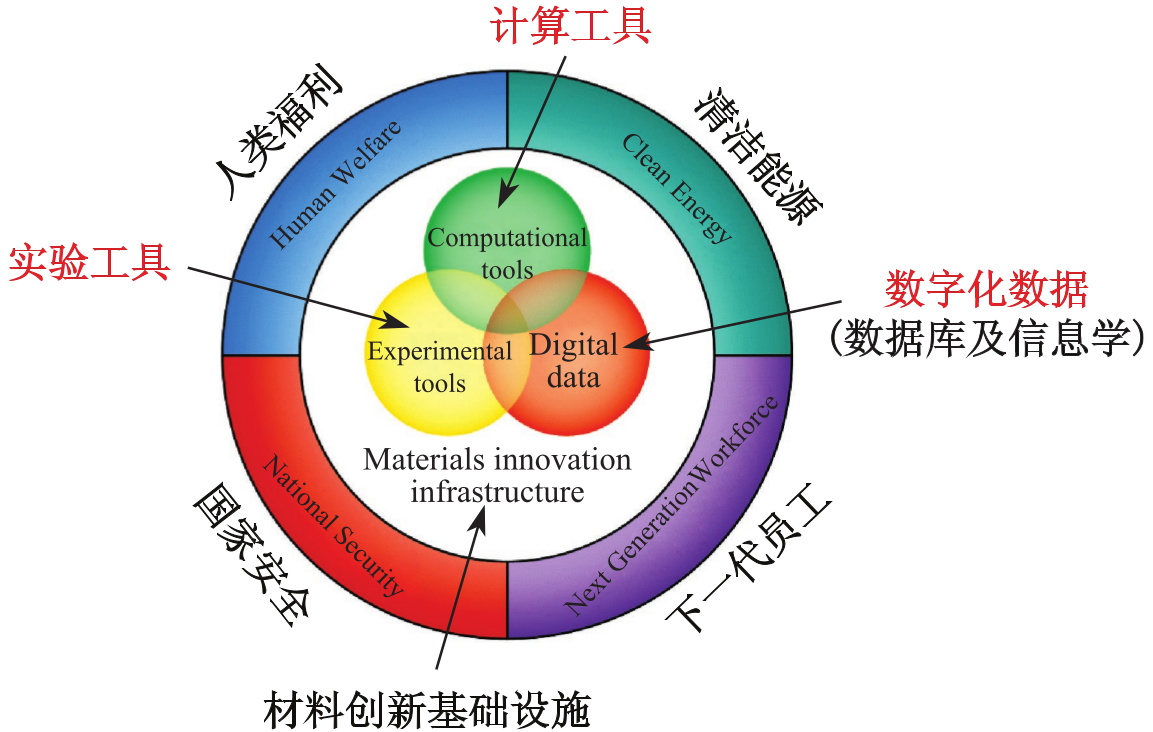
\includegraphics[height=2.55in,width=4.05in]{Figures/MGE.png}
%\caption{\tiny \textrm{Pseudopotential for metallic sodium, based on the empty core model and screened by the Thomas-Fermi dielectric function.}}%(与文献\cite{EPJB33-47_2003}图1对比)
%\caption{\tiny \textrm{Pseudopotential for metallic sodium, based on the empty core model and screened by the Thomas-Fermi dielectric function.}}%(与文献\cite{EPJB33-47_2003}图1对比)
\label{MGE}
\end{figure}
}

\frame
{
	\frametitle{材料模拟的基本思想和方法}
\begin{figure}[h!]
\vspace*{-0.25in}
\centering
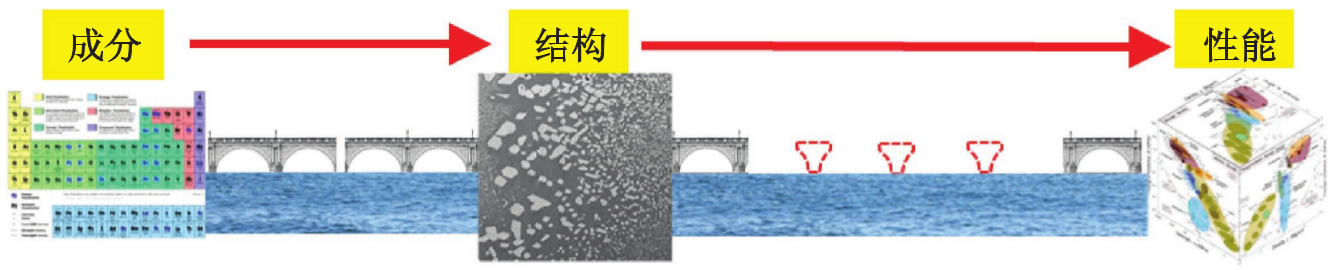
\includegraphics[height=0.80in,width=4.05in]{Figures/MGE-2.png}
%\caption{\tiny \textrm{Pseudopotential for metallic sodium, based on the empty core model and screened by the Thomas-Fermi dielectric function.}}%(与文献\cite{EPJB33-47_2003}图1对比)
\vskip 0.05pt
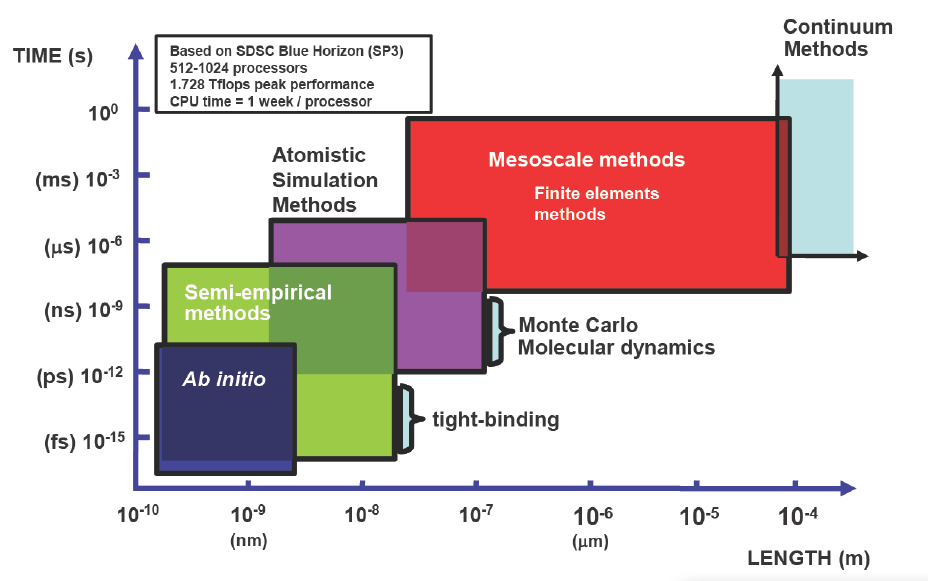
\includegraphics[height=2.20in,width=3.45in]{Figures/Multi-Scale-6.png}
%\caption{\tiny \textrm{Pseudopotential for metallic sodium, based on the empty core model and screened by the Thomas-Fermi dielectric function.}}%(与文献\cite{EPJB33-47_2003}图1对比)
\label{Multi-Scale}
\end{figure}
}

\frame
{
	\frametitle{\rm{I~Have~A~Dream}}
\begin{figure}[h!]
\vspace*{-0.18in}
\centering
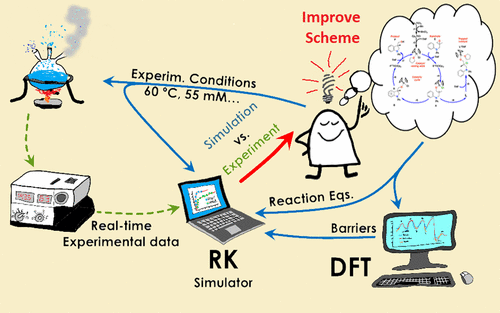
\includegraphics[height=2.55in,width=4.05in]{Figures/Schematic_Material-Design.png}
%\caption{\tiny \textrm{Pseudopotential for metallic sodium, based on the empty core model and screened by the Thomas-Fermi dielectric function.}}%(与文献\cite{EPJB33-47_2003}图1对比)
%\caption{\tiny \textrm{Pseudopotential for metallic sodium, based on the empty core model and screened by the Thomas-Fermi dielectric function.}}%(与文献\cite{EPJB33-47_2003}图1对比)
\label{Schematic_Material-Design}
\end{figure}
}

\section{量子力学基础}
\subsection{能量量子化}
\frame
{
	\frametitle{经典物理学天空的“两朵乌云”\textrm{(Dark Clouds)}}
\begin{figure}[h!]
\vspace*{-0.18in}
\centering
%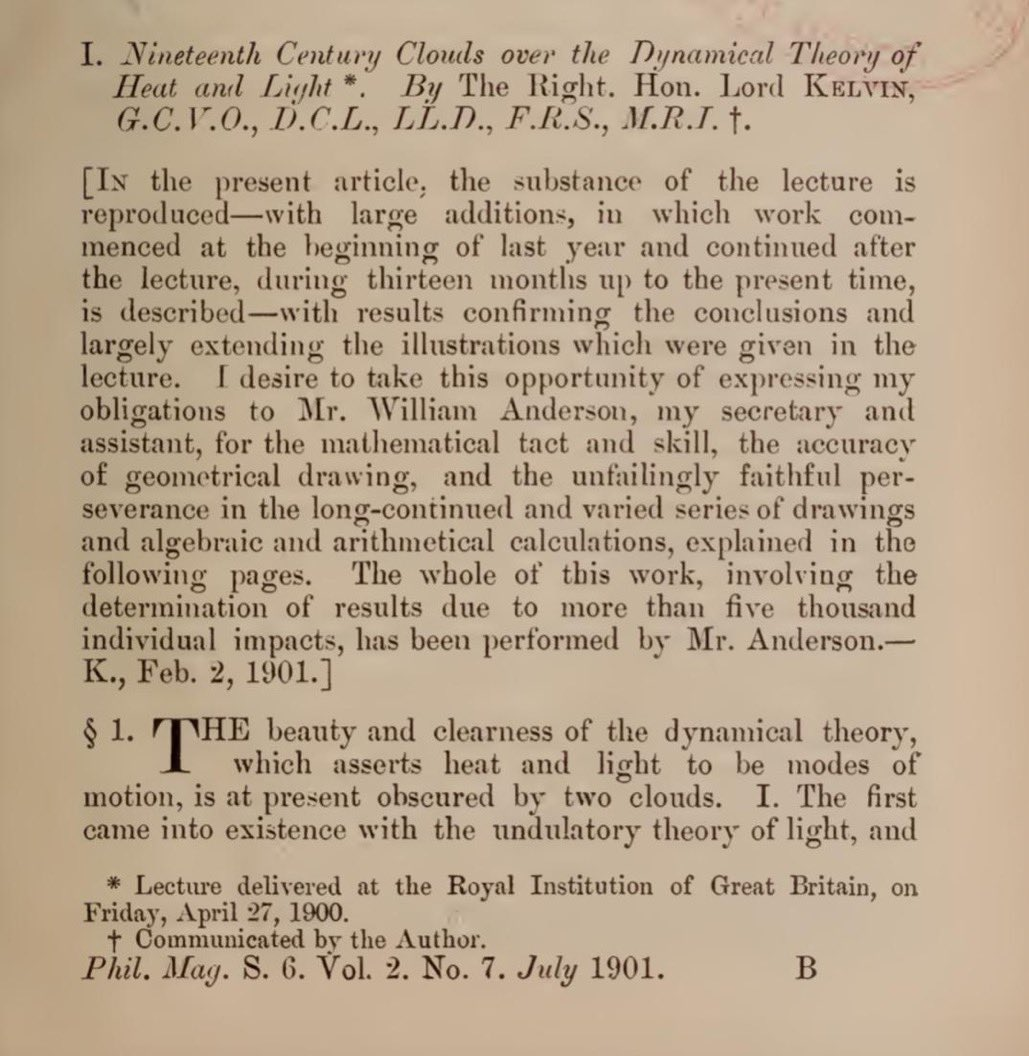
\includegraphics[height=2.90in,width=2.80in,viewport=0 0 1000 1100,clip]{Figures/Baron_Kelvin-Lecture.jpeg}
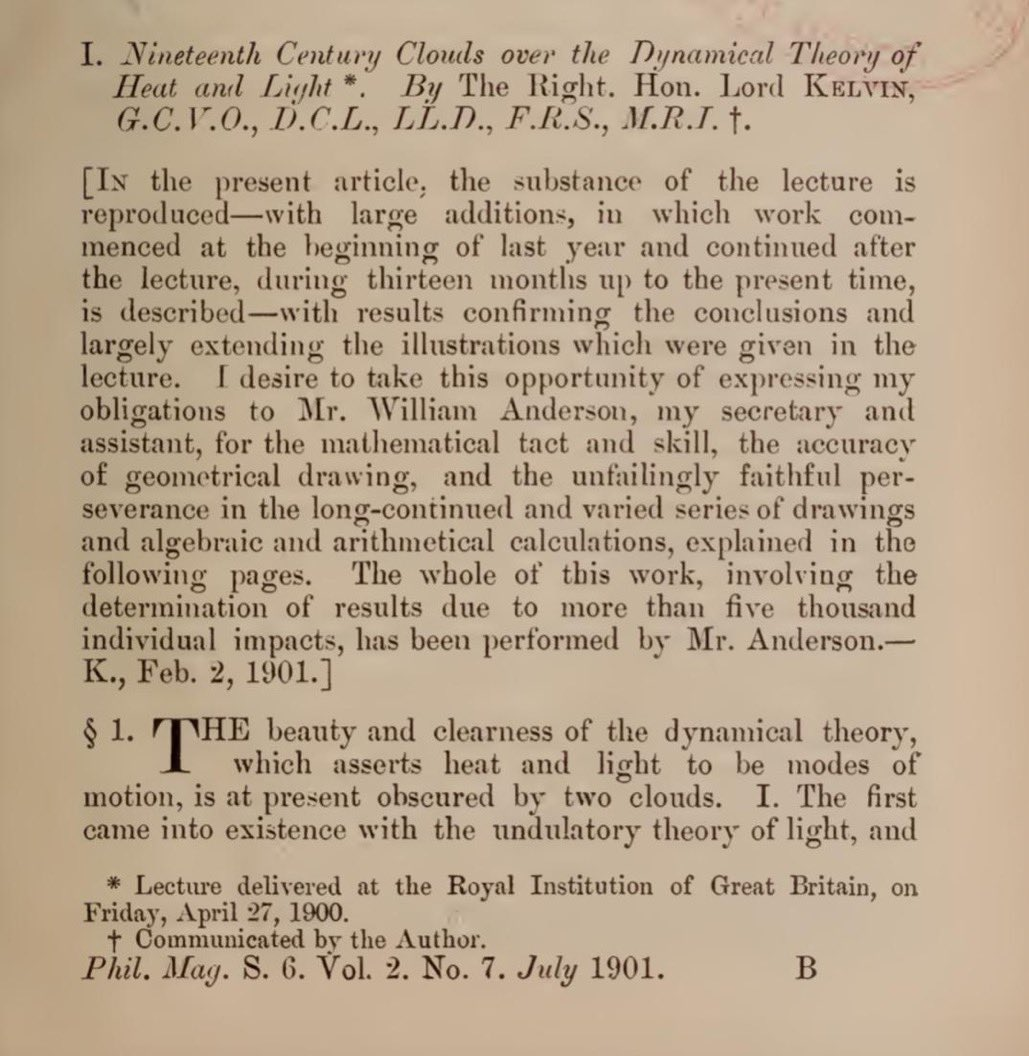
\includegraphics[height=0.35in,width=3.35in,viewport=0 900 1020 1030,clip]{Figures/Baron_Kelvin-Lecture.jpeg}
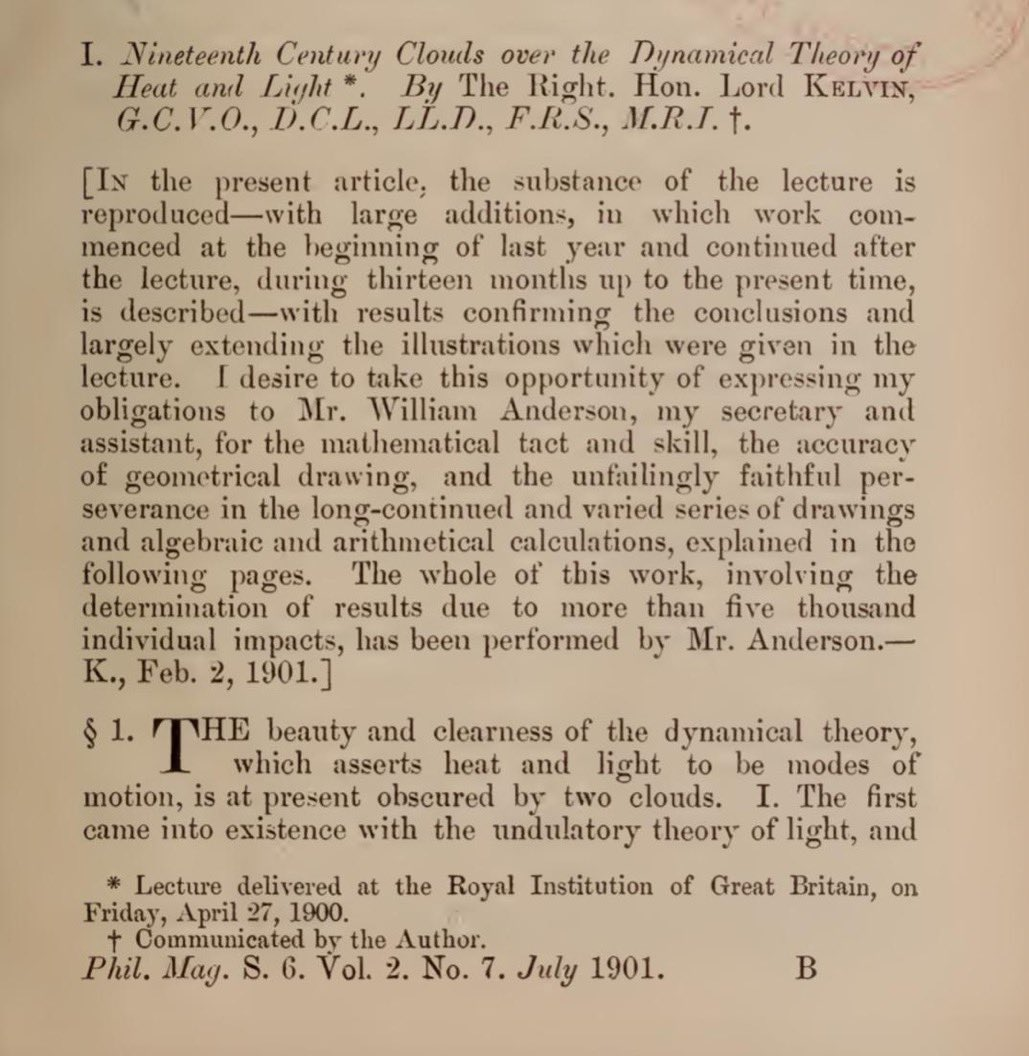
\includegraphics[height=0.80in,width=3.35in,viewport=0 50 1020 350,clip]{Figures/Baron_Kelvin-Lecture.jpeg}
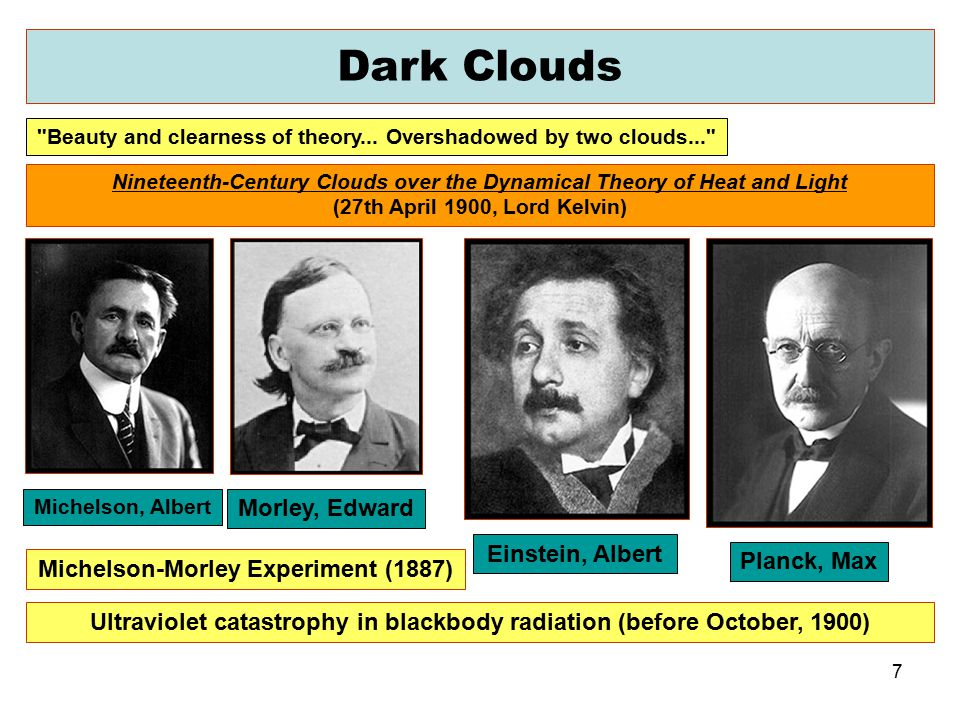
\includegraphics[height=1.85in,width=4.05in,viewport=0 50 735 370,clip]{Figures/Two-dark-cloud-in-physics-2.jpg}
\label{two_Dark_Clouds_2}
\end{figure}
}

%\frame
%{
%	\frametitle{经典物理学天空的“两朵乌云”\textrm{(Dark Clouds)}}
%\begin{figure}[h!]
%\vspace*{-0.18in}
%\centering
%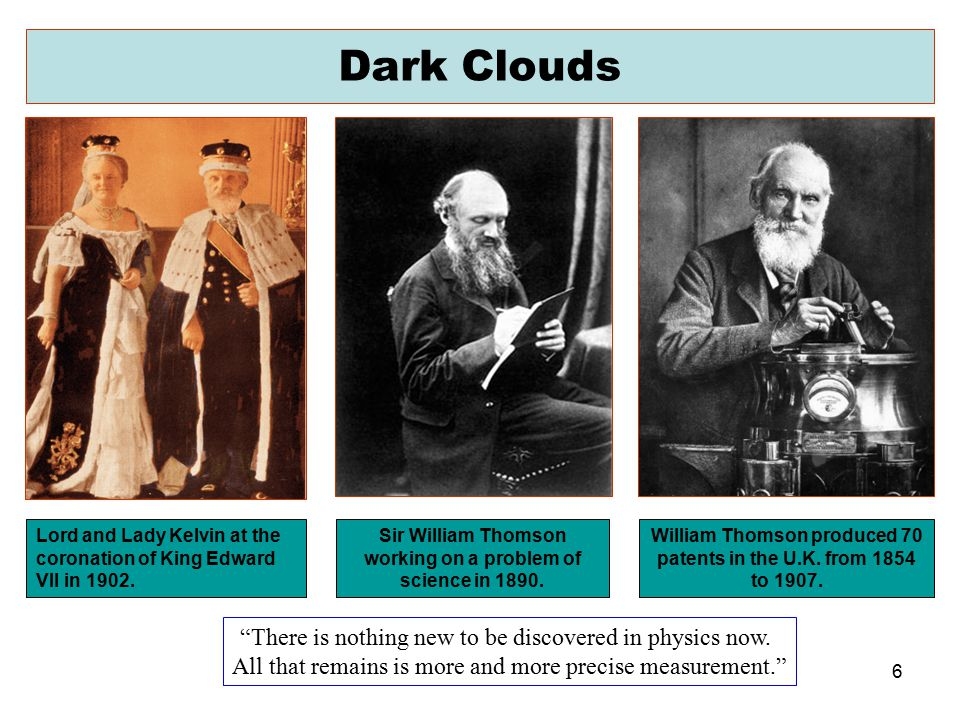
\includegraphics[height=2.50in,width=4.05in,viewport=0 20 735 470,clip]{Figures/Two-dark-cloud-in-physics-3.jpg}
%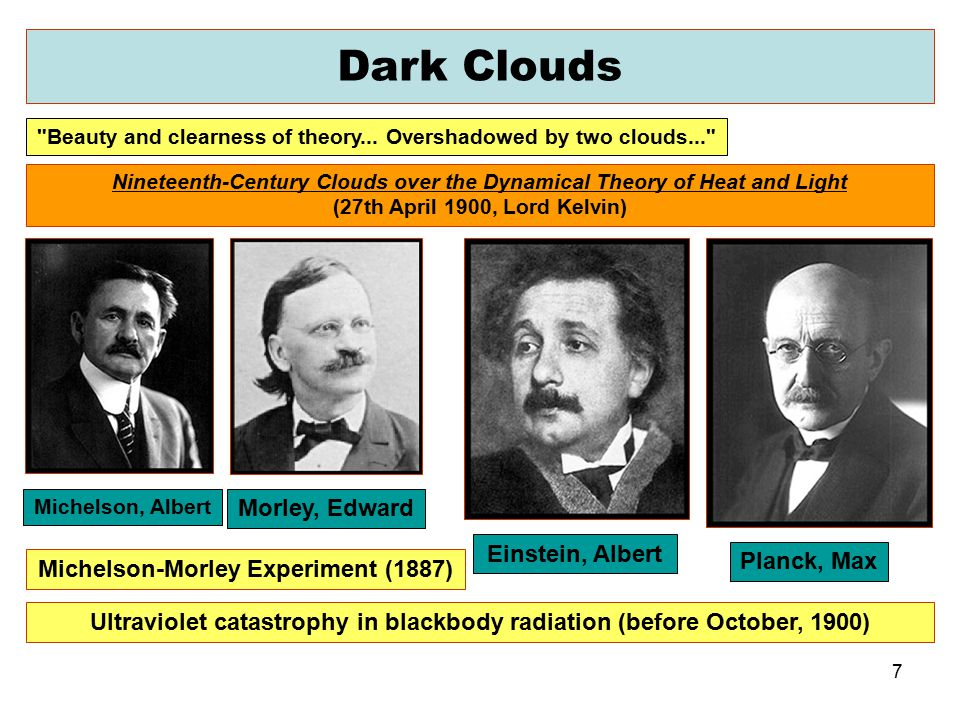
\includegraphics[height=2.40in,width=4.05in,viewport=0 50 735 470,clip]{Figures/Two-dark-cloud-in-physics-2.jpg}
%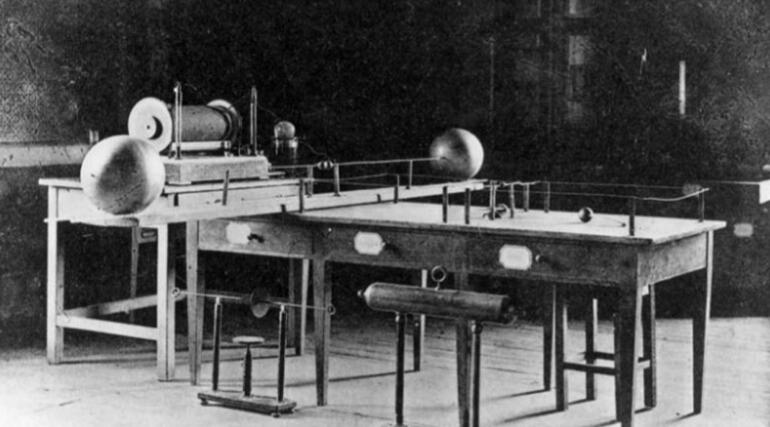
\includegraphics[height=2.40in,width=4.05in,viewport=0 0 580 325,clip]{Figures/Two-dark-cloud-in-physics-1.jpg}
%\label{two_Dark_Clouds_3}
%\end{figure}
%}
%
\frame
{
	\frametitle{黑体辐射与能量量子化}
	\textrm{1900}年,为了解释黑体辐射\textrm{(black-body radiation)}的能量密度与电磁辐射频率的关系,\textrm{M.~Planck}%放弃\textcolor{blue}{能量均分定理}\textrm{(the equipartition theorem)},
	引入\textcolor{red}{能量量子化}\textrm{(quantization of energy)}的假设,利用统计物理推导出与实验符合得非常好的黑体辐射\textrm{Planck~}公式:~
	\begin{displaymath}
		\rho_{\nu}\mathrm{d}{\nu}=\dfrac{8{\pi}h{\nu}^3}{C^2}\bigg(\dfrac1{\mathrm{e}^{h\nu/kT}-1}\bigg)\mathrm{d}\nu
	\end{displaymath}
\begin{figure}[h!]
\centering
\vspace{-10.5pt}
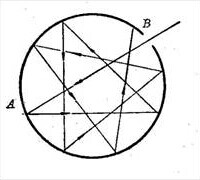
\includegraphics[height=1.45in,width=1.45in,viewport=0 0 136 136,clip]{Figures/Black_box.jpg}
\hskip 1pt
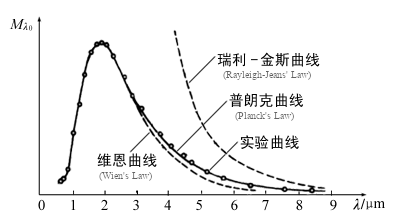
\includegraphics[height=1.32in,width=2.25in,viewport=0 0 390 215,clip]{Figures/Black_box_curve.png}
\caption{\textrm{The black-body radiation and the curve}}
\label{Black_box}
\end{figure}
}

\frame
{
	\frametitle{波-粒二象性与光电效应}
\begin{figure}[h!]
\centering
\vspace{-15.5pt}
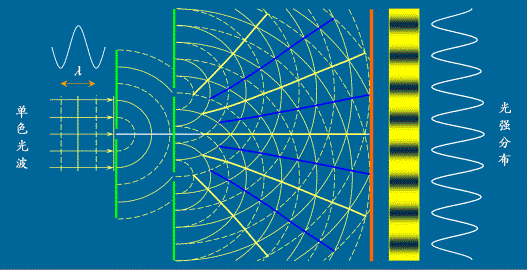
\includegraphics[height=1.35in,width=2.70in,viewport=0 0 536 280,clip]{Figures/wave-particle_duality.png}
\vskip 1pt
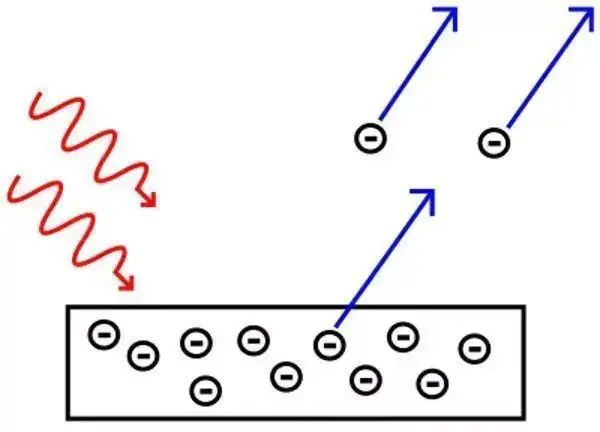
\includegraphics[height=1.32in,width=2.05in,viewport=0 0 620 455,clip]{Figures/Photoelectic_effect.png}
\caption{\textrm{The wave-particle duality and Photoelectric effect}}
\label{wave_and_particle}
\end{figure}
}

\frame
{
	\frametitle{电子衍射、\textrm{Compton~effect}与\textrm{H}原子光谱}
\begin{figure}[h!]
\centering
\vspace{-15.5pt}
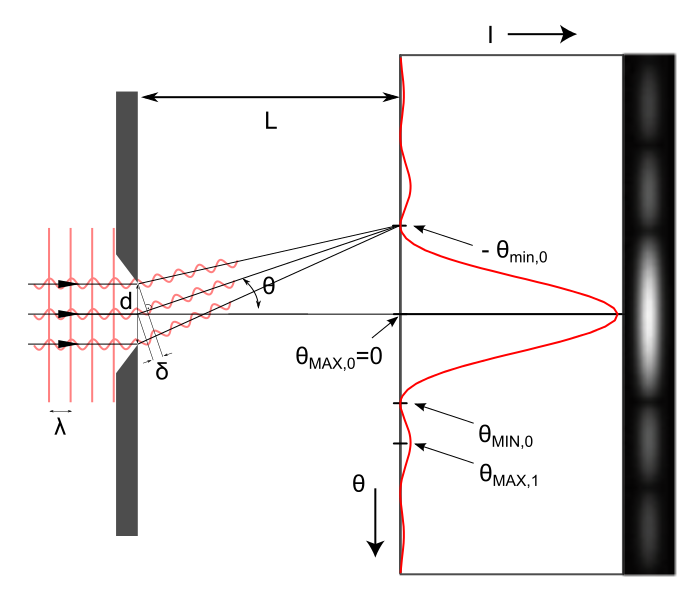
\includegraphics[height=1.35in,width=1.80in,viewport=0 0 680 600,clip]{Figures/Single_Slit_Diffraction.png}
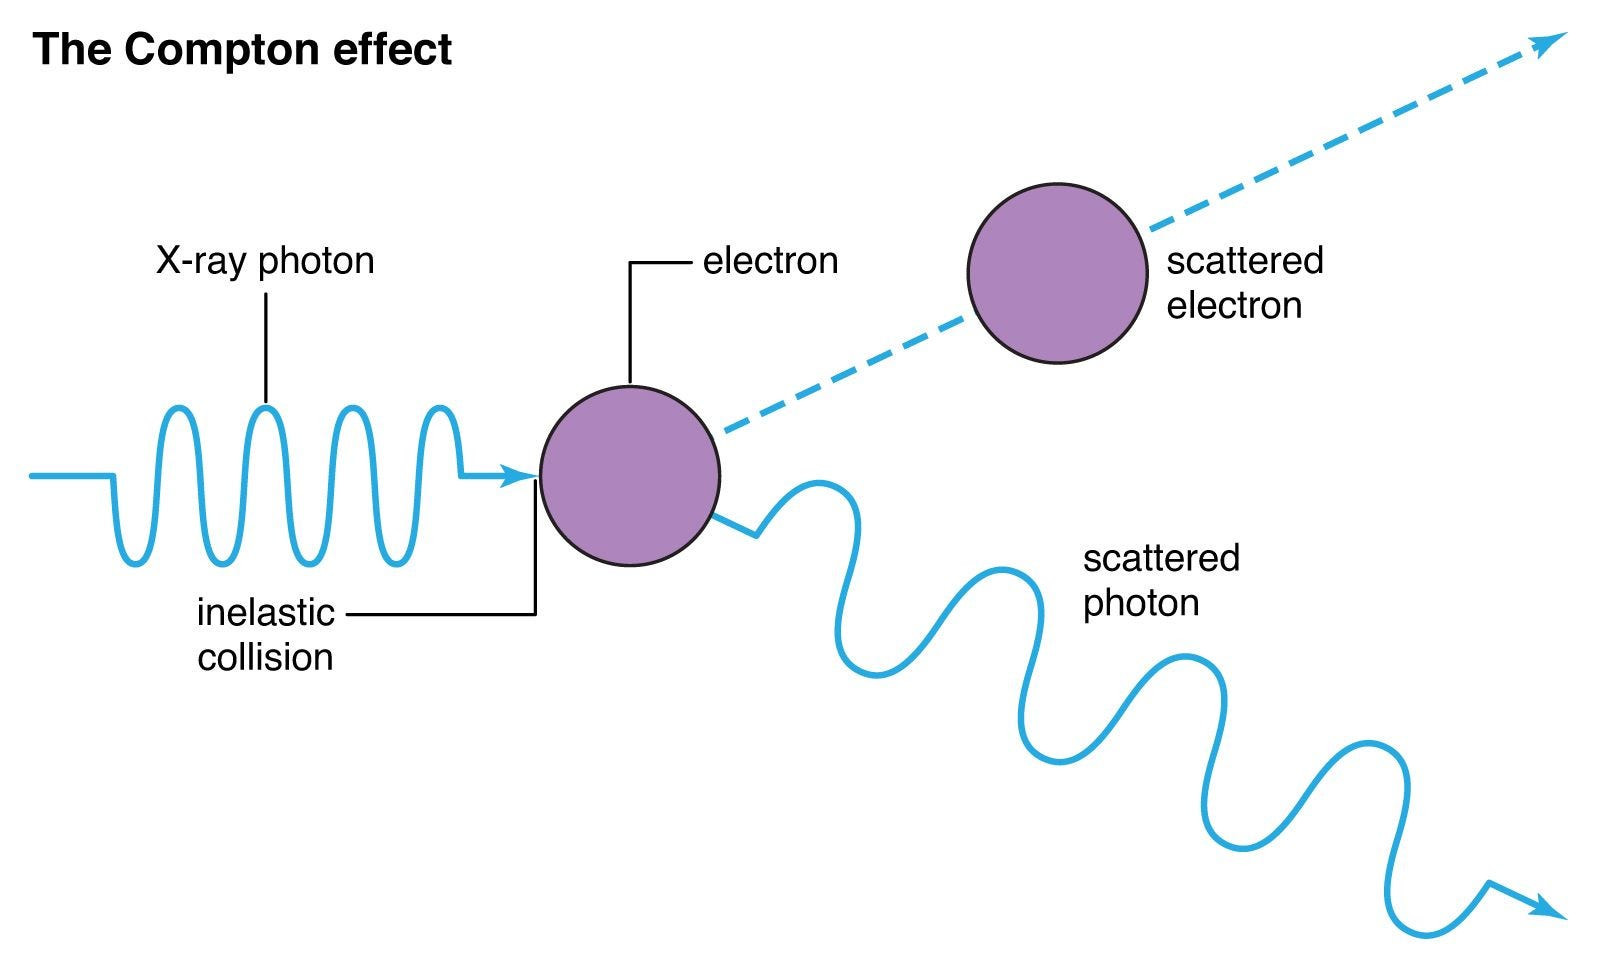
\includegraphics[height=1.20in,width=2.10in,viewport=0 0 1600 950,clip]{Figures/Compton_effect.jpg}\\
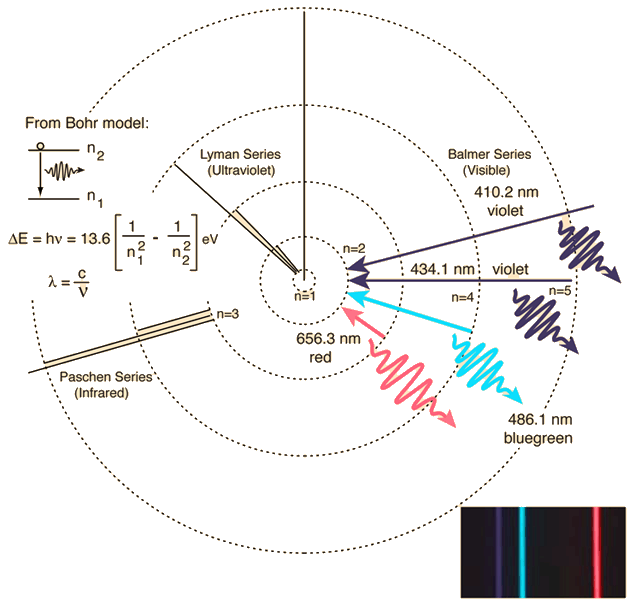
\includegraphics[height=1.65in,width=1.75in,viewport=0 0 620 600,clip]{Figures/Hydrogen_spectrum-3.png}
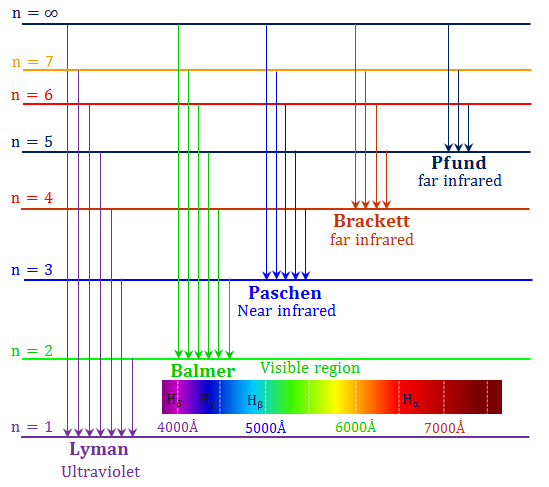
\includegraphics[height=1.55in,width=1.75in,viewport=0 0 500 380,clip]{Figures/Hydrogen_spectrum-2.png}
%\caption{\textrm{The wave-particle duality and Photoelectric effect}}
\label{electron:wave_and_particle}
\end{figure}
}

\subsection{\textrm{Schr\"odinger}方程与量子力学的建立}
\frame
{
	\frametitle{\textrm{De Broglie}物质波}
\begin{minipage}{0.53\textwidth}
\begin{figure}[h!]
\centering
\vspace{-15.5pt}
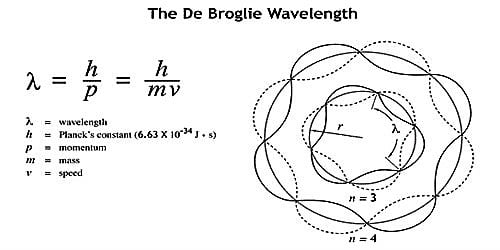
\includegraphics[height=1.3in,width=2.1in,viewport=0 0 500 280,clip]{Figures/De-Broglie-waves.jpg}
%\caption{\textrm{The wave-particle duality and Photoelectric effect}}
\label{Matter_wave}
\end{figure}
经典的观念:
\begin{itemize}
	\item \textcolor{red}{粒子}:~\textcolor{blue}{物质存在的形式}
	\item \textcolor{red}{波动}:~\textcolor{blue}{能量传递的形式}
\end{itemize}
\end{minipage}
\begin{minipage}{0.45\textwidth}
\begin{figure}[h!]
\centering
\vspace{-15.5pt}
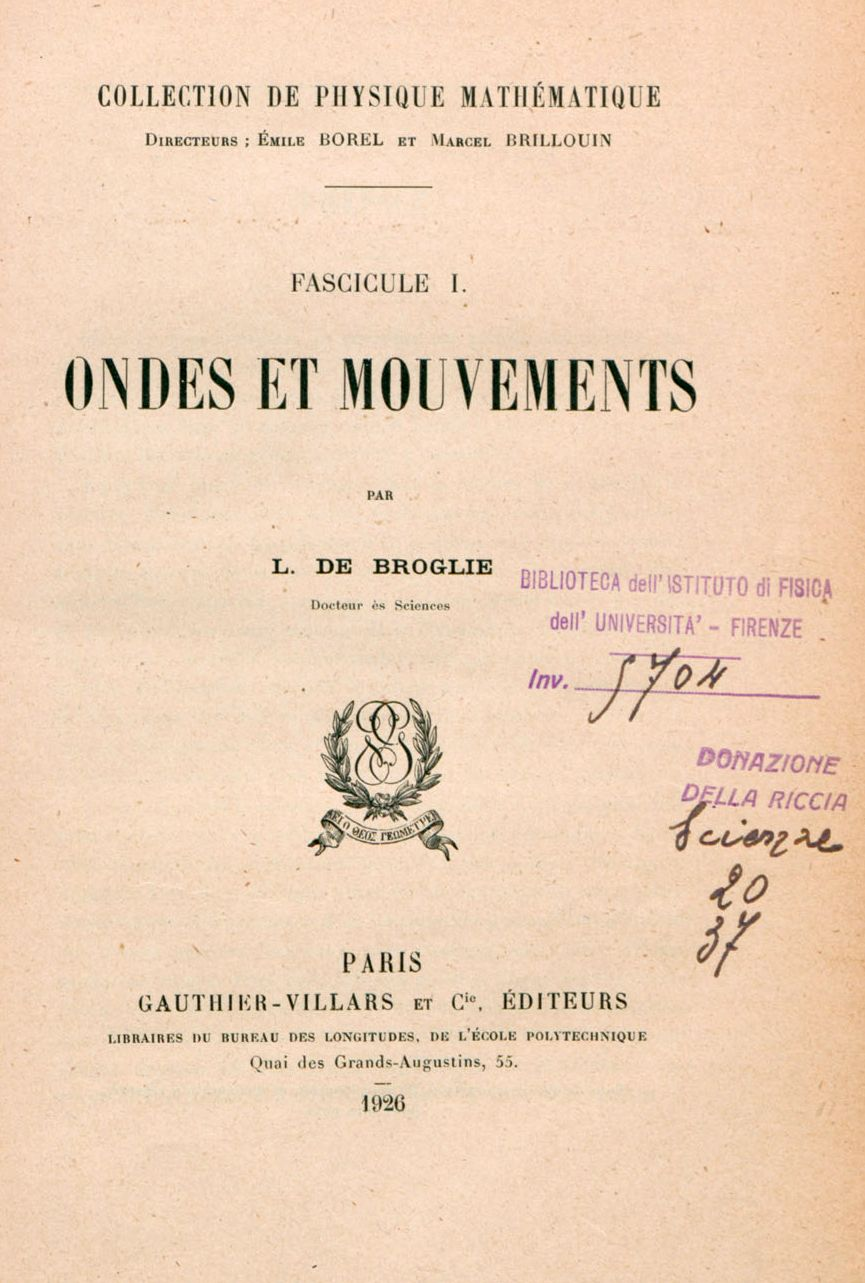
\includegraphics[height=2.80in,width=1.90in,viewport=0 0 430 650,clip]{Figures/De_Broglie-dissertation_Cover.jpg}
%\caption{\textrm{The wave-particle duality and Photoelectric effect}}
\label{De_Broglie-dissertation}
\end{figure}
\end{minipage}
}

\frame
{
	\frametitle{驻波}
\begin{figure}[h!]
\centering
\vspace{-15.5pt}
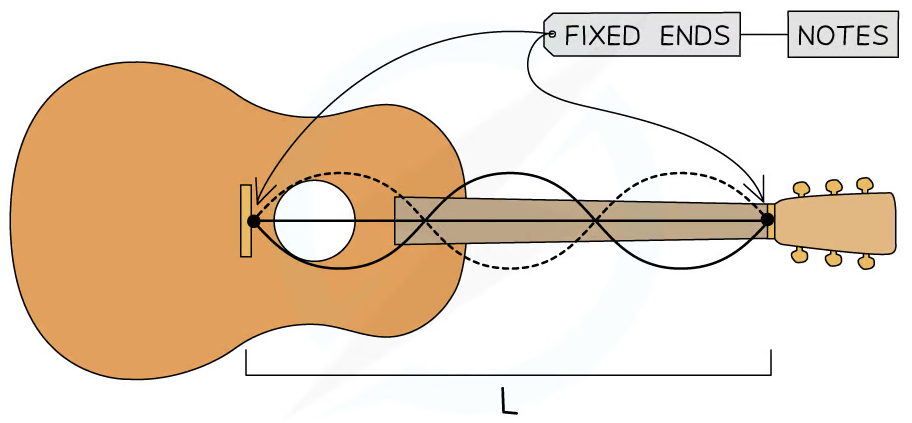
\includegraphics[height=0.40\textwidth,width=0.8\textwidth,viewport=0 0 900 450,clip]{Figures/Guitar-string.png}
\vskip 0.1pt
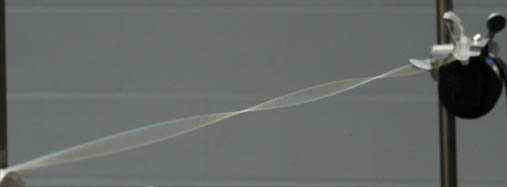
\includegraphics[height=0.35\textwidth,width=0.8\textwidth,viewport=0 0 122 48,clip]{Figures/string-standing-wave.jpg}
%\caption{\textrm{ABINIT}的Si.in}
\label{Standing_Wave_0}
\end{figure}
}

\frame
{
	\frametitle{驻波方程与势阱}
\begin{figure}[h!]
\centering
\vspace{-12.5pt}
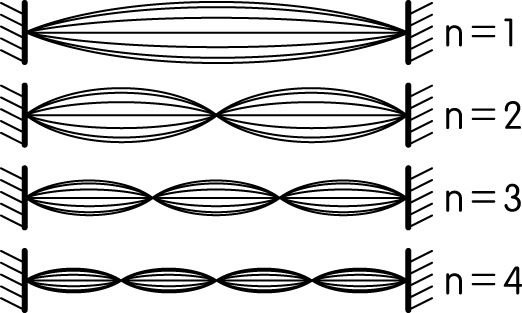
\includegraphics[height=0.32\textwidth,width=0.7\textwidth,viewport=0 0 125 75,clip]{Figures/Standing_wave.jpeg}
\vskip 2pt
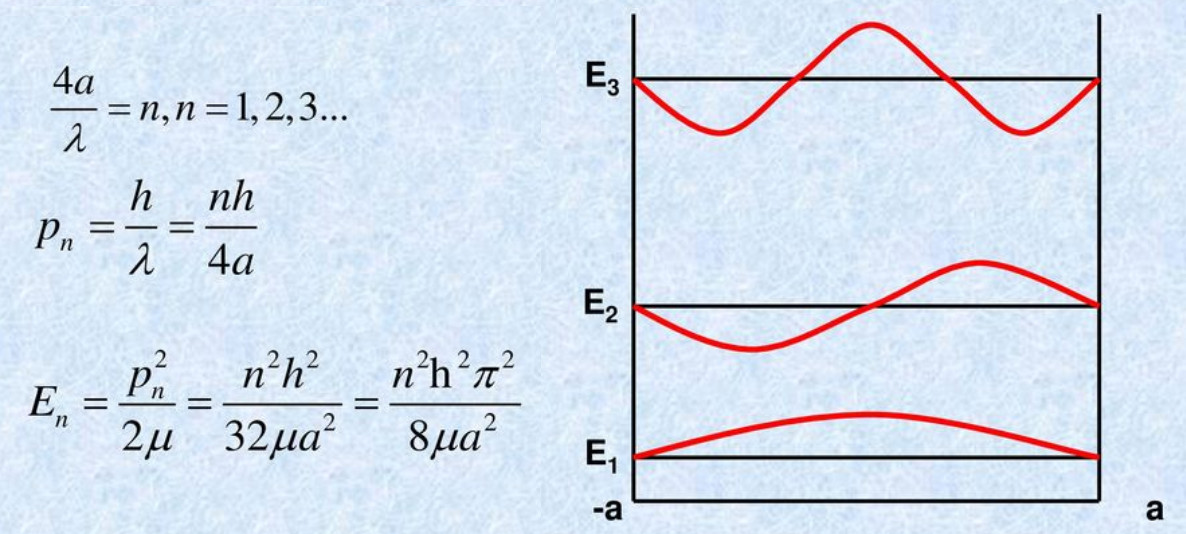
\includegraphics[height=0.40\textwidth,width=0.9\textwidth,viewport=0 0 1200 550,clip]{Figures/Standing_wave-energy.jpg}
%\caption{\textrm{ABINIT}的Si.in}
\label{Standing_Wave_1}
\end{figure}
}

\frame
{
	\frametitle{原子中电子的驻波方程}
\begin{figure}[h!]
	\vspace{-10.5pt}
\centering
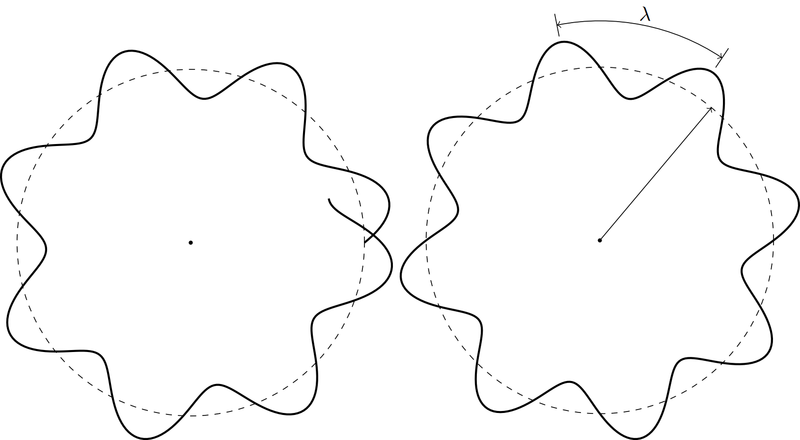
\includegraphics[height=0.38\textwidth,width=0.74\textwidth,viewport=0 0 840 440,clip]{Figures/Standing_wave-atom.png}
\vskip 2pt
\animategraphics[autoplay, loop, height=1.3in]{1}{Figures/Standing_wave_circle_}{1}{25}
\label{Atomic-electron_Standing_wave}
\end{figure}
}

\frame
{
	\frametitle{原子中的电子轨道和能量}
\begin{minipage}{0.43\textwidth}
\begin{figure}[h!]
%	\vspace{-14.8pt}
	\vspace{-4.8pt}
\centering
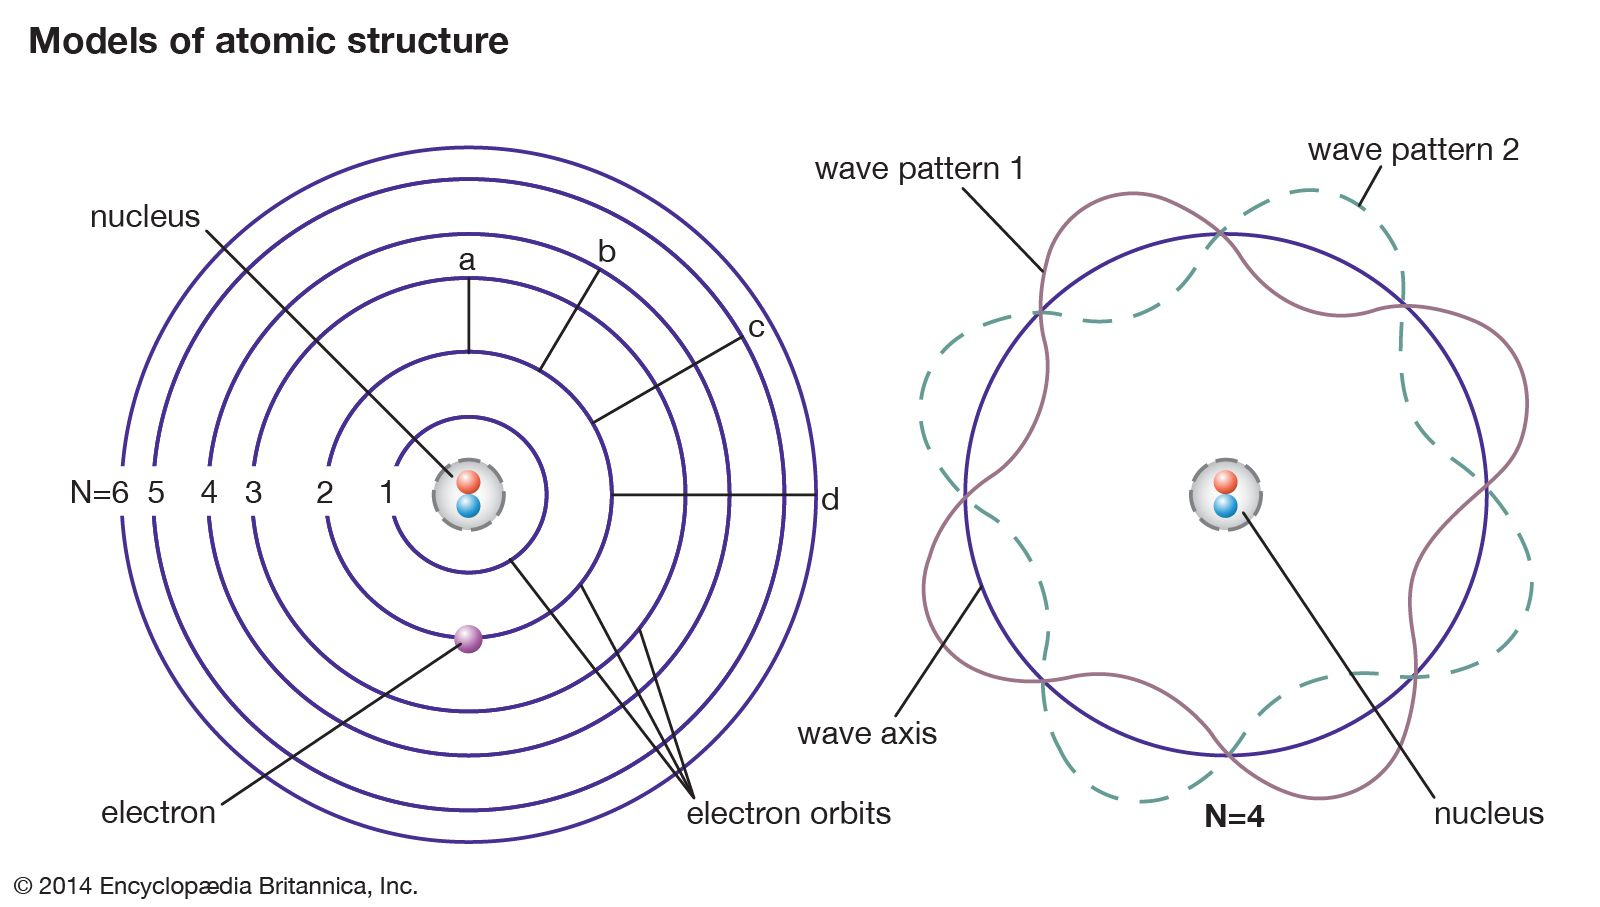
\includegraphics[height=0.57\textwidth,width=1.00\textwidth,viewport=0 50 1680 1000,clip]{Figures/electron-theory-Bohr-point-mass-energy-levels.jpg}
%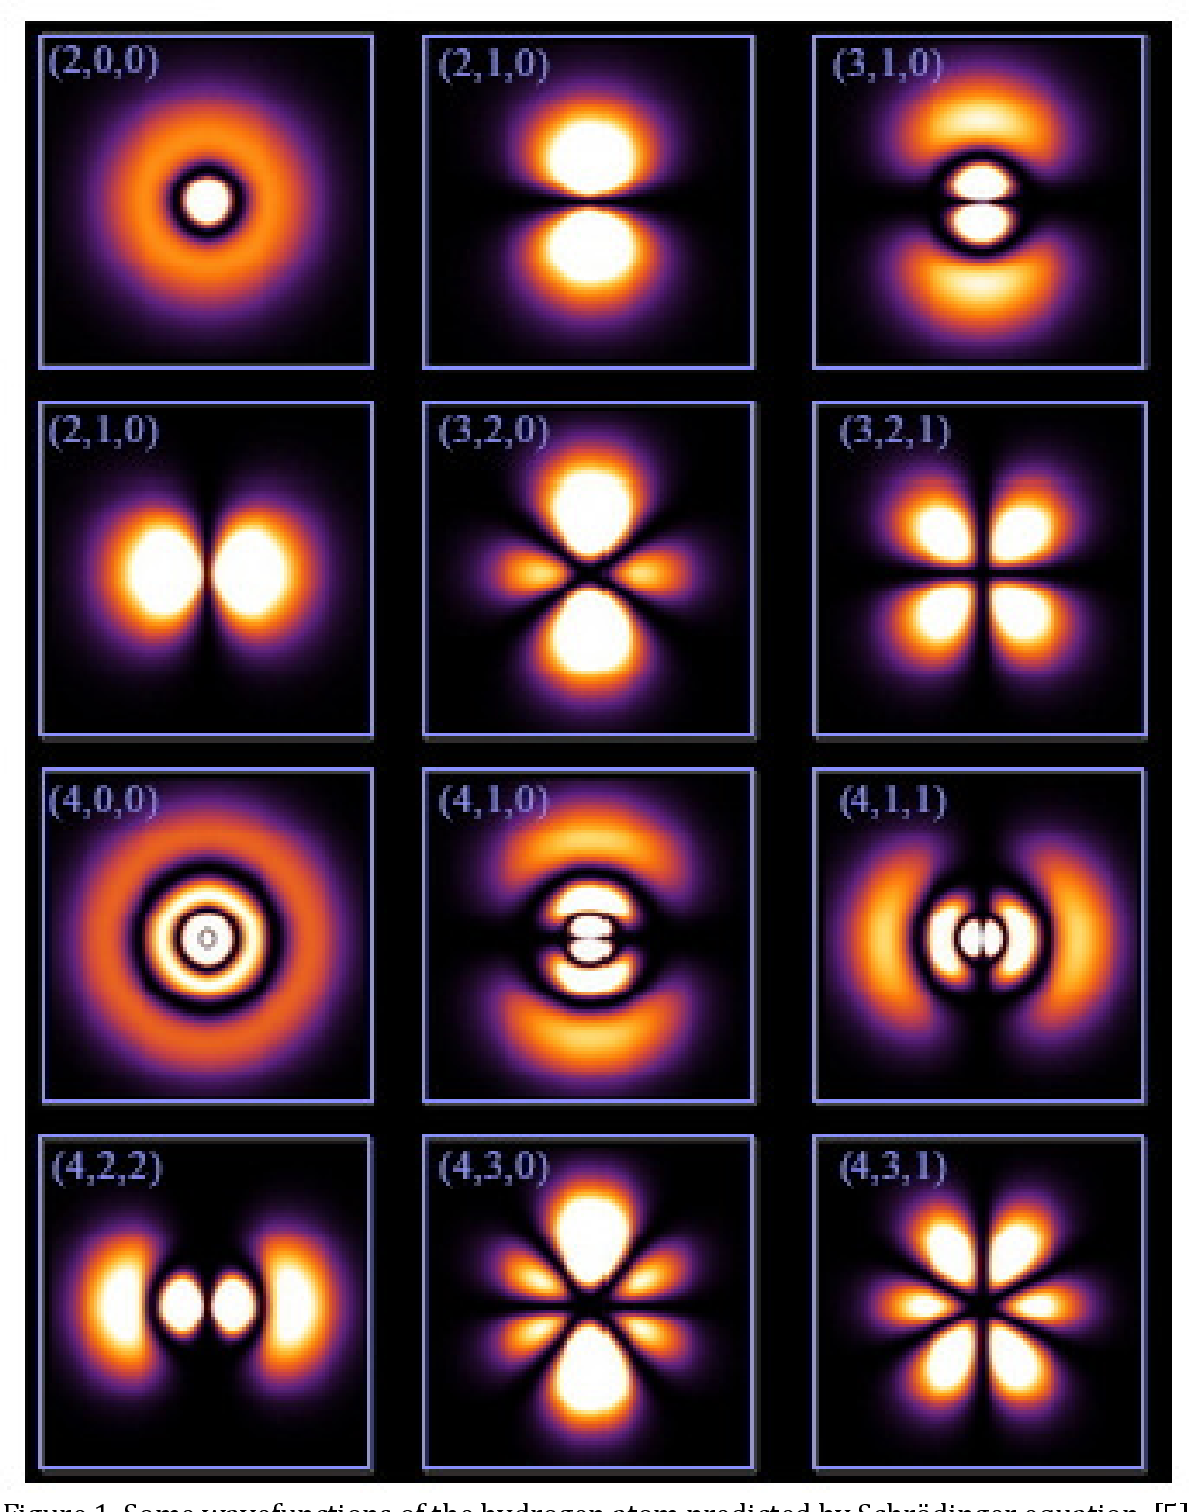
\includegraphics[height=1.23\textwidth,width=1.00\textwidth,viewport=0 10 1250 1500,clip]{Figures/wave_function.png}
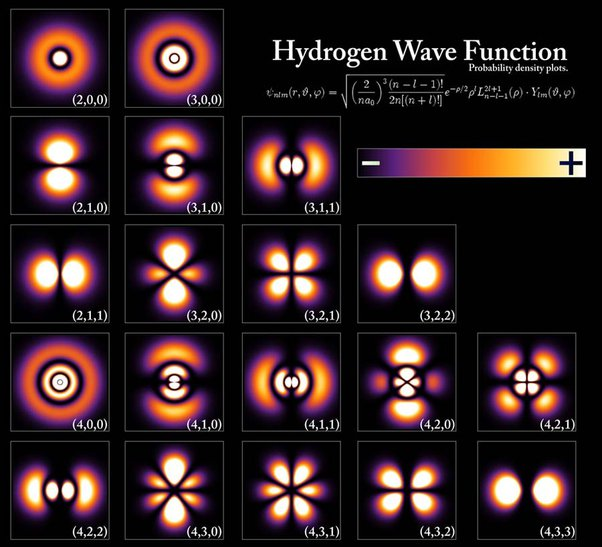
\includegraphics[height=0.95\textwidth,width=1.00\textwidth,viewport=0 0 630 650,clip]{Figures/wave_function-2.jpeg}
\label{Atomic-electron_wave}
\end{figure}
\end{minipage}
\begin{minipage}{0.55\textwidth}
\begin{figure}[h!]
	\vspace{-16.5pt}
\centering
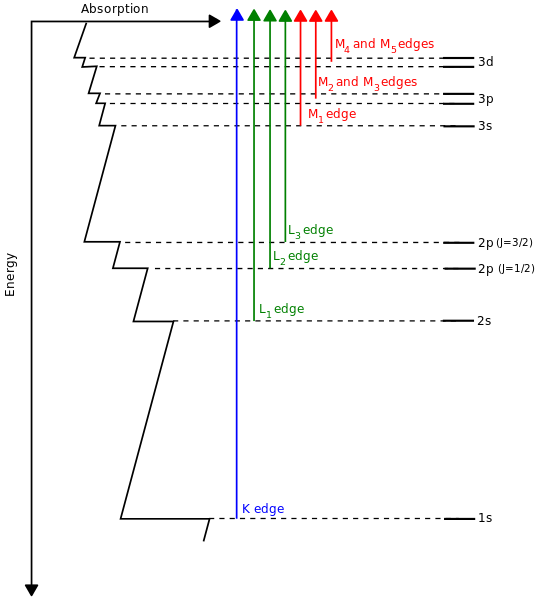
\includegraphics[height=1.10\textwidth,width=1.00\textwidth,viewport=0 0 560 600,clip]{Figures/Electron_orbital-energy.png}
\label{Atomic-electron_wave-energy}
\end{figure}
\end{minipage}
}

\frame
{
	\frametitle{\textrm{Schr\"odinger}~方程}
\begin{minipage}{0.49\textwidth}
\begin{figure}[h!]
\centering
%
\vspace{-25.5pt}
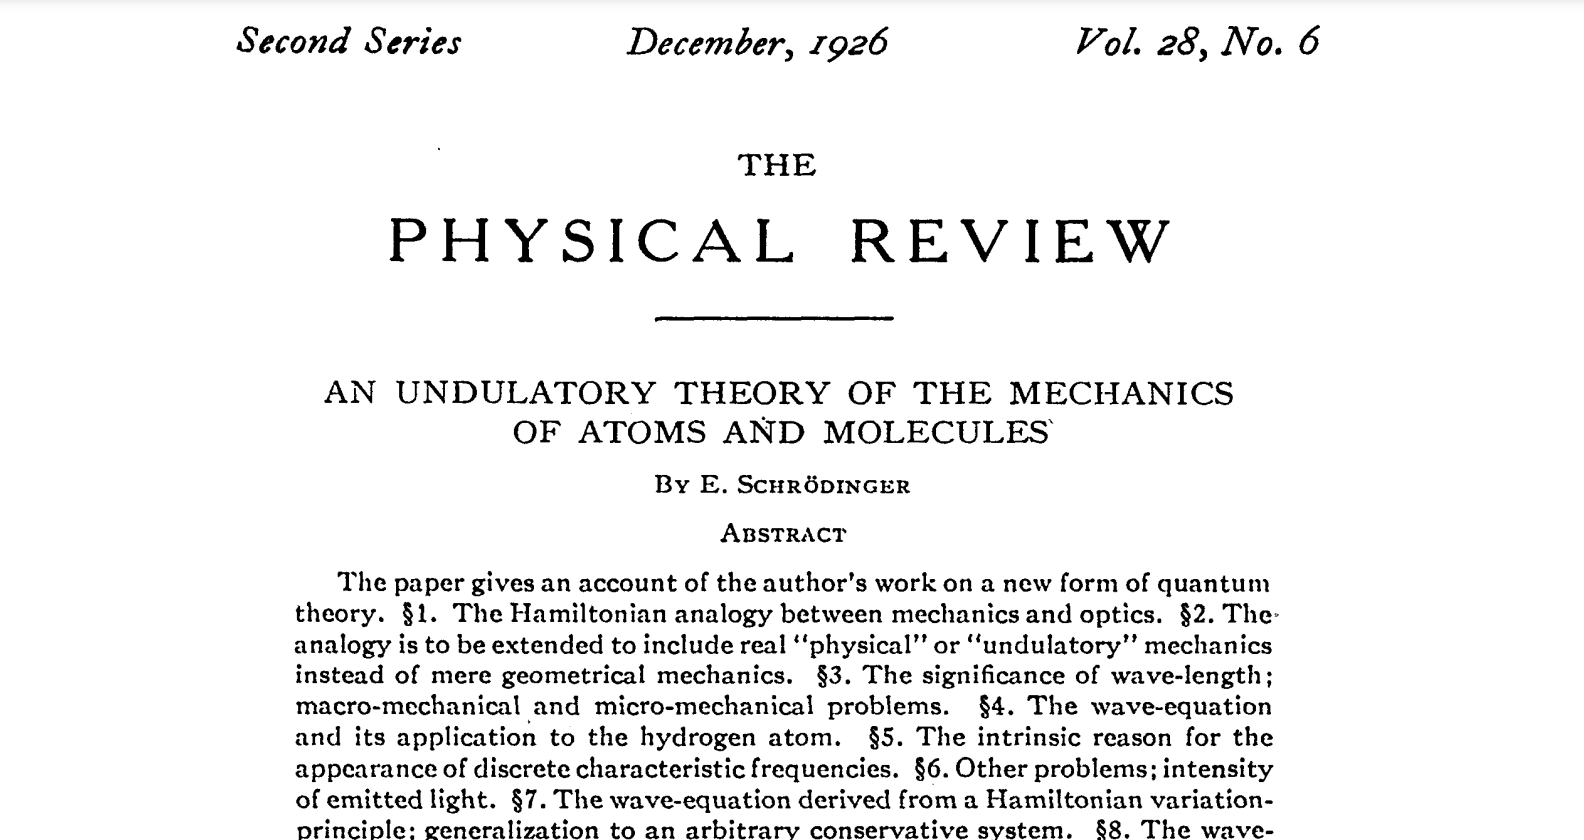
\includegraphics[height=1.80in,width=2.00in,viewport=180 0 1380 1100,clip]{Figures/Schrodinger_article.png}
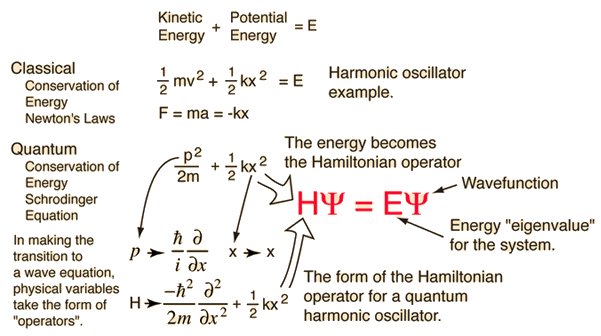
\includegraphics[height=1.20in,width=2.00in,viewport=0 0 600 350,clip]{Figures/Schrodinger_Equation.png}
\label{Schrodinger_Equation}
\end{figure}
\end{minipage}
\begin{minipage}{0.49\textwidth}
\begin{figure}[h!]
\centering
%
\vspace{-15.5pt}
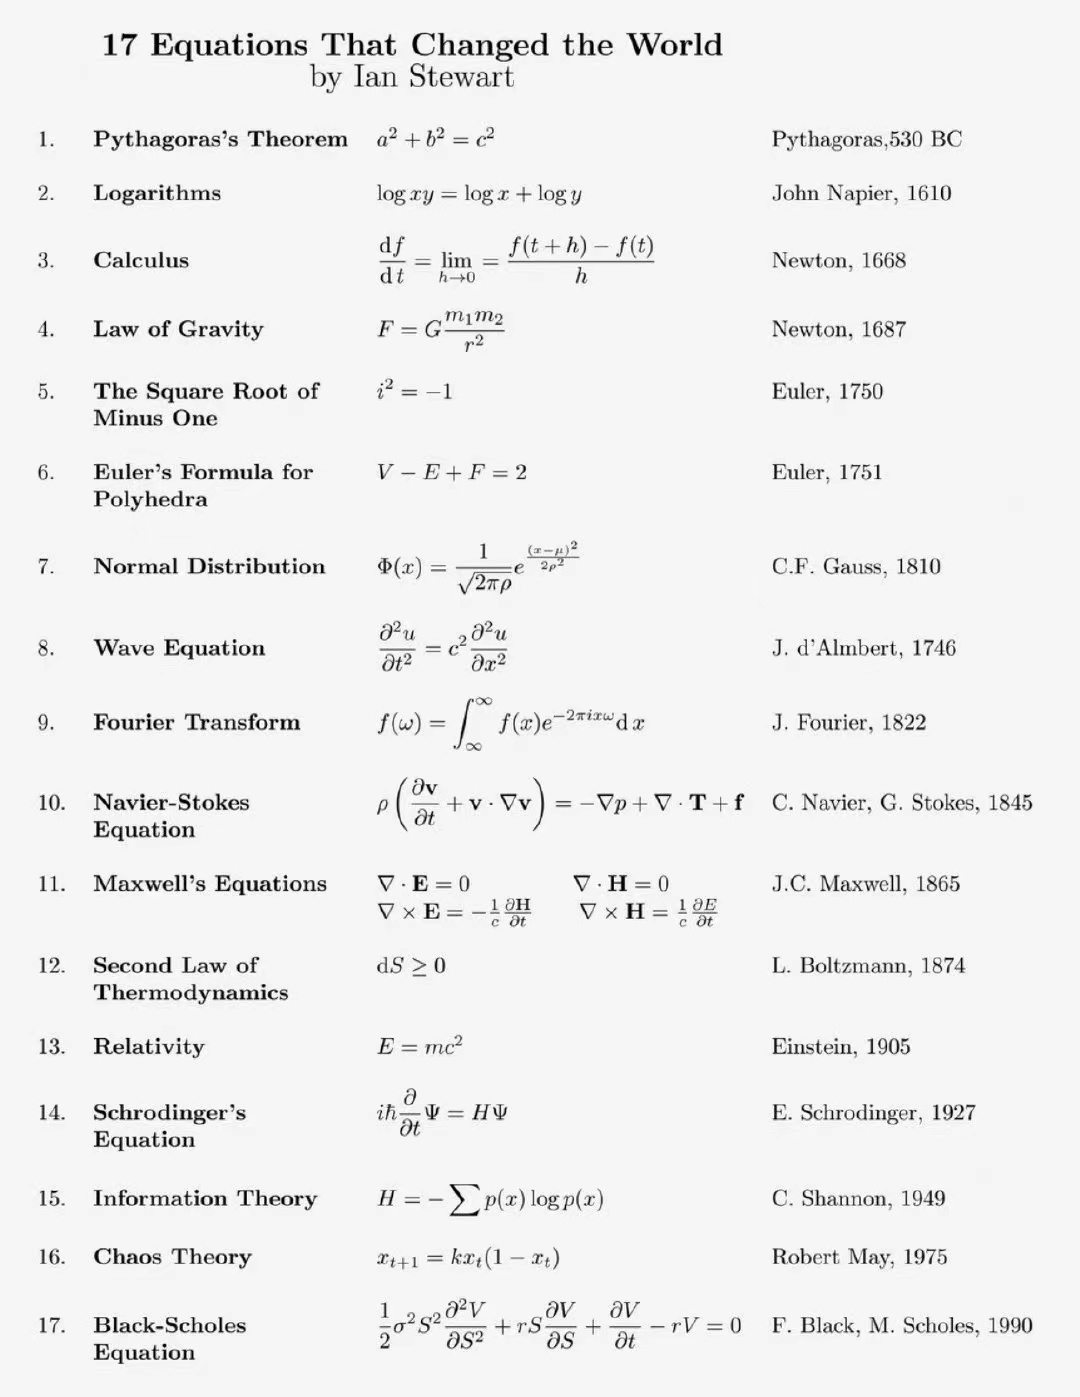
\includegraphics[height=2.85in,width=2.00in,viewport=0 0 780 1100,clip]{Figures/Great_Equation.jpg}
\label{Great_Equation}
\end{figure}
\end{minipage}
}

\frame
{
	\frametitle{量子力学的奠基人}
\begin{figure}[h!]
\centering
%\vspace{-25.5pt}
%\hspace*{-15.5pt}
%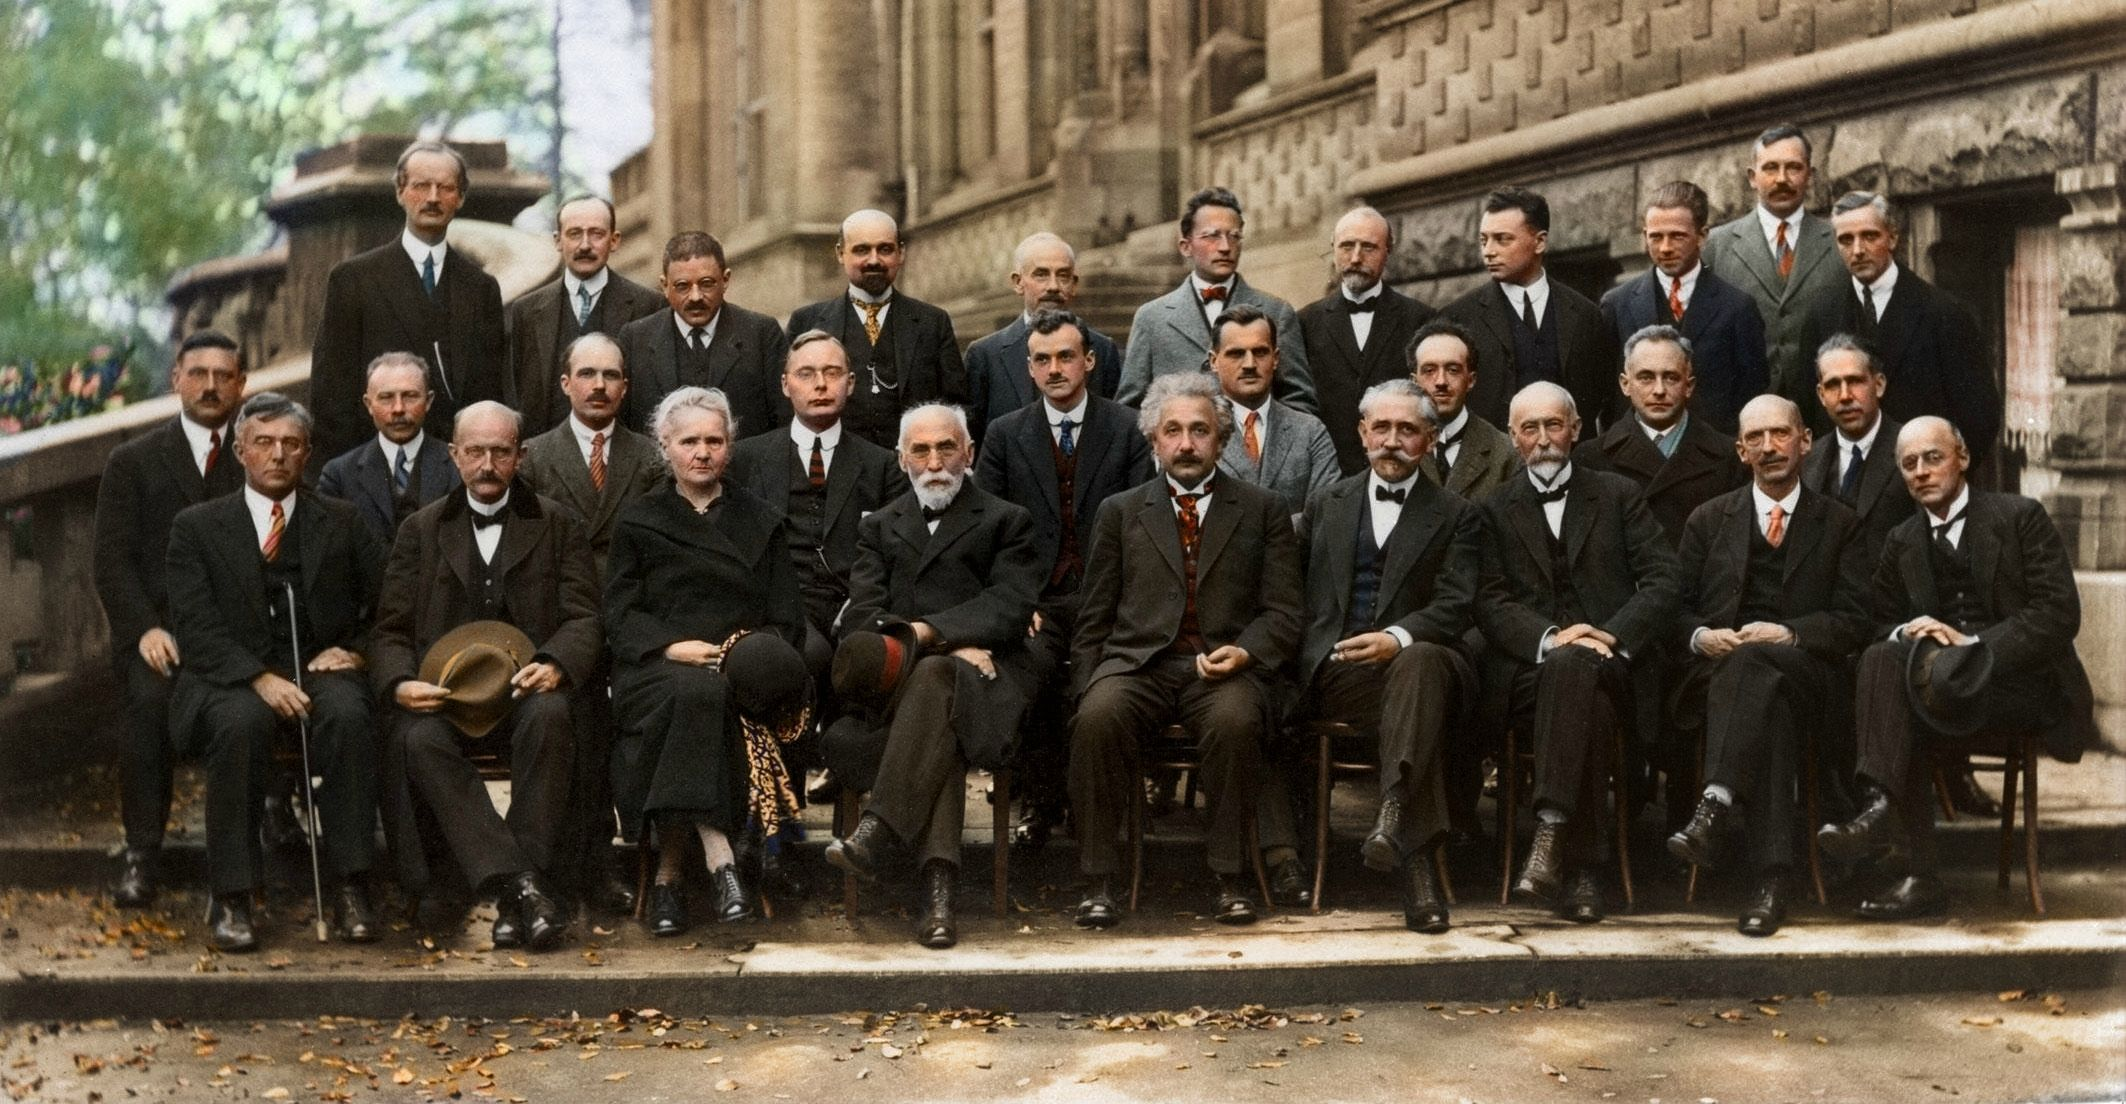
\includegraphics[height=0.57\textwidth,width=1.1\textwidth,viewport=0 0 2150 1050,clip]{Figures/Solvay_Conference-5-fine.jpg}
\vspace{-14.5pt}
\hspace*{-15.5pt}
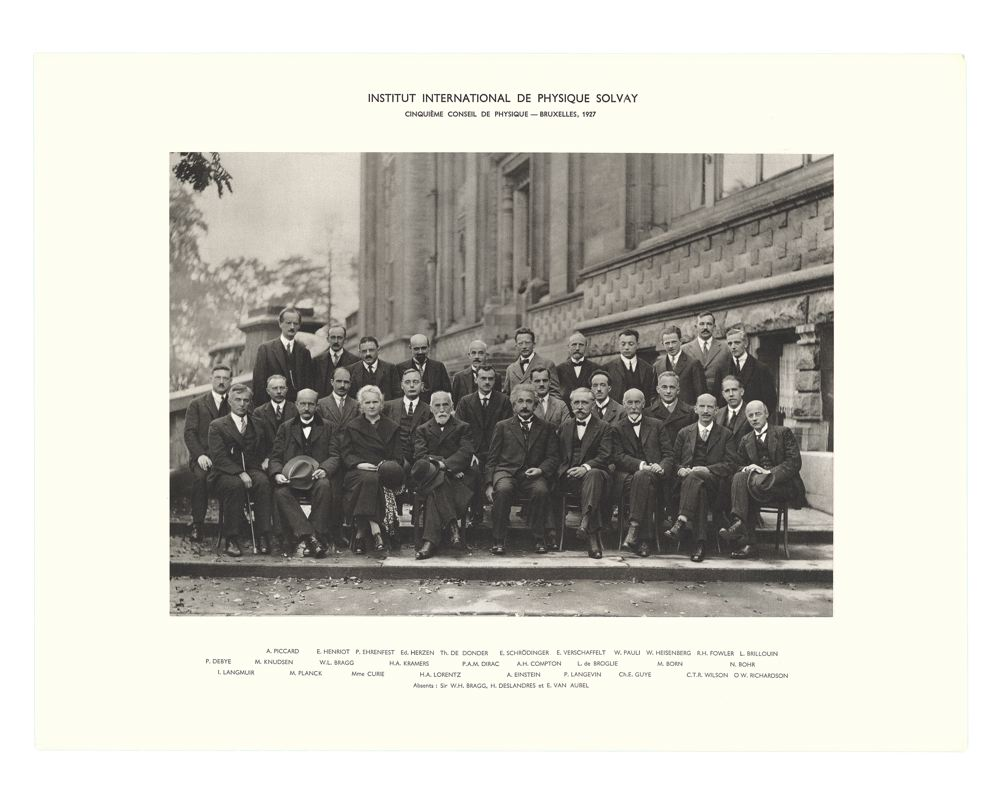
\includegraphics[height=0.50\textwidth,width=0.70\textwidth,viewport=150 105 850 710,clip]{Figures/Solvay_Conference-5.jpg}
\caption{\fontsize{7.5pt}{6.2pt}\selectfont{\textrm{The Fifth Solvay International Conference, Brussels, Belgium, Oct. 1927}}}
\label{Solvay Conference-5-fine}
\end{figure}
\vspace{-11.5pt}
\fontsize{4.1pt}{3.9pt}\selectfont{\textrm{\textcolor{blue}{前排左起}:~I.Langmuir(\textcolor{blue}{朗缪尔}) M.Planck(\textcolor{blue}{普朗克}) Marie Curie(\textcolor{blue}{居里夫人}) H.Lorentz(\textcolor{blue}{洛仑兹}) A.Einstein(\textcolor{blue}{爱因斯坦}) P.Langevin(\textcolor{blue}{朗之万}) Ch.E.Guye(\textcolor{blue}{古伊}) C.T.R.Wilson(\textcolor{blue}{威尔逊}) O.W.Richardson(\textcolor{blue}{理查森})\\
\textcolor{blue}{中排左起}:~P.Debye(\textcolor{blue}{德拜}) M.Knudsen(\textcolor{blue}{克努森}) W.L.Bragg(\textcolor{blue}{布拉格}) H.A.Kramers(\textcolor{blue}{克莱默}) P.A.M.Dirac(\textcolor{blue}{狄拉克}) A.H.Compton(\textcolor{blue}{康普顿}) L.de Broglie(\textcolor{blue}{德布罗意}) M.Born(\textcolor{blue}{玻恩}) N.Bohr(\textcolor{blue}{玻尔})\\
\textcolor{blue}{后排左起}:~A.Piccard(\textcolor{blue}{皮卡尔德}) E.Henriot(\textcolor{blue}{亨利厄特}) P.Ehrenfest(\textcolor{blue}{埃伦费斯特}) Ed.Herzen(\textcolor{blue}{赫尔岑}) Th.de Donder(\textcolor{blue}{德唐德}) E.Schr\"odinger(\textcolor{blue}{薛定谔}) E.Verschaffelt(\textcolor{blue}{费尔夏费尔特}) W.Pauli(\textcolor{blue}{泡利}) W.Heisenberg(\textcolor{blue}{海森堡}) R.H.Fowler(\textcolor{blue}{富勒}) L.Brillouin(\textcolor{blue}{布里渊})}}
}
%------------------------------------------------------------------------Reference----------------------------------------------------------------------------------------------
\frame
{
	\frametitle{态叠加原理:~\textrm{Schr\"odinger's cat}}
\begin{figure}[h!]
\centering
\vspace{-10.5pt}
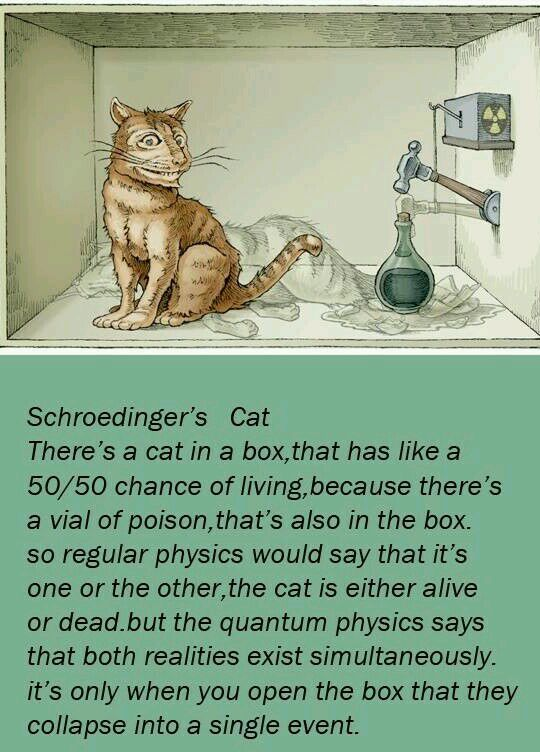
\includegraphics[height=0.70\textwidth,width=0.48\textwidth,viewport=0 0 550 750,clip]{Figures/Schrodinger-cat.jpg}
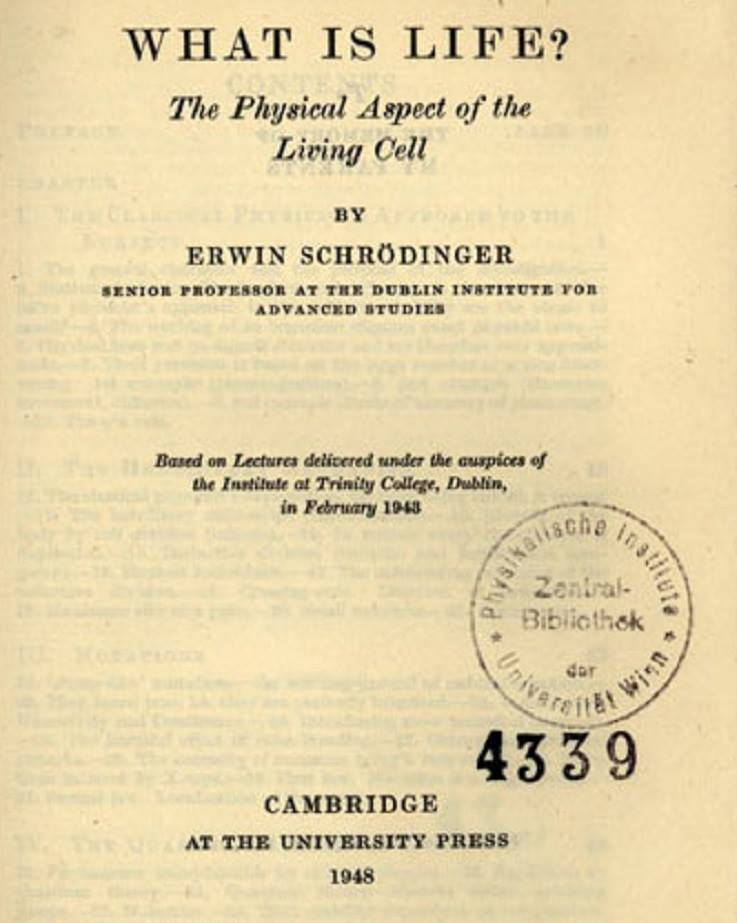
\includegraphics[height=0.70\textwidth,width=0.50\textwidth,viewport=0 0 720 930,clip]{Figures/Schrodinger_book.jpg}
%\caption{\textrm{ABINIT}的Si.in}
\label{Schrodinger-cat}
\end{figure}
}

\frame
{
	\frametitle{因果倒置:~\textrm{Delayed Choice Experiment}}
\begin{figure}[h!]
\centering
\vspace{-10.5pt}
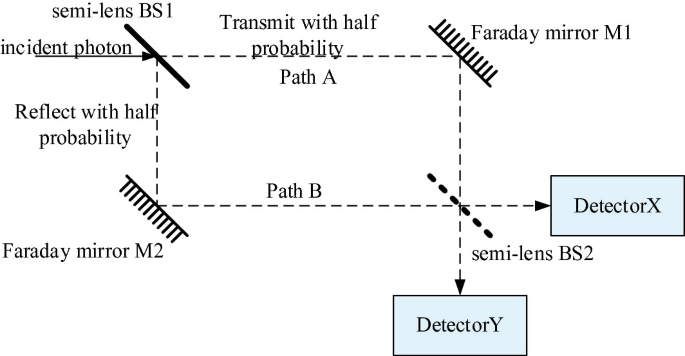
\includegraphics[height=0.55\textwidth,width=1.0\textwidth,viewport=0 0 690 370,clip]{Figures/Schematic-diagram-of-delayed_choice-experiment.png}
\caption{\fontsize{5.2pt}{3.9pt}\selectfont{\textrm{Schematic diagram of delayed choice experiment with A Mach-Zehnder Interferometer.}}}
\label{Delayed_Choice-Experiment}
\end{figure}
}

\frame
{
	\frametitle{量子力学量力学}
\begin{figure}[h!]
\centering
\vspace{-13.5pt}
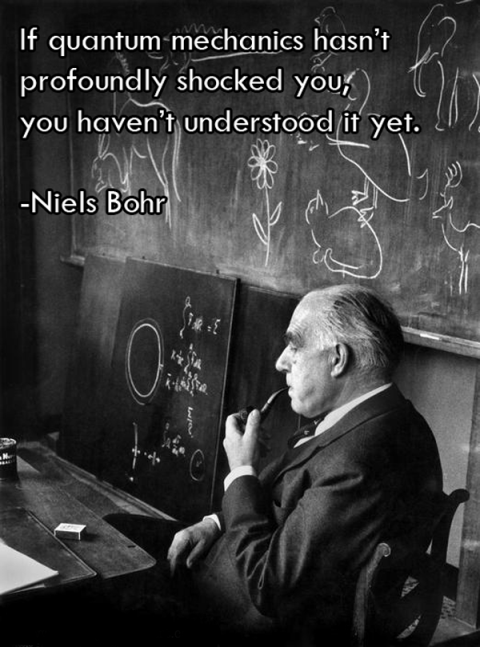
\includegraphics[height=0.75\textwidth,width=0.55\textwidth,viewport=0 0 500 650,clip]{Figures/Quote-Niels_Bohr-on-Quantum_mechanics.png}
\caption{\fontsize{5.2pt}{3.9pt}\selectfont{\textrm{A quote of Niels Bohr on Quantum mechanics.}}}
\label{Quote-Niels_Bohr}
\end{figure}
}

\frame
{
	\frametitle{几何原本:~公理体系的源头}
\begin{figure}[h!]
\centering
\vspace{-13pt}
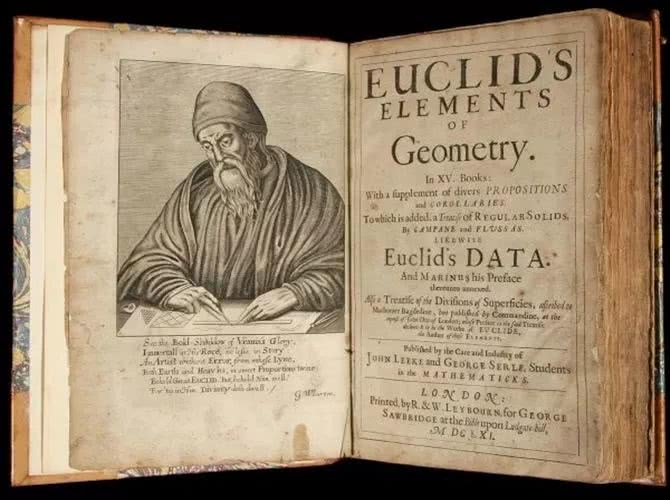
\includegraphics[height=0.38\textwidth,width=0.65\textwidth,viewport=0 0 680 500,clip]{Figures/Element_Geometry_1.jpg}\\
\vspace{1pt}
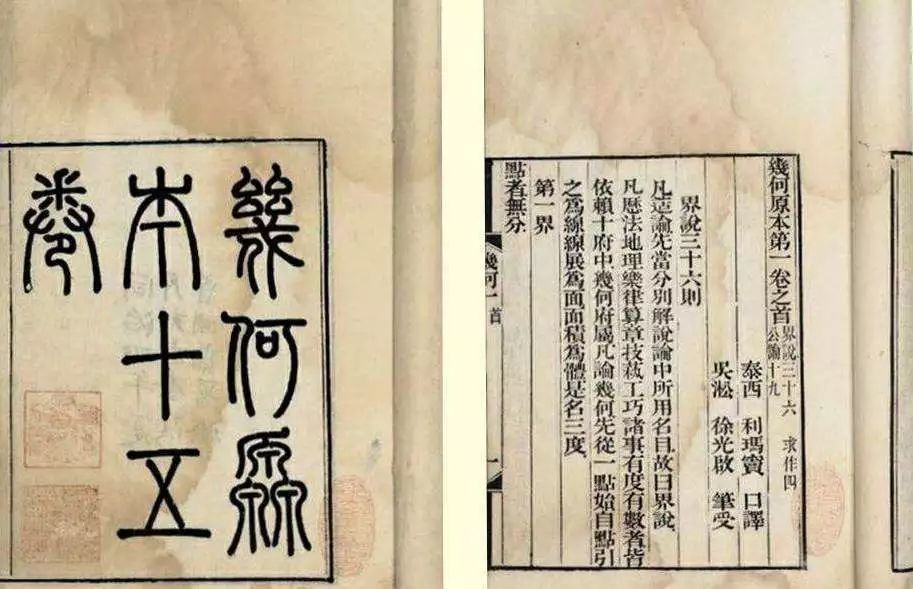
\includegraphics[height=0.36\textwidth,width=0.65\textwidth,viewport=0 0 810 500,clip]{Figures/Element_Geometry_2.jpg}
%\caption{\textrm{ABINIT}的Si.in}
\label{Element_Geometru}
\end{figure}
}

\frame
{
	\frametitle{\textcolor{red}{公理体系}:~现代科学的逻辑起点}
\begin{figure}[h!]
\centering
\vspace{-10.5pt}
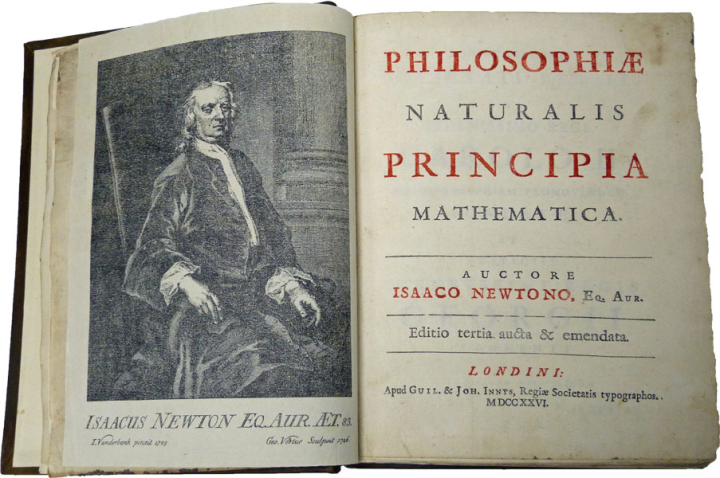
\includegraphics[height=0.68\textwidth,width=1.0\textwidth,viewport=0 0 770 500,clip]{Figures/Philp_Nature_Mach-2.png}
%\caption{\textrm{ABINIT}的Si.in}
\label{Philp_Nature}
\end{figure}
}

\frame[allowframebreaks]
{
	\frametitle{量子力学基本假设(\textcolor{red}{公理体系})}
	\begin{itemize}
		\item 全同粒子假设\\
			\textcolor{blue}{全同粒子组成的体系中,两个全同粒子相互调换不改变体系的状态}\\ 
			全同粒子是指\textcolor{red}{内禀性质完全相同的一类微观粒子}:\\例如,所有的电子是全同粒子 
		\item 波函数假设\\
			\textcolor{blue}{微观体系的运动状态可由波函数$\Psi$完全描述,波函数包含体系的所有性质}\\
			波函数$\Psi$一般要求满足\textcolor{red}{连续}、\textcolor{red}{有限}和\textcolor{red}{单值}三个条件
		\item 微观体系的运动状态\textcolor{blue}{波函数随时间变化的规律}:\\\textcolor{red}{遵从\textrm{Schr\"odinger}方程}
			$$\mathrm{i}\hbar\dfrac{\mathrm{d}}{\mathrm{d}t}|\Psi\rangle=\hat{\mathbf H}|\Psi\rangle$$
		\item 态叠加原理\\
			如果$\Psi_1$是体系的一个本征态,对应的本征值为$A_1$,$\Psi_2$也是体系的一个本征态,对应的本征值为$A_2$,则\textcolor{blue}{$$\Psi=C_1\Psi_1+C_2\Psi_2$$}\textcolor{red}{也是体系一个可能的存在状态}
		\item 力学量算符假设\\
			\textcolor{blue}{经典力学的物理量对应到量子力学中,要用线性~\textrm{Hermite}算符表示}(\textcolor{red}{\textrm{Hermite~}算符的本征函数构成完备空间})\\
			如动量算符 ~~~ $\hat{\mathbf{p}}=-\mathrm{i}\hbar\nabla$\\
			~~~位置算符 ~~~ $\hat{\mathbf r}=r$\\
			力学量算符之间有确定的对易关系(\textcolor{brown}{量子条件})
			$$[\hat{\mathbf F},\hat{\mathbf G}]=\hat{\mathbf F}\hat{\mathbf G}-\hat{\mathbf G}\hat{\mathbf F}$$ 
			
	\end{itemize}
}

\frame
{
	\frametitle{叠加态的数学表示:~矩阵}
\begin{figure}[h!]
\centering
\vspace{-1.5pt}
\hspace*{-0.12in}
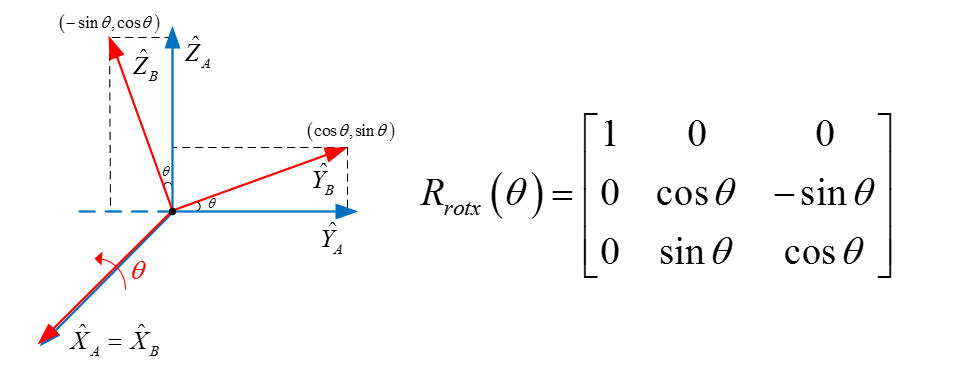
\includegraphics[height=0.48\textwidth,width=1.05\textwidth]{Figures/Matrix_Rotation.png}
%\caption{\textrm{ABINIT}的Si.in}
\label{Matrix-Rotation}
\end{figure}
}

\frame
{
	\frametitle{量子化学学科创立}
	\begin{itemize}
		\item \textrm{1927}年,\textrm{\o.~Burrau}应用量子力学原理,完成\textrm{\ch{H2+}}离子的计算
		\item 同年,\textrm{Walter~Heitlery}和\textrm{Fritz~W.~London}对\textrm{\ch{H2}}分子的计算,标志着量子化学这一学科正式创立
	\end{itemize}
\begin{figure}[h!]
\centering
\vspace{-1.5pt}
\hspace*{-0.12in}
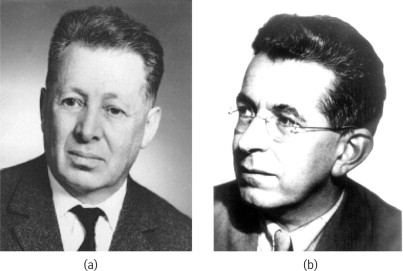
\includegraphics[height=0.48\textwidth,width=0.80\textwidth,viewport=0 10 260 175,clip]{Figures/Walter-Heitlery_Fritz-W-London.jpeg}
\caption{\textrm{W.~Heitlery (left) and F.~W.~London(right).}}
\label{Heitlery_London}
\end{figure}
}

%\frame
%{
%	\frametitle{\textrm{Paul Adrian Maurice Dirac's Commandments}}
%	\textrm{The underlying laws necessary for the mathematical treatment of a large part of physics \textcolor{red}{and the whole of chemistry} are thus completely known, and the difficulty lies only in the fact that application of these laws leads to equations that are \underline{too complex to be solved}.
%\vskip 15pt
%It therefore becomes desirable that approximation practical methods of applying quantum mechanics should be develop $\cdots$ 
%}

%\vskip 15pt
%\textrm{P.A.M Dirac Proc. Roy. Soc. Ser. A, \textbf{123}, 714, (1929)}
%}
%
\frame
{
%	\frametitle{\rm{Paul Dirac's Commandments\upcite{PRSLSA123-714_1929}}}
	\frametitle{\textrm{Paul Dirac's Commandments}}%\upcite{PRSLSA123-714_1929}}}
%	\textrm{\textcolor{purple}{The underlying laws necessary for the mathematical treatment of a large part of physics and the whole of chemistry are thus completely known, and the difficulty lies only in the fact that application of these laws leads to equations that are too complex to be solved.}}
\begin{figure}[h!]
\centering
\vspace{-10.5pt}
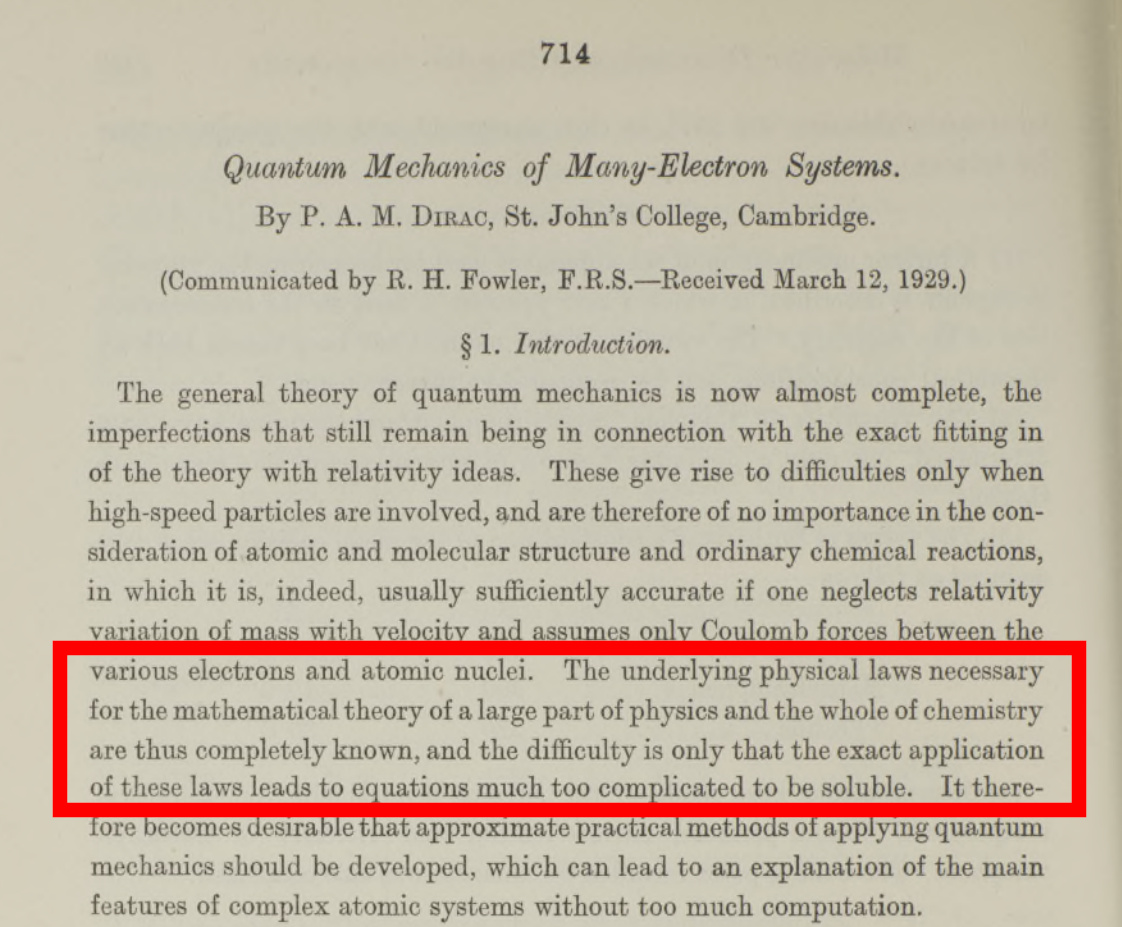
\includegraphics[height=0.71\textwidth,width=0.9\textwidth,viewport=0 0 1150 920,clip]{Figures/Dirac_comment.png}
%\caption{\textrm{ABINIT}的Si.in}
\label{Diract_Commandment}
\end{figure}
}

%-----------------------------------------------------------------------------
\section{{\rm{Hartree-Fock}}~方法}
\frame
{
	\frametitle{\textrm{Born-Oppenheimer~}近似}
	\begin{itemize}
		\item 由于原子核的质量要比电子大很多(一般要大3-4个数量级),在同样的相互作用下,原子核的运动比电子也慢得多
		\item 电子在每一时刻仿佛运动在静止原子核构成的势场中,而原子核运动时则感受不到电子的具体位置,感受到的是运动电子的平均作用力
		\item 可近似将原子核坐标与电子坐标变量分离,使得求解整个体系的波函数的复杂过程分解为求解电子波函数和求解原子核波函数两个相对简单的过程\\
			电子运动方程$$\hat{\mathbf H}_{\mathrm e}(\vec r,\vec{\mathbf R})\Psi(\vec r,\vec{\mathbf R})=E_{\mathrm e}(\vec{\mathbf R})\Psi(\vec r,\vec{\mathbf R})$$
			原子核运动方程$$[\hat{\mathbf T}_{\mathrm{nul}}+E_{\mathrm e}(\vec{\mathbf R})]\chi(\vec{\mathbf R})=E\chi(\vec{\mathbf R})$$
	\end{itemize}
}

\frame
{
	\frametitle{独立粒子近似}
	\textrm{n-}粒子体系中的每个粒子的运动,完全忽略粒子间的瞬时相互作用,认为第$i$个粒子在其余$\mathrm{n}-1$个粒子组成的平均势场中运动
	$$\Psi(\vec r_1,\vec r_2,\vec r_3,\cdots,\vec r_n)=\psi_1(\vec r_1)\psi_2(\vec r_2)\psi_3(\vec r_3)\cdots\psi_n(\vec r_n)$$
	$$\hat{\mathbf H}=\sum_{i=1}^N-\dfrac{1}{2}\nabla_i^2+\sum_{i=1}^NV_i(\vec r_i)+\sum_{i,j(j\neq i)}\dfrac{e^2}{|\vec r_i-\vec r_j|}$$
	粒子$i$的\textrm{Hartree}算符
	$$\hat{\mathbf h}_i=-\dfrac{1}{2}\nabla_i^2+V_i(r_i)+\sum_{j(j\neq i)}^N\dfrac{e^2}{|\vec r_i-\vec r_j|}$$
	因此每个粒子的运动方程为:
	$$\hat{\mathbf h}_i\psi_i(\vec r)=\bigg[-\dfrac{1}{2}\nabla_i^2+V_i(r_i)+\sum_{j(j\neq i)}^N\dfrac{e^2}{|\vec r_i-\vec r_j|}\bigg]\psi_i(\vec r)=\varepsilon\psi_i(\vec r)$$ 
}

\frame
{
	\frametitle{\textrm{Slater~}行列式}
	简单乘积的独立粒子波函数不满足全同粒子置换对称性要求,不能正确表示电子不可辨认的物理属性
	
	\textrm{Slater}建议用行列式形式表示具有反对称性的波函数
	\begin{displaymath}
		\hspace*{-10pt}\Psi(\vec r_1,\vec r_2,\vec r_3,\cdots,\vec r_n)=\dfrac1{\sqrt{n!}}
		\left|\begin{array}{ccccc}
			\psi_1(\vec r_1)&\psi_2(\vec r_1)&\psi_3(\vec r_1)&\cdots&\psi_n(\vec r_1)\\
			\psi_1(\vec r_2)&\psi_2(\vec r_2)&\psi_3(\vec r_2)&\cdots&\psi_n(\vec r_2)\\
			\psi_1(\vec r_3)&\psi_2(\vec r_3)&\psi_3(\vec r_3)&\cdots&\psi_n(\vec r_3)\\
			&&&\cdots&\\
			\psi_1(\vec r_n)&\psi_2(\vec r_n)&\psi_3(\vec r_n)&\cdots&\psi_n(\vec r_n)
		\end{array}\right|
	\end{displaymath}
	粒子$i$的\textrm{Fock}算符
	$$\hat{\mathbf F}_i=-\dfrac{1}{2}\nabla_i^2+V_i(r_i)+\hat{\mathbf J}_i-\hat{\mathbf K}_i$$
	$$\hat{\mathbf J}_i(\vec r_i)=\int\dfrac{\psi_j^{\ast}(\vec r_j)|e^2|\psi_j(\vec r_j)}{|\vec r_i-\vec r_j|}\mathrm{d}\vec r_j$$
	$$\hat{\mathbf K}_i(\vec r_i)\psi_i(\vec r_i)=\psi_j(\vec r_i)\int\dfrac{\psi_j(\vec r_j)|e^2|\psi_i(\vec r_j)}{|\vec r_i-\vec r_j|}\mathrm{d}\vec r_j$$

}

\frame
{
	\frametitle{\textrm{Hartree-Fock-Roothan~}方法}
	实际求解非相对论的\textrm{Schr\"odinger}方程时,
	$$\hat{\mathbf F}_i\psi_i(\vec r_i)=\varepsilon_i\psi_i(\vec r_i)$$
	将波函数$\psi_i(\vec r_i)$用一套选定的基函数$\phi_j(\vec r)$展开
	$$\psi_i(\vec r)=\sum_{j=1}^Nc_{ij}\phi_j(\vec r)$$
	通过变分原理
	$$\bar E=\dfrac{\langle\Psi|\hat{\mathbf H}|\Psi\rangle}{\langle\Psi|\Psi\rangle}\geqslant E_0$$
	改变展开系数$c_{ij}$直到体系的能量最小,确定展开系数

	重复上述流程直至\textrm{Fock}算符$\hat{\mathbf F}$、波函数$\psi(\vec r)$和能量$\varepsilon$自洽,这就是\textrm{Hartree-Fock-Roothan}方法
}

\frame
{
	\frametitle{\textrm{Slater~}的$\chi_{\alpha}$方法}
	由于\textrm{Hartree-Fock~}的交换势计算复杂,\textrm{Slater~}建议用电子密度的加权平均来简化交换势的求解
	\begin{displaymath}
		V_{\mathrm x}=-\frac{\sum\limits_i\sum\limits_jn_in_j\int\varphi_i^{\ast}(\vec r)\varphi_i(\vec r{}^{\prime})(2/|\vec r-\vec r{}^{\prime}|)\varphi_j^{\ast}(\vec r{}^{\prime})\varphi_j(\vec r)\mathrm{d}\vec r}{\sum\limits_kn_k\varphi_k^{\ast}(\vec r)\varphi_k(\vec r)}
	\end{displaymath}
	自由电子气在动量空间用\textrm{Hartree-Fock}方法表示
	\begin{displaymath}
		V_{\mathrm x}(k)=-8\left( \frac3{8\pi}\rho \right)^{1/3}F(\eta)
	\end{displaymath}
	这里$\eta=k/k_{\mathrm F}$,并有
	\begin{displaymath}
		F(\eta)=\frac12+\frac{1-\eta^2}{4\eta}\ln\left|\frac{1+\eta}{1-\eta}\right|
	\end{displaymath}
	$F(\eta)$在$\eta=1(k=k_{\mathrm F})$出现奇点(对应于自由电子气\textrm{Fermi~}面上电子密度为0)。
}
	
\frame
{
	\frametitle{\textrm{Slater~}的$\chi_{\alpha}$方法}
	\textrm{Slater~}建议,对占据态($k\leqslant k_{\mathrm F}$)的电子作加权平均,可有
	\begin{displaymath}
		F(\eta)=\frac{\int_0^1\eta^2F(\eta)\mathrm{d}\eta}{\int_0^1\eta^2\mathrm{d}\eta}=\frac34
	\end{displaymath}
	因此,对于均匀电子气,交换势
	\begin{displaymath}
		V_{\mathrm x}=-6\left( \frac3{8\pi}\rho \right)^{1/3}
	\end{displaymath}
	\textrm{Slater~}指出,对于局域电子密度$\rho(\vec r)$体系,可有\textrm{Slater~}交换势
	\begin{displaymath}
		V_{\mathrm xs}(\vec r)=-6\left( \frac3{8\pi}\rho(\vec r) \right)^{1/3}
	\end{displaymath}
	在此基础上,\textrm{Slater~}建议对上述交换势引入可调参数$\alpha$,有交换势
	\begin{displaymath}
		V_{\chi_{\alpha}}(\vec r)=\alpha V_{\mathrm xs}(\vec r)
	\end{displaymath}
}

\frame
{
	\frametitle{交换与相关}
	\begin{itemize}
		\item \textrm{Fock}算符中的交换算符$\hat{\mathrm K}_i(\vec r_i)$是由\textrm{Slater}行列式引入的,属于量子效应
	\end{itemize}
%	\vspace*{-5pt}
	\begin{displaymath}
%		\hspace*{-2pt}
		\text{电子间瞬时相互作用(\textcolor{red}{关联})}
		\left\{
			\begin{aligned}
				&\text{\textcolor{blue}{电子交换}:同自旋电子的关联作用}\\
				&\text{\textcolor{blue}{电子相关}}
			\end{aligned}
			\right.
	\end{displaymath}
\begin{figure}[h!]
\centering
\vspace{-10.5pt}
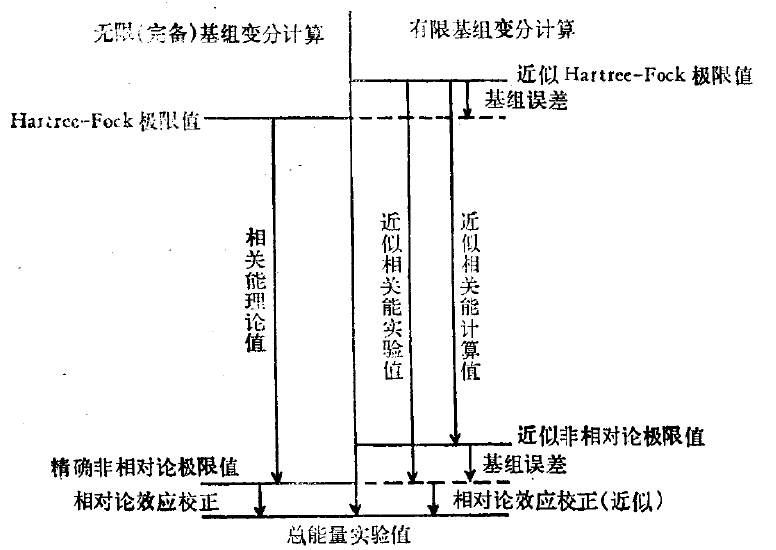
\includegraphics[height=0.42\textwidth,width=0.6\textwidth,viewport=0 0 760 550,clip]{Figures/Post-HF.png}
%\caption{\textrm{ABINIT}的Si.in}
\label{Post-HF}
\end{figure}
}

\frame
{
	\frametitle{\textrm{Post-HF}}
	\textrm{Hartree-Fock}方法精确定义了交换作用,完全没考虑电子相关作用
	\begin{itemize}
		\item \textrm{CI (Configuration Interaction)}
	$$\Psi=\sum_{I=0}C_I\Phi_I=C_0\Phi_0+C_1\Phi_1+C_2\Phi_2+\cdots$$
		\item \textrm{CC (Couple Cluste)}\\
			\begin{displaymath}
				\Psi=\mathrm{e}^{\hat{\mathbf T}}\Phi_0=\mathrm{e}^{(\hat{\mathbf T}_1+\hat{\mathbf T}_2+\hat{\mathbf T}_3+\cdots)}\Phi_0
			\end{displaymath}
		\item \textrm{MP}微扰方法
			\begin{displaymath}
				\begin{aligned}
					&\hat{\mathbf H}=\hat{\mathbf H}^{(0)}+\hat{\mathbf V} \\
					&\hat{\mathbf H}^{(0)}=\sum_i\hat{\mathbf F}_i \qquad \Phi^{(0)}=\Psi_{\mathrm{HF}}\\ 
					&\hat{\mathbf V}=\sum_{j>i}^{\mathrm occ}\dfrac{e^2}{r_{ij}}-\sum_{ij}^{\mathrm occ}\big(\hat{\mathbf J}_{ij}-\dfrac12\hat{\mathbf K}_{ij}\big)
				\end{aligned}
			\end{displaymath}
	\end{itemize}
}

\section{密度泛函理论}       %Bookmark
\subsection{{\rm{Thomas-Fermi~}}模型}       %Bookmark
\frame
{
	\frametitle{{\textrm{Thomas-Fermi}}模型} 
	\textrm{1927}年,\textrm{Thomas}和\textrm{Fermi}基于均匀电子气模型上建立\textrm{Thomas-Fermi}模型,\textcolor{blue}{体系能量可用}\textcolor{red}{电子密度}\textcolor{blue}{表示}:
	\begin{itemize}
		\item 动能表达式
			$$T_{\mathrm{TF}}[\rho(\vec r)]=\dfrac3{10}(3\pi^2)^{\frac23}\int\rho^{\frac53}(\vec r)\mathrm{d}\vec r$$
		\item 外势$V_{ext}(\vec r)$下电子体系的能量泛函表达式为
			\begin{displaymath}
				\begin{aligned}
					E_{\mathrm{TF}}[\rho(\vec r)]=&\dfrac3{10}(3\pi^2)^{\frac23}\int\rho^{\frac53}(\vec r)\mathrm{d}\vec r\\
					&+\int\rho(\vec r)V_{ext}(\vec r)\mathrm{d}\vec r+\dfrac12\int\int\dfrac{\rho(\vec r_1)\rho(\vec r_2)}{|\vec r_2-\vec r_1|}\mathrm{d}\vec r_1\mathrm{d}\vec r_2
				\end{aligned}
			\end{displaymath}
		\item \textrm{Thomas-Fermi}模型完全没有考虑电子的交换-相关作用
	\end{itemize}
}

\frame
{
	\frametitle{{\textrm{Thomas-Fermi-Dirac}}模型} 
	1930年,\textrm{Dirac}将\textrm{Thomas-Fermi}模型修正,用局域密度近似考虑电子交换作用
			\begin{displaymath}
				\begin{aligned}
					E_{\mathrm{TFD}}[\rho(\vec r)]=&\dfrac3{10}(3\pi^2)^{\frac23}\int\rho^{\frac53}(\vec r)\mathrm{d}\vec r+\int\rho(\vec r)V_{ext}(\vec r)\mathrm{d}\vec r\\
					&+\dfrac12\int\int\dfrac{\rho(\vec r_1)\rho(\vec r_2)}{|\vec r_2-\vec r_1|}\mathrm{d}\vec r_1\mathrm{d}\vec r_2-\dfrac34\bigg(\dfrac3{\pi}\bigg)^{\frac13}\int\rho^{\frac43}(\vec r)\mathrm{d}\vec r
				\end{aligned}
			\end{displaymath}
			\begin{itemize}
				\item 在总电子数守恒约束条件
					$$\int\rho(\vec r)\mathrm{d}\vec r=N$$
					下,能量泛函$E_{\mathrm{TFD}}[\rho(\vec r)]$对密度$\rho(\vec r)$的变分极小获得体系的基态密度和基态能量
			\end{itemize}
}

\frame
{
	\frametitle{\textrm{Thomas-Fermi}模型}
	\begin{itemize}
		\item \textrm{Thomas-Fermi}模型用电子密度代替波函数描述问题是极大的简化,但模型过于粗糙:\\
%			\begin{enumerate}
%				\item 以均匀电子气的密度得到动能的表达式
%				\item 完全忽略电子间的交换-相关作用
%			\end{enumerate}
			不能正确描述相互作用电子体系的基本特征,如原子的壳层结构
		\item \textrm{Thomas-Fermi}模型虽不够精确,但可以通过引入修正项校正:
			\textrm{Dirac}交换泛函 $$E_X[\rho(\vec r)]=-\dfrac34\bigg(\dfrac3{\pi}\bigg)^{\frac13}\int\rho^{\frac43}(\vec r)\mathrm{d}\vec r$$
			\textrm{Wigner}相关泛函 $$E_C[\rho(\vec r)]=-0.056\int\dfrac{\rho^{\frac43}(\vec r)}{0.079+\rho^{\frac13}(\vec r)}\mathrm{d}\vec r$$
	\end{itemize}
	\textrm{Thomas-Fermi}模型为密度泛函理论\textrm{(DFT)}提供了重要的启示
}

\subsection{密度泛函理论}       %Bookmark
\frame                               %
{
\frametitle{密度泛函理论(\textrm{DFT})} %Slide Page Title
%   \secname
与传统的量子力学方法不同,密度泛函理论的基本变量是体系的基态电子密度。%通过体系的电子密度而非波函数确定体系的基态能量。
\begin{itemize}%[+-| alert@+>]
	\item 密度泛函理论的基石:\textrm{Hohenberg-Kohn}定理\upcite{PR136-B864_1964}
\vskip 5pt
\begin{itemize}%[+-| alert@+>]
   \setlength{\itemsep}{8pt}
 \item $E[\rho]=F_{\mathrm{HK}}[\rho]+\displaystyle\int\rho(\vec{r})v(\vec{r})\textrm{d}\vec{r}$ \\
\vskip 5pt 
{\fontsize{7.2pt}{6.2pt}\selectfont{其中$F_{\mathrm{HK}}[\rho]=\underset{\Psi\to\rho}{\mathrm{Min}}\langle\Psi[\rho]|\hat{T}+\hat{W}|\Psi[\rho]\rangle$
是普适的泛函表达式}}\\%,指明多电子体系的基态性质与基态密度间存在一一对应关系
\textcolor{magenta}{\fontsize{8.2pt}{6.2pt}\selectfont{第一定理表明多电子体系的性质完全由体系的基态密度决定}}
   \item 如果$\tilde\Psi\neq\Psi$,
     $E[\tilde\rho]\geqslant E[\rho_0]$\\
     \textcolor{magenta}{\fontsize{8.2pt}{6.2pt}\selectfont{第二定理指出基态总能量泛函在体系基态电子密度处取极小值}}
   \end{itemize}
\vskip 8pt
 \item 密度泛函理论的优越性:~用密度($\rho$)代替波函数($\Psi$)描述体系
\vskip 5pt
 \item 密度泛函理论的困难:~能量密度泛函的精确形式未知
   \end{itemize}
}

\frame
{
	\frametitle{\rm{Creators of DFT}}
\begin{figure}[h!]
\vskip 10pt
\centering
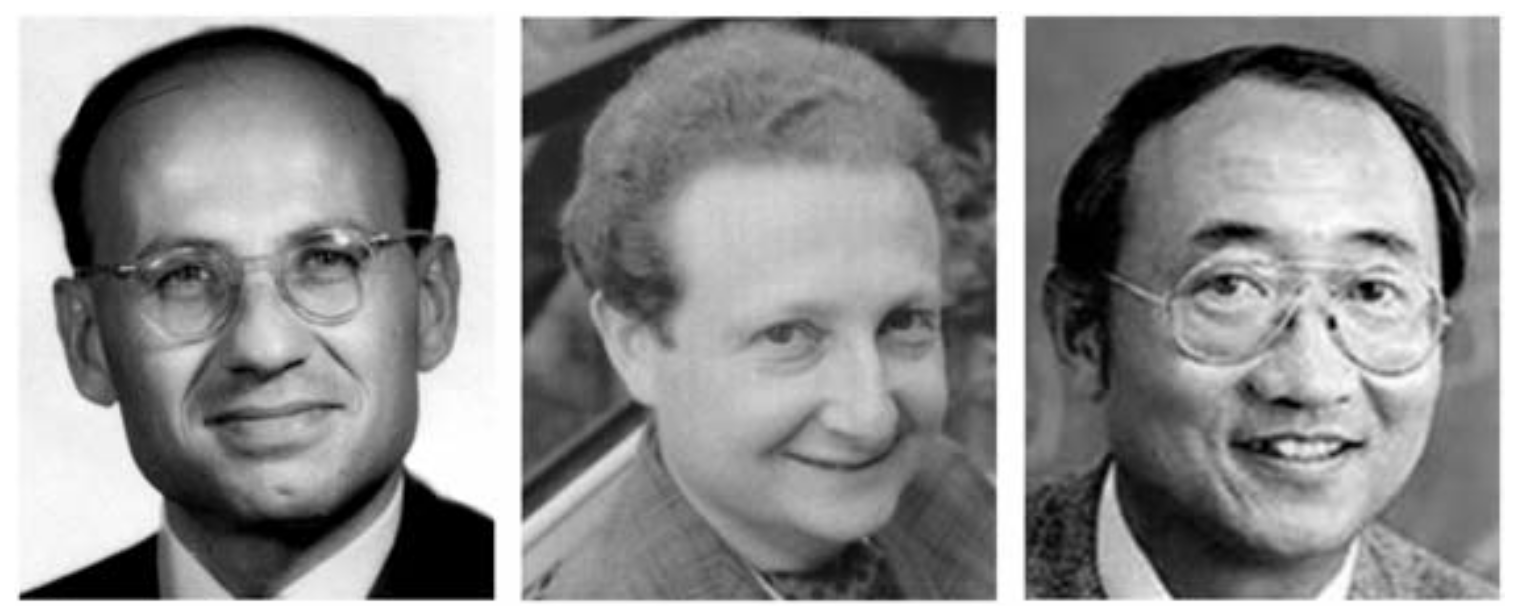
\includegraphics[height=1.65in,width=4.0in,viewport=0 0 1562 610,clip]{Figures/Creators_of_DFT.png}
\caption{\tiny \textrm{Creators of DFT. Walter Kohn(left, in 1962) and his two postdoctoral fellows, Pierre Hohenberg (middle, in 1965) and Lujeu Sham (right).}}%(与文献\cite{EPJB33-47_2003}图1对比)
\label{Creator_of_DFT}
\end{figure}
}

\frame                               %
{
\frametitle{密度泛函理论(\textrm{DFT})}
\textrm{Kohn-Sham}方程\upcite{PR140-A1133_1965}:无相互作用体系+交换-相关能的贡献
$$(T_S+V_{e\!f\!f})|\varphi_i\rangle=\varepsilon_i|\varphi_i\rangle,\quad i=1,\cdots,N,\cdots$$
其中$T_S=-\dfrac12\nabla^2$~~是无相互作用体系的动能
\begin{displaymath}
	\begin{aligned}
		V_{e\!f\!f}(\vec r)=&V_{ext}(\vec r)+\displaystyle\int w(\vec r,\vec r\,')\rho(\vec r\,')\mathrm{d}\vec r\,'+V_{\mathrm{XC}}[\rho]\\
=&\displaystyle\int\dfrac{\rho(\vec r\,')}{|\vec r-\vec r^{\prime}|}\mathrm{d}\vec r\,'+V_{ext}(\vec r)+V_{\mathrm{XC}}[\rho]
	\end{aligned}
\end{displaymath}
$V_{ext}(\vec r)$是电子体系与外部的电荷或磁场相互作用\\
$V_{\mathrm{XC}}[\rho]=\dfrac{\delta E_{\mathrm{XC}}}{\delta\rho(\vec r)}$称为交换-相关势
\vskip 10pt
\textrm{Kohn-Sham}方程是形式上的单粒子方程
\vskip 6pt
\textrm{Kohn-Sham}方程的实质:\\\textcolor{red}{将动能泛函的主要部分分离出来,剩余部分放在交换-相关能中}
}

\frame{
\begin{figure}[h!]
\vskip -10pt
\centering
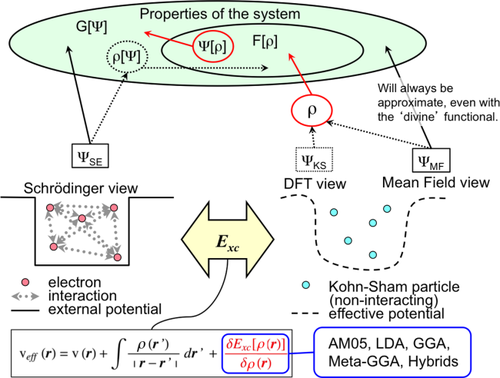
\includegraphics[height=2.65in,width=3.8in,viewport=0 0 362 275,clip]{Figures/DFT-particle-density.png}
\caption{\fontsize{6.0pt}{4.5pt}\selectfont{\textrm{Properties of a quantum mechanical system can be calculated by solving the SE (left). A more tractable, formally equivalent way is to solve the DFT KS equations (right).}}}%(与文献\cite{EPJB33-47_2003}图1对比)
\label{Schrodinger-equation-vs-Kohn-Sham-equation}
\end{figure}
}

\frame
{
\frametitle{交换-相关能与交换-相关势}
实际考虑交换-相关能时,会将交换-相关能表示为交换能和相关能之和:
\begin{displaymath}
	E_{\mathrm{XC}}[\rho]=E_{\mathrm{X}}[\rho]+E_{\mathrm{C}}[\rho]=\int\varepsilon_{\mathrm{X}}[\rho]\rho(\vec{r}) \textrm{d}^3\vec{r}+\int\varepsilon_{\mathrm{C}}[\rho]\rho(\vec{r}) \textrm{d}^3\vec{r}
\end{displaymath}
$\varepsilon_{\mathrm{X}}[\rho]$和$\varepsilon_{\mathrm{C}}[\rho]$可理解为单电子的交换能和相关能
\vskip 20pt
交换-相关势通过交换-相关能计算得到:~
		\begin{displaymath}
			V_{\mathrm{XC}}^{\sigma}[\rho_{\alpha},\rho_{\beta}]=\dfrac{\delta E_{\mathrm{XC}}[\rho_{\alpha},\rho_{\beta}]}{\delta\rho_{\sigma}}=\dfrac{\delta\{E_{\mathrm{X}}[\rho_{\alpha},\rho_{\beta}]+E_{\mathrm{C}}[\rho_{\alpha},\rho_{\beta}]\}}{\delta\rho_{\sigma}}
		\end{displaymath}
		\textcolor{red}{注意}:~由于$E_{\mathrm{XC}}[\rho_{\sigma}]$对$\rho_{\sigma}$是非线性的\\
		\textcolor{blue}{$V_{\mathrm{XC}}=V_{\mathrm{X}}+V_{\mathrm{C}}$和$\varepsilon_{\mathrm{XC}}=\varepsilon_{\mathrm{X}}+\varepsilon_{\mathrm{C}}$不同,不要混淆这两个量}
}
%  \beamertemplateshadingbackground{blue!10}{yellow!10}

\frame                               %
{
\frametitle{交换-相关能密度泛函}
\textcolor{blue}{密度泛函理论的核心问题}:\\
\textrm{Kohn-Sham}方程用于实际计算,必须知道$E_{\textrm{XC}}[\rho]$或者$V_{\textrm{XC}}[\rho]$与$\rho(\vec r)$的泛函关系
\vskip 15pt
\begin{minipage}[b]{0.59\textwidth}
 \hspace*{-15pt}
 {\fontsize{7.5pt}{6.0pt}\selectfont\begin{itemize}%[+-| alert@+>]
	 \setlength{\itemsep}{15pt}
 \item \textrm{LDA}:泛函只与密度分布的局域值有关
 \item \textrm{GGA}:泛函依赖:局域密度及其梯度
 \item $meta$-\textrm{GGA}:泛函依赖的变量还有动能密度
 \item 杂化(\textrm{hybrid})泛函:泛函与占据轨道有关
 \item 其他的交换-相关能泛函
 \item<1-> 完全非局域泛函:理想泛函,不现实
 \end{itemize}}
\end{minipage}
\hfill
\begin{minipage}[b]{0.39\textwidth}
\hspace*{-10pt}
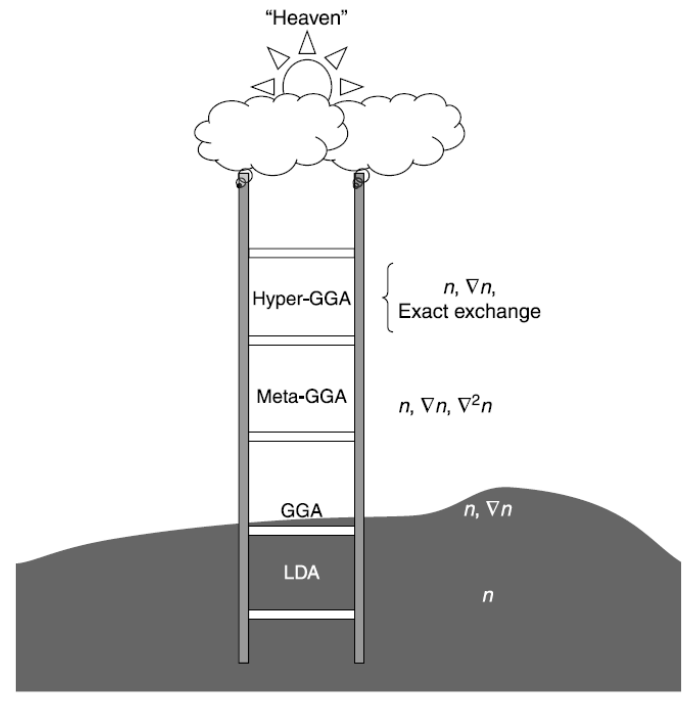
\includegraphics[height=1.7in,width=3.18in,viewport=10 5 1380 700,clip]{Figures/Jacobi-ladder.png}\\
\centering{\textcolor{red}{\textrm{\tiny Jacob's ladder}}}
\end{minipage}
% \begin{itemize}%[+-| alert@+>]
%\item 交换-相关能密度泛函
}

\subsection{常见泛函的一些形式}
\frame%[allowframebreaks]
{
	\frametitle{\rm{LDA}泛函}
	\begin{itemize}
		\item 交换能部分
	\begin{displaymath}
		\begin{aligned}
			\varepsilon_{\mathrm{X}}[\rho,\zeta]=&2^{-1/3}C_{\mathrm{X}}^{\sigma}g(\zeta)\rho^{1/3}(\vec r)\\
			E_{\mathrm{X}}[\rho,\zeta]=&\int\varepsilon_{\mathrm{X}}[\rho,\zeta]\rho(\vec r)\mathrm{d}\vec r\\
		\end{aligned}
	\end{displaymath}
	{\fontsize{7.5pt}{6.0pt}\selectfont{这里:~$C_{\mathrm{X}}^{\sigma}=\dfrac32\bigg(\dfrac3{4\pi}\bigg)^{1/3}$\\
		$g(\zeta)=\dfrac12\bigg[(1+\zeta)^{4/3}+(1-\zeta)^{4/3}\bigg]$\\
		$\zeta(\vec r)=\dfrac{[\rho_{\alpha}(\vec r)-\rho_{\beta}(\vec r)]}{[\rho_{\alpha}(\vec r)+\rho_{\beta}(\vec r)]}$}}
	\end{itemize}
}

\frame%[allowframebreaks]
{
	\frametitle{\rm{LDA}泛函}
	\begin{itemize}
		\item 相关能部分
			\begin{displaymath}
				\hspace*{-30pt}	\varepsilon_{\mathrm{C}}^{\mathrm{LDA}}(r_s,\zeta)=\varepsilon_{\mathrm{C}}(r_s,0)+a_{\mathrm{c}}(r_s)\dfrac{f(\zeta)}{f^{\prime\prime}(\zeta)}(1-\zeta^4)+[\varepsilon_{\mathrm{c}}(r_s,1)-\varepsilon_{\mathrm{c}}(r_s,0)]f(\zeta)\zeta^4
			\end{displaymath}
			{\fontsize{7.5pt}{6.0pt}\selectfont{这里:~$r_s=\bigg[\dfrac3{4\pi}(\rho_{\alpha}+\rho_{\beta})^{-1}\bigg]^{1/3}$~$f(\zeta)=[(1+\zeta)^{4/3}+(1-\zeta)^{4/3}-2]/(2^{4/3}-2)$\\
			$\varepsilon_{\mathrm{C}(r_s,0)}$、$\varepsilon_{\mathrm{C}(r_s,1)}$、$a_{\mathrm{C}(r_s)}$由经验公式
			\begin{displaymath}
				\begin{aligned}
					&G(r_s,A,\alpha_1,\beta_1,\beta_2+\beta_3+\beta_4)\\
					=&-2A(1+\alpha_1r_s)\ln\bigg[1+\dfrac1{2A(\beta_1r_s^{1/2}+\beta_2r_s+\beta_2r_s^{3/2}+\beta_1r_s^2)}\bigg]
				\end{aligned}
			\end{displaymath}
		计算。其中$A$、$\alpha_1$、$\beta_1$、$\beta_2$、$\beta_3$、$\beta_4$是参数,通过拟合实验结果确定}}
		\begin{displaymath}
			E_{\mathrm{C}}[\rho]=\int\rho(\vec r)\varepsilon_{\mathrm{C}}(\vec r)\mathrm{d}\vec r
		\end{displaymath}
	\end{itemize}
}

\frame%[allowframebreaks]
{
	\frametitle{\rm{GGA}泛函}
	\begin{itemize}
		\item 交换能泛函:
			\begin{itemize}
				\item \textrm{PW91}
					\begin{displaymath}
						\begin{aligned}
							E_{\mathrm{X}}^{\mathrm{PW91}}[\rho_{\alpha},\rho_{\beta}]=&\dfrac12(E_{\mathrm{X}}^{\mathrm{PW91}}[2\rho_{\alpha}]+E_{\mathrm{X}}^{\mathrm{PW91}}[2\rho_{\beta}])\\
							E_{\mathrm{X}}^{\mathrm{PW91}}[\rho]=&-\dfrac34\bigg(\dfrac3\pi\bigg)^{1/3}\int\rho^{4/3}(\vec r)F(x)\mathrm{d}\vec r
						\end{aligned}
					\end{displaymath}
					\hspace*{-30 pt}{\fontsize{4.5pt}{4.0pt}\selectfont{这里:~$F(x)=\dfrac{1+0.19645(hx)\sinh^{-1}(7.7956hx)+(hx)^2\{0.2743-0.1508\mathrm{exp}[-100(hx)^2]\}}{1+0.19645(hx)\sinh^{-1}(7.7956hx)+0.004(hx)^4}$}\\
					$h=(24\pi^2)^{-1/3}$,~~~$x=|\nabla\rho|\rho^{-4/3}$}
				\item \textrm{PBE}
			\begin{displaymath}
				E_{\mathrm{X}}^{\mathrm{PBE}}[\rho,x]=E_{\mathrm{X}}^{\mathrm{LDA}}[\rho,x]-C_{\mathrm{X}}\int a\bigg(1-\dfrac1{bx^2}\bigg)\rho^{4/3}(\vec r)\mathrm{d}\vec r
			\end{displaymath}
			{\fontsize{4.5pt}{4.0pt}\selectfont{其中:~$C_{\mathrm{X}}=\dfrac34\bigg(\dfrac3\pi\bigg)^{1/3}$\\$a=0.804$,~~~$b=0.273$~是非经验参数}}
			\end{itemize}
	\end{itemize}
}

\frame%[allowframebreaks]
{
	\frametitle{\rm{GGA}泛函}
	\begin{itemize}
		\item 相关能泛函:
			\begin{itemize}
				\item \textrm{PW91}
					\begin{displaymath}
						\begin{aligned}
							E_{\mathrm{C}}^{\mathrm{PW91}}[\rho_{\alpha},\rho_{\beta}]=&\int\mathrm{d}\vec r\rho(\vec r)[\varepsilon_{\mathrm{C}}^{\mathrm{LSDA}}(r_s,\zeta)]+H(t,r_s,\zeta)\\
							H=&H_0+H_1
						\end{aligned}
					\end{displaymath}
					{\fontsize{4.5pt}{4.0pt}\selectfont{这里:~
						\begin{displaymath}
							\begin{aligned}
								H_0=&f^3(\zeta)\dfrac{\beta^2}{2\alpha}\ln\bigg(1+\dfrac{2\alpha}{\beta}\dfrac{t^2+At^4}{1+At^2+A^2t^4}\bigg)\\
								A=&\dfrac{2\alpha}{\beta}\dfrac1{\mathrm{exp[-2\alpha\varepsilon_{\mathrm{C}}^{\mathrm{LDA}}(r_s,\zeta)}/f^3(\zeta)\beta^2]-1}\\
							t=&\dfrac{|\nabla\rho|}{2f(\zeta)k_s\rho}~~~f(\zeta)=\dfrac12\bigg[(1+\zeta)^{2/3}+(1-\zeta)^{2/3}\bigg]\\
							k_s=&[4(3\pi^{-1}\rho)^{1/3}]^{1/2}
							\end{aligned}
						\end{displaymath}
						参数 $\alpha=0.09$,~~~$\beta=\nu C_{\mathrm{C}}(0)$\\
						$\nu=(16/\pi)(3\pi^2)^{1/3}$,~~~$C_{\mathrm{C}}(0)=0.004235$
				}}
			\end{itemize}
	\end{itemize}
}

\frame%[allowframebreaks]
{
	\frametitle{\rm{meta-GGA}泛函}
	\begin{itemize}
		\item 交换能泛函
			\begin{itemize}
				\item \textrm{TPSS}
					\begin{displaymath}
						\begin{aligned}
							E_{\mathrm{X}}^{\mathrm{TPSS}}[\rho]&=\int\mathrm{d}\vec r\rho(\vec r)\varepsilon_{\mathrm{X}}^{\mathrm{LSDA}}(\vec r)F_{\mathrm{X}}^{\mathrm{TPSS}}(p,z)\\
							F_{\mathrm{X}}^{\mathrm{TPSS}}&=1+\kappa-\dfrac{\kappa}{1+x/\kappa}
						\end{aligned}
					\end{displaymath}
{\fontsize{4.5pt}{4.0pt}\selectfont{这里:~
	$\rho(\vec r)=\rho_{\alpha}(\vec r)+\rho_{\beta}({\vec r})$,~~~$\varepsilon_{\mathrm{X}}^{\mathrm{LSDA}}(\vec r)=-\dfrac3{4\pi}[3\pi^2\rho(\vec r)]^{1/3}$
\\
\begin{displaymath}
	\begin{aligned}
		x=&\left\{\bigg[\dfrac{10}{81}+\dfrac{cz^2}{(1+z^2)^2}\bigg]p+\dfrac{146}{2025}\bar{q}_b^2-\dfrac{73}{405}\bar{q}_b\bigg[\dfrac12\bigg(\dfrac35z\bigg)^2+\dfrac12p^2\bigg]^{1/2}\right.\\
		&+\left.\dfrac1{\kappa}\bigg(\dfrac{10}{81}\bigg)^2p^2\dfrac{20e^{1/2}}{81}\bigg(\dfrac35z\bigg)^2+e\mu p^3\right\}(1+e^{1/2}p)^{-2}\\
		p=&\dfrac{|\nabla\rho(\vec r)|^2}{4(3\pi^2)^{2/3}\rho^{8/3}(\vec r)}, ~~~ \bar{q}_b=\dfrac{(9/20)(\alpha-1)}{[1+b\alpha(\alpha-1)]^{1/2}}+2p/3
	\end{aligned}
\end{displaymath}
$z=\tau_w/\tau$,~~~$\tau_w=\dfrac{|\nabla\rho(\vec r)|^2}{8\rho(\vec r)}$,~~~$\tau=\sum\limits_{\sigma}\tau_{\sigma}$\\
$\alpha=(\tau-\tau_w)/\tau_{\mathrm{unif}}=(5p/3)(z^{-1}-1)$,~~~$\tau_{\mathrm{tiff}}=\dfrac3{10}(3\pi^2)^{2/3}[\rho(\vec r)]^{5/3}$
}}
			\end{itemize}
	\end{itemize}
}


\frame%[allowframebreaks]
{
	\frametitle{\rm{meta-GGA}泛函}
	\begin{itemize}
		\item 相关能泛函
			\begin{itemize}
				\item {\textrm{TPSS}}
					\begin{displaymath}
						E_{\mathrm{C}}^{\mathrm{TPSS}}[\rho_{\alpha,\rho_{\beta}}]=\int\mathrm{d}\vec r\rho(\vec r)\varepsilon_{\mathrm{C}}^{\mathrm{TPSS0}}[1+\mathrm{d}\varepsilon_{\mathrm{C}}^{\mathrm{TPSS0}}(\tau_w/\tau)^3]
					\end{displaymath}
{\fontsize{4.5pt}{4.0pt}\selectfont{这里:~
	\begin{displaymath}
		\begin{aligned}
			\varepsilon_{\mathrm{C}}^{\mathrm{TPSS0}}=&\varepsilon_{\mathrm{C}}^{\mathrm{PBE}}(\rho_{\alpha},\rho_{\beta},\nabla\rho_{\alpha},\nabla\rho_{\beta})[1+C(\zeta,\xi)(\tau_w/\tau)^2]\\
			&-\bigg[1+C(\zeta,\xi)(\tau_w/\tau)^2\sum\limits_{\sigma}\dfrac{\rho_{\sigma}(\vec r)}{\rho(\vec r)}\bar{\varepsilon}_{\mathrm{C}}\bigg]\\
			\bar{\varepsilon}_{\mathrm{C}}=&\max[\varepsilon_{\mathrm{C}}^{\mathrm{PBE}}(\rho_{\alpha},0,\nabla\rho_{\alpha},0),\varepsilon_{\mathrm{C}}^{\mathrm{PBE}}(\rho_{\alpha},\rho_{\beta},\nabla\rho_{\alpha},\nabla\rho_{\beta})]\\
			C(\zeta,\xi)=&\dfrac{C(\zeta,0)}{\{1+\xi^2[(1+\zeta)^{-4/3}+(1-\zeta)^{-4/3}]/2\}^4}
		\end{aligned}
	\end{displaymath}
	$\xi=\dfrac{|\nabla\zeta|}{2[3\pi^2\rho(\vec r)]^{1/3}}$, ~~~$C(\zeta,0)=0.53+0.87\zeta^2+0.50\zeta^4+2.26\zeta^6$
}}
			\end{itemize}
	\end{itemize}
	\vskip 5pt
	\textrm{TPSS}泛函的特点:~\\
	\vskip 3pt
	{\fontsize{7.5pt}{6.0pt}\selectfont{不包含依靠实验数据的可调参数,数字系数由精确能量泛函满足的条件确定\\
		\textcolor{blue}{对电子分布较为均匀的晶体体系和电子分布激烈变化的分子体系都有较高的精度} }}
}

\frame
{
	\frametitle{\rm{hybrid}泛函}
	体系\textrm{Hamilton}算符表示为
	\begin{displaymath}
		\hat{H}_{\lambda}=-\dfrac12\sum_i^N\nabla^2+\sum_i^NV_i(\rho,\lambda)+\dfrac{\lambda}2\sum_i^N\sum_{j(j\neq i)}^N\dfrac1{r_{ij}}
	\end{displaymath}
	\begin{displaymath}
		\mbox{\textcolor{blue}{$\lambda$表征电子间相互作用程度}}\left\{
		\begin{aligned}
			&\lambda=0:~\mbox{无相互作用的参考体系}\\
			&\lambda=1:~\mbox{存在相互作用的真实体系}
		\end{aligned}
		\right.
	\end{displaymath}
	交换-相关能表示为
	\begin{displaymath}
		\begin{aligned}
			E_{\mathrm{XC}}^{\lambda}=&\dfrac12\int\mathrm{d}\vec r_1\rho_1^{\lambda}(\vec r_1)\int\dfrac{h_{\mathrm{XC}}^{\lambda}(\vec r_1,\vec r_2)}{\vec r_1-\vec r_2}\mathrm{d}\vec r_2\\
			E_{\mathrm{XC}}=&\int E_{\mathrm{XC}}^{\lambda}\mathrm{d}\lambda
		\end{aligned}
	\end{displaymath}
	{\fontsize{4.5pt}{4.0pt}\selectfont{这里:~$h_{\mathrm{XC}}(\vec r_1,\vec r_2)=\dfrac{2\rho_2(\vec r_1,\vec r_2)}{\rho(\vec r_1)}-\rho_1(\vec r_2)$}}
}

\frame
{
	\frametitle{\rm{hybrid}泛函}
	\begin{itemize}
		\item \textrm{half-to-half}
			\begin{displaymath}
				\begin{aligned}
					E_{\mathrm{XC}}=&\dfrac12(E_{\mathrm{XC}}^0+E_{\mathrm{XC}}^1)=\dfrac12E_{\mathrm{XC}}^{\mathrm{Exact}}+\dfrac12E_{\mathrm{XC}}^1\\
					\approx&\dfrac12E_{\mathrm{XC}}^{\mathrm{HF}}+\dfrac12E_{\mathrm{XC}}^{\mathrm{LSDA}}
				\end{aligned}
			\end{displaymath}
		\item \textrm{B3LYP}
			\begin{displaymath}
			\hspace*{-20pt}	E_{\mathrm{XC}}^{\mathrm{B3LYP}}=(1-a)E_{\mathrm{X}}^{\mathrm{LSDA}}+aE_{\mathrm{X}}^{\mathrm{HF}}+b\Delta E_{\mathrm{X}}^{\mathrm{VB88}}+cE_{\mathrm{C}}^{\mathrm{LYP}}+(1-c)E_{\mathrm{C}}^{\mathrm{LSDA}}
			\end{displaymath}
	\end{itemize}
	\vskip 8pt
	\textcolor{blue}{电子间的交换能和相关能都是离域的,但长程作用方向相反,很大程度上彼此抵消,剩余部分主要是局域的,所以将交换能和相关能合在一起处理,用局域近似可以比较好地描述电子行为}\\
	\vskip 5pt
	\textcolor{red}{采用精确交换能形式,虽然消除了自相互作用的误差,但剩余的相关能主体是离域的,因此局域形式的泛函不再是好的近似,对电子行为的描述效果会变差}
}

\frame                               %
{
	\frametitle{近似能量泛函$E_{\mathrm{XC}}[\rho]$的主要问题}
\vskip 20pt
\begin{enumerate}%[+-| alert@+>]
   \setlength{\itemsep}{10pt}
 \item  密度是整体变量:~电子自相互作用抵消不净\\%\quad\textrm{(LDA+U)}方法的校正%(\textrm{LDA+U})
	 用\textrm{DFT}计算电子数很少的体系,一般都会有较大的误差
 \item  电子相关:~简并和近简并基态的表示不合理\\
	 基态电子密度用不同的简并轨道计算时,体系能量应保持不变,但现有的近似能量泛函不具有这个性质
 \item  渐近行为:~处理弱相互作用体系的误差大\\
	 如\textrm{Van der Waals}相互作用和现有近似能量泛函本身的计算误差在同一量级
 \end{enumerate}
}

\frame
{
	\frametitle{\textrm{DFT-SCF}}
\begin{figure}[h!]
\centering
\vspace*{-0.25in}
\hspace*{-0.80in}
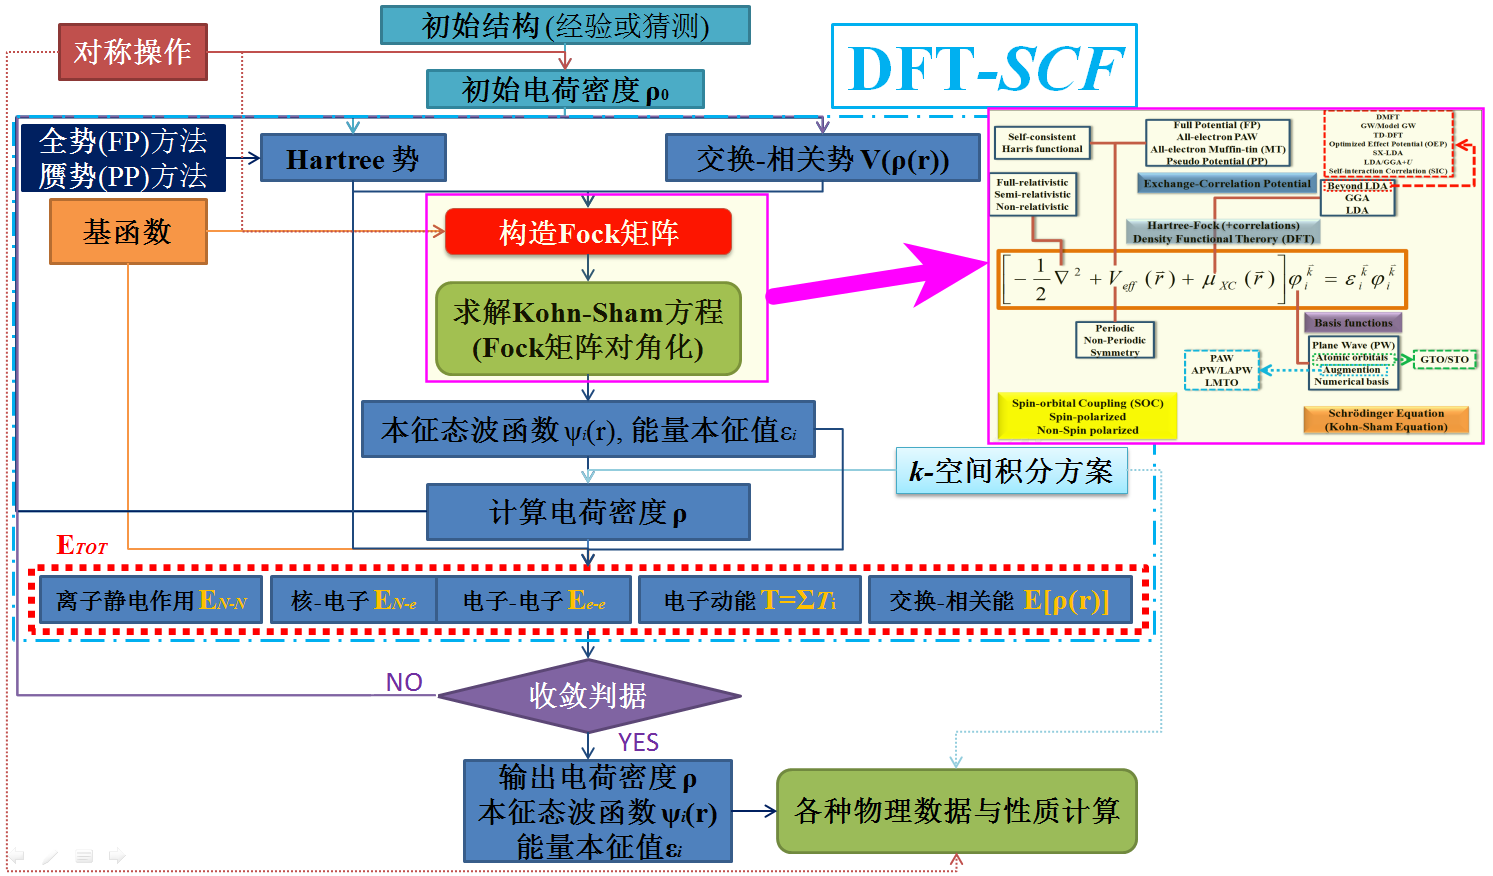
\includegraphics[height=2.80in,width=4.95in,viewport=5 3 1490 870,clip]{Figures/DFT-SCF_2.png}
%\caption{\tiny \textrm{Pseudopotential for metallic sodium, based on the empty core model and screened by the Thomas-Fermi dielectric function.}}%(与文献\cite{EPJB33-47_2003}图1对比)
\label{DFT-SCF-2}
\end{figure}
}

\frame
{
	\frametitle{\textit{ab~initio}和\textrm{first~principle}}
	\begin{itemize}
		\item \textit{ab~initio}是拉丁文词汇\textrm{(Latin~term)},其含义是\textrm{``from the beginning''},由拉丁文\textit{ab}~\textrm{(``from'')}+\textit{initio}~\textrm{(``beginning'')}合成,后者是\textit{initium}的单数夺格\footnote{\fontsize{5.5pt}{4.2pt}\selectfont{夺格\textrm{(ablative)},又称离格或从格,语法功能上表示某些词汇的状语。拉丁文\textit{initium}的意思是''开始、初始''。}}
		\item \textit{ab~initio}常用于法律和科学领域,如从头计算法(\textit{ab~initio}~\textrm{method})。法律中,\textit{ab~initio}表示"一开始即如此,而非法院宣判之后"。
		\item \textrm{first~principle}指从基本的物理学定律出发,不外加假设与经验拟合的推导与计算。
		\item 在物理学领域,\textrm{first~principle}(第一性原理)和\textit{ab~initio}(从头计算)含义上是等价的。例如利用\textrm{Schr\"odinger}方程在一些近似条件下求解电子结构,但无须依赖实验数据得到拟合参数的方法,就是第一原理或从头计算法。
	\end{itemize}
}

\frame
{
	\frametitle{\textit{ab~initio} \textrm{in inscription}}
\begin{figure}[h!]
\vspace*{-0.15in}
\centering
\includegraphics[height=2.10in,width=1.55in,viewport=5 3 1550 2180,clip]{Figures/Madonna-Ss.-Dominic-and-Thomas_Aquinas-3.jpeg}
\hspace*{15pt}
\includegraphics[height=2.10in,width=1.15in,viewport=5 3 950 1880,clip]{Figures/Madonna-Ss.-Dominic-and-Thomas_Aquinas-Inscription_2.jpeg}
%\caption{\tiny \textrm{Pseudopotential for metallic sodium, based on the empty core model and screened by the Thomas-Fermi dielectric function.}}%(与文献\cite{EPJB33-47_2003}图1对比)
\label{ABINITIO-inscription}
\end{figure}
\begin{minipage}{0.53\textwidth}
	{\fontsize{8.2pt}{4.2pt}\selectfont{ 
		\centering{MEMOR}\\
		\centering{ESTO}\\
		\centering{CONGREGATIONIS}\\
		\centering{TV\AE}\\
		\centering{QVAM}\\
		\centering{POSSEDISTI}\\
		\centering{\textcolor{red}{ABINITIO}\\}}}
\end{minipage}
\hspace*{5pt}
\begin{minipage}{0.30\textwidth}
	\textrm{\fontsize{4.2pt}{4.2pt}\selectfont{The inscription in English:}}\\
	\textrm{\fontsize{8.2pt}{4.2pt}\selectfont{\textcolor{blue}{Mind the congregation that has been yours} \textcolor{purple}{since the beginning}}}
\end{minipage}
}

%-----------------------------------------------------------------------------
\section{固体能带理论}       %Bookmark
\frame
{
%\frametitle{The Bloch theorem}
	\frametitle{\textrm{Bloch~}定理}
\begin{itemize}%[+-| alert@+>]
   \setlength{\itemsep}{8pt}
   \item 固体能带理论\upcite{Huang_Han}是固体电子理论的基础,形式上是单电子理论:
    $$\hat H |\psi_i^{\vec k}(\vec r)\rangle=\bigg[-\dfrac{\hbar^2}{2m}\nabla^2+V(\vec r)\bigg]|\psi_i^{\vec k}(\vec r)\rangle=\epsilon_i(\vec k)|\psi_i^{\vec k}(\vec r)\rangle$$
  \item \textrm{Bloch}定理:
%   \item \textrm{periodic potential:} $$V(\vec r)=V(\vec r+\vec R_n)$$
%     \textrm{Here,} $\vec R_n=n\vec R$
%   \item \textrm{Bloch theorem:}$$\psi_{\vec k}(\vec r)=\textrm{e}^{\textrm i\vec k\cdot\vec r}u_{\vec k}(\vec r)$$
%     \textrm{Here, $u_{\vec k}(\vec r)$ is a periodic function with the same periodicity as $V(\vec r)$, i.e., $u_{\vec k}(\vec r)=u_{\vec k}(\vec r+\vec R_n)$, then Bloch theorem could reads as:}
%     $$\psi_{\vec k}(\vec r+\vec R_n)=\textrm{e}^{\textrm i\vec k\cdot\vec R_n}\psi_{\vec k}(\vec r)$$
具有平移周期性的理想晶体,势能$V(\vec r)$满足$$V(\vec r)=V(\vec r+\vec R_n)$$
体系的波函数满足\textrm{Bloch}波函数形式:$$\psi_{\vec k}(\vec r)=\textrm{e}^{i\vec k\cdot\vec r}u_{\vec k}(\vec r)$$
是平面波和周期函数的乘积。$u(\vec r)$与势能有相同的周期。即$$u_{\vec k}(\vec r)=u_{\vec k}(\vec r+\vec R_n)$$
  \item 能带理论相当于分子轨道理论
%   \setlength{\itemsep}{30pt}
\item \textrm{Bloch}函数反映了波函数在周期性势场下的变化规律。
\end{itemize}
}

\frame
{
\frametitle{周期体系的波函数}
物质的电子体系,可分为芯层分子和价层电子。芯电子能量低,受周围化学环境影响很小,基本保持原子属性;价层电子相互作用较强,对化学环境较为敏感。一般地,价电子波函数在原子间区域(\textrm{Interstitial}区)的变化平缓,在临近原子核附近区域(\textrm{Muffin-tin}球内),会出现剧烈振荡(与芯层波函数正交)。
\begin{figure}[h!]
\centering
\includegraphics[height=0.8in,width=4.in,viewport=41 433 539 546,clip]{Figures/Pseudo_wave.pdf}\\
\includegraphics[height=0.8in,width=4.in,viewport=41 210 539 339,clip]{Figures/Pseudo_wave.pdf}
\caption{\tiny \textrm{The periodic Potential and the wave functions in crystal.}}%(与文献\cite{EPJB33-47_2003}图1对比)
\label{Potential-Wave}
\end{figure}
}

\frame
{
\frametitle{一维自由电子近似微扰}
\begin{figure}[h!]
\centering
%\hspace*{-10pt}
%\vspace*{-1.1in}
\includegraphics[height=1.5in,width=2.5in,viewport=5 5 700 450,clip]{Figures/Band_Gap-2.png}
%\caption{\tiny \textrm{The Band-structure from free-electron gas.}}%
\label{Band-Gap-2}
\end{figure} 
\begin{displaymath}
	\begin{aligned}
		&\hat H_0=-\dfrac{\hbar^2}{2m}\dfrac{\mathrm{d}^2}{\mathrm{d}x^2}+\={V} \longrightarrow \hat H=\hat H_0+\hat H^{\prime}=-\dfrac{\hbar^2}{2m}\dfrac{\mathrm{d}^2}{\mathrm{d}x^2}+\={V}+\underline{V(x)-\={V}}\\
		&\Psi_k^0(x)=\dfrac1{\sqrt V}\mathrm{e}^{\mathrm{i}k\cdot x} \longrightarrow \Psi_k(x)=\Psi_k^0(x)+\sum_{k^{\prime}\neq k}\dfrac{\langle k^{\prime}|\hat H^{\prime}|k\rangle}{E_k^0-E_{k^{\prime}}^0}\Psi_{k^{\prime}}^0(x)\\
		&\hat E_k^0=-\dfrac{\hbar^2k^2}{2m}+\={V} \longrightarrow E_k=%E_k^0+E^{\prime}=
		\dfrac{\hbar^2k^2}{2m}+\={V}+\sum_n{}^{\prime}\dfrac{|V_n|^2}{\frac{\hbar^2}{2m}[k^2-(k+2\pi\frac na)^2]}
	\end{aligned}
\end{displaymath}
}

\frame
{
\frametitle{一维自由电子简并微扰}
在波矢$k=\pm\frac{n\pi}{a}$位置,电子能量出现简并态,必须采用简并态微扰理论处理
\begin{figure}[h!]
\centering
%\hspace*{-10pt}
%\vspace*{-1.1in}
\includegraphics[height=1.3in,width=1.4in,viewport=0 5 420 450,clip]{Figures/Band_Gap-1.png}
%\caption{\tiny \textrm{The Band-structure from free-electron gas.}}%
\label{Band-Gap-1}
\end{figure} 
\begin{displaymath}
	E_{\textcolor{red}{\pm}}=\left\{
	\begin{aligned}
		&T_n+\={V}\textcolor{red}{+}\Delta^2T_n\bigg(\dfrac{2T_n}{|V_n|}\textcolor{red}{+}1\bigg)\\
		&T_n+\={V}\textcolor{red}{-}\Delta^2T_n\bigg(\dfrac{2T_n}{|V_n|}\textcolor{red}{-}1\bigg)
	\end{aligned}\right.
\end{displaymath}
这里$T_n=\frac{\hbar^2}{2m}\big(\frac{n\pi}a\big)^2$
}

\frame
{
\frametitle{自由电子气模型}
简并态微扰理论引起的能带裂分
\begin{figure}[h!]
\centering
%\hspace*{-10pt}
%\vspace*{-1.1in}
\includegraphics[height=2.1in,width=3.8in,viewport=10 90 570 380,clip]{Figures/Band_Gap.pdf}
\caption{\tiny \textrm{The Band-structure from free-electron gas.}}%
\label{Band-Gap-co}
\end{figure} 
}

\frame
{
\frametitle{紧束缚模型}
从分子轨道到能带
\begin{figure}[h!]
\centering
\hspace*{-0.29in}
\vspace*{-0.1in}
\subfigure[一维$\mathrm{H}$原子链]{
\label{fig:Hydrogen-1D}
\includegraphics[height=0.25in,width=1.1in,viewport=70 255 570 375,clip]{Figures/Hydrogen-1D.pdf}}
\subfigure[$\mathrm{H}_n$分子轨道]{
\label{fig:Hydrogen-2-n}
\includegraphics[height=0.8in,width=1.5in,viewport=30 140 545 480,clip]{Figures/Hydrogen-Mol-Orbital.pdf}}
\subfigure[分子波函数]{
\label{fig:Hydrogen-Psi}
\includegraphics[height=0.5in,width=1.4in,viewport=25 218 595 440,clip]{Figures/Hydrogen-Psi.pdf}}\\
\vspace*{5pt}
\subfigure[分子轨道与能带]{
\label{fig:Hydrogen-Band-1D}
\includegraphics[height=0.6in,width=1.4in,viewport=35 215 575 450,clip]{Figures/Hydrogen-Band-1D.pdf}}
\subfigure[$d$\,轨道]{
\label{fig:Hydrogen-d-Band-1D}
\includegraphics[height=1.0in,width=0.7in,viewport=40 45 330 535,clip]{Figures/Hydrogen-d-Band-1D.pdf}}
\caption{\tiny \textrm{The Band-structure from Molecular-orbital.}}%
\label{Band-Structure-local-orbit}
\end{figure} 
}

\subsection{能带、$\vec k$-空间与~\textrm{Fermi~}面}
\frame
{
\frametitle{能带、$\vec k$空间与\textrm{Fermi}面}
\vspace{30pt}
\begin{figure}[h!]
\centering
\hspace*{-0.10in}
\subfigure[\textrm{Band structure}]{
\label{Band_Gap_Fermi-1}
\includegraphics[height=1.6in,width=2.1in,viewport=0 0 480 350,clip]{Figures/Band_Brillouin_zone.png}}
\subfigure[\textrm{Brillouin Zone}]{
\label{Band_Gap_Fermi-2}
\includegraphics[height=1.28in,width=1.75in,viewport=100 120 545 470,clip]{Figures/2D_Brillouin-Zone.pdf}}
\label{Band_Gap_Fermi}
\end{figure}
}

\frame
{
	\frametitle{简单立方体系的\textrm{Brillouin}区与能带}
\vspace{10pt}
\begin{figure}[h!]
\centering
\hspace*{-0.28in}
\subfigure[\textrm{Brillouin Zone of Cubic lattice}]{
\label{Brillouin_Zone_Cubic-1}
\includegraphics[height=2.1in,width=2.0in,viewport=90 0 550 500,clip]{Figures/Brillouin-Zone_CUB.png}}
\subfigure[\textrm{Band Structure of \ch{SrSnO3}}]{
\label{Band_Gap_SrSnO3-1}
\vspace*{-1.00in}
\includegraphics[height=2.10in,width=1.75in,viewport=0 0 710 550,clip]{Figures/Band-Struct_SrSnO3.png}}
\label{Band_Gap_CUB_SrSnO3}
\end{figure}
}

\frame
{
	\frametitle{面心立方体系的\textrm{Brillouin}区与能带}
\vspace{10pt}
\begin{figure}[h!]
\centering
\hspace*{-0.30in}
\subfigure[\textrm{Brillouin Zone of FCC lattice}]{
\label{Brillouin_Zone_FCC}
\includegraphics[height=1.9in,width=1.8in,viewport=75 0 560 520,clip]{Figures/Brillouin-Zone_FCC.png}}
\subfigure[\textrm{Band structure of \ch{CdS}}]{
\label{Band_Gap_CdS}
\includegraphics[height=2.10in,width=1.95in,viewport=0 0 700 520,clip]{Figures/Band-Struct_CdS.png}}
\label{Band_Gap_FCC_CdS}
\end{figure}
}

\frame
{
	\frametitle{体心立方体系的\textrm{Brillouin}区与能带}
\vspace{10pt}
\begin{figure}[h!]
\centering
\hspace*{-0.30in}
\subfigure[\textrm{Brillouin Zone of BCC lattice}]{
\label{Brillouin_Zone_BCC}
\includegraphics[height=2.1in,width=1.9in,viewport=80 0 550 520,clip]{Figures/Brillouin-Zone_BCC.png}}
\subfigure[\textrm{Band structure of \ch{GeF4}}]{
\label{Band_Gap_GeF4}
\includegraphics[height=2.10in,width=1.95in,viewport=0 0 700 500,clip]{Figures/Band-Struct_GeF4.png}}
\label{Band_Gap_BCC_GeF4}
\end{figure}
}

\subsection{固体能带计算方法}
\frame
{
%\frametitle{The methods on band structure calculation}
\frametitle{固体能带计算方法}
%\vskip 10pt
%\textrm{The mainly difference of all these methods below: the basis sets and the construction of the potential}
\vskip 10pt
常用的计算方法
\begin{itemize}%[+-| alert@+>]
%\begin{enumerate}%[+-| alert@+>]
\setlength{\itemsep}{12pt}
%  \item \textrm{Plane wave and the pseudo-potential}
	\item	平面波方法
	\item	正交平面波\textrm{(The orthogonalized plane wave, OPW)}和赝势\textrm{(Pseudo-potential, PP)}方法\upcite{Singh,PRB41-7892_1990,JPCM6-8245_1994}
	\item	缀加平面波\textrm{(Augmented plane wave, APW)}方法
	\item	\textrm{MT}轨道\textrm{(Muffin-tin orbitals, MTO)}方法
	\item	投影子缀加波\textrm{(Projector Augmented Wave, PAW)}方法\upcite{PRB50-17953_1994,PRB59-1758_1999}
\end{itemize}
\vskip 5pt 各种方法的\textcolor{red}{主要区别}:~\textcolor{blue}{势函数的处理}与\textcolor{blue}{所选基函数类型}不同
}

\frame                               %
{
	\frametitle{\textrm{Kohn-Sham}方程}
\begin{figure}[h!]
\centering
\vspace*{-0.21in}
\hspace*{-0.1in}
\includegraphics[height=2.7in,width=4.0in,viewport=2 5 1162 880,clip]{Figures/DFT.png}
\caption{\tiny \textrm{The Analysis of Kohn-Sham equation.}}%(与文献\cite{EPJB33-47_2003}图1对比)
\label{DFT}
\end{figure}
}

\frame
{
\frametitle{电荷密度的重新分解}
%\textrm{PAW}方法提出后有很长一段时间没有能够得到广泛应用,直到\textrm{G. Kresse}等将\textrm{Bl\"ochl}的原始方案中电荷密度计算方案重新组合后,明确了\textrm{PAW}方法与\textrm{USPP}方法的内在联系。
\begin{itemize}
	\item 芯层电荷与核电荷构成离子实电荷:$n_{Zc}=n_Z+n_c$
\end{itemize}
\begin{figure}[h!]
\centering
\vspace{-10.5pt}
\includegraphics[height=1.8in,width=4.0in,viewport=0 0 380 190,clip]{Figures/Pseudo-potential_charge.png}
%\caption{\tiny \textrm{The difference of the electron-density distributing from P.~Bl\"ochl  and from G.~Kresse.}}%(与文献\cite{EPJB33-47_2003}图1对比)
\label{PAW_Pseudo-Charge}
\end{figure}
}

\section{赝势理论}       %Bookmark
%\section{Induction on DFT and solid-state physics}       %Bookmark
\subsection{平面波与赝势}       %Bookmark
\frame
{
%\frametitle{The methods on band structure calculation}
	\frametitle{由\textrm{OPW~}到赝势}
%\vskip 10pt
%\textrm{The mainly difference of all these methods below: the basis sets and the construction of the potential}
\begin{itemize}
%\setlength{\itemsep}{5pt}
	\item 完全平面波基组\\{\fontsize{7.5pt}{5.5pt}\selectfont{少数平面波就可以很好地描述波函数在原子间的行为,近核波函数则需要大量平面波展开}}%。因此完全平面波基组虽然方便,但求体系本征态对角化的矩阵非常巨大,计算变得异常耗时。
	\item 正交平面波(\textrm{Orthogonalized plane wave, OPW})方法\\{\fontsize{7.5pt}{5.5pt}\selectfont{价电子用与芯层波函数正交的平面波展开
		\begin{displaymath}
			\phi_{\textrm{OPW}}^{\vec k+\vec G}(\vec r)=\phi_{\textrm{PW}}^{\vec k+\vec G}(\vec r)-\sum_c\langle\varphi_c|\phi_{\textrm{PW}}^{\vec k+\vec G}\rangle\varphi_c(\vec r)
		\end{displaymath}}}
	{\fontsize{7.5pt}{5.5pt}\selectfont{构造赝波函数
		\begin{displaymath}
			\tilde{\phi}_v(\vec r)=\phi_v(\vec r)+\sum_c\langle\varphi_c|\tilde{\phi}_v\rangle\varphi_c(\vec r)
		\end{displaymath}
	代入\textrm{Schr\"odinger}方程
		$$\hat H|\tilde{\phi}_v\rangle-\sum_c\langle\varphi_c|\tilde{\phi}_v\rangle\hat H|\varphi_c\rangle=\varepsilon_v|\tilde{\phi}_v\rangle-\varepsilon_v\sum_c\langle\varphi_c|\tilde{\phi}_v\rangle|\varphi_c\rangle$$
		可有$$\hat H|\tilde{\phi}_v\rangle+\textcolor{blue}{V^R}|\tilde{\phi}_v\rangle=\textcolor{blue}{\varepsilon_v}|\tilde{\phi}_v\rangle$$
		这里排斥势是$$V^R(\vec r,\vec r^{\prime})=\sum_c(\varepsilon_v-\varepsilon_c)|\varphi_c(\vec r^{\prime})\rangle\langle\varphi_c(\vec r)|$$}}
\end{itemize}
}

\frame
{
	\frametitle{由\textrm{OPW~}到赝势}
	\textrm{Phillips-Kleinman}指出,赝势($V^{e\!f\!f}$)-赝波函数(可用$\phi_{PW}^{\vec k+\vec G}$展开)满足\textrm{Schr\"odinger}方程%\upcite{PR116-287_1959}
	$$\bigg(-\dfrac12\nabla^2+\textcolor{red}{V^{e\!f\!f}}\bigg)|\tilde{\phi}_v\rangle=\textcolor{blue}{\varepsilon_v}|\tilde{\phi}_v\rangle$$
	其中$\textcolor{red}{V^{e\!f\!f}}=V(\vec r)+\textcolor{blue}{V^R}$
	\begin{itemize}
		\item 赝势-赝波函数的本征值$\varepsilon_v$与真实体系的价电子能量本征值等价
		\item 赝势$\textcolor{red}{V^{e\!f\!f}}$比$V(\vec r)$平滑得多,并且$\textcolor{blue}{V^R}$是非局域的排斥势
			\begin{displaymath}
				\begin{aligned}
					\textcolor{blue}{V^R}f(\vec r)=&\sum_c(\varepsilon_v-\varepsilon_c)\varphi_c(\vec r)\int\varphi_c^{\ast}(\vec r^{\prime})f(\vec r^{\prime})\mathrm{d}\vec r^{\prime} \\
					=&\int V^R(\vec r,\vec r^{\prime})f(\vec r^{\prime})\mathrm{d}\vec r^{\prime}
				\end{aligned}
			\end{displaymath}
%			这里$$V^R(\vec r,\vec r^{\prime})=\sum_c(\varepsilon_v-\varepsilon_c)|\varphi_c(\vec r^{\prime})\rangle\langle\varphi_c(\vec r)|$$
	\end{itemize}
}

\frame
{
\frametitle{赝势的评估}
赝势(\textrm{Pseudo Potential, PP})方法是在正交平面波的基础上发展起来的,构造出平缓的势函数代替核的强吸引作用和芯层电子的排斥作用,用平缓的函数取代波函数近核时的震荡。
\begin{itemize}
\setlength{\itemsep}{5pt}
	\item 赝势-平面波方法,只需要少量平面波可展开赝波函数,大大提升了计算效率;但是赝波函数不能很好地反映与电子近核行为有关的性质。
	\item 赝势的构造并不唯一,考核构造赝势的两大指标:~\\“柔软程度”\textrm{(Soft)}与“可移植性”\textrm{(transferability)}
\end{itemize}
\begin{figure}[h!]
\centering
\vspace*{-0.10in}
\includegraphics[height=1.35in,width=1.40in,viewport=154 100 562 508,clip]{Figures/Pseudo.pdf}
\includegraphics[height=1.35in,width=2.55in,viewport=1 1 980 500,clip]{Figures/Pseudo-2.png}
\caption{\tiny \textrm{The Pseudo wave function and Pseudo potential.}}%(与文献\cite{EPJB33-47_2003}图1对比)
\label{Pseudo_Potential-Wave}
\end{figure}
}

\frame
{
	\frametitle{传统赝势的构造}
	直接由实验数据来确定(模型)赝势,常用的实验数据包括离子对电子的散射角度、离子的光谱实验数据等
		\begin{itemize}
			\item 构造离子赝势:~可移植性好
			\item 构造总赝势(包括全部价电子相互作用):~常用于能带描述
		\end{itemize}
%	\begin{itemize}
%		\item 在指定能量范围内,离子对电子散射的散射角
%		\item 离子的光谱实验数据
%	\end{itemize}
\begin{figure}[h!]
\centering
\vspace*{-0.10in}
\includegraphics[height=1.60in,width=2.57in,viewport=0 0 980 600,clip]{Figures/Pseudo-model-empty_core.png}
\caption{\tiny \textrm{Pseudopotential for metallic sodium, based on the empty core model and screened by the Thomas-Fermi dielectric function.}}%(与文献\cite{EPJB33-47_2003}图1对比)
\label{Pseudo_model-empty_core}
\end{figure}
}

\frame
{
	\frametitle{传统赝势的构造}
\begin{figure}[h!]
\centering
\vspace*{-0.10in}
\includegraphics[height=1.30in,width=4.17in,viewport=0 0 1150 350,clip]{Figures/Pseudo-model.png}
\caption{\tiny \textrm{Left:``Empty core'' model potential of Ashcroft in which the potential is zero inside radius $R_c(l)$ which is different for each $l$. Right: Square well model potential with value $A_l$ inside a cut-off radius $R_c$, proposed by Abarenkov and Heine and fit to atomic data by Animalu and Heine. The fact that the potential are weak, zero, or even positive inside cut-off radius $R_c$ is an illustration of the ``cancellation theorem''.}}%(与文献\cite{EPJB33-47_2003}图1对比)
\label{Pseudo-model}
\end{figure}
}

\subsection{模守恒赝势}
\frame
{
	\frametitle{第一原理赝势}
		由第一原理求解出全电子波函数(径向部分)$P_{n,l}(r)$
			\begin{displaymath}
				\bigg[-\dfrac12\dfrac{\mathrm{d}^2}{\mathrm{d}r^2}+\dfrac{l(l+1)}{2r^2}+V(\rho,r)\bigg]P_{n,l}(r)=\varepsilon_{n,l}P_{n,l}(r)
			\end{displaymath}
			这里$V(\rho,r)$是自洽单电子势
			$$V(\rho,r)=-\frac{Z}r+V_{\mathrm H}(\rho,r)+V_{XC}^{\mathrm{LDA}}(\rho(r))$$
			$V_{\mathrm H}(\rho,r)$是\textrm{Hartree}势,$V_{XC}^{\mathrm{LDA}}(\rho(r))$是交换-相关势

			由此构造赝波函数$P_l^{\mathrm{PP}}(r)$,满足
			$$P_l^{\mathrm{PP}}(r)=P_l^{\mathrm{AE}}(r),\quad r>r_{l}^c$$
			进而构造赝势$V_{\mathrm{src},l}^{\mathrm{PP}}(r)$
			$$V_{\mathrm{src},l}^{\mathrm{PP}}(r)=\varepsilon_l-\dfrac{l(l+2)}{2r^2}+\dfrac{1}{2P_l^{\mathrm{PP}}(r)}\dfrac{\mathrm{d}^2}{\mathrm{d}r^2}P_l^{\mathrm{PP}}(r),\quad r<r_{l}^c$$
}

\frame
{
	\frametitle{模守恒\textrm{(Norm-conserving)}条件}
%	构造赝势确定参数的边界(构造条件)
	\begin{enumerate}
		\item 价电子赝波函数的能量本征值与对应全电子波函数能量本征值相等:~$\varepsilon_l^{\mathrm{PP}}=\varepsilon_l^{\mathrm{AE}}$
		\item 价电子赝波函数与真实电子波函数的径向部分在截断半径$r_{c,l}$外相同:~$\psi_l^{\mathrm{PP}}(r)=\psi_l^{\mathrm{AE}}(r),\quad r>r_{l}^c$
		\item 价电子赝波函数与真实电子波函数的对数导数在截断半径$r_{c,l}$处相等:~$D_l^{\mathrm{PP}}(r)=D_l^{\mathrm{AE}}(r),\quad r\geqslant r_{l}^c$\\
		这里$D_l(\varepsilon,r)=r\frac{\psi_l^{\prime}(\varepsilon,r)}{\psi_l(\varepsilon,r)}=r\dfrac{\mathrm{d}}{\mathrm{d}r}\ln\psi_l(\varepsilon,r)$
		\item 价电子赝波函数与真实电子波函数在截断半径$r_{l}^c$内的积分电荷相等(\textcolor{red}{模守恒条件})
			$$Q_l=\int_0^{r_{l}^c}\mathrm{d}rr^2|\psi_l^{\mathrm{PP}}(r)|^2=\int_0^{r_{l}^c}\mathrm{d}rr^2|\psi_l^{\mathrm{AE}}(r)|^2$$
		\item 价电子赝波函数与真实电子波函数的对数导数一阶能量导数$\mathrm{d}D_l(\varepsilon,r)/\mathrm{d}\varepsilon$在截断半径$r_{l}^c$处及以外相等
	\end{enumerate}
}

\frame
{
	\frametitle{模守恒\textrm{(Norm-conserving)}条件}
\begin{figure}[h!]
\centering
\vspace*{-0.10in}
\includegraphics[height=1.30in,width=4.17in,viewport=0 0 1150 350,clip]{Figures/Pseudo-OPW_NCPP.png}
\caption{\tiny \textrm{Schematic example of a valence function that has the character of a $3s$ orbital near the nucleus and two examples of smooth functions (dashed lines) that equal the full wave-function outside the core region. Left: the smooth part of the valence function defined by OPW-like equation; Right: a smooth pseudo-function that satisfies the norm-conservation condition.}}%(与文献\cite{EPJB33-47_2003}图1对比)
\label{Pseudo-OPW_NCPP}
\end{figure}
}

\frame
{
	\frametitle{赝势去屏蔽}
	第一原理赝势建立了赝波函数与对应赝势的一一对应关系,但该赝势包含了电子屏蔽(原子、离子环境)信息,去屏蔽后的赝势对环境依赖更低,“可移植性”更好
	$$V_{\mathrm{ion},l}^{\mathrm{PP}}(r)=V_{\mathrm{src},l}^{\mathrm{PP}}(r)-V_{\mathrm{H},l}^{\mathrm{PP}}(r)-V_{XC,l}^{\mathrm{PP}}(r)$$
	去屏蔽过程中,特别需要注意$V_{XC,l}^{\mathrm{PP}}(r)$的处理
	$$V_{XC,l}^{\mathrm{PP}}(r)=V_{XC}^{\mathrm{PP}}([n_l^{\mathrm{PP}}],r)+\big[V_{XC}^{\mathrm{PP}}([n_l^{\mathrm{PP}}+n^{core}],r)-V_{XC}^{\mathrm{PP}}([n_l^{\mathrm{PP}}],r)\big]$$
}

\frame
{
	\frametitle{非局域赝势}
	当前第一原理赝势径向部分是局域的,但与$l$有关,因此是半局域的(\textrm{semi-local})
	\begin{displaymath}
		\hat{V}^{\mathrm{SL}}=\sum_{lm}|Y_{lm}\rangle V_l(r)\langle Y_{lm}|
	\end{displaymath}
	将赝势的径向部分分解为局域部分($l$无关)和非局域部分($l$相关)
	\begin{displaymath}
		V_{\mathrm{ion},l}^{\mathrm{PP}}(r)=V_{\mathrm{local}}^{\mathrm{PP}}(r)+\delta V_l^{\mathrm{PP}}(r)
	\end{displaymath}
	第一原理赝势可以表示为
	\begin{displaymath}
		\hat{V}^{\mathrm{SL}}=V_{\mathrm{local}}^{\mathrm{PP}}(r)+\sum_{lm}|Y_{lm}\rangle\delta V_l(r)\langle Y_{lm}|
	\end{displaymath}
	赝势的非局域部分可以表示为
	\begin{displaymath}
		\delta V(\vec r,\vec r^{\prime})=\sum_{lm}|Y_{lm}\rangle\delta V_l(r)\langle Y_{lm}|
	\end{displaymath}
}

\frame
{
	\frametitle{模守恒赝势构造流程}
\begin{figure}[h!]
\centering
%\vspace*{-0.10in}
\includegraphics[height=2.70in,width=3.77in,viewport=70 40 900 610,clip]{Figures/Pseudo-NC.jpg}
%\caption{\tiny \textrm{Pseudopotential for metallic sodium, based on the empty core model and screened by the Thomas-Fermi dielectric function.}}%(与文献\cite{EPJB33-47_2003}图1对比)
\label{Pseudo-NC}
\end{figure}
}

\subsection{可分离赝势与\rm{Ghost~band}}
\frame
{
	\frametitle{非局域赝势的变量分离}
	\textrm{Kleinman-Bylander}提出了非局域赝势的变量分离的近似方案\footnote{即$\delta V(\vec r,\vec r^{\prime})$可以写成$\delta V(\vec r,\vec r^{\prime})=\sum_{i}f_i(\vec r)g_i(\vec r^{\prime})$的形式}:~\\
%	引入分离算符$\delta V^{\mathrm{NL}}$满足
	{\fontsize{7.2pt}{5.2pt}\selectfont{如果选择适当的局域函数$V_{\mathrm{local}}^{\mathrm{PP}}(r)$,赝势将可分解为局域部分与非局域部分之和:
	$$\hat V_{\mathrm{NL}}^{\mathrm{PP}}(r)=V_{\mathrm{local}}^{\mathrm{PP}}(r)+\sum_{lm}\dfrac{|\psi_{lm}^{\mathrm{PP}}\delta V_l\rangle\langle\delta V_l\psi_{lm}^{\mathrm{PP}}|}{\langle\psi_{lm}^{\mathrm{PP}}|\delta V_l|\psi_{lm}^{\mathrm{PP}}\rangle}$$ 
	\textcolor{magenta}{$\langle\delta V_l(r)\psi_{lm}^{\mathrm{PP}}|$是投影子},这种分解称为\textrm{factored pseudo-potential},方便数值计算
\vskip 10pt
	更一般地,如果允许赝势局域部分$V_{\mathrm{local}}^{\mathrm{PP}}(r)$为任意函数,则可定义辅助函数
	$$\chi_{lm}^{\mathrm{PP}}(\vec r)=\bigg\{\varepsilon_l-\bigg[-\dfrac12\nabla^2+V_{\mathrm{local}}^{\mathrm{PP}}(\vec r)\bigg]\bigg\}\psi_{lm}^{\mathrm{PP}}(\vec r)$$
	于是赝势的非局域部分可表示为
	$$\delta V_{\mathrm{NL}}=\sum_{lm}\dfrac{|\chi_{lm}^{\mathrm{PP}}\rangle\langle\chi_{lm}^{\mathrm{PP}}|}{\langle\chi_{lm}^{\mathrm{PP}}|\psi_{lm}^{\mathrm{PP}}\rangle}$$
但是$V_{\mathrm{local}}^{\mathrm{PP}}(r)$选择的随意性,将增加计算结果出现\textrm{Ghost~band}的风险
}}
}

\frame
{
	\frametitle{\textrm{Ghost~band}的表现}
	\fontsize{9.2pt}{4.2pt}\selectfont{只有价电子的赝波函数与芯电子波函数完全正交,能带计算中才能确保芯层与价层电子的完全分离。但实际计算时,该正交条件很难严格保证,因此一旦赝波函数严重偏离正交条件,计算的能带中会在本不存在能带的区域出现电子结构分布(称为\textrm{Ghost~band}),这部分电子结构源自构造赝波函数的能量参数$\varepsilon_l$与芯层电子能量差别太大,无法保持与芯层电荷严格正交引起的}
\begin{figure}[h!]
\centering
\vspace*{-0.10in}
\includegraphics[height=1.50in,width=1.98in,viewport=0 0 450 320,clip]{Figures/Ghostband-Vanadium-1.png}
\includegraphics[height=1.50in,width=1.98in,viewport=0 0 450 320,clip]{Figures/Ghostband-Vanadium-4.png}
\caption{\fontsize{7.2pt}{4.2pt}\selectfont{\textrm{The band structure of bcc Vanadium. %In the calculation, all electrons up to the 3p states were treated as core electrons, all other electrons as valence electrons. 
\\Left:~Between 10 and 15 eV above the Fermi energy a strange band with nearly no dispersion can be observed. The vanishing dispersion of the band is a typical property of ghost bands.}}}%(与文献\cite{EPJB33-47_2003}图1对比)
\label{Ghost-band}
\end{figure}
}

\frame
{
	\frametitle{\textrm{Ghost~band}的根源}
	可分离赝势方法中
	\begin{displaymath}
		\hat{\mathbf{H}}=-\dfrac12\nabla^2+V_{\mathrm{local}}(r)+\delta\hat{V}_{\mathrm{NL}}
	\end{displaymath}
	赝波函数$\psi_{lm}^{\mathrm{PP}}(r)$是方程
	\begin{displaymath}
		\hat{\mathbf{H}}\psi_{lm}^{\mathrm{PP}}(r)=\varepsilon_l\psi_{lm}^{\mathrm{PP}}(r)
	\end{displaymath}
	的解。
\vskip 15pt
	因为$V_{\mathrm{local}}(r)$可随意选择,因此赝波函数$\psi_{lm}^{\mathrm{PP}}(r)$和能量$\varepsilon_l$不再要求与束缚态波函数相对应,将导致\textrm{Ghost~band}的出现
}

\frame
{
	\frametitle{\textrm{Ghost~band}根源的数学说明$^{\ast}$}
	{\fontsize{7.2pt}{5.2pt}\selectfont{对于半局域势,求解能量$\varepsilon$对应的径向波函数$u_l(r,\varepsilon)$的方程\textcolor{blue}{是一个常微分方程}
		\begin{displaymath}
			-\dfrac12\dfrac{\mathrm{d}^2u_l}{\mathrm{d}r^2}+\overline{V}_l^{\mathrm{loc}}(r)u_l(r,\varepsilon)+\Delta V_l^{\mathrm{SL}}(r)u_l(r,\varepsilon)-\varepsilon u_l(r,\varepsilon)=0
		\end{displaymath}
		而对于可分离赝势(如\textrm{KB}势),方程则为\textcolor{blue}{积分-微分方程}
		\begin{displaymath}
			-\dfrac12\dfrac{\mathrm{d}^2u_l}{\mathrm{d}r^2}+\overline{V}_l^{\mathrm{loc}}(r)u_l(r,\varepsilon)+\int\Delta V_l(r,r^{\prime})u_l(r^{\prime},\varepsilon)\mathrm{d}r^{\prime}-\varepsilon u_l(r,\varepsilon)=0
		\end{displaymath}
		将可分离赝势代入可有
		\begin{displaymath}
			-\dfrac12\dfrac{\mathrm{d}^2u_l}{\mathrm{d}r^2}+\overline{V}_l^{\mathrm{loc}}(r)u_l(r,\varepsilon)+f_l(r)\int g_l(r^{\prime})u_l(r^{\prime},\varepsilon)\mathrm{d}r^{\prime}-\varepsilon u_l(r,\varepsilon)=0
		\end{displaymath}
		\begin{itemize}
			\item \textcolor{blue}{常微分方程解的结构服从\textrm{Wronskian}定理的推论:~本征态能量$\varepsilon_0,\varepsilon_1,\cdots,\varepsilon_n$按升序排列时,对应的本征态波函数(径向)的节点数依次递增}
			\item \textcolor{red}{积分-微分方程解的结构不要求满足该结论:~波函数的节点数与能量本征态不再有对应的升序关系}
		\end{itemize}
		由于积分项的存在,传统的常微分方程求解算法(如\textrm{Runger-Kutta}法等)无法直接用于该积分-微分方程,必须另图别策
	}}
}

\frame
{
	\frametitle{\textrm{Ghost~band}根源的数学说明$^{\ast}$}
		{\fontsize{7.2pt}{5.2pt}\selectfont{
		基本思想:~类似积分方程求解的\textrm{Fredholm}方法
		\begin{itemize}
			\item 先将微分方程中的\textcolor{magenta}{积分项近似为常数因子},\textcolor{blue}{求解非齐次常微分方程}
			\item 对含有波函数的积分,应用闭路积分公式\textrm{(closure formula)}计算
		\end{itemize}}}
		{\fontsize{5.2pt}{5.2pt}\selectfont{具体求解流程
		\begin{enumerate}
			\item 采用通用方法分别求解\\\textcolor{blue}{齐次微分方程}
				\begin{displaymath}
					-\dfrac12\dfrac{\mathrm{d}^2W_l}{\mathrm{d}r^2}+\overline{V}_l^{\mathrm{loc}}(r)W_l(r,\varepsilon)-\varepsilon W_l(r,\varepsilon)=0
				\end{displaymath}
				的通解和\\\textcolor{magenta}{不含积分项的}\textcolor{blue}{非齐次微分方程}
				\begin{displaymath}
					-\dfrac12\dfrac{\mathrm{d}^2X_l}{\mathrm{d}r^2}+\overline{V}_l^{\mathrm{loc}}(r)X_l(r,\varepsilon)-\varepsilon X_l(r,\varepsilon)=f_l(r)
				\end{displaymath}
				的一个特解
			\item 构造积分
				\begin{displaymath}
					\begin{aligned}
					\tilde {W}(\varepsilon)=&\int g_l(r)W(r,\varepsilon)\mathrm{d}r\\
					\tilde {X}(\varepsilon)=&1+\int g_l(r)X(r,\varepsilon)\mathrm{d}r
					\end{aligned}
				\end{displaymath}
			\item 由此得到积分-微分方程的解
				\begin{displaymath}
					u(r,\varepsilon)=K[W(r,\varepsilon)\tilde{X}(\varepsilon)-X(r,\varepsilon)\tilde{W}(\varepsilon)]
				\end{displaymath}
		这里$K$是归一化因子	
		\end{enumerate}
	}}
}

\frame
{
	\frametitle{\textrm{Ghost~band}的克服}
	{\fontsize{7.2pt}{5.2pt}\selectfont{根据微分方程理论
	\begin{displaymath}
		\hat{\mathbf{H}}\psi_{lm}^{\mathrm{PP}}(r)=\varepsilon_l\psi_{lm}^{\mathrm{PP}}(r)
	\end{displaymath}
	的解$\psi_{lm}^{\mathrm{PP}}(r)$可表示为(只考虑径向部分)
	\begin{displaymath}
		\psi_{l}^{\mathrm{PP}}(r)=u_l^0(r)+\sum_ic_iu_l^i(r)
	\end{displaymath}
这里$u_l^0(r)$和$u_l^i(r)$分别是
齐次微分方程
	\begin{displaymath}
		\bigg(-\dfrac12\nabla^2+V_{\mathrm{local}}-\varepsilon_l^0\bigg)u_{l}^0(r)=0
	\end{displaymath}
和非齐次微分方程
	\begin{displaymath}
		\bigg(-\dfrac12\nabla^2+V_{\mathrm{local}}-\varepsilon_l^j\bigg)u_{l}^j(r)=\chi_{l}^j(r)
	\end{displaymath}
的解

引入多个能量参数$\varepsilon_l^i$,通过优化控制参数$c_i$,可以得到理想的局域势函数$V_{\mathrm{local}}(r)$
}}
}

\frame
{
	\frametitle{广义模守恒条件}
	为提高模守恒赝势的可移植性\footnote{\tiny{换言之,提升赝波函数能适应的能量变分空间}},\textrm{Vanderbilt}和\textrm{Bl\"ochl}分别建议:\\
	在构造可分离赝势时,\textcolor{blue}{引入额外的参考能量$\varepsilon_l$,并要求对每个角动量量子数$l$,所有能量参数$\varepsilon_l$构造的赝波函数$\phi_i^{\mathrm{ps}}$及其辅助函数$\chi_i$都满足
	\begin{displaymath}
		|\chi_i\rangle=-(\mathbf{T}+V_{\mathrm{loc}}-\varepsilon)|\phi_i^{\mathrm{ps}}\rangle
	\end{displaymath}}
	{\fontsize{7.2pt}{5.2pt}\selectfont{这里$i$表示量子数$l$,$m$和能量参数$\varepsilon$,即$i=(lm,\varepsilon)$}}
	\vskip 5pt
	由此出发,可构造出一组与赝波函数$\phi_i^{\mathrm{ps}}$垂直的函数$\beta_i$:~
{\fontsize{7.2pt}{5.2pt}\selectfont{
	\begin{itemize}
		\item 构造矩阵$\mathbf{B}$,其矩阵元$B_{ij}$满足
			\begin{displaymath}
				B_{ij}= \langle\phi_j^{\mathrm{ps}}|\chi_i\rangle
			\end{displaymath}
		\item 由矩阵$\mathbf{B}$和$\chi$得到函数$\beta_i$
			\begin{displaymath}
				|\beta_i\rangle=\sum_j(\mathbf{B}^{-1})_{ij}|\chi_j\rangle
			\end{displaymath}
		\item 由此得到的$\beta$与赝波函数$\phi_i^{\mathrm{ps}}$满足正交条件
	\begin{displaymath}
		\langle\beta_i|\phi_j^{\mathrm{ps}}\rangle=\delta_{ij}
	\end{displaymath}
	\end{itemize}}}
}

\frame
{
	\frametitle{广义模守恒条件}
	因此可分离赝势的非局域部分表示为
	\textcolor{blue}{\begin{displaymath}
		V_{\mathrm{NL}}=\sum_i|\chi_i\rangle\langle\beta_i|=\sum_{ij}B_{ij}|\beta_j\rangle\langle\beta_i|
	\end{displaymath}}
	{\fontsize{7.2pt}{5.2pt}\selectfont{不难看出,如果赝波函数满足广义模守恒条件
	\begin{displaymath}
		Q_{ij}=\langle\phi_j^{\mathrm{AE}}|\phi_i^{\mathrm{AE}}\rangle-\langle\phi_j^{\mathrm{PS}}|\phi_i^{\mathrm{PS}}\rangle = 0
	\end{displaymath}
	亦即
	\begin{displaymath}
		Q_{l\varepsilon,l\varepsilon^{\prime}}=\int_0^{R_c}\bigg(\phi_{l\varepsilon}^{\mathrm{AE}}(r)\phi_{l\epsilon^{\prime}}^{\mathrm{AE}}(r)-\phi_{l\varepsilon}^{\mathrm{PS}}(r)\phi_{l\varepsilon^{\prime}}^{\mathrm{PS}}(r)\bigg)\mathrm{d}r=0
	\end{displaymath}
	将大大提高赝势的可移植性。
	\vskip 5pt
	但实际上,广义模守恒条件看似简单,当能量参数$\varepsilon\neq\varepsilon^{\prime}$,要满足这个条件
	$$Q_{l\varepsilon,l\varepsilon^{\prime}}=0$$
	并非易事;~而一旦模守恒条件被破坏,矩阵$\mathbf{B}$(相应地,赝势的非局域部分$V_{\mathrm{NL}}$)就是非\textrm{Hermitian}}}
}

\subsection{超软赝势}
\frame
{
\frametitle{超软赝势}
\begin{itemize}
\setlength{\itemsep}{5pt}
	\item 赝势构造的模守恒条件
%		\begin{displaymath}
%			\int_0^{r_c}\mathrm{d}\vec r\varphi^{\ast PS}(\vec r)\varphi^{PS}(\vec r)=\int_0^{r_c}\mathrm{d}\vec r\varphi^{\ast}(\vec r)\varphi(\vec r)
%		\end{displaymath}
	很好地解决了赝势可移植性问题,但对$1s$、$2p$、$3d$等轨道,模守恒方案构造的赝势过于“硬”,所需平面波基组依然非常大
	\item 超软\textrm{(Ultra-soft)}赝势,解除模守恒条件,实现对第一、第二周期元素的高效计算
\end{itemize}
\begin{figure}[h!]
\vspace*{-0.10in}
\centering
\includegraphics[height=1.35in,width=1.40in,viewport=30 55 415 500,clip]{Figures/Norm-US-wave.pdf}
\caption{\tiny \textrm{Oxygen 2} \textit{p} \textrm{radical wave function (solid), NC-pseudo-wave (dotted) and US-pseudo-wave (dashed).}}%(与文献\cite{EPJB33-47_2003}图1对比)
\label{Norm-US-wave}
\end{figure}
}

\frame
{
\frametitle{补偿电荷与多极矩}
根据电动力学定理:\\\textcolor{blue}{如果球\textrm{S}内的电荷密度分布$\rho(\vec r)$,在球外某点$\vec r$产生的势是由电荷密度的多极矩确定}:
\begin{figure}[h!]
\vspace*{-15pt}
\centering
\includegraphics[height=1.25in,width=1.32in,viewport=1 22 507 575,clip]{Figures/potential_multipole.jpg}
%\caption{\tiny \textrm{From Muffin-tin Potential to Full Potential}}%(与文献\cite{EPJB33-47_2003}图1对比)
\label{Potential-multipole}
\end{figure}
\begin{displaymath}
	V(\vec r)=\sum_{l=0}^{\infty}\sum_{m=-l}^{l}\dfrac{4\pi}{2l+1}q_{lm}\dfrac{Y_{lm}(\hat{\vec r})}{r^{l+1}}
\end{displaymath}
其中多极矩$q_{lm}$由下式计算
\begin{displaymath}
	q_{lm}=\int_SY_{lm}^{\ast}(\hat{\vec r})r^l\rho(\vec r)\mathrm{d}^3r
\end{displaymath}
}

\frame
{
\frametitle{超软赝势的构造}
\textrm{Vanderbilt}建议构造赝波函数时放弃模守恒约束条件,只要求价电子赝波函数与真实电子波函数的径向部分在截断半径$r_{l}^c$外相同,由此得到的赝势显然非\textrm{Hermitian},但是通过构造\\\textcolor{blue}{\textrm{Hermitian}重叠算符}
\begin{displaymath}
	\mathbf{S}=\mathbf{1}+\sum_{i,j}Q_{ij}|\beta_j\rangle\langle\beta_i|
\end{displaymath}
以及\textcolor{blue}{\textrm{Hermitian}赝势算符}
\begin{displaymath}
	\tilde V^{\mathrm{NL}}=\sum_{i,j}\mathbf{D}_{i,j}|\beta_j\rangle\langle\beta_i|
\end{displaymath}
这里\textcolor{blue}{
\begin{displaymath}
	\mathbf{D}_{ij}=B_{ij}+\varepsilon_iQ_{ij}
\end{displaymath}}
模守恒约束下的标准本征值方程将变成广义本征值方程
\begin{displaymath}
	(T+V_{\mathrm{loc}}+\tilde V^{\mathrm{NL}}-\varepsilon\mathbf{S})|\phi\rangle=0
\end{displaymath}
}

\frame
{
\frametitle{超软赝势的特点}
\textrm{Vanderbilt}的超软赝势构造方案最大的优点是
\begin{itemize}
	\item \textcolor{purple}{解除模守恒约束}:~有助于增加赝波函数的截断半径,系统提高赝势的柔软程度
	\item \textcolor{purple}{引入多个参考能量$\varepsilon_l$}:~使得模守恒条件下只在特定参考能量$\varepsilon$处成立的对数导数连续条件,扩展到参考能量$\varepsilon_l$区间范围内,这大大提高了赝势的适用范围(可移植性)
\end{itemize}

相应的,超软赝势计算中,电子密度表达形式为
\begin{displaymath}
	n(r)=\sum_nf_n|\phi_n(r)|^2+\sum_{n,ij}f_n\langle\phi_n|\beta_j\rangle\langle\beta_i|\phi_n\rangle Q_{ij}(r)
\end{displaymath}
这里补偿电荷$Q_{ij}(r)$定义为
\begin{displaymath}
	Q_{ij}(r)=\phi_i^{\mathrm{AE}}(r)\phi_j^{\mathrm{AE}}(r)^{\ast}-\phi_i^{\mathrm{US}}(r)\phi_j^{\mathrm{US}}(r)^{\ast}
\end{displaymath}
}

\subsection{基态总能量表达式}
\frame
{
	\frametitle{晶体总能量的一般表示\footnote{本部分参阅文献\cite{JPC-SSP12-4409_1979,Xie-Lu,Elect_Stru}}}
采用赝势方法计算的晶体总能量$E_T$由晶格中的电子能量$E_{e-e}$与离子实排斥能$E_{N-N}$之和:
	\begin{displaymath}
		E_T=E_{e-e}+E_{N-N}=\textcolor{blue}{T[\rho]+E_{ext}+E_{\mathrm{Coul}}}+E_{\mathrm{XC}}+E_{N-N}
	\end{displaymath}
根据\textrm{Kohn-Sham}方程,其中动能泛函用单电子能量表示为
\begin{displaymath}
	T[{\rho}]=\sum_in_i\langle\psi_i|\varepsilon_i-V_{\mathrm{KS}}|\psi_i\rangle
\end{displaymath}
$n_i$是$\psi_i$上的电子占据数,$\varepsilon_i$是其能量本征值,因此有
\begin{displaymath}
	\hspace*{-12.0pt}	E_T=\textcolor{blue}{\sum_in_i\varepsilon_i-\dfrac12\iint\mathrm{d}\vec r\mathrm{d}\vec r\dfrac{\rho(\vec r)\rho(\vec r^{\prime})}{|\vec r-\vec r^{\prime}|}}+\int\mathrm{d}\vec r\rho(\vec r)[\epsilon_{\mathrm{XC}}(\vec r)-V_{\mathrm{XC}}(\vec r)]+E_{N-N}
\end{displaymath}
}

\frame
{
	\frametitle{晶体总能量倒空间的表示}
周期体系的总能量表达式在动量空间($\vec K$空间)计算更方便
\begin{displaymath}
	\hspace*{-15.0pt}	E_T=\textcolor{red}{\sum_in_i\varepsilon_i}-\dfrac{\Omega}2\sum_{\textcolor{red}{\vec k\neq 0}}\rho^{\ast}(\vec k)V_{\mathrm{Coul}}(\vec k)+\Omega\sum_{\vec k}\rho^{\ast}(\vec k)[\epsilon_{\mathrm{XC}}(\vec k)-V_{\mathrm{XC}}(\vec k)]+\textcolor{red}{E_{N-N}}
\end{displaymath}
其中$V_{\mathrm{Coul}}(\vec k)$、$\epsilon_{\mathrm{XC}}(\vec k)$与$\rho^{\ast}(\vec k)$分别是\textrm{Coulomb}相互作用、单个电子的交换-相关能、交换-相关势和电子密度的\textrm{Fourier}分量。

由\textrm{Poisson}方程
\begin{displaymath}
	\nabla^2V_{\mathrm{Coul}}(\vec r)=-4\pi\rho(\vec r)
\end{displaymath}
的\textrm{Fourier}展开有
\begin{displaymath}
	V_{\mathrm{Coul}}(\vec k)=\dfrac{4\pi\rho^{\ast}(\vec k)}{|\vec k|^2}
\end{displaymath}
交换-相关势和交换-相关能的计算一般先在实空间计算$\epsilon_{\mathrm{XC}}(\vec r)$和$V_{\mathrm{XC}}(\vec r)$后,再通过\textrm{Fourier}变换到动量空间,得到$\epsilon_{\mathrm{XC}}(\vec k)$和$V_{\mathrm{XC}}(\vec k)$
}

\frame
{
	\frametitle{晶体离子相互作用的计算}
	离子间\textrm{Coulomb}相互作用能之和
	\begin{displaymath}
		E_{N-N}=\dfrac12\sum_{\vec R,s}\sideset{}{^{\prime}}\sum_{\vec R^{\prime},\vec s^{\prime}}\dfrac{Z_sZ_{s^{\prime}}}{|\vec R+\vec r_s-\vec R^{\prime}-\vec r_s^{\prime}|}
	\end{displaymath}
	这里$Z_s$是离子实的电荷数,$\vec R$表示晶格点的位矢,$\vec r_s$代表元胞内原子的相对位矢。

	\textcolor{red}{\textbf{注意}}:~$E_{N-N}$求和有无穷多项,\textcolor{red}{是发散的};~$V_{\mathrm{Coul}}(\vec k=0)$\textcolor{red}{是发散的}
	
	$V_{ext}$在不存在其他外场时,一般只考虑离子-电子的\textrm{Coulomb}相互作用,
	\begin{displaymath}
%		\begin{aligned}
			V_{ext}(\vec r)=\sum_{\vec R,s}\dfrac{-Z_s}{|\vec r-\vec R-\vec r_s|}\equiv\sum_{\vec R,s}v_{ext}^s(\vec r-\vec R-\vec r_s)
%		\end{aligned}
	\end{displaymath}
	$V_{ext}$的\textrm{Fourier}分量在$\vec k=0$\textcolor{red}{也是发散的}
}

\frame
{
	\frametitle{晶体总能量计算的奇点排除}
这三项单独都是发散的,但因为整个体系出于电中性,所以这些发散项相互抵消,是一个常数。因此求解\textrm{Kohn-Sham}方程时,先将$V_{\mathrm{Coul}}(\vec k=0)$和$V_{ext}(\vec k=0)$同时置为零,这相当于\textcolor{red}{将势能作一平移,或者说重新定义势能零点,而在总能量计算中补偿这一平移。}
\begin{figure}[h!]
	\begin{center}
		\includegraphics[height=0.65in,width=1.50in,viewport=0 0 1250 565,clip]{Figures/Ewald_method-3.png}
	\end{center}
	\caption{\fontsize{5.5pt}{2.2pt}\selectfont{\textrm{A lattice of point charge in a uniform compensating background as considered in the Ewald calculation.}}}
	\label{fig:Ewald-method-3}
\end{figure}
	发散项之和为:
	\begin{displaymath}
		\begin{aligned}
			\lim_{\vec k\rightarrow0}\Omega&\bigg[\dfrac12V_{\mathrm{Coul}}(\vec k)+\sum_sv_{ext}^s(\vec k)\bigg]\rho^{\ast}(\vec k)+\dfrac12\sum_{\vec R,s}\sideset{}{^{\prime}}\sum_{\vec R^{\prime},\vec s^{\prime}}\dfrac{Z_sZ_{s^{\prime}}}{|\vec R+\vec r_s-\vec R^{\prime}-\vec r_s^{\prime}|}\\
			=&\sum_s\alpha_s\sum_sZ_s+E_{\mathrm{Ewald}}
		\end{aligned}
	\end{displaymath}
}

\frame
{
	\frametitle{发散项的处理}
	对于形如$Z_s/r$的外场,其\textrm{Fourier}分量在$\vec k=0$附近展开
	\begin{displaymath}
		v_{ext}^s(\vec k)=-\dfrac{4\pi Z_s}{\Omega|\vec k|^2}+\alpha_s+O(\vec k); 
	\end{displaymath}
	展开$\rho^{\ast}(\vec k)$,有
	\begin{displaymath}
		\lim_{\vec k\rightarrow 0}\rho^{\ast}(\vec k)=\dfrac{\sum_sZ_s}{\Omega}+\beta|\vec k|^2+O(\vec k)
	\end{displaymath}
去掉高次项,有
\fontsize{8.5pt}{5.2pt}\selectfont{
\begin{displaymath}
	\begin{aligned}
		\lim_{\vec k\rightarrow 0}&\bigg[\boxed{\textcolor{blue}{\dfrac{\Omega}2\dfrac{4\pi[\rho^{\ast}(\vec k)]^2}{|\vec k|^2}}}+\boxed{\Omega}\bigg(\boxed{\textcolor{blue}{-\dfrac{4\pi\sum_sZ_s}{\Omega|\vec k|^2}}}+\sum_s\alpha_s\bigg)\boxed{\rho^{\ast}(\vec k)}+\boxed{\textcolor{red}{\dfrac12\dfrac{4\pi(\sum_sZ_s)^2}{\Omega|\vec k|^2}}}\bigg]\\
		&+\boxed{\dfrac12\sum_{\vec R,s}\sideset{}{^{\prime}}\sum_{\vec R^{\prime},\vec s^{\prime}}\dfrac{Z_sZ_{s^{\prime}}}{|\vec R+\vec r_s-\vec R^{\prime}-\vec r_{s^{\prime}}|}-\lim_{\vec k\rightarrow0}\textcolor{red}{\dfrac12\dfrac{4\pi(\sum_sZ_s)^2}{\Omega|\vec k|^2}}}\\
		=&\sum_s\alpha_s\sum_sZ_s+\textcolor{magenta}{E_{\mathrm{Ewald}}}
	\end{aligned}
\end{displaymath}}
}

\frame
{
	\frametitle{离子间相互作用的\textrm{Ewald}求和}
\begin{figure}[h!]
\centering
\vspace*{-0.20in}
\includegraphics[height=2.3in,width=4.12in,viewport=0 0 1800 955,clip]{Figures/Ewald_method-2.png}
\caption{\fontsize{5.5pt}{2.2pt}\selectfont{\textrm{Each charge be screened by a Gaussian charge distribution of opposite sign and equal magnitude: $\rho_i(r)=\dfrac{Z_i\eta^3}{\pi^{3/2}}\mathrm{e}^{-\eta^2r^2}$.}}}%(与文献\cite{EPJB33-47_2003}图1对比)
\label{Ewald_method-2}
\end{figure}
}

\frame
{
	\frametitle{离子间相互作用的\textrm{Ewald}求和}
\begin{figure}[h!]
\centering
%\vspace*{-0.20in}
\includegraphics[height=1.8in,width=4.12in,viewport=0 0 1100 455,clip]{Figures/Ewald_method.png}
\caption{\fontsize{5.5pt}{2.2pt}\selectfont{\textrm{Decomposition of the potential $-e^2/r$ (singular at the origin and of long-range nature) into a contribution $-(e^2/r)\mathrm{erf}(\sqrt{\eta}r)$(regular at the origin of long-range) and a contribution $-(e^2/r)\mathrm{erfc}(\sqrt{\eta}r)$ (singular at the origin and of short-range nature). Here $\sqrt{\eta}=1 (\mathrm{Bohr radius unit})$ is chosen.}}}%(与文献\cite{EPJB33-47_2003}图1对比)
\label{Error_Function}
\end{figure}
}

\frame
{
	\frametitle{离子间相互作用的\textrm{Ewald}求和}
	\begin{displaymath}
		\begin{aligned}
			E_{\textrm{Ewald}}=&\dfrac12\sum_{\vec R,s}\sideset{}{^{\prime}}\sum_{\vec R^{\prime},\vec s^{\prime}}\dfrac{Z_sZ_{s^{\prime}}}{|\vec R+\vec r_s-\vec R^{\prime}-\vec r_{s^{\prime}}|}-\lim_{\vec k\rightarrow0}\dfrac12\times\dfrac{4\pi(\sum_sZ_s)^2}{\Omega|\vec k|^2}\\
			=&\dfrac12\sum_{\vec R,s}\sideset{}{^{\prime}}\sum_{\vec R^{\prime},\vec s^{\prime}}\dfrac{Z_sZ_{s^{\prime}}}{|\vec R+\vec r_s-\vec R^{\prime}-\vec r_{s^{\prime}}|}-\dfrac1{2\Omega}\sum_{s,s^{\prime}}\int\mathrm{d}\vec r\dfrac{Z_sZ_{s^{\prime}}}r\\
			=&\sum_{s,s^{\prime}}Z_sZ_{s^{\prime}}\bigg\{\dfrac{2\pi}{\Omega}\sum_{\vec k\neq 0}\cos[\vec k\cdot(\vec r_s-\vec r_{s^{\prime}})]\dfrac{\mathrm{e}^{-|\vec k|^2/4\eta^2}}{|\vec k|^2}\\
			&-\dfrac{\pi}{2\eta^2\Omega}+\dfrac12\sum_{\vec R}\dfrac{\mathrm{erf}(\eta x)}x\bigg|_{\vec R+\vec r_s-\vec r_s^{\prime}\neq0}-\dfrac{\eta}{\sqrt{\pi}}\delta_{s,s^{\prime}}\bigg\}
		\end{aligned}
	\end{displaymath}
	$\mathrm{erf}(x)$是误差函数,$\eta$原则上是任意参数。$\alpha_s$由$v_{ext}^s(\vec r)$确定:
	\begin{displaymath}
		\alpha_s=\lim_{\vec k\rightarrow0}\bigg[v_{ext}^s(\vec k)+\dfrac{4\pi Z_s}{\Omega|\vec k|^2}\bigg]=\dfrac1{\Omega}\int\mathrm{d}\vec r\bigg[v_{ext}^s(\vec r)+\dfrac{Z_s}r\bigg]
	\end{displaymath}
}

\frame
{
	\frametitle{总能量表达式}
\fontsize{6.5pt}{4.2pt}\selectfont{
由此得到的总能量表达式是
\begin{displaymath}
	\begin{aligned}
		E_T=&\sum_i\varepsilon_i-\dfrac{\Omega}2\sum_{\vec k\neq0}\rho^{\ast}(\vec k)V_{\mathrm{Coul}}(\vec k)\\
		&+\Omega\sum_{\vec k}\rho^{\ast}(\vec k)[\epsilon_{\mathrm{XC}}(\vec k)-V_{\mathrm{XC}}(\vec k)]\\
		&+\sum_s\alpha_s\sum_sZ_s+E_{\mathrm{Ewald}}
	\end{aligned}
\end{displaymath}
}
\begin{figure}[h!]
\centering
\vspace*{-0.18in}
\includegraphics[height=1.85in,width=2.2in,viewport=0 0 600 495,clip]{Figures/VASP_Total_ENE.png}
\caption{\tiny \textrm{The Total-E calculated by VASP.}}%(与文献\cite{EPJB33-47_2003}图1对比)
\label{TOTEN_VASP}
\end{figure}
}

\frame
{
	\frametitle{示例:~超软赝势的总能量表示}
	根据\textrm{D. Vanderbilt}的超软赝势(\textrm{US-PP})方案
	原子波函数满足$$(T+V_{\mathrm{AE}}-\varepsilon_n)|\psi_n\rangle=0$$
	据此构造原子赝波函数$\phi_n$,在截断半径$r_c^l$处,$\phi_n$与$\psi_n$平滑衔接(不需要模守恒条件)

	类似地,构造局域平滑势$V_{loc}(r)$,在截断半径$r_c^{loc}$处,$V_{loc}(r)$与$V_{\mathrm{AE}}(r)$平滑衔接
	
	构造辅助轨道
	$$|\chi_n\rangle=(\varepsilon_n-T-V_{loc})|\phi_n\rangle$$
	由此构造内积矩阵,矩阵元$$B_{nm}=\langle\phi_n|\chi_m\rangle$$
	并有$$|\beta_n\rangle=\sum_m(B^{-1})_{mn}|\chi_m\rangle$$
	这里$\beta_n$是局域函数,并与$\phi_n$垂直
}

\frame
{
	\frametitle{\textrm{US-PP}的总能量表示}
	定义\textcolor{orange}{缀加函数}$$Q_{nm}(\vec r)=\psi_n^{\ast}(\vec r)\psi_m(\vec r)-\phi_n^{\ast}(\vec r)\phi_m(\vec r)$$
	\textcolor{blue}{可赝化的补偿电荷}$$q_{nm}=\langle\psi_n|\psi_m\rangle_R-\langle\phi_n|\phi_m\rangle_R$$
	由此可以导出$\phi_n$满足久期方程
	\begin{displaymath}
		\begin{aligned}
			&\left(T+V_{loc}+\sum_{nm}D_{nm}|\beta_n\rangle\langle\beta_m|\right)|\phi_n\rangle\\
			=&\varepsilon_n\left(1+\sum_{nm}q_{nm}|\beta_n\rangle\langle\beta_m|\right)|\phi_n\rangle
		\end{aligned}
	\end{displaymath}
	其中$$D_{nm}=B_{nm}+\varepsilon_nq_{nm}$$
}

\frame
{
	\frametitle{\textrm{US-PP}的总能量表示}
	在超软赝势方法中,包含$N_v$个价电子体系的总能量\upcite{PRB47-10142_1993}
	\begin{displaymath}
		\begin{aligned}
			E_{\mathrm{tot}}[\{\phi_i\},\{\vec R_I\}]=&\sum_i\langle\phi_i|-\frac12\nabla^2+V_{\mathrm{NL}}|\phi_i\rangle\\
			&+\frac12\iint\mathrm{d}\vec r\mathrm{d}\vec r\,^{\prime}\dfrac{n(\vec r)n(\vec r\,^{\prime})}{|\vec r-\vec r\,^{\prime}|}\\
			&+\int\mathrm{d}\vec r V_{loc}^{\mathrm{ion}}(\vec r)n(\vec r)+E_{\mathrm{XC}}[n]\\
			&+U(\{\vec R_I\})
		\end{aligned}
	\end{displaymath}
	这里$\phi$是体系波函数,$n(\vec r)$是电子密度,$E_{\mathrm{XC}}$是交换-相关能,$U(\{\vec R_I\})$是离子-离子相互作用能
}

\frame
{
	\frametitle{\textrm{US-PP}的总能量表示}
	电荷密度$$n(\vec r)=\sum_i\big[|\phi_i(\vec r)|^2+\sum_{nm,I}Q_{nm}^I(\vec r)\langle\phi_i|\beta_n^I\rangle\langle\beta_m^I|\phi_i\rangle\big]$$
	局域势$$V_{loc}^{\mathrm{ion}}(\vec r)=\sum_IV_{loc}^{\mathrm{ion}}(\vec r-\vec R_I)$$
	$V_{loc}^{\mathrm{ion}}$由$V_{loc}$去屏蔽后得到$$V_{loc}^{\mathrm{ion}}(r)=V_{loc}(r)-\int\mathrm{d}\vec r\,^{\prime}\dfrac{n(\vec r\,^{\prime})}{|\vec r-\vec r\,^{\prime}|}-\mu_{\mathrm{XC}}(r)$$
	非局域部分$$V_{\mathrm{NL}}=\sum_{nm,I}D_{nm}^{(0)}|\beta_n^I\rangle\langle\beta_m^I|$$
	这里$$D_{nm}^{(0)}=D_{nm}-\int\mathrm{d}\vec r\,^{\prime}V_{loc}(\vec r\,^{\prime})n(\vec r\,^{\prime})$$
}

\frame
{
	\frametitle{超软赝势总能量计算}
	去除价电子屏蔽效应的贡献后,可得最终超软赝势的总能量表达式
	\begin{displaymath}
		\begin{aligned}
			E_{\mathrm{total}}=&\sum_j^{\mathrm{occ}}\langle\phi_{lmj}|\bigg[-\dfrac12\nabla^2+V_{\mathrm{local}}^{\mathrm{ion}}+\sum_{s,s^{\prime}}\mathbf{D}_{s,s^{\prime}}^{\mathrm{ion}}|\beta_s\rangle\langle\beta_{s^{\prime}}|\bigg]|\phi_{lmj}\rangle\\
			&+E_{H}[n_v]+E_{N-N}+E_{XC}[n_v]
		\end{aligned}
	\end{displaymath}
	{\fontsize{7.2pt}{5.2pt}\selectfont{其中$n_v(r)=\sum\limits_j^{\mathrm{occ}}\phi_{lmj}^{\ast}(r)\phi_{lmj}(r)+\sum\limits_{s,s^{\prime}}\sum\limits_j^{\mathrm{occ}}\langle\phi_{lmj}|\beta_{s^{\prime}}\rangle\langle\beta_s|\phi_{lmj}\rangle Q_{s,s^{\prime}}(r)$
	$$V_{\mathrm{local}}^{\mathrm{ion}}=V_{\mathrm{local}}-V_{\mathrm H}-V_{XC}$$
	$$\mathbf{D}_{s,s^{\prime}}^{\mathrm{ion}}=\mathbf{D}_{s,s^{\prime}}-\int\mathrm{d}\vec r\big[V_{\mathrm{H}}(\vec r)+V_{XC}(\vec r)\big]Q_{s,s^{\prime}}(r)$$}}
	由此可得超软赝势的广义本征值方程
	$$\bigg[-\dfrac12\nabla^2+V_{\mathrm{local}}+\tilde V_{NL}^{\mathrm{US}}-\varepsilon_i\bigg(\mathbf{1}+\sum_{s,s^{\prime}}Q_{s,s^{\prime}}|\beta_s\rangle\langle\beta_{s^{\prime}}|\bigg)\bigg]|\phi_{lmi}\rangle=0$$
}

\frame
{
	\frametitle{赝势方法发展概要}
\begin{figure}[h!]
\centering
\vspace*{-0.25in}
%\hspace*{-0.80in}
\includegraphics[height=2.80in,width=4.10in,viewport=0 0 1190 875,clip]{Figures/Pseudo_Potential.png}
%\caption{\tiny \textrm{Pseudopotential for metallic sodium, based on the empty core model and screened by the Thomas-Fermi dielectric function.}}%(与文献\cite{EPJB33-47_2003}图1对比)
\label{Pseudo_Poential}
\end{figure}
}

%-----------------------------------------------------------------------------------------------------------------------------------------------------------------------%
\section{\rm{PAW}方法}
\frame
{
	\frametitle{\textrm{PAW}方法概要}
\begin{itemize}
	\item 与芯层态正交的全部价电子构成的\textrm{Hilbert}空间%,价电子彼此的正交使得波函数在\textrm{Muffin-tin}球内振荡
	\item 作\textcolor{red}{线性空间变换},全电子波函数$|\Psi\rangle$与赝波函数$|\tilde\Psi\rangle$满足:
		$$|\Psi\rangle=\mathbf{\tau|}\tilde\Psi\rangle$$
%	$$\tau=\mathbf{1}+\sum_{\mathrm R}\hat\tau_{\mathrm R}$$
	\item 在原子核附近的$r_c$范围内,波函数用原子分波函数展开:
	$$|\Psi\rangle=|\tilde\Psi\rangle+\sum_i(|\phi_i\rangle-|\tilde\phi_i\rangle)\langle\tilde p_i|\tilde\Psi\rangle$$
	\item 在$r_c$外$|\tilde\Psi\rangle$与$|\Psi\rangle$变换前后保持不变,因此线性变换$\mathbf{\tau}$可表示为:
	$$\mathbf{\tau}=\mathbf{1}+\sum_i(|\phi_i\rangle-|\tilde\phi_i\rangle)\langle\tilde p_i|$$
\end{itemize}
其中$|\tilde p_i\rangle$是\textrm{MT}球内的投影函数\\
$i$表示原子位置$\vec R$、原子轨道($l,m$)和能级$\epsilon_k$的指标。
}

\frame
{
	\frametitle{\textrm{PAW}方法的基本思想}
	\vspace{10pt}
\begin{figure}[h!]
\centering
\includegraphics[height=1.8in,width=4.in,viewport=30 210 570 440,clip]{Figures/PAW_projector.eps}
\caption{\tiny \textrm{The analysis of PAW basic function.}}%(与文献\cite{EPJB33-47_2003}图1对比)
\label{PAW_baisc}
\end{figure}
}

\frame
{
\frametitle{\textrm{PAW}方法的基本思想}
	在赝波函数$|\tilde\Psi\rangle$表象下,算符期望值计算满足$$\langle A \rangle=\langle\Psi|\mathbf{A}|\Psi\rangle=\langle\tilde\Psi|\mathbf{\tau}^{\dag}\mathbf{A}\mathbf{\tau}|\tilde\Psi\rangle=\langle\tilde\Psi|\tilde{\mathrm{A}}|\tilde\Psi\rangle$$
\begin{itemize}
	\item 一般赝算符$\tilde A$表示为
		$$\tilde A=\mathbf{A}+\sum_i|\tilde p_i\rangle(\langle\phi_i|\mathbf{A}|\phi_i\rangle-\langle\tilde\phi_i|\mathbf{A}|\tilde\phi_i\rangle)\langle\tilde p_i|$$
	\item 赝重叠算符$\tilde O$表示为
		$$\tilde O=\mathbf{1}+\sum_i|\tilde p_i\rangle(\langle\phi_i|\phi_i\rangle-\langle\tilde\phi_i|\tilde\phi_i\rangle)\langle\tilde p_i|$$
\end{itemize}
}

\frame
{
\frametitle{\textrm{PAW}方法密度计算}
在\textrm{PAW}框架下,将密度算符$|\vec r\rangle\langle\vec r|$代入,可知密度表达式为
$$n(\vec r)=\tilde n(\vec r)+n^1(\vec r)-\tilde n^1(\vec r)$$
这里
$$\tilde n(\vec r)=\sum_nf_n\langle\tilde\Psi_n|\vec r\rangle\langle\vec r|\tilde\Psi_n\rangle$$ 
$$n^1(\vec r)=\sum_{n,(i,j)}f_n\langle\tilde\Psi_n|\tilde p_i\rangle\langle\phi_i|\vec r\rangle\langle\vec r|\phi_j\rangle\langle\tilde p_j|\tilde\Psi_n\rangle$$
$$\tilde n^1(\vec r)=\sum_{n,(i,j)}f_n\langle\tilde\Psi_n|\tilde p_i\rangle\langle\tilde\phi_i|\vec r\rangle\langle\vec r|\tilde\phi_j\rangle\langle\tilde p_j|\tilde\Psi_n\rangle$$
}

\frame
{
\frametitle{\textrm{PAW}方法总能量的计算}
总能量泛函
%\begin{displaymath}
%	\begin{aligned}
%		E&=\sum_nf_n\langle\Psi_n|-\dfrac12\nabla^2|\Psi_n\rangle\\
%		 &+\dfrac12\int\mathrm{d}\vec r\int\mathrm{d}\vec r^{\prime}\dfrac{(n+n^Z)(n+n^Z)}{|\vec r-\vec r^{\prime}|}+\int\mathrm{d}\vec r n\epsilon_{\mathrm{XC}}(n)
%	\end{aligned}
%\end{displaymath}
$E=\tilde E+E^1-\tilde E^1$,每一项分别表示为:
\begin{displaymath}
	\begin{aligned}
		\tilde E&=\sum_nf_n\langle\tilde\Psi_n|-\dfrac12\nabla^2|\tilde\Psi_n\rangle\\
		&+\dfrac12\int\mathrm{d}\vec r\int\mathrm{d}\vec r^{\prime}\dfrac{(\tilde n+\hat n)(\tilde n+\hat n)}{|\vec r-\vec r^{\prime}|}+\int\mathrm{d}\vec r \tilde n\textcolor{blue}{\bar v}+\int\mathrm{d}\vec r \tilde n\epsilon_{\mathrm{XC}}(\tilde n)
 	\end{aligned}
\end{displaymath}
\begin{displaymath}
	\begin{aligned}
		E^1&=\sum_{n,(i,j)}f_n\langle\tilde\Psi_n|\tilde p_i\rangle\langle\phi_i|-\dfrac12\nabla^2|\phi_j\rangle\langle\tilde p_j|\tilde\Psi_n\rangle\\
		 &+\dfrac12\int\mathrm{d}\vec r\int\mathrm{d}\vec r^{\prime}\dfrac{(n^1+n^Z)(n^1+n^Z)}{|\vec r-\vec r^{\prime}|}+\int\mathrm{d}\vec r n^1\epsilon_{\mathrm{XC}}(n^1)
 	\end{aligned}
\end{displaymath}
\begin{displaymath}
	\begin{aligned}
		\tilde E^1&=\sum_{n,(i,j)}f_n\langle\tilde\Psi_n|\tilde p_i\rangle\langle\tilde\phi_i|-\dfrac12\nabla^2|\tilde\phi_j\rangle\langle\tilde p_j|\tilde\Psi_n\rangle\\
		&+\dfrac12\int\mathrm{d}\vec r\int\mathrm{d}\vec r^{\prime}\dfrac{(\tilde n^1+\hat n)(\tilde n^1+\hat n)}{|\vec r-\vec r^{\prime}|}+\int\mathrm{d}\vec r \tilde n^1\textcolor{blue}{\bar v}+\int\mathrm{d}\vec r \tilde n^1\epsilon_{\mathrm{XC}}(\tilde n^1)
 	\end{aligned}
\end{displaymath}
}

%\subsection{\rm{PAW}的实现}
\frame
{
	\frametitle{补偿电荷的表示}
	补偿电荷$\hat n$要求局域在缀加区(\textrm{Augmentation region}),可表示为
	$$\hat n=\sum_R\hat n_R$$
	其中$\hat n_R$是单个原子截断区间的补偿电荷,可以表示为广义的\textrm{Gaussian}函数的求和
	$$\hat n_R(r)=\sum_{L=(l,m)}g_{RL}(r)Q_{RL}$$
	其中$g_{RL}(r)$表示为
	$$g_{RL}(r)=C_l|r-R|^lY_L(r-R)\mathrm{e}^{-(|r-R|/r_c)^2}$$
	系数$C_l$是归一化系数,由条件
	$\int\mathrm{d}rr^lY_L(r)g_L(r)=1$
	确定

	$Q_{RL}$是补偿电荷要满足的多极矩
	$$Q_{RL}=\int\mathrm{d}r|r-R|^l\big[n_R^1(r)+n_R^Z(r)-\tilde n_R^1(r)\big]Y_L^{\ast}(r-R)$$
}

\frame
{
\frametitle{补偿电荷与多极矩}
根据电动力学定理:\\\textcolor{blue}{如果球\textrm{S}内的电荷密度分布$\rho(\vec r)$,在球外某点$\vec r$产生的势是由电荷密度的多极矩确定}:
\begin{figure}[h!]
\vspace*{-15pt}
\centering
\includegraphics[height=1.25in,width=1.32in,viewport=1 22 507 575,clip]{Figures/potential_multipole.jpg}
%\caption{\tiny \textrm{From Muffin-tin Potential to Full Potential}}%(与文献\cite{EPJB33-47_2003}图1对比)
\label{Potential-multipole}
\end{figure}
\begin{displaymath}
	V(\vec r)=\sum_{l=0}^{\infty}\sum_{m=-l}^{l}\dfrac{4\pi}{2l+1}q_{lm}\dfrac{Y_{lm}(\hat{\vec r})}{r^{l+1}}
\end{displaymath}
其中多极矩$q_{lm}$由下式计算
\begin{displaymath}
	q_{lm}=\int_SY_{lm}^{\ast}(\hat{\vec r})r^l\rho(\vec r)\mathrm{d}^3r
\end{displaymath}
}

\frame
{
	\frametitle{补偿电荷与能量$\tilde E$}
	如果要求\textrm{Gaussian}函数在缀加区衰减,则需要用很高的\textrm{Fourier}截断,这意味着需要很高的平面波能量截断。引入补偿电荷$\hat n^{\prime}$,要求满足条件
	\begin{itemize}
		\item $\hat n^{\prime}$与$\hat n$具有相同的多极矩
		\item $\hat n^{\prime}$对应的\textrm{Gaussian}函数的衰减半径$r_c^{\prime}$比$r_c$大得多,可以用很少的平面波展开
	\end{itemize}
	因此能量$\tilde E$中的\textcolor{blue}{静电相互作用}可以表示为
	\begin{displaymath}
		\begin{aligned}
			&\dfrac12\int\mathrm{d}r\int\mathrm{d}r^{\prime}\dfrac{(\tilde n+\hat n)(\tilde n+\hat n)}{|r-r^{\prime}|}\\
			=&\underline{\dfrac12\int\mathrm{d}r\int\mathrm{d}r^{\prime}\dfrac{(\tilde n+\hat n^{\prime})(\tilde n+\hat n^{\prime})}{|r-r^{\prime}|}}
			+\underline{\int\mathrm{d}r\tilde n(r)\hat v(r)}+\underline{\sum_{R,R^{\prime}}U_{R,R^{\prime}}}
		\end{aligned}
	\end{displaymath}
}

\frame
{
	\frametitle{能量$\tilde E$的静电相互作用分解}
	其中第一项是平滑函数,可以在\textrm{Fourier}空间计算
	$$2\pi V\sum_G\dfrac{|\tilde n(G)+\hat n^{\prime}(G)|^2}{G^2}$$
	第二项的$\hat v(r)$表示为
	$$\hat v(r)=\int\mathrm{d}r^{\prime}\dfrac{\hat n(r^{\prime})-\hat n^{\prime}(r^{\prime})}{|r-r^{\prime}|}$$
	虽然$\hat v(r)$和$n(r)$一样有高\textrm{Fourier}截断,但\textcolor{red}{高阶部分不会对$\int\mathrm{d}r\tilde n(r)\hat v(r)$有贡献}

	最后一项中$U_{R,R^{\prime}}$是原子间的短程成对势
	$$U_{R,R^{\prime}}=\dfrac12\int\mathrm{d}r\int\mathrm{d}r^{\prime}\dfrac{\hat n_R(r)\hat n_{R^{\prime}}(r^{\prime})-\hat n_R^{\prime}(r)\hat n_{R^{\prime}}^{\prime}(r^{\prime})}{|r-r^{\prime}|}$$
	这一项\textcolor{blue}{可以通过\textrm{Ewald}求和方法计算}
}

\frame
{
	\frametitle{重叠矩阵和\textrm{Hamiltonian}矩阵}
重叠算符:
$$\tilde O=1+\sum_{i,j}|\tilde p_i\rangle\bigg[\langle\phi_i|\phi_j\rangle-\langle\tilde\phi_i|\tilde\phi_j\rangle\bigg]\langle\tilde p_j|$$
\textrm{Hamilitonian}算符:
%\begin{itemize}
%	\item 动能算符:
%		$$\tilde T=-\dfrac12\nabla^2+\sum_{i,j}|\tilde p_i\rangle[\langle\phi_i|-\dfrac12\nabla^2|\phi_j\rangle-\langle\tilde\phi_i|-\dfrac12\nabla^2|\tilde\phi_j\rangle]\langle\tilde p_j|$$
%	\item 完全势\textrm{(full-potential)}算符:
%$$v(\vec r)=\tilde v(\vec r)+v^1(\vec r)-\tilde v^1(\vec r)$$
%	\item \textrm{Hamilton}算符:
\begin{displaymath}
	\begin{aligned}
		\tilde H=&-\dfrac12\nabla^2+\tilde v+\sum_{i,j}|\tilde p_i\rangle\bigg[\langle\phi_i|-\dfrac12\nabla^2+v^1|\phi_j\rangle\\
			&-\langle\tilde\phi_i|-\dfrac12\nabla^2+\tilde v^1|\tilde\phi_j\rangle\bigg]\langle\tilde p_j| 
	\end{aligned}
\end{displaymath}
%\end{itemize}
	完整的势函数\textrm{(full-potential)}算符:
$$v(\vec r)=\tilde v(\vec r)+v^1(\vec r)-\tilde v^1(\vec r)$$
因此可以有
$$\left.\dfrac{\partial E[\tilde\Psi, R]}{\partial\langle\tilde\Psi_n|}\right|_R=\tilde H|\tilde\Psi_n\rangle f_n$$
}

\frame
{
	\frametitle{\textrm{PAW}原子数据集}
\textrm{PAW}原子数据集是在原子核附近$r_c$范围内将波函数用原子分波展开所需信息的统称,是\textrm{PAW}计算的基础。

\textrm{PAW}原子数据集主要包括
	\begin{itemize}
		\item 分波信息:原子分波$\phi_i$、赝分波$\tilde\phi_i$和投影子波函数$\tilde{p}_i$
		\item 密度信息:$r_c$内的电荷密度$n^1$、赝电荷密度$\tilde n^1$和补充电荷$\hat n$
		\item 赝势信息:用于赝分布计算的赝势$\tilde v_{\textrm{loc}}(\vec r)$和总能计算中的可移植局域$\textcolor{blue}{\bar v(\vec r)}$
	\end{itemize}
	与赝势方法相似,一套原子数据集将用于各种化学环境下的\textrm{PAW}计算,即要求原子数据集有良好的可移植性;~与赝势方法不同之处在于\textrm{PAW}原子集中除了赝原子的信息,还包含了真实原子的信息。
}

\frame
{
	\frametitle{\textrm{PAW}原子数据集:~实现方案}
	\fontsize{7.2pt}{5.2pt}\selectfont{原子分波:$$\bigg(-\dfrac12\nabla^2+v_{at}-\varepsilon_i^1\bigg)|\phi_i\rangle=0$$
	赝原子分波:$$\bigg(-\dfrac12\nabla^2+w_i(r)-\varepsilon_i^1\bigg)|\tilde\phi_i\rangle=0$$
	局域赝势:% $$w_i(r)=\tilde v_{at}(r)+c_ik(r)=\tilde v_{at}(0)\mathrm{e}^{-(r/r_k)^{\lambda}}+[1-k(r)]v_{at}(r)+c_i\mathrm{e}^{-(r/r_k)^{\lambda}}$$
	\begin{itemize}
		\item 过渡金属体系:~采用带参数的四阶多项式,要求赝波函数在截断半径处保持与真实波函数相同的连续可微
		\item 价层不含$d$电子电子体系:引入截断函数
			\begin{displaymath}
				k(r)=\exp[-(r/r_k)^{\lambda}]
			\end{displaymath}
			定义有效(局域)赝势
			\begin{displaymath}
				\textcolor{red}{\tilde v_{\mathrm{at}}(r)} = \tilde v_{\mathrm{at}}(0)k(r)+[1-k(r)]v_{\mathrm{at}}(r)
			\end{displaymath}
			调节截断半径$r_k$和指数$\lambda$,使得赝原子势和真实原子势在截断半径外严格相等
	\end{itemize}
	\vskip 5pt
	实际求解赝波函数时的赝势定义为
\begin{displaymath}
	w_i(r)=\textcolor{red}{\tilde v_{\mathrm{at}}(r)}+\textcolor{blue}{\boxed{c_ik(r)}~\Leftarrow~{\mathrm{non~local~part~of~the~pseudo potential}}}
\end{displaymath}
调节参数$c_i$使得要求赝波函数与真实波函数在截断截断半径外完全相同
%	$$w_i(r)=\tilde v_{at}(0)\mathrm{e}^{-(r/r_k)^{\lambda}}+[1-\mathrm{e}^{-(r/r_k)^{\lambda}}]v_{at}(r)+c_i\mathrm{e}^{-(r/r_k)^{\lambda}}$$
}
}

\frame
{
	\frametitle{\textrm{PAW projector}:~实现方案}
	\textcolor{red}{预设投影函数}:$$\textcolor{red}{|\tilde p_i\rangle}=\bigg(-\dfrac12\nabla^2+\tilde v_{at}-\varepsilon_i^1\bigg)|\tilde\phi_i\rangle$$
	\textcolor{blue}{当预设投影函数为0时}(对应局域势),\textcolor{blue}{投影函数即为截断函数$k(r)$}
\begin{minipage}[t]{0.52\linewidth}
\begin{figure}[h!]
\centering
\vspace*{-0.30in}
\includegraphics[height=1.2in,width=1.8in,viewport=0 0 1100 745,clip]{Figures/PAW_projector-2.png}
\caption{\tiny \textrm{The projector of PAW.}}%(与文献\cite{EPJB33-47_2003}图1对比)
\label{PAW_projector}
\end{figure}
\end{minipage}
\hfill
\begin{minipage}[t]{0.43\linewidth}
\begin{itemize}
	\item 与分波具有相同的$l$值
	\item 局域在缀加区域(\textrm{Augmentation region})
	\item 节点依次增加
\end{itemize}
\end{minipage}
	\fontsize{7.2pt}{5.2pt}\selectfont{\textrm{Gram-Schmidt}正交化
	$$|\tilde p_i\rangle=|\tilde p_i\rangle-\sum_{j=1}^{i-1}|\tilde p_j\rangle\langle\tilde\phi_j|\tilde p_i\rangle$$
%	$$|\phi_i\rangle=|\phi_i\rangle-\sum_{j=1}^{i-1}|\phi_j\rangle\langle\tilde p_j|\tilde\phi_i\rangle$$
%	$$|\tilde\phi_i\rangle=|\tilde\phi_i\rangle-\sum_{j=1}^{i-1}|\tilde\phi_j\rangle\langle\tilde p_j|\tilde\phi_i\rangle$$
	$$|\phi_i\rangle=|\phi_i\rangle-\sum\limits_{j=1}^{i-1}|\phi_j\rangle\langle\tilde p_j|\phi_i\rangle\quad|\tilde\phi_i\rangle=|\tilde\phi_i\rangle-\sum\limits_{j=1}^{i-1}|\tilde\phi_j\rangle\langle\tilde p_j|\tilde\phi_i\rangle$$}
}

\frame
{
	\frametitle{\textrm{PAW}原子数据集:~示例}
\begin{figure}[h!]
\centering
\includegraphics[height=2.5in,width=3.3in,viewport=0 0 570 545,clip]{Figures/PAW-partical.png}
\caption{\tiny \textrm{The partical-wave of Fe atom.}}%(与文献\cite{EPJB33-47_2003}图1对比)
\label{PAW_partical_Fe}
\end{figure}
}

\frame
{
	\frametitle{\textrm{局域势$\bar v$}}
	原则上,局域势$\textcolor{blue}{\bar v}$的选择是任意的,但一般要求$\bar v$能使势函数误差足够小(\textcolor{red}{凸显局域势的可移植})\\
	\fontsize{7.2pt}{5.2pt}\selectfont{参照局域赝势去屏蔽方案,扣除赝势中赝电荷密度部分的贡献,得到可移植局域势:
	$$\bar v(r)=\tilde v_{at}(r)-\int\mathrm{d}r^{\prime}\dfrac{\tilde n(r^{\prime})+\hat n(r^{\prime})}{|r-r^{\prime}|}-\mu_{xc}[\tilde n(r)]$$
	由于\textcolor{magenta}{赝分波$\tilde\phi_j$并不一定对应原子束缚态},但去屏蔽过程的赝电荷密度$\tilde n(r)$必须通过束缚态计算:~即求解广义本征值方程
	$$\bigg[-\dfrac12\nabla^2+\tilde v_{at}-\varepsilon+\sum_{(i,j)}|\tilde p_i\rangle\big(\mathrm{d}H_{ij}-\varepsilon\mathrm{d}O_{ij}\big)\langle\tilde p_j|\bigg]|\tilde\Psi_j\rangle=0$$
	其中$\mathrm{d}H_{ij}$和$\mathrm{d}O_{ij}$分别是
	$$\mathrm{d}H_{ij}=\langle\phi_i|-\dfrac12\nabla^2+v_{at}|\phi_j\rangle-\langle\tilde\phi_i|-\dfrac12\nabla^2+\tilde v_{at}|\tilde\phi_j\rangle$$
	$$\mathrm{d}O_{ij}=\langle\phi_i|\phi_j\rangle-\langle\tilde\phi_i|\tilde\phi_j\rangle$$}
	得到函数$\tilde\Psi_j$,结合价电子占据数和芯电荷$\tilde n^c$,得到赝电荷密度$\tilde n$
}

\frame
{
	\frametitle{\textrm{局域势$\bar v$}的优化}
	上述广义本征值方程是非齐次的,因此其解形式为
	$$|\tilde\Psi\rangle=|u\rangle+\sum_i|w_i\rangle c_i$$
	其中$|u\rangle$和$|w_i\rangle$的分别由下式确定
	$$\big(-\frac12\nabla^2+\tilde v_{\mathrm{at}}-\varepsilon\big)|u\rangle=0$$
	$$\big(-\frac12\nabla^2+\tilde v_{\mathrm{at}}-\varepsilon\big)|w_i\rangle=|\tilde p_i\rangle$$
	由此可得到
	$$c_i=-\sum_{j,l}\bigg[\delta_{ij}+\sum_k\mathrm{d}H_{ik}-\varepsilon\mathrm{d}O_{ik}\langle\tilde p_k|w_j\rangle\bigg]^{-1}\big(\mathrm{d}H_{jl}-\varepsilon\mathrm{d}O_{jl}\big)\langle\tilde p_l|u\rangle$$
	根据赝势的散射特征,确定参数$c_i$,完成对局域势$\bar v$的优化
}

\frame
{
	\frametitle{几种赝势方法的关系}
\begin{figure}[h!]
\centering
\includegraphics[height=1.0in,width=4.1in,clip]{Figures/Pseudo-Potential.png}
\caption{\tiny \textrm{The relation of Pseudo potential and PAW.}}%(与文献\cite{EPJB33-47_2003}图1对比)
\label{Pseudo_Potential_PAW}
\end{figure}
}

\section{{\rm VASP}软件}
\frame
{
	\frametitle{\textrm{VASP}软件简介}
	\textrm{VASP}软件是维也纳大学\textrm{(Universit\"at Wien)}~\textrm{G. Kresse}等开发的第一原理模拟软件包
	\begin{itemize}
		\item \textrm{VASP}采用\textrm{PAW~(Projector Augmented-Wave)}方法\upcite{PRB50-17953_1994,PRB59-1758_1999},平衡了赝势方法和全电子计算优点,兼顾了计算的精度和效率
		\item \textrm{VASP}在实空间优化投影函数\textrm{(Projector)},将主要的计算过程变换到实空间完成,大大节省了内存的开销%,保证了计算精度和效率
		\item \textrm{VASP}通过引入多样的优化算法,提高了矩阵对角化和电荷密度搜索的效率
		\item 在\textrm{VASP}的并行计算中,有效均衡了各节点处理\textrm{FFT}变换负载和通信,提升了软件的并行效率
	\end{itemize}
	相比于其他第一原理计算软件,\textrm{VASP}从物理思想与方法、优化算法和并行计算实现等多个方面都有更为出色的性能
}

\frame
{
	\frametitle{\textrm{VASP}的开发团队}
\begin{figure}[h!]
\centering
\vspace*{-0.25in}
\includegraphics[height=2.70in,width=4.05in,viewport=330 130 1280 770,clip]{Figures/VASP_team.png}
\caption{\tiny \textrm{The development team of VASP.}}%(与文献\cite{EPJB33-47_2003}图1对比)
\label{VASP_team}
\end{figure}
}

\frame
{
	\frametitle{\textrm{VASP}的\textrm{Kohn-Sham}方程求解流程}
\begin{figure}[h!]
	\vspace{-0.2in}
\centering
%\includegraphics[height=2.7in,width=4.0in,viewport=0 0 1300 960,clip]{Figures/VASP_procedure-full.png}
%\includegraphics[height=2.1in,width=1.6in,viewport=0 0 480 630,clip]{Figures/VASP_procedure.png}
%\includegraphics[height=2.1in,width=2.3in,viewport=0 0 740 600,clip]{Figures/Ab-initio-Ene.png}
\includegraphics[height=2.75in,width=2.5in,viewport=0 0 480 630,clip]{Figures/VASP_procedure.png}
\caption{\tiny \textrm{The Flow of calculation for the KS-ground states.}}%(与文献\cite{EPJB33-47_2003}图1对比)
\label{PAW_baiseset}
\end{figure} 
}

\frame
{
	\frametitle{双网格技术}
\begin{figure}[h!]
	\vspace{-0.15in}
\centering
%\includegraphics[height=2.7in,width=4.0in,viewport=0 0 1180 875,clip]{Figures/dual_grid.png}
\includegraphics[height=2.75in,width=4.0in,viewport=0 0 800 600,clip]{Figures/dual_grid-2.png}
\caption{\tiny \textrm{The Schematic description of the dual grid technique.}}%(与文献\cite{EPJB33-47_2003}图1对比)
\label{PAW_dualgrid}
\end{figure} 
}

\frame
{
	\frametitle{\textrm{VASP}的优化与迭代收敛}
	\textrm{VASP}计算中,资源消耗的主要部分是求解\textrm{Kohn-Sham}方程,即偏微分方程\textrm{(Partial Differential Equations,~PDE)}的自洽迭代, 迭代过程主要包括
	\begin{itemize}
		\item 矩阵的迭代对角化
		\item 电荷密度的自洽迭代
	\end{itemize}

	\vskip 10pt
	\textrm{VASP}的计算高效得益于求解过程中中应用了多种经典优化算法,保证了迭代计算的快速收敛
	\begin{itemize} 
		\item 拟牛顿法\textrm{(Quasi-Newton method)}
		\item 共轭梯度法\textrm{(Conjugate Gradients method, CG)}
		\item 残差最小化\textrm{(RMM-DIIS)}方法
	\end{itemize}
}

\frame
{
	\frametitle{\textrm{VASP}的并行效率}
	与同类型软件相比,\textrm{VASP}有着优异的并行能力
\begin{figure}[h!]
	\vspace{-0.15in}
\centering
%\includegraphics[height=2.7in,width=4.0in,viewport=0 0 1180 875,clip]{Figures/dual_grid.png}
\includegraphics[height=1.55in,width=1.95in,viewport=0 0 240 200,clip]{Figures/VASP-abinit_Li128-1.png}
\includegraphics[height=1.55in,width=1.95in,viewport=0 0 240 200,clip]{Figures/VASP-abinit_Li128-2.png}
\caption{\tiny \textrm{The comparison of parallel scaling for ABINIT vs VASP.}}%(与文献\cite{EPJB33-47_2003}图1对比)
\label{ABINIT_vs_VASP}
\end{figure} 
\begin{itemize}
	\item \textrm{VASP}迭代对角化约束了矩阵的维度,减少了对角化过程中的迭代次数,保证了\textrm{MPI}并行的规模和扩展性
	\item \textrm{VASP}实施\textrm{FFT}变换时,保证各节点上处理的网格负载均衡
\end{itemize}
}

%\frame[allowframebreaks]
\begin{frame}[allowframebreaks]{\textrm{VASP}的主程序结构}
\begin{figure}[h!]
\vskip -10pt
\centering
\includegraphics[height=2.65in,width=4.0in,viewport=0 360 562 720,clip]{Figures/VASP_main_Flow-1.png}
\includegraphics[height=2.65in,width=4.0in,viewport=0 0 562 360,clip]{Figures/VASP_main_Flow-1.png}
\includegraphics[height=2.35in,width=4.0in,viewport=0 370 562 680,clip]{Figures/VASP_main_Flow-2.png}
\includegraphics[height=2.50in,width=4.0in,viewport=0 0 562 370,clip]{Figures/VASP_main_Flow-2.png}
\includegraphics[height=2.45in,width=4.0in,viewport=0 350 562 660,clip]{Figures/VASP_main_Flow-3.png}
\includegraphics[height=2.50in,width=4.0in,viewport=0 0 562 350,clip]{Figures/VASP_main_Flow-3.png}
\includegraphics[height=2.30in,width=4.0in,viewport=0 215 562 530,clip]{Figures/VASP_main_Flow-4.png}
\includegraphics[height=1.40in,width=4.0in,viewport=0 0 562 215,clip]{Figures/VASP_main_Flow-4.png}
\caption{\tiny \textrm{The Flow of main program for VASP.}}%(与文献\cite{EPJB33-47_2003}图1对比)
\label{FLOW_of_VASP}
\end{figure}
\end{frame}

\frame
{
%	\frametitle{\textrm{PAW}原子数据集}
	\frametitle{\textrm{PAW Augmentation}}
\begin{figure}[h!]
\centering
\includegraphics[height=2.3in,width=4.0in,viewport=0 0 1280 745,clip]{Figures/PAW-baseset.png}
\caption{\tiny \textrm{The Augmentation of PAW.}}%(与文献\cite{EPJB33-47_2003}图1对比)
\label{PAW_baseset}
\end{figure}
}

%\frame
%{
%	\frametitle{\textrm{PAW Augmentation}}
%\begin{figure}[h!]
%\centering
%\includegraphics[height=2.3in,width=4.0in,viewport=0 0 1100 745,clip]{Figures/PAW-projector.png}
%\caption{\tiny \textrm{The projector of PAW.}}%(与文献\cite{EPJB33-47_2003}图1对比)
%\label{PAW_projector}
%\end{figure}
%}
\subsection{{\rm VASP}中的{\rm PAW}方法} 
\frame
{
\frametitle{电荷密度的重新分解}
\textrm{PAW}方法提出后有很长一段时间没有能够得到广泛应用,直到\textrm{G. Kresse}等将\textrm{Bl\"ochl}的原始方案中电荷密度计算方案重新组合后,明确了\textrm{PAW}方法与\textrm{USPP}方法的内在联系。
\begin{itemize}
	\item 芯层电荷与核电荷构成离子实电荷:$n_{Zc}=n_Z+n_c$
\end{itemize}
\begin{figure}[h!]
\centering
\vspace{-10.5pt}
\includegraphics[height=1.5in,width=3.0in,viewport=0 0 380 190,clip]{Figures/Pseudo-potential_charge.png}
\caption{\tiny \textrm{The difference of the electron-density distributing from P.~Bl\"ochl  and from G.~Kresse.}}%(与文献\cite{EPJB33-47_2003}图1对比)
\label{PAW_Pseudo-Charge}
\end{figure}
}

\frame
{
	\frametitle{电荷密度重新分解与赝势}
\begin{itemize}
	\item 赝离子实电荷要满足的条件$$\int_{\Omega_c}n_{Zc}(\vec r)\mathrm{d}^3\vec r=\int_{\Omega_c}\tilde n_{Zc}(\vec r)\mathrm{d}^3\vec r$$
\end{itemize}
在此基础上,\textrm{Bl\"ochl}方案中的电荷可以重新分解为:
\begin{displaymath}
	\begin{aligned}
		n_T=n+n_{Zc}\equiv&\underbrace{(\tilde n+\hat n+\tilde n_{Zc})}\\
		&\quad\qquad\textcolor{blue}{\tilde n_T}\\
				  &+\underbrace{(n^1+\hat n+n_{Zc})}-\underbrace{(\tilde n^1+\hat n+\tilde n_{Zc})}\\
				  &\quad\qquad \textcolor{blue}{n_T^1}\qquad\qquad\qquad\textcolor{blue}{\tilde n_T^1}
	\end{aligned}
\end{displaymath}
\textcolor{red}{注意}:~\textrm{G. Kresse}方案中补偿电荷$\hat n$局域在每个缀加球内。
}

\frame
{
	\frametitle{\textrm{Hartree~}势的分解}
\begin{displaymath}
	\begin{aligned}
		\dfrac12(n_T)(n_T)=&\dfrac12(\tilde n_T)(\tilde n_T)+(n_T^1-\tilde n_T^1)(\tilde n_T)\\
				&+\dfrac12(n_T^1-\tilde n_T^1)(n_T^1-\tilde n_T)
	\end{aligned}
\end{displaymath}
这里$$(a)(b)=\int\mathrm{d}\vec r\mathrm{d}\vec r^{\prime}\dfrac{a(\vec r)b(\vec r\,^{\prime})}{|\vec r-\vec r\,^{\prime}|}$$
\textcolor{red}{近似}:$\tilde n_T$用$\tilde n_T^1$替换:
\begin{displaymath}
	\dfrac12(n_T)(n_T)=\textcolor{blue}{\dfrac12(\tilde n_T)(\tilde n_T)}\textcolor{magenta}{-\dfrac12\overline{(\tilde n_T^1)(\tilde n_T^1)}}+\textcolor{purple}{\dfrac12\overline{(n_T^1)(n_T^1)}}
\end{displaymath}
这里$$\overline{(a)(b)}=\int_0^{\mathrm{r}_c}\mathrm{d}\vec r\mathrm{d}\vec r^{\prime}\dfrac{a(\vec r)b(\vec r\,^{\prime})}{|\vec r-\vec r\,^{\prime}|}$$
}

\frame
{
	\frametitle{}
	{\fontsize{7.2pt}{5.2pt}\selectfont{具体地,将$\tilde n_T$代入表达式并展开,有
	\begin{enumerate}
	\item 第一项	
	\begin{displaymath}
		\begin{aligned}
			&\textcolor{blue}{\dfrac12(\tilde n+\hat n)(\tilde n+\hat n)+(\tilde n_{Zc})(\tilde n+\hat n)+\dfrac12(\tilde n_{Zc})(\tilde n_{Zc})}\\
			=&\dfrac12(\tilde n+\hat n)(\tilde n+\hat n)+(\tilde n_{Zc})(\tilde n+\hat n)\boxed{\textcolor{red}{+\dfrac12\overline{(\tilde n_{Zc})(\tilde n_{Zc})}}}\\
			&+U(\mathbf{R},Z_{\mathrm{ion}})
		\end{aligned}
	\end{displaymath}
这里假设不同原子彼此间芯电荷不发生重叠
	\item 第二项
	\begin{displaymath}
		\textcolor{magenta}{-\dfrac12\overline{(\tilde n^1+\hat n)(\tilde n^1+\hat n)}-\overline{(\tilde n_{Zc})(\tilde n^1+\hat n)}}\boxed{\textcolor{red}{-\dfrac12\overline{(\tilde n_{Zc})(\tilde n_{Zc})}}}
	\end{displaymath}
	\item 第三项
\begin{displaymath}
	\textcolor{purple}{\dfrac12\overline{(\tilde n^1)(\tilde n^1)}+\overline{(\tilde n_{Zc})(\tilde n^1)}}\boxed{\textcolor{red}{+\dfrac12\overline{(\tilde n_{Zc})(\tilde n_{Zc})}}}
\end{displaymath}
	\end{enumerate}
	注意到第一项展开中$U(\mathbf{R},Z_{\mathrm{ion}})$表示的是均匀静电场背景下点电荷$Z_{\mathrm{ion}}$的静电相互作用,$\dfrac12\overline{(\tilde n_{Zc})(\tilde n_{Zc})}$表示离子实的自相互作用,这部分将与第二项展开式中对应部分彼此抵消,而第三项中$\dfrac12\overline{(\tilde n_{Zc})(\tilde n_{Zc})}$并未包括在最后的总能量表达式中,因为这部分能量只是影响了能量零点位置的选择%,最后用\textrm{Ewald}求和计算
}}}

\frame
{
\frametitle{交换-相关能泛函的处理}
\textrm{G. Kresse}方案中电荷密度分解为
\begin{displaymath}
	n_c+n=(\tilde n+\hat n+\tilde n_c)+(n^1+n_c)-(\tilde n^1+\hat n+\tilde n_c)
\end{displaymath}
对比原始的\textrm{Bl\"ochl}方案中电荷分解为
\begin{displaymath}
	n_c+n=(\tilde n)+(n^1+n_c)-(\tilde n^1)
\end{displaymath}
%\textrm{G. Kresse}方案中赝离子实电荷$\tilde n_{Zc}$与\textrm{Bl\"ochl}方案中$\tilde n_c$的约束条件不同,

显然,\textrm{VASP}中的交换-相关能计算表达式
\begin{displaymath}
	E_{\mathrm{XC}}[\tilde n+\hat n+\tilde n_c]+\overline{E_{\mathrm{XC}}[n^1+n_c]}-\overline{E_{\mathrm{XC}}[\tilde n^1+\hat n+\tilde n_c]}
\end{displaymath}
但由于交换-相关能泛函是非线性的,\textrm{G. Kress}的电荷分解引起的误差则为
\begin{displaymath}
	\begin{aligned}
		&\textcolor{blue}{\overline{E_{\mathrm{XC}}[(\tilde n+\hat n+\tilde n_c)+(n^1+n_c)-(\tilde n^1+\hat n+\tilde n_c)]}}\\
		&-\overline{E_{\mathrm{XC}}[\tilde n+\hat n+\tilde n_c]}-\overline{E_{\mathrm{XC}}[n^1+n_c]}+\overline{E_{\mathrm{XC}}[\tilde n^1+\hat n+\tilde n_c]}
	\end{aligned}
\end{displaymath}
}

\frame
{
	\frametitle{总能量表达式}
	最终完成体系总能量的表达式,根据总能量表达式$$E=\tilde E+E^1-\tilde E^1$$其中
	\begin{displaymath}
		\begin{aligned}
			\tilde E=&\sum_nf_n\langle\tilde\Psi_n|-\frac12\nabla^2|\tilde\Psi_n\rangle+E_{\mathrm{XC}}[\tilde n+\hat n+\tilde n_c]+E_H[\tilde n+\hat n]\\
			&+\int \textcolor{magenta}{v_H[\tilde n_{Zc}]}[\tilde n(\vec r)+\hat n(\vec r)]\mathrm{d}\vec r+U(\vec R,Z_{\mathrm{ion}})\\
			\tilde E^1=&\sum_{(i,j)}\rho_{ij}\langle\tilde\phi_i|-\frac12\nabla^2|\tilde\phi_j\rangle+\textcolor{purple}{\overline{E_{\mathrm{XC}}[\tilde n^1+\hat n+\tilde n_c]}+\overline{E_H[\tilde n^1+\hat n]}}\\
			&+\int_{\Omega_r}\textcolor{magenta}{v_H[\tilde n_{Zc}]}[\tilde n^1(\vec r)+\hat n(\vec r)]\mathrm{d}\vec r
		\end{aligned}
	\end{displaymath}
}

\frame
{
	\frametitle{总能量表达式}
	\begin{displaymath}
		\begin{aligned}
			E^1=&\sum_{(i,j)}\rho_{ij}\langle\phi_i|-\frac12\nabla^2|\phi_j\rangle+\overline{E_{\mathrm{XC}}[n^1+n_c]}+\overline{E_H[n^1]}\\
			&+\int_{\Omega_r}v_H[n_{Zc}]n^1(\vec r)\mathrm{d}\vec r
		\end{aligned}
	\end{displaymath}
	$v_H$是电荷密度$n$产生的静电势
	$$v_H[n](\vec r)=\int\dfrac{n(\vec r\,^{\prime})}{|\vec r-\vec r\,^{\prime}|}\mathrm{d}\vec r\,^{\prime}$$
	$E_H[n]$是对应的静电能
	$$E_H[n]=\dfrac12(n)(n)=\dfrac12\int\mathrm{d}\vec r\mathrm{d}\vec r\,^{\prime}\dfrac{n(\vec r)n(\vec r\,^{\prime})}{|\vec r-\vec r\,^{\prime}|}$$ 
	$U(\vec R,Z_{\mathrm{ion}})$\textcolor{blue}{由\textrm{Ewald}求和计算}
}

\frame
{
	\frametitle{补充电荷的构造}
	根据约束条件
	\begin{displaymath}
		\int_{\Omega_c}(n^1-\tilde n^1-\hat n)|\vec r-\vec R|^lY_{lm}^{\ast}(\widehat{\vec r-\vec R})\mathrm{d}\vec r=0
	\end{displaymath}
	定义电荷密度差
	\begin{displaymath}
		Q_{ij}(\vec r)=\phi_i^{\ast}(\vec r)\phi_j(\vec r)-\tilde\phi_i^{\ast}(\vec r)\tilde\phi_j(\vec r)
	\end{displaymath}
	电荷密度差的多极矩为
	\begin{displaymath}
		q_{ij}^L(\vec r)=\int_{\Omega_r}Q_{ij}(\vec r)|\vec r-\vec R|^lY_{lm}^{\ast}(\widehat{\vec r-\vec R})\mathrm{d}\vec r
	\end{displaymath}
	因此,补充电荷的计算为:
	\begin{displaymath}
		\begin{aligned}
			\hat n=\sum_{(i,j),L}\sum_n f_n\langle\tilde\Psi_n|\tilde p_i\rangle\langle\tilde p_j|\Psi_n\rangle\hat Q_{ij}^L(\vec r)\\
			\hat Q_{ij}^L(\vec r)=q_{ij}^Lg_l(|\vec r-\vec R|)Y_{lm}(\widehat{\vec r-\vec R})
		\end{aligned}
	\end{displaymath}
}

\frame
{
	\frametitle{重叠矩阵和\textrm{Hamiltonian~}的构造}
重叠矩阵
	\begin{displaymath}
		\langle\tilde\Psi_n|\mathbf{S}|\tilde\Psi_m\rangle=\delta_{nm}
	\end{displaymath}
	其中重叠矩阵$$S[\{\mathbf{R}\}]=1+\sum_i|\tilde p_i\rangle q_{ij}\langle\tilde p_j|$$
	而$$q_{ij}=\langle\phi_i|\phi_j\rangle-\langle\tilde\phi_i|\tilde\phi_j\rangle$$
	\textrm{Hamiltonian}的计算
	\begin{displaymath}
		H[\rho,\{\mathbf{R}\}]=-\dfrac12\nabla^2+\tilde v_{e\!f\!f}+\sum_{(i,j)}|\tilde p_i\rangle(\hat D_{ij}+D_{ij}^1-\tilde D_{ij}^1)\langle\tilde p_j|	
	\end{displaymath}
	$$\tilde v_{e\!f\!f}=v_H[\tilde n+\hat n+\tilde n_{Zc}]+v_{\mathrm{XC}}[\tilde n+\hat n+\tilde n_{Zc}]$$
}

\frame
{
	\frametitle{重叠矩阵和\textrm{Hamiltonian~}的构造}
	$$\hat D_{ij}=\dfrac{\partial\tilde E}{\partial\rho_{ij}}=\int\dfrac{\delta\tilde E}{\delta\hat n(\vec  r)}\dfrac{\partial\hat n(\vec r)}{\partial\rho_{ij}}\mathrm{d}\vec r=\sum_{L}\int\tilde v_{e\!f\!f}\hat Q_{ij}^L(\vec r)\mathrm{d}\vec r$$
	$$D_{ij}^1=\dfrac{\partial E^1}{\partial\rho_{ij}}=\langle\phi_i|-\dfrac12\nabla^2+v_{e\!f\!f}^1|\phi_j\rangle$$
	其中$$v_{e\!f\!f}^1[n^1]=v_H[n^1+n_{Zc}]+v_{\mathrm{XC}}[n^1+n_c]$$
	$$\tilde D_{ij}^1=\dfrac{\partial\tilde E^1}{\partial\rho_{ij}}=\langle\tilde\phi_i|-\dfrac12\nabla^2+\tilde v_{e\!f\!f}^1|\tilde\phi_j\rangle+\sum_L\int_{\Omega_r}\mathrm{d}\vec r\tilde v_{e\!f\!f}^1(\vec r)\hat Q_{ij}^L$$
	其中$$\tilde v_{e\!f\!f}^1[\tilde n^1]=v_H[\tilde n^1+\hat n+\tilde n_{Zc}]+v_{\mathrm{XC}}[\tilde n^1+\hat n+\tilde n_c]$$
}

\frame
{
	\frametitle{\textrm{Double counting correlations}}
	能带计算中,总能量可通过\textrm{Kohn-Sham}本征值求和扣除\textrm{Double counting}计算更方便,其中修正项
	\begin{displaymath}
		\begin{aligned}
			\tilde E_{dc}=&-E_H[\tilde n+\hat n]+E_{\mathrm{XC}}[\tilde n+\hat n+\tilde n_c]\\
			&-\int v_{\mathrm{XC}}[\tilde n+\hat n+\tilde n_c](\tilde n+\hat n)\mathrm{d}\vec r\\
			E_{dc}^1=-\overline{E_H[n^1]}&+\overline{E_{\mathrm{XC}}[n^1+n_c]}-\int_{\Omega_r}v_{\mathrm{XC}}[n^1+n_c]n^1\mathrm{d}\vec r\\
			\tilde E_{dc}^1=&-\overline{E_H[\tilde n^1+\hat n]}+\overline{E_{\mathrm{XC}}[\tilde n^1+\hat n+\tilde n_c]}\\
			&-\int v_{\mathrm{XC}}[\tilde n^1+\hat n+\tilde n_c](\tilde n^1+\hat n)\mathrm{d}\vec r
		\end{aligned}
	\end{displaymath}
	因此总能量的计算表达式是
	$$E=\sum_nf_n\langle\tilde\Psi_n|H|\tilde\Psi_n\rangle+\tilde E_{dc}+E_{dc}^1-\tilde E_{dc}^1+U(\vec R,Z_{\mathrm{ion}})$$
}

\subsection{\rm{PAW}方法与\rm{US-PP}的关系}
\frame
{
	\frametitle{\textrm{PAW}与\textrm{US-PP}近似}
	\textrm{G. Kresse}指出只要总能量表达式中$E^1$和$\tilde E^1$在原子构象附近作线性化即可得到\textrm{US-PP}的表达式。
	
	如果电子占据数$\rho_{ij}$直接用原子态构象$\rho_{ij}^a$近似,因此电荷密度分布记作$n_a^1$、$\tilde n_a^1$和$\hat n_a$,则$E^1$中的\textcolor{blue}{\underline{\textrm{Hartree}能和交换-相关能项}}在$n_a$附近线性化($n_a\Rightarrow n_a^1$):
	\begin{displaymath}
		E_{\mathrm{XC}}(\textcolor{red}{n_a^1+n_c})+E_H(\textcolor{red}{n_a^1})+\int(v_{\mathrm{XC}}[\textcolor{red}{n_a^1+n_c}]+v_H[\textcolor{red}{n_a^1}])[n^1(\vec r)-\textcolor{red}{n_a^1(\vec r)}]\mathrm{d}\vec r
	\end{displaymath}
	在\textrm{PAW}方法中,电子密度$n^1(\vec r)$%和$\tilde n^1(\vec r)$
	的表达式
	\begin{displaymath}
		\begin{aligned}
			n^1(\vec r)=&\sum_{(i,j)}\rho_{ij}\langle\phi_i|\vec r\rangle\langle\vec r|\phi_j\rangle\\
	%		\tilde n^1(\vec r)=&\sum_{(i,j)}\rho_{ij}\langle\tilde\phi_i|\vec r\rangle\langle\vec r|\tilde\phi_j\rangle 
		\end{aligned}
	\end{displaymath}
	因此,\textrm{Hartree}能和交换-相关能项为
	$$\textcolor{blue}{C}+\sum_{(i,j)}\rho_{ij}\langle\phi_i|v_{\mathrm{XC}}[\textcolor{red}{n_a^1+n_c}]+v_H[\textcolor{red}{n_a^1}]|\phi_j\rangle$$
	这里\textcolor{blue}{\textrm{C}}是常数:~{\fontsize{7.1pt}{3.9pt}\selectfont{$\textcolor{blue}{E_{\mathrm{XC}}(\textcolor{red}{n_a^1+n_c})+E_H(\textcolor{red}{n_a^1})-\int(v_{\mathrm{XC}}[\textcolor{red}{n_a^1+n_c}]+v_H[\textcolor{red}{n_a^1}])[\textcolor{red}{n_a^1(\vec r)}]\mathrm{d}\vec r}$}}
}

\frame
{
	\frametitle{\textrm{PAW}与\textrm{US-PP}近似}
	因此$E^1$用占据数$\rho_{ij}$近似到一阶($\rho_{ij}\Rightarrow\rho_{ij}^1$),可有
	\begin{displaymath}
		E^1\approx\textcolor{blue}{C}+\sum_{(i,j)}\rho_{i,j}\langle\phi_i|-\frac12\nabla^2+\textcolor{blue}{v_{e\!f\!f}^a}|\phi_j\rangle
	\end{displaymath}
	这里\textcolor{red}{$v_{e\!f\!f}^a$}是\textcolor{blue}{原子构象下的全电子有效势}
	\begin{displaymath}
		v_{e\!f\!f}^a=v_H[\textcolor{red}{n_a^1}+\textcolor{blue}{n_{Zc}}]+v_{\mathrm{XC}}[\textcolor{red}{n_a^1+n_c}]
	\end{displaymath}

	类似地可有
	\begin{displaymath}
		\tilde E^1\approx\textcolor{blue}{\tilde C}+\sum_{(i,j)}\left[\langle\tilde\phi_i|-\frac12\nabla^2+\tilde v_{e\!f\!f}^a|\tilde\phi_j\rangle+\underline{\int\tilde Q_{ij}^L(\vec r)\tilde v_{e\!f\!f}^a(\vec r)\mathrm{d}\vec r}\right]
	\end{displaymath}
	这里\textcolor{red}{$\tilde v_{e\!f\!f}^a$}是\textcolor{blue}{原子构象下的局域原子赝势}
	$$\tilde v_{e\!f\!f}^a=v_H[\tilde n_a^1+\textcolor{blue}{\hat n_a}+\tilde n_{Zc}]+v_{\mathrm{XC}}[\tilde n_a^1+\textcolor{blue}{\hat n_a}+\tilde n_c]$$
}

\frame
{
	\frametitle{\textrm{PAW}与\textrm{US-PP}近似}
	在此近似下,包含$\tilde E$可得体系总能量$E$:
	\begin{displaymath}
		\begin{aligned}
			E=&\sum_nf_n\langle\tilde\Psi_n|-\frac12\nabla^2+\sum_{(ij)}|\tilde p_i\rangle\langle\tilde p_j|G_{ij}^{\mathrm{US}}|\tilde\Psi_n\rangle\\
			&+E_{\mathrm{XC}}[\tilde n+\hat n+\tilde n_c]+E_H[\tilde n+\hat n]\\
			&+\int v_H[\tilde n_{Zc}][\tilde n(\vec r)+\hat n(\vec r)]\mathrm{d}\vec r+U(\vec R,Z_{\mathrm{ion}})
		\end{aligned}
	\end{displaymath}
	其中
	\begin{displaymath}
		\begin{aligned}
			G_{ij}^{\mathrm{US}}=&\langle\phi_i|-\frac12\nabla^2+v_{e\!f\!f}^a|\phi_j\rangle-\langle\tilde\phi_i|-\frac12\nabla^2+\tilde v_{e\!f\!f}^a|\tilde\phi_j\rangle\\
			&-\int\hat Q_{ij}^L(\vec r)\tilde v_{e\!f\!f}^a(\vec r)\mathrm{d}\vec r
		\end{aligned}
	\end{displaymath}
}


\frame
{
	\frametitle{\textrm{PAW}与\textrm{US-PP}近似}
	\textcolor{blue}{当补偿电荷$\hat n$用\textrm{US-PP}方案的赝化补偿电荷表示时}\\%$E\rightarrow E_{\mathrm{tot}}$
	$G_{ij}^{\mathrm{US}}$的\textcolor{blue}{前两项}与赝势理论中对应的是$\textcolor{blue}{D_{ij}}$,\textcolor{blue}{最后一项}对应的是去\textcolor{blue}{屏蔽部分}
	\begin{displaymath}
		\begin{aligned}
			&\textcolor{blue}{\underbrace{\langle\phi_i|-\frac12\nabla^2+v_{e\!f\!f}^a|\phi_j\rangle-\langle\tilde\phi_i|-\frac12\nabla^2+\tilde v_{e\!f\!f}^a|\tilde\phi_j\rangle}}\\
			\Longrightarrow\quad\qquad&\textcolor{red}{D_{nm}=B_{nm}+\varepsilon_mq_{nm}} \\
			\overset{\textcolor{red}{\textrm{\fontsize{4.1pt}{3.9pt}\selectfont{desrceen}}}}{-}&\textcolor{blue}{\underline{\int\hat Q_{ij}^L(\vec r)\tilde v_{e\!f\!f}^a(\vec r)\mathrm{d}\vec r}} \qquad\rightarrow\qquad \textcolor{red}{\int_{\Omega_r}\mathrm{d}\vec r\,^{\prime}\tilde v_{e\!f\!f}^a(\vec r\,^{\prime})Q_{mn}(\vec r\,^{\prime})}\\
%			&\int\mathrm{d}\vec r\,^{\prime}V_{loc}(\vec r\,^{\prime})n(\vec r\,^{\prime})\\
			\Longrightarrow\quad\qquad&\textcolor{red}{D_{nm}^{(0)}}
		\end{aligned}
	\end{displaymath}
	\begin{displaymath}
		\begin{aligned}
			\therefore D_{ij}^1-\tilde D_{ij}^1+\hat D_{ij}=D_{ij}^{(0)}+&\underbrace{\sum_L\int\tilde v_{e\!f\!f}(\vec r)\hat{Q}_{ij}^L(\vec r)\mathrm{d}\vec r}\\
			&\qquad{\textcolor{blue}{\fontsize{5.2pt}{4.2pt}\selectfont{\textrm{non-local-terms}}}}
		\end{aligned}
	\end{displaymath}
}

\frame
{
	\frametitle{\textrm{PAW}与\textrm{US-PP}近似}
	在\textrm{PAW}方法中,如果缀加区补偿电荷$\hat n$满足~$\hat n=n^1-\tilde n^1$,并且如果满足$\tilde n_{Zc}=n_{Zc}$和$\tilde n_c=n_c$,则各“在位”(\textrm{on-site})项对体系总能量的贡献,将完全来自动能部分
	\begin{displaymath}
		E^1-\tilde E^1=\sum_{(i,j)}\rho_{ij}\big(\langle\phi_i|-\frac12\nabla^2|\phi_j\rangle-\langle\tilde\phi_i|-\frac12\nabla^2|\tilde\phi_j\rangle\big)
	\end{displaymath}
	显然,\textcolor{blue}{在这种极限情况下,\textrm{PAW}与\textrm{US-PP}是等价的;~如果考虑冻芯近似,则两种方法都将逼近精确解}\\ 
	这也意味着\textrm{US-PP}中,用于构造补偿电荷的电荷密度差函数满足
	$$\textcolor{magenta}{\hat Q_{ij}^L(\vec r)=Q_{ij}(\vec r)}=\phi_i^{\ast}(\vec r)\phi_j(\vec r)-\tilde\phi_i^{\ast}(\vec r)\tilde\phi_j(\vec r)$$
	由此可见,\textcolor{blue}{在\textrm{US-PP}方案中,如能提高\underline{赝化缀加函数}的精度,有可能系统提升总能量的计算精度}

	{\fontsize{6.5pt}{3.9pt}\selectfont{换言之,如\textrm{US-PP}能使用精确形式的补偿电荷,其总能泛函将逼近冻芯近似下的全电子方法的结果}}
}

\frame
{
	\frametitle{\textrm{PAW}与\textrm{US-PP}近似}
	\begin{itemize}
		\item 前面的讨论表明,冻芯近似下,即使仅要求构造补充电荷的$\hat{Q}_{ij}^L(\vec r)$与$Q_{ij}(\vec r)$有相同的多极矩,但\textrm{US-PP}随原子态电荷分布的变化,也能精确到一阶\\
			{\fontsize{6.5pt}{3.9pt}\selectfont{这从一定程度上解释了为什么\textrm{US-PP}方法具有相当的可靠性}}
		\item 当电荷密度变化剧烈时,\textrm{US-PP}的可移植性引起的误差也将越来越大(\textcolor{blue}{因为误差与补偿电荷密切关联})为了得到更精确的结果,会要求$\hat{Q}_{ij}^L\textcolor{red}{\rightarrow}Q_{ij}(\vec r)$\\
			{\fontsize{6.5pt}{3.9pt}\selectfont{即$\hat{Q}_{ij}^L$逼近真实电荷密度差的精确形式,不仅仅是要求多极矩相等}}
	\end{itemize}
	\begin{itemize}
		\item \textrm{PAW}方法:~构造补偿电荷容易
			\vskip 2pt
			{\fontsize{6.5pt}{3.9pt}\selectfont{引入了全电子波函数,保持电荷密度差的精度\\
		通过电荷密度差的多极矩构造补偿电荷\\
		空间上补偿电荷更延展、更平缓}}
		\item \textrm{US-PP}方法:~构造补偿电荷的代价更大
			\vskip 2pt
			{\fontsize{6.5pt}{3.9pt}\selectfont{越精确的赝势越要求\textcolor{blue}{精确和硬}(\textrm{accurate~and~hard})的电荷密度差\\
		空间上补偿电荷更收缩、更局域}}
	\end{itemize}

}

\subsection{\rm{PAW~}原子数据集}
\frame
{
	\frametitle{\textrm{PAW}原子数据集}
	平滑赝原子分波函数
	\begin{displaymath}
		\tilde\phi_{i=Lk}(\vec r)=Y_L(\widehat{\vec r-\vec R})\tilde\phi_{lk}(|\vec r-\vec R|)
	\end{displaymath}
	根据\textrm{RRKJ}赝势构造,赝分波函数由球\textrm{Bessel}函数线性组合
	\begin{displaymath}
		\tilde\phi_{lk}(r)=\left\{
		\begin{aligned}
			&\sum_{i=1}^2\alpha_ij_l(q_ir)\quad &r<r_c^l\\
			&\phi_{lk}(r)\quad&r>r_c^l
		\end{aligned}
		\right.
	\end{displaymath}
	调节系数$\alpha_i$和$q_i$,使得赝分波函数$\phi_{lk}(r)$在截断半径$r_c^l$处两阶连续可微\\
	投影子波函数$\tilde p_i$根据\textrm{Gram-Schmidt}正交条件$\langle\tilde p_i|\tilde\phi_j\rangle=\delta_{ij}$确定
}

\frame
{
	\frametitle{\textrm{PAW}原子数据集}
	\textcolor{blue}{构造原子局域赝势$\tilde v_{e\!f\!f}^a$}(\textcolor{red}{为防止\textrm{ghost band}}):\\在截断半径$r_{\mathrm{loc}}$内的定义为
	$$\tilde v_{e\!f\!f}^a=A\dfrac{\sin(q_{\mathrm{loc}}r)}r\quad r<r_{\mathrm{loc}}$$
	其中$q_{\mathrm{loc}}$和$A$要求局域赝势在截断半径$r_{\mathrm{loc}}$处连续到一阶导数

	\textcolor{blue}{构造赝芯电荷密度$\tilde n_c$}:~在截断半径$r_{\mathrm{pc}}$内的定义为
	$$\sum_{i=1,2}B_i\dfrac{\sin(q_ir)}r\quad r<r_{\mathrm{pc}}$$
	调节系数$q_i$和$B_i$使得赝芯电荷密度$\tilde n_c(r)$在截断半径$r_{\mathrm{pc}}$处的两阶导数连续

	局域离子赝势$v_H[\tilde n_{Zc}]$可由原子局域赝势去屏蔽得到
	$$v_H[\tilde n_{Zc}]=\tilde v_{e\!f\!f}^a-v_H[\tilde n_a^1+\hat n_a]-v_{\mathrm{XC}}[\tilde n_a^1+\hat n_a+\tilde n_c]$$
	在\textrm{VASP}的\textrm{POTCAR}生成过程中,各截断半径的确定条件
	$r_{\mathrm{rad}}=\max({r_c^l})$,$r_{pc}\approx r_{\mathrm{rad}}/1.2$,$r_{\mathrm{loc}}<r_{\mathrm{rad}}/1.2$
}

\frame
{
	\frametitle{\textrm{PAW}原子数据集}
	在每个原子球内用球\textrm{Bessel}函数构造补偿电荷$g_l(r)$
	$$g_l(r)=\sum_{i=1}^2\alpha_i^lj_l(q_i^lr)$$
	调节系数$q_i^l$和$\alpha_i^l$使得补偿电荷$g_l(r)$在截断半径$r_{\mathrm{comp}}$处的数值和前两阶导数值都是0,因此可以选择$q_i^l$使得多极矩
	$$\int_0^{r_{\mathrm{comp}}}g_l(r)r^{l+2}\mathrm{d}r=1$$
	并且有
	$$\dfrac{\mathrm{d}}{\mathrm{d}r}j_l(q_i^lr)\bigg|_{r_{\mathrm{comp}}}=0$$
	设置$\alpha_i^l$,因此$g_l(r_{\mathrm{comp}})=0$,$r_{\mathrm{comp}}=r_{\mathrm{rad}}/1.3\sim r_{\mathrm{rad}}/1.2$
}

%\frame
%{
%\frametitle{发展统一理论框架下的材料计算程序}
%\begin{itemize}
%	\item
%\end{itemize}
%}

\frame
{
	\frametitle{计算流程}
\begin{figure}[h!]
	\vspace{-0.2in}
\centering
%\includegraphics[height=2.7in,width=4.0in,viewport=0 0 1300 960,clip]{Figures/VASP_procedure-full.png}
%\includegraphics[height=2.1in,width=1.6in,viewport=0 0 480 630,clip]{Figures/VASP_procedure.png}
%\includegraphics[height=2.1in,width=2.3in,viewport=0 0 740 600,clip]{Figures/Ab-initio-Ene.png}
\includegraphics[height=2.5in,width=1.8in,viewport=0 0 480 630,clip]{Figures/VASP_procedure.png}
\caption{\tiny \textrm{The Flow of calculation for the KS-ground states.}}%(与文献\cite{EPJB33-47_2003}图1对比)
\label{PAW_baiseset}
\end{figure} 
}
%\subsection{小结}
\frame
{
	\frametitle{小结}
	作为第一性原理计算的商用软件,\textrm{VASP}已成为计算材料学领域应用最广泛的软件之一。全球绝大多数超算中心都安装了\textrm{VASP},据统计,\textrm{VASP}软件的作业机时占用全球总机时的12$\sim$20\%,但由于其%类似于linpack软件,
属于重型浮点计算密集型应用,实际耗电量占比则高达30$\sim$50\%
\vskip 3pt
	{\fontsize{9.0pt}{7.2pt}\selectfont{
	\begin{itemize}
		\item \textcolor{blue}{物理上},\textrm{VASP}基于\textrm{DFT}近似,求解\textrm{Kohn-Sham}方程,并将粒子基态密度问题转化为矩阵的本征函数和本征值问题
		\item \textcolor{blue}{数学上},方程求解过程的核心是矩阵对角化与\textrm{PDE}的自洽迭代,即便对于简单体系,也需要完成数十次的迭代,而规模大的计算模拟体系则可能需要成千上万次迭代计算
		\item \textcolor{blue}{计算过程上},\textrm{VASP}计算的时长开销主要是本征值求解的矩阵对角化;此外由于算法限制,\textrm{Kohn-Sham}方程作为线性方程组作并行处理时,节点间存在密集的通信。在上千节点,上万计算核的大规模并行系统上,数据通信将严重影响程序的性能,这是当前\textrm{VASP}软件的主要瓶颈
	\end{itemize}}}
			\textcolor{magenta}{有必要探索新的并行和优化策略来提升\textrm{VASP}的计算性能}
}

\section{\rm{APW~}与\rm{LAPW~}方法}
\frame
{
	\frametitle{\textrm{Muffin-tin}近似}
\begin{figure}[h!]
\centering
\subfigure[\textrm{Muffin-tin Potentional}]{
\label{Semi-local-potential}
\includegraphics[height=1.10in,width=1.92in,viewport=1 22 507 295,clip]{Figures/Muffin-tin.png}}
\subfigure[\textrm{Division of the unit cell into spheres(I) and into interstitial region(II)}]{
\label{Semi-local-space}
\includegraphics[height=1.45in,width=1.92in,viewport=1 20 515 435,clip]{Figures/Muffin-Tin.png}}
%\caption{\tiny \textrm{Division of the unit cell into spheres(I) and into interstitial region(II)}}%(与文献\cite{EPJB33-47_2003}图1对比)
\label{Muffin_tin-1}
\end{figure}
\textrm{Muffin-tin}近似是\textrm{Johnson}采用$\chi_{\alpha}$方法计算分子体系的交换-相关时,引入多重散射(\textrm{Multiple scattering})理论时提出的%,\textrm{Muffin-tin}直译为“松饼罐头”,意思是把分子中的原子看成堆在一起的圆球罐

\textcolor{red}{\textrm{MT}球近似与多重散射理论有密切的关联}
}

\frame
{
\frametitle{\textrm{APW}方法}
\begin{figure}[h!]
\centering
\includegraphics[height=1.10in,width=1.80in,viewport=40 150 545 465,clip]{Figures/Muffin_tin.pdf}
\includegraphics[height=1.10in,width=1.45in,viewport=1 20 485 435,clip]{Figures/APW.png}
\caption{\tiny \textrm{Partitioning of the unit cell into atomic spheres(I) and an interstitial region(II)}}%(与文献\cite{EPJB33-47_2003}图1对比)
\label{Muffin_tin-2}
\end{figure}
\begin{displaymath}
\hskip -28pt\footnotesize \varphi(\vec k_j,\vec r)=\left\{
  \begin{aligned}
    &\Omega^{-1/2}\exp[i\vec k_j\cdot\vec r],&|\vec r-\vec r_s|>R_{\mathrm{MT}}^s\\
    &\sum_{lm}A_{lm}u_l(|\vec r-\vec r_s|,E)Y_{lm}(\widehat{\vec r-\vec r_s}),&|\vec r-\vec r_s|\leqslant R_{\mathrm{MT}}^s
  \end{aligned}
\right.
\end{displaymath}
}

\frame
{
	\frametitle{空间两部分函数在球面上的衔接}
	\textrm{Huygens}原理:~\textcolor{blue}{平面波可以在各个原子球中心用球谐函数展开}:
	\begin{displaymath}
		\mathrm{e}^{\mathrm{i}\vec k\cdot\vec r}=4\pi\sum_{l=0}^{\infty}\sum_{m=-l}^l\mathrm{i}^lj_l(|\vec k|r)Y_{lm}^{\ast}(\hat{\vec k})Y_{lm}(\hat{\vec r})
	\end{displaymath}
	其中$j_l(|\vec k|r)$是$l$-阶球\textrm{Bessel}函数,$\hat{\vec k}$和$\hat{\vec r}$分别是矢量$\vec k$和$\vec r$与直角坐标$z$-轴的夹角$\theta$和$\varphi$

	要求空间中不同区域函数在球面上连续,可调参数$A_{lm}^{\vec k}$可为下式确定
\begin{displaymath}
	A_{lm}^{\vec k}=4\pi\mathrm{e}^{\mathrm{i}\vec k\cdot\vec r_s}\mathrm{i}^lY_{lm}^{\ast}(\hat{\vec k})j_l(|\vec k|R_{MT}^s)/u_l(R_{MT}^s,E)
\end{displaymath}
\textrm{APW}的问题:\textcolor{blue}{球面参数$A_{lm}^{\vec k}$对能量$E$依赖,由此构造的久期方程\footnote{\fontsize{7.2pt}{6.2pt}\selectfont{久期方程\textrm{secular~equation},\textrm{secular}来自拉丁语\textrm{saeculum},本意为一代人、一个时期、一个时代、一个世界等意思。其名词在拉丁语中就作为世纪讲。汉译\textrm{secular}为久期,是取\textrm{long-term}的意思(实为慢,\textrm{slow~in~comparison~to~the~annual~motion}的意思),与期待\textrm{(expectation)}无关\upcite{PhysCN40-477_2011}。}}非线性的}
}

\frame
{
\frametitle{\textrm{LAPW}方法}
%\small\textrm{APW}方法的困难,久期方程不能化成广义本征值方程的形式(久期方程对能量$E$是非线性的)为了克服这一困难,人们提出线性化方法,
\textrm{O.~K.~Andersen~}提出\textrm{LAPW}方法\upcite{Singh}:将$u_l(r,E)$在某一合适的$E_l$值附近对$E$的一阶微商{$\left.\dfrac{\textrm{d}u_l(r,E)}{\textrm{d}E}\right|_{E_l}\equiv\dot u_l(r,E_l)$}\\代入\textrm{APW}基函数中可得\textrm{LAPW}方法的基函数:
{\fontsize{7.5pt}{3.3pt}\selectfont
$$\hskip -14pt \varphi(\vec k_j,\vec r)=\left\{
  \begin{aligned}
    &\Omega^{-1/2}\exp[i\vec k_j\cdot\vec r],&|\vec r-\vec r_s|>R_{\mathrm{MT}}^s\\
    &\sum_{lm}[A^{\vec k_j}_{lm}u_l(|\vec r-\vec r_s|,E_l)+B^{\vec k_j}_{lm}\dot u_l(|\vec r-\vec r_s|,E_l)]Y_{lm}(\widehat{\vec r-\vec r_s}),&|\vec r-\vec r_s|\leqslant R_{\mathrm{MT}}^s
  \end{aligned}
\right.$$
%$$\Psi_{\vec k}(\vec r)=\int_{\Omega}\tilde G_{\vec k}(\vec r-\vec r\,^\prime;E)V(\vec r\,^\prime)\Psi_{\vec k}(\vec r\,^\prime)\textrm{d}\vec r\,^\prime$$
根据基函数在\textrm{MT}球面上连续到一阶,确定系数$A^{\vec k}_{lm}$,$B^{\vec k}_{lm}$的值。}
\begin{figure}[h!]
	\vskip -3pt
\centering
\includegraphics[height=1.10in,width=1.88in,viewport=1 20 585 435,clip]{Figures/WIEN2k-LAPW.png}
\caption{\tiny \textrm{Partitioning of the unit cell into atomic spheres(I) and an interstitial region(II)}}%(与文献\cite{EPJB33-47_2003}图1对比)
\label{Muffin_tin-3}
\end{figure}
}

\frame
{
	\frametitle{\textrm{Ghost~band}的表现}
	\fontsize{9.2pt}{4.2pt}\selectfont{只有价电子的波函数与芯电子波函数完全正交,能带计算中才能确保芯层与价层电子的完全分离。但实际计算时,该正交条件很难严格保证,因此一旦价电子波函数严重偏离正交条件,计算的能带中会在本不存在能带的区域出现电子结构分布(称为\textrm{Ghost~band}),这部分电子结构源自构造价电子波函数的能量参数$\varepsilon_l$与芯层电子能量差别太大,无法保持与芯层电荷严格正交引起的}
\begin{figure}[h!]
\centering
\vspace*{-0.10in}
\includegraphics[height=1.50in,width=1.98in,viewport=0 0 450 320,clip]{Figures/Ghostband-Vanadium-1.png}
\includegraphics[height=1.50in,width=1.98in,viewport=0 0 450 320,clip]{Figures/Ghostband-Vanadium-4.png}
\caption{\fontsize{7.2pt}{4.2pt}\selectfont{\textrm{The band structure of bcc Vanadium. %In the calculation, all electrons up to the 3p states were treated as core electrons, all other electrons as valence electrons. 
\\Left:~Between 10 and 15 eV above the Fermi energy a strange band with nearly no dispersion can be observed. The vanishing dispersion of the band is a typical property of ghost bands.}}}%(与文献\cite{EPJB33-47_2003}图1对比)
\label{Ghost-band}
\end{figure}
}

\frame
{
	\frametitle{\textrm{semi-core}与\textrm{Ghost-band}}
\begin{figure}[h!]
\centering
\vspace*{-0.2in}
\hspace*{-0.2in}
\subfigure[\textrm{Windows with a semi-core state}]{
\label{Semi-local-1}
\includegraphics[height=1.88in,width=2.35in,viewport=0 0 785 615,clip]{Figures/Ghost-Multi_Windows.png}}
\subfigure[\textrm{Variation of a semi-core and a valence band with $E_l$}]{
\label{Semi-local-2}
\includegraphics[height=1.88in,width=1.54in,viewport=0 0 625 650,clip]{Figures/Ghost-Multi_energy.png}}
\label{Semi-local}
\end{figure}
}

\frame
{
\frametitle{\textrm{LO}基函数}
为提高\textrm{LAPW}方法的变分自由度,在同一能量范围处理半芯态(接近价态的能量较高的芯态)和价态,可添加与$\vec k$无关的基函数,称为局域轨道(\textrm{local orbitals, LO})%。据此构造的基函数称为%包含两个指定能量的径向波函数和其中一个能量导数,这样的基函数即LAPW+
或\textrm{LO}基函数:
{
{\fontsize{8.5pt}{4.5pt}\selectfont
$$\hskip -10pt \phi_{lm}^{\mathrm{LO}}(\vec r)=\left\{
  \begin{aligned}
    &[A_{lm}u_l(r,E_{1,l})+B_{lm}\dot u_l(r,E_{1,l})+C_{lm}u_l(r,E_{2,l})]Y_{lm}(\hat{\vec r})\quad&r\leqslant R_{\mathrm{MT}}^s\\
    &0 &r>R_{\mathrm{MT}}^s
\end{aligned}
\right.$$}}

类似地,根据$\phi_{lm}^{\mathrm{LO}}(\vec r)$在\textrm{MT}球面上的数值为零、一阶导数为零,并且$\phi_{lm}^{\mathrm{LO}}(\vec r)$在\textrm{MT}球内归一化的要求,可以确定系数$A_{lm}$,$B_{lm}$,$C_{lm}$的值。
\begin{figure}[h!]
	\vspace{-15pt}
\centering
\hspace{15pt}
\includegraphics[height=1.45in,width=1.55in,viewport=50 10 470 415,clip]{Figures/WIEN2k-lo.png}
\includegraphics[height=1.45in,width=1.45in,viewport=5 1 570 570,clip]{Figures/semi-core.png}
\caption{\tiny \textrm{}}%(与文献\cite{EPJB33-47_2003}图1对比)
\label{Muffin_tin_LO}
\end{figure}
}

\frame
{
\frametitle{\textrm{APW+lo}基函数}
\textrm{Sj\"ostedt}等发现上述\textrm{LAPW}方法并非是\textrm{APW}方法线性化的最有效方法。采用指定能量参数$E_l$的\textrm{APW}形式的径向波函数,外加\textrm{APW}型局域轨道(\textrm{local orbit, lo})基函数,是更有效的方案,称为\textrm{APW+lo}方法\upcite{SSC114-15_2000}。
$$  \varphi(\vec k_j,\vec r)=\left\{
  \begin{aligned}
    &\sum_{lm}[A^{\vec k_j}_{lm}u_l(r,E_l)]Y_{lm}(\hat{\vec r})\quad&r\leqslant R_{\mathrm{MT}}^s\\
    &\Omega^{-1/2}\exp(i\vec k_j\cdot\vec r) &r>R_{\mathrm{MT}}^s
  \end{aligned}\right.
  \label{eq:APW-basis}
$$
$$  \phi_{lm}^{\mathrm{lo}}(\vec r)=\left\{
  \begin{aligned}
  &[A_{lm}u_l(r,E_{1,l})+B_{lm}\dot u_l(r,E_{1,l})]Y_{lm}(\hat{\vec r})\quad&r\leqslant R_{\mathrm{MT}}^s\\
  &0&r>R_{\mathrm{MT}}^s
  \end{aligned}
\right.$$
\textrm{APW+lo}基函数式形式上与标准\textrm{LAPW}基函数式形式非常相似,但\textrm{APW+lo}基函数是平滑且一阶可微的,在\textrm{MT}球面上有动能对\textrm{Hamiltonian}的贡献需要计算。计算表明,采用\textrm{APW+lo}基组比标准\textrm{LAPW}基组计算效率高。
}

\subsection{全势的基本思想}
\frame
{
\frametitle{全势的基本思想}
全势\textrm{(Full Potential, FP)}是相对于赝势的概念,即\textcolor{blue}{电子运动过程中感受到其它粒子作用的真实效果}。
实际计算中,构造\textrm{LAPW}基组的\textrm{MT}势换成晶体势函数。一般地,在每个\textrm{MT}球内,势函数用球谐函数(或者是满足晶体对称性)展开,\textrm{MT}球外的势函数用\textrm{Fourier}级数展开:%\upcite{PRB13-5362_1976}
{\footnotesize$$ V(\vec r)=\left\{
  \begin{aligned}
    &\sum_{a,L}V_L^a(r)Y_L(\hat{\vec r})\quad &r\leqslant R_{\mathrm{MT}}^a\\
    &\sum_{\vec G_n}V_I(\vec G_n)\textrm{e}^{i\vec G_n\cdot\vec r} &\vec r\in\mathrm{II}
  \end{aligned}\right.
  \label{eq:solid-63}
$$}
这里$L$\,$\equiv$\,$l,m$,$\vec G_n$为倒格矢,$Y_L(\hat{\vec r})$是球谐函数,\textrm{II}为原子间隙
\begin{itemize}
	\item 在\textrm{MT}球内靠近原子核,势能具有原子型势能特征
	\item 在\textrm{MT}球外,要满足\textrm{Bloch}函数边界条件特征。
	\item 在\textrm{MT}球内外的势能表象不同,同样要求势能在\textrm{MT}球表面连续。
\end{itemize}
}

\frame
{
\frametitle{全势的基本思想}
\vspace*{-13pt}
\begin{figure}[h!]
\centering
\includegraphics[height=2.70in,width=2.02in,viewport=1 22 507 715,clip]{Figures/MT_FP.png}
\caption{\tiny \textrm{From Muffin-tin Potential to Full Potential}}%(与文献\cite{EPJB33-47_2003}图1对比)
\label{Muffin_tin_FP}
\end{figure}
}

\frame
{
\frametitle{全势的基本思想}
由此得到晶体的势函数为\upcite{Comp_Method}
$$ V(\vec r)=V_{MT}(\vec r)+V_{WMT}(\vec r)+V_{NS}(\vec r)
  \label{eq:solid-64}
$$
\begin{itemize}
	\item $V_{MT}(\vec r)$是简单的\textrm{MT}势(包括\textrm{MT}球内球对称部分和\textrm{MT}球外常数势)
	\item $V_{WMT}(\vec r)$表示\textrm{MT}球外势能\textrm{Fourier}展开对\textrm{MT}常数势的偏离,仅在\textrm{MT}球外非零,球内为零
	\item $V_{NS}(\vec r)$是势能在\textrm{MT}球内对球对称性的偏离,只在\textrm{MT}球内有非零值
\end{itemize}
\textbf{\large 为求得交换-相关势$V_{\mathrm{XC}}$,将电荷密度也采用类似的形式展开。}
}

\frame
{
\frametitle{全势方法在$\vec k$空间中的实现}
根据电动力学定理:\\\textcolor{blue}{如果球\textrm{S}内的电荷密度分布$\rho(\vec r)$,在球外某点$\vec r$产生的势是由电荷密度的多极矩确定}:
\begin{figure}[h!]
\vspace*{-15pt}
\centering
\includegraphics[height=1.25in,width=1.32in,viewport=1 22 507 575,clip]{Figures/potential_multipole.jpg}
%\caption{\tiny \textrm{From Muffin-tin Potential to Full Potential}}%(与文献\cite{EPJB33-47_2003}图1对比)
\label{Potential-multipole}
\end{figure}
\begin{displaymath}
	V(\vec r)=\sum_{l=0}^{\infty}\sum_{m=-l}^{l}\dfrac{4\pi}{2l+1}q_{lm}\dfrac{Y_{lm}(\hat{\vec r})}{r^{l+1}}
\end{displaymath}
其中多极矩$q_{lm}$由下式计算
\begin{displaymath}
	q_{lm}=\int_SY_{lm}^{\ast}(\hat{\vec r})r^l\rho(\vec r)\mathrm{d}^3r
\end{displaymath}
}

\frame
{
	\frametitle{全势方法在$\vec k$空间的实现}
\textrm{Weiner}提出全势计算的实现方法\upcite{JMP22-2433_1981}:~\\
\begin{itemize}
	\item 将\textrm{MT}球外的电荷密度$\rho_I(\vec r)$扩展到球内
	\begin{displaymath}
		\rho_I(\vec r)=\sum_{\vec K}\rho_I(\vec K)\mathrm{e}^{\mathrm{i}\vec K\cdot\vec r_s}\mathrm{e}^{\mathrm{i}\vec K\cdot(\vec r-\vec r_s)}
	\end{displaymath}
	这部分电荷在每个球内的多极矩展开$q_{lm}^{s,PW}$
	\begin{displaymath}
		\begin{aligned}
			q_{lm}^{s,PW}=&\dfrac{\sqrt{4\pi}}3{R_{MT}^s}^3\rho_I^{(\vec K=0)}\delta_{l0}+\sum_{\vec K\neq0}4\pi\mathrm{i}^l\rho_I(\vec K){R_{MT}^s}^{l+3}\\
			&\times\dfrac{j_{l+1}(|\vec K|R_{MT}^s)}{\vec K\cdot\vec R_{MT}^s}\mathrm{e}^{\mathrm{i}\vec K\cdot\vec r_s}Y_{lm}^{\ast}(\hat{\vec K})
		\end{aligned}
	\end{displaymath}
\end{itemize}
}

\frame
{
	\frametitle{全势方法在$\vec k$空间的实现}
\begin{itemize}
	\item 根据\textrm{MT}球内的电荷密度分布,电子密度$\rho_s(\vec r)$在正空间分布的多极矩$q_{lm}^{s,MT}$
\begin{displaymath}
	q_{lm}^{s,MT}=\int_0^{R_{MT}^s}Y_{lm}^{\ast}(\hat{\vec r})r^l\rho_s(\vec r)\mathrm{d}^3r
\end{displaymath}
由此得到在\textrm{MT}球内,真实电荷密度多极展开多极矩与延伸到球内的平面波电荷多极矩之差
	\begin{displaymath}
		\delta q_{lm}^{s,MT}=q_{lm}^{s,MT}-q_{lm}^{s,PW}
	\end{displaymath}
\end{itemize}
}

\frame
{
	\frametitle{全势方法在$\vec k$空间的实现}
\begin{itemize}
	\item 构造赝电荷密度$\tilde\rho(\vec r)$,要求$\tilde\rho(\vec r)$在空间分布平缓,其多级矩$\tilde q_{lm}^{s,MT}$即为$\delta q_{MT}^s$,由此得到赝电荷密度的\textrm{Flourier}变换为
	\begin{displaymath}
		\begin{aligned}
			\tilde\rho_s(\vec K)=&\dfrac{4\pi}{\Omega}\sum_{lm,s}(-\mathrm{i})^l\left\{\dfrac{(-1)^n\tilde q_{lm}^{s,MT}}{2^nn!a_n{R_{MT}^s}^{2l+2n+3}}\dfrac{(2l+2n+3)!!}{(2l+1)!!}\right\}\\
			&\times\left\{(-1)^n2^nn!a_n{R_{MT}^s}^{l+2n+3}\dfrac{j_{l+n+1}(|\vec K|R_{MT}^s)}{(\vec K\cdot\vec R_{MT}^s)^{n+1}}\right\}\\
			&\times\mathrm{e}^{\mathrm{-i}\vec K\cdot\vec r_s}Y_{lm}^{\ast}(\hat{\vec K})
		\end{aligned}
	\end{displaymath}
	这里$a_n$满足
	\begin{displaymath}
		\sum_{\eta=\nu}^n\dfrac{a_n\eta!R_i^{2\eta}}{(\eta-\nu)!}=0,\qquad \nu=0,1,\cdots,n-1
	\end{displaymath}
	相应的解为
	$a_{\eta}=(-1)^{n-\eta}R_l^{2(n-\eta)}
	\begin{pmatrix}
		n\\\eta
	\end{pmatrix}
	a_n$
\end{itemize}
}

\frame
{
	\frametitle{全势方法在$\vec k$空间的实现}
%	特殊地,
	当$\vec K=0$时,有
%	\begin{displaymath}
		$\tilde\rho_s(\vec K=0)=\dfrac{\sqrt{4\pi}}{\Omega}\sum\limits_i\tilde{q}_{00}^i$
%	\end{displaymath}
\begin{itemize}
	\item 在$\vec k$空间内,用平面波电荷密度$\rho_I(\vec K)$叠加\textrm{MT}球内赝电荷密度$\tilde\rho_s(\vec K)$:
		\begin{displaymath}
			\tilde\rho(\vec K)=\tilde\rho_s(\vec K)+\rho_I(\vec K)
		\end{displaymath}
		\textcolor{blue}{这样构造的赝电荷密度,在\textrm{MT}球外产生的势与真实电荷密度分布产生的势相等}:~根据\textrm{Coulomb}定理计算得到\textrm{Coulomb}势在间隙区的表达式$V_I(\vec K)$(\textrm{Poisson}方程)
		\begin{displaymath}
			V_I(\vec K)=\dfrac{4\pi\tilde\rho(\vec K)}{|\vec K|^2}
		\end{displaymath}
	间隙区在球面处\textrm{Coulomb}势的计算,需要总的赝电荷密度的\textrm{Fourier}变换
	\begin{displaymath}
		\tilde\rho(\vec r)=\sum_{\vec K}[\rho_I(\vec K)+\tilde\rho_s(\vec K)]\mathrm{e}^{\mathrm{i}\vec K\cdot\vec r}
	\end{displaymath}
\end{itemize}
}

\frame
{
	\frametitle{全势方法在$\vec k$空间的实现}
\begin{itemize}
	\item 在\textrm{MT}球面内,根据真实的电荷密度分布$\rho_s(\vec r)$和球面上的电势值(球形\textrm{Dirichlet}边值条件),计算\textrm{MT}球内电子的\textrm{Coulomb}势$V_s(\vec r)$
		\begin{displaymath}
			\begin{aligned}
				V_s(\vec r)=&\sum_{lm}Y_{lm}(\hat{\vec r})\left[\dfrac{4\pi}{2l+1}\bigg\{\dfrac1{r^l+1}\int_0^r\mathrm{d}r^{\prime}{r^{\prime}}^{l+2}\rho_{lm}(\vec r^{\prime})\right.\\
					&+r^l\int_r^{R_{MT}^s}\mathrm{d}r^{\prime}(r^{\prime})^{1-l}\rho_{lm}(\vec r^{\prime})\bigg\}\\
					&+\bigg(\dfrac r{R_{MT}^s}\bigg)^l4\pi\mathrm{i}^l\\
					&\times\sum_{K\neq0}\left.\dfrac{4\pi}{|\vec K|^2}\tilde\rho_I(\vec K)Y_{lm}^{\ast}(\vec K)\dfrac{\vec K\cdot\vec R_{MT}^sj_{l-1}(|\vec K|R_{MT}^s)}{2l+1}\right]
			\end{aligned}
		\end{displaymath}
\end{itemize}
}

\subsection{全势方法下的总能量计算}
\frame
{
	\frametitle{总能量的计算}
	\textrm{Weinert}等利用核\textrm{Coulomb}势的发散项与电子动能-势能项发散项解析抵消属性,提出新的总能量计算方法\upcite{PRB26-4571_1982}:
	根据\textrm{DFT},体系总能量分解为
	\begin{displaymath}
		E[\rho]=T_s[\rho]+U[\rho]+E_{\mathrm{XC}}[\rho]
	\end{displaymath}
	其中$U[\rho]$包含全部(经典)电荷相互作用:~
	\begin{displaymath}
		U[\rho]=\dfrac12\left[\int\dfrac{\rho(\vec r)\rho(\vec r^{\prime})}{|\vec r-\vec r^{\prime}|}\mathrm{d}\vec r\mathrm{d}\vec r^{\prime}-2\sum_{\alpha}Z_{\alpha}\int\dfrac{\rho(\vec r)\mathrm{d}\vec r}{|\vec r-\vec R_{\alpha}|}+\sum_{\alpha,\beta}{}^{\prime}\dfrac{Z_{\alpha}Z_{\beta}}{|\vec R_{\alpha}-\vec R_{\beta}|}\right]
	\end{displaymath}
	这里$Z_{\alpha}$是位于$R_{\alpha}$的核电荷
}

\frame
{
	\frametitle{\textrm{Madelung}常数与\textrm{Madelung}势}
\begin{figure}[h!]
\vspace*{-10pt}
\centering
\includegraphics[height=0.75in,width=2.50in,viewport=0 15 950 330,clip]{Figures/Madelung_Constant.jpg}\\
\includegraphics[height=2.15in,width=2.50in,viewport=0 0 850 750,clip]{Figures/Madelung-potential-V-Mad-for-different-impact-parameters-Y-along-a-grazing-trajectory.png}
%\caption{\tiny \textrm{From Muffin-tin Potential to Full Potential}}%(与文献\cite{EPJB33-47_2003}图1对比)
\label{Madelung-Constant_Potential}
\end{figure}
}

\frame
{
	\frametitle{\textrm{Madelung}常数与\textrm{Madelung}势}
	以$\mathrm{NaCl}$结构为例,为计算\textrm{Madelung}势,\textrm{Fourier}系数仅与原子核位置处的电荷有关
\begin{displaymath}
	\tilde\rho_s(\vec K)=\dfrac{-(2n+3)!!}{\Omega}\dfrac{j_{n+1}(\vec K\cdot\vec R_{MT}^s)}{(\vec K\cdot\vec R_{MT}^s)^{n+1}}(1-\mathrm{e}^{\vec K\cdot\vec\eta})
\end{displaymath}
这里默认阴离子$\mathrm{Cl}^{-}$位于原点,阳离子$\mathrm{Na}^{+}$位于$\eta$,阴阳离子半径相等
\vskip 10pt
	平面波表示的间隙区电荷在原点处产生的球形势为
	\begin{displaymath}
		V_{l=0}(\vec r)=\sqrt{4\pi}\bigg[\sideset{}{^{\prime}}\sum_{\vec K}\dfrac{4\pi}{\vec K^2}\tilde\rho_s(\vec K)j_0(\vec K\cdot\vec R)\bigg]Y_{00}(\hat r)
	\end{displaymath}
}

\frame
{
	\frametitle{\textrm{Madelung}常数与\textrm{Madelung}势}
	为计算\textrm{Madelung}常数,须扣除原子核位置的净电荷(此处为$\pm$1)对势能的贡献
	\begin{displaymath}
		V_{l=0}^{\prime}(\vec r)=\sqrt{4\pi}\bigg[\sideset{}{^{\prime}}\sum_{\vec K}\dfrac{4\pi}{\vec K^2}\tilde\rho_s(\vec K)j_0(\vec K\cdot\vec R)+\dfrac1r\bigg]Y_{00}(\hat r)
	\end{displaymath}
	因此\textcolor{blue}{参考\textrm{Madelung}常数的定义\footnote{\fontsize{7.2pt}{6.2pt}\selectfont{这里离子的\textrm{Madelung}常数和势不考虑\textrm{Muffin-tin}球内电荷的贡献。因此\textrm{Madelung}常数的计算仅须考虑球面处的贡献。}},周围原子在原点处的贡献为}
	\begin{displaymath}
		V(\vec r=0)=\sideset{}{^{\prime}}\sum_{\vec K}\dfrac{4\pi}{\vec K^2}\tilde\rho_s(\vec K)j_0(\vec K\cdot\vec R)+\dfrac1R
	\end{displaymath}
	这也就是\textrm{Madelung}常数
}

\frame
{
	\frametitle{总能量的计算}
	记经典\textrm{Coulomb}势
	\begin{displaymath}
		V_c(\vec r)=\int\dfrac{\rho(\vec r^{\prime})}{|\vec r-\vec r^{\prime}|}\mathrm{d}\vec r^{\prime}-\sum_{\alpha}\dfrac{Z_{\alpha}}{|\vec r-\vec R_{\alpha}|}
	\end{displaymath}
	定义\underline{\textcolor{red}{广义的\textrm{Madelung}势}}
	\begin{displaymath}
		V_M(\gamma_{\nu})=\int\dfrac{\rho(\vec r)\mathrm{d}\vec r}{|\vec r-\vec \gamma_{\nu}|}-\sum_{\alpha}{}^{\prime}\dfrac{Z_{\alpha}}{|R_{\alpha}-\gamma_{\nu}|}
	\end{displaymath}
	\textcolor{red}{注意}:~\textcolor{blue}{位于\textrm{$\gamma_{\nu}$的\textrm{Madelung}势是离子除该点核电荷$Z_{\nu}$之外,所有其他电荷在该点产生电势之和}}

	如果体积为$\Omega$的晶体包含$N$个原胞,则$U$表示为
	\begin{displaymath}
		U=\dfrac N2\left[\int_{\Omega}\rho(\vec r)V_c(\vec r)\mathrm{d}\vec r-\sum_{\nu}Z_{\nu}V_M(\vec \gamma_{\nu})\right]
	\end{displaymath}
	其中对$\nu$的求和遍历原胞中所有的核位置$\gamma_{\nu}$
}

\frame
{
	\frametitle{总能量的计算}
	假设已知晶体中全部电荷产生\textrm{Coulomb}势,并设原点$\gamma_{\nu}$半径为$R_{\nu}$的球面上的球形平均势是$S_0(R_{\nu})$\footnote{\fontsize{7.2pt}{6.2pt}\selectfont{$S_0(R_{\nu})$就是前面全势方案实现中,\textcolor{blue}{赝电荷密度$\tilde{\rho}(\vec K)$}\textcolor{red}{在\textrm{muffin-tin}球面上}产生的势}},则除了球面上除核电荷$Z_{\nu}$外的平均势为
	\begin{displaymath}
		S(R_{\nu})=S_0(R_{\nu})+Z_{\nu}/R_{\nu}
	\end{displaymath}
	根据球形\textrm{Dirichlet}边值条件,$\gamma_{\nu}$处的\textrm{Coulomb}势,可由球内电荷密度分布$\rho(\vec r)$和$S(R_{\nu})$确定。
%	\frametitle{\textrm{Madelung}常数}
	球内的电荷密度用球谐函数展开
	\begin{displaymath}
		\rho(\vec r_{\nu})=\sum_{lm}\rho_{lm(r_{\nu})}Y_{lm}(\hat{\vec r}_{\nu})
	\end{displaymath}
	并记球内电子电荷为$Q_{\nu}$,由此可得离子\textrm{Madelung}势
	\begin{displaymath}
		\begin{aligned}
			\textcolor{red}{V_M(\gamma_{\nu})}=&\dfrac1{R_{\nu}}\big[R_{\nu}S_0(R_{\nu})+Z_{\nu}-Q_{\nu}\big]+\textcolor{magenta}{\sqrt{4\pi}\int_0^{R_{\nu}}\mathrm{d}rr\rho_{00}(r_{\nu})}\\
			=&\dfrac1{R_{\nu}}\big[R_{\nu}S_0(R_{\nu})+Z_{\nu}-Q_{\nu}\big]+\textcolor{magenta}{\left\langle\dfrac1r\rho(\vec r)\right\rangle_{\nu}}
		\end{aligned}
	\end{displaymath}
}

\frame
{
\frametitle{总能量的计算}
原胞内的电子动能为
\begin{displaymath}
	\hspace*{-10pt}
	T_s[\rho]=\sum_i\varepsilon_i-\int_{\Omega}V_{e\!f\!f}(\vec r)\mathrm{d}\vec r=\sum_i\varepsilon_i-\int_{\Omega}V_c(\vec r)\rho(\vec r)\mathrm{d}\vec r-\int_{\Omega}\mu_{\mathrm{XC}}(\vec r)\rho(\vec r)\mathrm{d}\vec r
\end{displaymath}
由此可得\textrm{WS}原胞内的总能量的表达式
{\fontsize{9.5pt}{5.2pt}\selectfont
\begin{displaymath}
\begin{split}
	E_T=&\sum_i\varepsilon_i-\frac12\int_{\Omega}\underline{\textcolor{blue}{\rho(\vec r)}}[\underline{\textcolor{blue}{V_c(\vec r)}}+2\mu_{XC}(\vec r)]\mathrm{d}\vec r-\frac12\sum_{\nu}\underline{\textcolor{blue}{Z_{\nu}}\textcolor{red}{V_M(\vec r_{\nu})}}+E_{\mathrm{XC}}[\rho] \\
	=&\sum_i\varepsilon_i-\frac12\left(\underline{\textcolor{blue}{\int_{\Omega}\rho(\vec r)V_c(\vec r)\mathrm{d}\vec r}}+\sum_{\nu}\underline{\textcolor{blue}{Z_{\nu}}\textcolor{magenta}{\bigg\langle\frac1r\rho(\vec r)\bigg\rangle_{\nu}}}\right)-%\dfrac12
   \int_{\Omega}\rho(\vec r)\mu_{\mathrm{XC}}(\vec r)\mathrm{d}\vec r \\
   &-\frac12\sum_{\nu}\underline{\textcolor{blue}{\frac{Z_{\nu}}{R_{\nu}}[R_{\nu}S_0(R_{\nu})+Z_{\nu}-Q_{\nu}]}}+E_{\mathrm{XC}}[\rho]
\end{split}
\end{displaymath}
}
这里$V_c(\vec r)\!=\!\displaystyle\int\dfrac{\rho(\vec r\,^\prime)}{|\vec r-{\vec r}\,^\prime|}\mathrm{d}\vec r\,^\prime-\sum\limits_{\alpha}\dfrac{Z_{\alpha}}{|\vec r-\vec r_{\alpha}|}$,$\mu_{\mathrm{XC}}$为交换-相关势。
}

\frame
{
\frametitle{原子核位置能量奇点排除}
核吸引势和\textrm{Coulomb}势在原子核位置都存在奇点,单独求和,总能量是发散的。

为排除奇点,将\textrm{Coulomb}势能和电荷密度在各原子核附近用球谐函数展开,在原子核附近,有
{\fontsize{9.0pt}{5.2pt}\selectfont
\begin{displaymath}
  \begin{split}
    &\int_{\Omega}\rho(\vec r)V_c(\vec r)\mathrm{d}\vec r+Z_{\nu}\sqrt{4\pi}\int_0^{R_{\nu}}\mathrm{d}rr^2\frac{\rho_{00}(r)}r\\
    =&\sqrt{4\pi}\int_0^{R_{\nu}}\mathrm{d}rr^2\rho_{00}(\vec r)\left(\textcolor{red}{\dfrac1{\sqrt{4\pi}}V_{00}(r)}+\textcolor{magenta}{\frac{Z_{\nu}}r}\right)+\sum_{lm>0}\int_0^{R_{nu}}\mathrm{d}rr^2\rho_{lm}(r)V_{lm}(r)
  \end{split}
\end{displaymath}
}
\textcolor{blue}{\textrm{Coulomb}势的奇点只出现在$V_{00}(r)$中,将$V_{00}(r)$写成核的点电荷势与\textcolor{red}{源于电子的平缓的势$\hat V_{00}(r)$}两部分之和}:~
\textcolor{red}{$$V_{00}(r)=-\sqrt{4\pi}\frac{Z_{\nu}}r+\textcolor{blue}{\hat V_{00}(r)}$$}
可以看出\textrm{Coulomb}势的奇点被消去了。\\有必要指出的是,这样方式可以将总能量中的奇点排除,但是\textcolor{red}{单独每一项在原子核位置仍然是发散的}。
}

\frame
{
	\frametitle{\textrm{LDA~}近似下的总能量表达式}
\begin{itemize}
	\item 间隙区的电荷密度用平面波展开:{$\rho(\vec r)=\sum\limits_{\vec G}\rho(\vec G)\mathrm{e}^{i\vec G\cdot\vec r}$}
	\item 在\textrm{MT}球内,电荷密度用球谐函数展开,在动量空间中的展开形式为:{$\bar\rho_{lm}(r_{\nu})=4\pi i^l\sum\limits_{\vec G}\rho(\vec G)\mathrm{e}^{i\vec G\cdot\vec r_{\nu}}j_l(\vec G\cdot\vec r_{\nu})Y_{lm}^{\ast}(\vec G)$}
\end{itemize}
\textrm{LDA}近似下,{\fontsize{7.5pt}{4.2pt}\selectfont$$E_{\mathrm{XC}}[\rho]\approx\int_{\Omega}\rho(\vec r)\varepsilon_{\mathrm{XC}}(\vec r)\textrm{d}\vec r$$}
因此\textrm{WS}原胞内的晶体总能量可以写成:
{\fontsize{7.5pt}{4.2pt}\selectfont
\begin{displaymath}
  \begin{split}
\hskip -10pt	  E=&\sum_i\varepsilon_i-\Omega\sum_{\vec G}\rho(\vec G)\tilde V^{\ast}(\vec G)-\frac12\sum_{\nu}\dfrac{Z_{\nu}}{R_{\nu}}[Z_{\nu}-Q_{\nu}+R_{\nu}S_0(R_{\nu})]\\
    &-\sum_{\nu}\sum_{lm}\int_0^{R_{\nu}}\mathrm{d}rr^2\left[\rho_{lm}(r_{\nu})\left(\tilde V_{lm}^{\ast}(r_{\nu})+\dfrac{\sqrt{4\pi}}{2r_{\nu}}Z_{\nu}\delta_{l0}\right)-\bar\rho_{lm}(\vec r_{\nu})\bar V_{lm}^{\ast}(\vec r_{\nu})\right]
  \end{split}
  \label{eq:solid-83}
\end{displaymath}}
这里$\tilde V(\vec r)$和$\bar V_{lm}(\vec r)$根据都按下式计算:
{\fontsize{7.5pt}{4.2pt}\selectfont$$\tilde V(\vec r)=\frac12V_c(\vec r)-\varepsilon_{\mathrm{XC}}(\vec r)+\mu_{\mathrm{XC}}(\vec r)$$}
}

\section{\rm{MTO~}与\rm{LMTO~}方法}
\frame
{
	\frametitle{多重散射理论}
\begin{figure}[h!]
	\vspace{-11pt}
\centering
\animategraphics[autoplay, loop, height=1.0in]{1}{Figures/Multi_scattering-}{0}{9}
\includegraphics[height=1.29in,width=1.91in,viewport=0 0 400 275,clip]{Figures/Pseudo-scatter.jpg}
\caption{\fontsize{5.5pt}{4.2pt}\selectfont{\textrm{Schematic illustration of scattering of a plane wave by a spherical potential.}}}%(与文献\cite{EPJB33-47_2003}图1对比)
\label{Multiple_scattering}
\end{figure}
\vspace*{-0.10in}
\fontsize{7.5pt}{6.2pt}\selectfont{
	入射平面波用球\textrm{Bessel}函数展开
$$\mathrm{e}^{\mathrm{i}\vec q\cdot\vec r}=4\pi\sum_{lm}\mathrm{i}^lj_l(\vec q\cdot\vec r)Y_{lm}^{\ast}(\hat{\vec q})Y_{lm}(\hat{\vec r})=\sum_{l}(2l+1)\mathrm{i}^lj_l(qr)P_{l}(\cos\theta)$$
%$$\mathrm{e}^{\mathrm{i}\vec q\cdot\vec r}=\mathrm{e}^{\mathrm{i}qr\cos(\theta)}=\sum_{l}(2l+1)\mathrm{i}^lj_l(qr)P_{l}[\cos(\theta)]$$
}
}

\frame
{
	\frametitle{势阱与相移}
\begin{figure}[h!]
\centering
\vspace*{-0.26in}
\includegraphics[height=1.85in,width=1.3in,viewport=0 0 750 1050,clip]{Figures/Radial_wave_functions_for_various_square_well_potential.png}
\caption{\fontsize{5.5pt}{4.2pt}\selectfont{\textrm{The radial wave functions for \textit{l}=0 for various square well potential depths.}}}%(与文献\cite{EPJB33-47_2003}图1对比)
\label{Pseudo-scatter}
\end{figure}
\vspace*{-0.1in}
\fontsize{7.5pt}{6.2pt}\selectfont{
平面波经散射后出射,波函数变为
$$\Psi_l^{>}(\varepsilon,r)=C_l\bigg[j_l(\kappa r)-\tan\eta_l(\varepsilon)n_l(\kappa r)\bigg]\quad\text{其中}\kappa^2=\varepsilon$$
根据散射理论,能量为$\varepsilon$的电子经单个势阱散射偏转$\eta$后,波函数的振幅可以表示为
	\begin{displaymath}
		t(\eta)=\dfrac{4\pi}{\kappa}\sum_l(2l+1)[\mathrm{exp}(2\mathrm{i}\eta_l(\varepsilon))-1]P_l(\cos\eta)
	\end{displaymath}
%$$t(\theta)=\dfrac{4\pi}{\sqrt\varepsilon}\sum_l(2l+1)\bigg[\mathrm{e}^{2\mathrm{i}\eta_l(\varepsilon)}-1\bigg]P_l(\cos\theta)$$
%$$\eta_l(\varepsilon)=p_l\pi+\delta_l(\varepsilon)$$
}
}

\subsection{\rm{MTO}方法与\rm{Bessel}函数}
\frame
{
\frametitle{\textrm{MTO}方法}
\textrm{MTO (Muffin-tin Orbial)}方法是\textrm{Andersen}于\textrm{1971}年提出的局域缀加基函数方案\upcite{Andersen_Book}
%\textrm{MTO}的
\vskip 5pt
\textcolor{blue}{目的:~用最小基组方法解析电子结构}
\begin{itemize}
	\item \textcolor{red}{物理图像}:~和\textrm{APW}方法类似,要求基函数在\textrm{MT}球内、外分区域表示,并且在球面上连续
	\item \textcolor{red}{数学形式}:~基函数是最小优化基组
\end{itemize}
\begin{figure}[h!]
	\vspace{-5pt}
\centering
\includegraphics[height=1.20in,width=2.42in,viewport=5 0 1005 495,clip]{Figures/Atomic_sphere-appro.png}
\caption{\fontsize{6.2pt}{4.2pt}\selectfont\textrm{Atomic sphere approximation (ASA) in which the MT spheres are chosen to have the same volume as the Wigner-Seitz cell, which leads to overlapping spheres.}}
\label{Atomic_sphere-appro}
\end{figure}
}

\frame[allowframebreaks]
{
	\frametitle{\textrm{MTO-ASA}的函数形式}
		\begin{enumerate}
			\item 根据\textrm{Wigner-Seitz}理论\upcite{PR43-804_1933},将晶体划分为\textrm{Wigner-Seitz}元胞后,如果每个元胞内的势具有球形对称,则对应能量$\varepsilon$,\textrm{Schr\"odinger}方程解的形式为
				$$\psi_L(\varepsilon,\vec r)\equiv\mathrm{i}^lu_l(\varepsilon,\vec r)Y_L(\hat{\vec r})$$
				其中$u_l$是径向\textrm{Schr\"odinger}方程的解,含有相因子$\mathrm{i}^l$是因为球谐函数的\textrm{Condon-Shortley}法则\upcite{Condon-Shortley}。
%			晶体中价电子波函数的形式为
%				\begin{displaymath}
%					\Psi_{\vec k}(\vec r, \varepsilon)=\sum_LC_L(\vec k)\sum_{\vec R}\mathrm{e}^{\mathrm{i}\vec k\cdot\vec R}\theta(\vec r-\vec R)\psi_L(\varepsilon,\vec r-\vec R)
%				\end{displaymath}
%				这里$\vec R$是格矢,$\theta(\vec r)$阶梯函数,在\textrm{Wigner-Seitz}取为$1$,在\textrm{Wigner-Seitz}元胞外为$0$。

				对于给定的$\varepsilon$%和$\vec k$,调整系数$C_L$使得$\Psi_{\vec k,\varepsilon}$
				要求波函数在每个\textrm{Wigner-Seitz}元胞表面上连续到一阶。
		%	\item \textrm{MT}根据散射理论,\textrm{MT}球外基函数形如$$\psi_l(\varepsilon,\vec r)\propto j_l(q_0r)-\tan(\eta_l(\varepsilon))n_l(q_0r)$$

在原子球近似\textrm{(ASA)}下,该连续条件简化为要求径向分波$u_l(\varepsilon,r)$在球面$r=S$位置的对数导数$D_l(\varepsilon)$连续
	\begin{displaymath}
		D_l(\varepsilon)\equiv S\dfrac{u_l^{\prime}(\varepsilon,S)}{u_l(\varepsilon,S)}
	\end{displaymath}
	其中球半径取为$S=\sqrt[3]{\frac{3\Omega_0}{4\pi}}$,$\Omega_0$是\textrm{Weiger-Seitz}元胞

\item \textrm{Wigner-Seitz}元胞内取近似球形势是很粗糙的,\textrm{Slater}引入\textrm{MT}球近似,假设间隙区的势是常数$V_{\mathrm{MT}}^I$,则间隙区电子动能为
				\begin{displaymath}
					q_0^2=\varepsilon-V_{\mathrm{MT}}^I
				\end{displaymath}
				如果间隙区的势$V_{\mathrm{MT}}^I(\vec r)=0$,径向波函数满足
				\begin{displaymath}
					\bigg[-\dfrac{\mathrm{d}^2}{\mathrm{d}r^2}+\dfrac{l(l+1)}{r^2}-q_0^2\bigg]ry_l(q_0r)=0
				\end{displaymath}
				根据散射理论,散射后波函数%渐近行为近似是\textcolor{purple}{平面波叠加球面波},球面波用\textrm{Neumann~}函数展开,渐近波函数表示为
				可以表示成两个线性无关解\footnote{\tiny{这是\textrm{Helmholtz}}波动方程的两个解},可取为球\textrm{Bessel}函数和\textrm{Neumann}函数
				\begin{displaymath}
					\psi_l(\varepsilon,q_0,\vec r)\propto n_l(q_0r)-\cot(\eta_l)j_l(q_0r) 
				\end{displaymath}
		%	\item 当$\varepsilon<0$,\textrm{Neumann}函数$n_l$可用\textrm{Hankel}函数$h_l=j_l+\mathrm{i}\eta_l$替换,由此\textrm{MT}球外基函数形式为$$\psi_l(\varepsilon,\vec r)\propto\mathrm{i}^{-l}\mathrm{e}^{-|q_0|r}/|q_0|r$$
			\item 不同区域分波函数的分段表达式
				\begin{displaymath}
					\psi_L(\varepsilon,q_0,\vec r)=\mathrm{i}^{l}Y_L(\hat{\vec r})\left\{
						\begin{aligned}
							&u_l(\varepsilon,r)\quad &r\leqslant S\\
							&q_0[n_l(q_0r)-\cot(\eta_l)j_l(q_0r)]\quad &r>S
						\end{aligned} \right.
				\end{displaymath}
				对给定$\varepsilon$,$\psi_L(\varepsilon,q_0,\vec r)$是整个\textrm{Wigner-Seitz}元胞内的解,要求分段函数在\textrm{MT}球面上连续到一阶:\\
				已知球面上的函数值为$u_l(\varepsilon,S)$,因此有
				\begin{displaymath}
					\cot(\eta_l(\varepsilon,q_0))=\dfrac{n_l(q_0r)}{j_l(q_0r)}\cdot\dfrac{D_l(\varepsilon)-q_0rn_l^{\prime}(q_0r)/n_l(q_0r)}{D_l(\varepsilon)-q_0rj_l^{\prime}(q_0r)/j_l(q_0r)}\bigg|_{r=S}
				\end{displaymath}
				注意到间隙区电子动能
				\begin{itemize}
					\item $q_0^2>0$,对应于非束缚态粒子,可以确定散射分波相移$\eta_l$,渐近函数
						\begin{displaymath}
							\psi_l(\varepsilon,q_0,r)\sim-\dfrac{\sin(q_0r+\eta_l-l\pi/2)}{r\sin(\eta_l)}
						\end{displaymath}
						表明$r\rightarrow\infty$,波函数是经\textrm{MT}球散射的球函数分波,散射相移为$\eta_l$
					\item $q_0^2<0$,$q_0=\mathrm{i}\sqrt{|V_c-\varepsilon|}$,对应于束缚态粒子\\
						这种情况下,如继续使用\textrm{Neumann}函数$n_l$,渐近函数会发散,必须用第一类\textrm{Hankel}函数\footnote{\tiny $h_l^{(1)}$的渐进行为是$\mathrm{i}^l\mathrm{e}^{-|q_0|r}/|q_0|r$}
						\begin{displaymath}
							-\mathrm{i}h_l^{(1)}=n_l-\mathrm{i}j_l
						\end{displaymath}
代替$n_l$,才能使函数有正确的渐近行为
				\end{itemize}

			%	鉴于\textrm{Bessel~}函数会发散,当$\varepsilon<0$,\textrm{Neumann}函数$n_l$用\textrm{Hankel}函数$h_l=j_l+\mathrm{i}n_l$替换,\\
	%			\textcolor{red}{只有$\varepsilon$对应体系本征值时,函数在\textrm{MT}球面上连续}
				因此\textcolor{red}{分波函数$\psi_L(\varepsilon,q_0,r)$不是描述束缚态好的基函数形式}
		\end{enumerate}
%		特别地,当能量$\varepsilon<0$,\textrm{Neumannn}函数$n_l$用\textrm{Hankel}函数$h_l$代替$$h_l^{(1)}=j_l+\mathrm{i}\eta_l$$渐近形式为$\frac{\mathrm{i}^{-l}\mathrm{e}^{-|q_0|r}}{|q_0|r}$\\
%		此时球\textrm{Bessel}是非约束的,这样的轨道不适合做基函数:~因为当能量$\varepsilon<0$,只有当能量$\varepsilon=\varepsilon_{\vec k}$,球\textrm{Bessel}函数的系数为0,基函数才可能是正交归一
}

\frame[allowframebreaks]
{
\frametitle{\textrm{MTO}方法的基函数}
%\textcolor{red}{“展开定理”可用来判断具有解析形式的函数是否适宜作为基函数:~}
%以$R$为中心的函数用临近位置的基函数展开
%\begin{displaymath}
%	\chi_{\alpha}(\vec r-\vec R)=\sum_{\alpha^{\prime}}B_{\alpha\alpha^{\prime}}(\vec R,\vec R^{\prime})\chi_{\alpha^{\prime}}(r-R^{\prime})
%\end{displaymath}
%该定理对于积分非常有用:~
%
上述单重散射模型给出的\textrm{MTO}函数不适宜作为\textrm{MTO~}基函数,\textrm{Andersen~}根据多重散射理论重构了基函数
		\begin{displaymath}
			\hspace*{-10pt}\chi_L^{\mathrm{MTO}}(\varepsilon,q_0,\vec r)=\mathrm{i}^lY_L(\hat{\vec r})\left\{
			\begin{aligned}
				&u_l(\varepsilon,r)+q_0\cot(\eta_l)j_l(q_0r)&\quad r\leqslant S\\
				&q_0n_l(q_0r)&\quad r>S
			\end{aligned}\right.
		\end{displaymath}
%		\textrm{Anderson~}构造主要基于两个考虑
		\textrm{Andersen~}构造的\textrm{MTO}基函数主要考虑
		\begin{itemize}
			\item \textrm{MT}球内引入球\textrm{Bessel}函数,抵消径向函数$u_l$的发散部分:\\
				可以理解为\textrm{MT}球内的函数~\textcolor{red}{$j_l$部分包含了来自其他\textrm{MT}球散射函数的贡献}
			\item \textcolor{blue}{\textrm{MT}球外部分函数形式简单}:~大大降低对电子动能$q_0^2$的依赖
		\end{itemize}
		这样构造出来的\textcolor{blue}{\textrm{MTO}函数有特点}
		\begin{enumerate}
			\item $\chi_L^{\mathrm{MTO}}(\varepsilon,q_0,\vec r)$在原点和无穷远处都没有异常发散
			\item 由于\textrm{MT}球内的分波含有球\textrm{Bessel}函数的贡献,不再是\textrm{MT}球内势$V_{\mathrm{MT}}^S(\vec r)$对应的本征态\\
				\textcolor{blue}{但是对于束缚态,由于${\cot(\eta_l)=0}$,球内分波仍是$V_{\mathrm{MT}}^S(\vec r)$对应的本征态}
			\item 对$\psi_L(\varepsilon,q_0,\vec r)$与$\chi_L^{\mathrm{MTO}}(\varepsilon,q_0,\vec r)$的\textrm{Bl\"och}求和是\textcolor{blue}{相等的}:\\
				因为两个函数的差是\textcolor{magenta}{球\textrm{Bessel}函数的\textrm{Bl\"och}求和,该值为零}
		\end{enumerate}

		根据多重散射理论,球面波函数延伸到\textrm{MT}球外部分,可用球\textrm{Bessel}函数展开表示
		\begin{displaymath}
			n_L(q_0,\vec r-\vec R)=4\pi\sum_{L^{\prime}L^{\prime\prime}}C_{L^{\prime}L^{\prime\prime}}^Ln_{L^{\prime\prime}}^{\ast}(q_0,\vec R-\vec R\,^{\prime})j_{L^{\prime}}(q_0,\vec r-\vec R\,^{\prime})
		\end{displaymath}
		其中$C_{L^{\prime}L^{\prime\prime}}^L$是\textrm{Gaunt}系数
		\begin{displaymath}
			C_{L^{\prime}L^{\prime\prime}}^L=\int Y_L(\hat{\vec k})Y_{L^{\prime}}(\hat{\vec k})Y_{L^{\prime\prime}}(\hat{\vec k})=\bigg(\dfrac{2l^{\prime\prime}+1}{4\pi}\bigg)^{1/2}c^{l^{\prime\prime}}(l^{\prime}m^{\prime};lm)
		\end{displaymath}
%		只有当能量参数$\varepsilon$对应体系的本征值时,用\textrm{MTO}基函数展开的波函数对应于体系本征态
		%这里参数(衰减常数)$q_0$由$q_0^2=\varepsilon-V_0$确定
		该展开形式表明:
		\begin{itemize}
			\item 位于$\vec R$处的球\textrm{Neumann}函数(含角度部分$\mathrm{i}^lY_L(\hat{\vec r})$)可由位于$\vec R^{\prime}$处的球\textrm{Bessel}函数展开(为简便起见,可取$\vec R^{\prime}=0$),此时含角度部分的球\textrm{Bessel}函数可以写成
				\begin{displaymath}
					j_{L^{\prime}}(\vec k,\vec r)=j_{l^{\prime}}(\vec k\cdot\vec r)\mathrm{i}^{l^{\prime}}Y_{L^{\prime}}(\hat{\vec r})
				\end{displaymath}
			\item 考虑到位于$\vec R$的球\textrm{Neumann}函数在原点不发散,必须用\textrm{Helmholtz}方程的正则解\textrm{(regular solutions)}展开,因此在每个\textrm{MT}球内,来自其它球内的函数$\chi_L^{\mathrm{MTO}}(\varepsilon,q_0,\vec r)$的尾巴部分贡献,都有相同的\textrm{Bessel}函数形式
		\item 不同\textrm{MT}球的尾巴部分实际影响的大小,通过$\cot(\eta_l)$调节
		\end{itemize}

}

\subsection{正则能带基函数}
\frame
{
	\frametitle{\textrm{MTO}方法的基函数}
\begin{figure}[h!]
	\vspace{-13pt}
\centering
\includegraphics[height=1.25in,width=1.95in,viewport=0 0 845 635,clip]{Figures/MTO-envelope-1.png}
\includegraphics[height=1.25in,width=1.95in,viewport=0 0 885 635,clip]{Figures/MTO-envelope-2.png}
\caption{\tiny \textrm{The radial function of MTO expressed in different region.}}%(与文献\cite{EPJB33-47_2003}图1对比)
\label{MTO-envelope}
\end{figure}
当$q_0=0$时,构成最简单的\textrm{MTO}基函数
		\begin{displaymath}
			\hspace*{-12pt}\chi_L^{\mathrm{MTO}}(\varepsilon,0,\vec r)=\mathrm{i}^lY_L(\hat{\vec r})u_l(\varepsilon,S)\left\{
			\begin{aligned}
				&\dfrac{u_l(\varepsilon,r)}{u_l(\varepsilon,S)}-\dfrac{D_l(\varepsilon)+l+1}{2l+l}\left(\dfrac rS\right)^l&\, r\leqslant S\\
				&+\dfrac{l-D_l(\varepsilon)}{2l+1}\left(\dfrac Sr\right)^{l+1}&\, r>S
			\end{aligned}\right.
		\end{displaymath}
}

\frame
{
	\frametitle{正则能带基函数}
%	\begin{displaymath}
%		\hspace*{-15pt}\begin{aligned}
%			&\left[\dfrac S{|\vec r-\vec R|}\right]^{l+1}\mathrm{i}^lY_L(\widehat{\vec r-\vec R})\\
%				=&4\pi\sum_{L^{\prime}}\bigg[\dfrac rS\bigg]^{l^{\prime}}\mathrm{i}^{l^{\prime}}Y_{L^{\prime}}(\hat{\vec r})\left\{\dfrac{(2l^{\prime\prime}-1)!!}{(2l-1)!!(2l^{\prime}+1)!!}C_{L^{\prime}L^{\prime\prime}}^L\bigg[\dfrac S{|\vec R|}\bigg]^{l^{\prime\prime}+1}\mathrm{i}^{-l^{\prime\prime}}Y_{L^{\prime\prime}}^{\ast}(\hat{\vec R})\right\}
%		\end{aligned}
%	\end{displaymath}

	\textcolor{blue}{考虑平移周期性},
$$\chi_{L,\vec k}^{\mathrm{MTO}}(\varepsilon,0,\vec r)=\sum_{\vec T}\mathrm{e}^{\mathrm{i}\vec k\cdot\vec R}\chi_L^{\mathrm{MTO}}(\varepsilon,0,\vec r)$$
\textcolor{blue}{\textrm{MT}球内的\textrm{MTO-ASA}的基函数为}
{\fontsize{7.0pt}{5.2pt}\selectfont
\begin{displaymath}
\chi_{L,\vec k}^{\mathrm{MTO}}(\varepsilon,0,\vec r)=\left\{
	\begin{aligned}
		&\underline{\textcolor{red}{u_l(\varepsilon,r)\mathrm{i}^lY_L(\hat{\vec r})}}-\dfrac{D_l(\varepsilon)+l+1}{2l+l}u_l(\varepsilon,S)\left(\dfrac rS\right)^l\mathrm{i}^lY_L(\hat{\vec r})&\, r\leqslant S\\
		&\textcolor{magenta}{+\dfrac{l-D_l(\varepsilon)}{2l+1}u_l(\varepsilon,S)\sum_{L^{\prime}}\left(\dfrac rS\right)^{l^{\prime}}\dfrac1{2(2l^{\prime}+1)}\mathrm{i}^{l^{\prime}}Y_{L^{\prime}}(\hat{\vec r})S_{LL^{\prime}}(\vec k)}&\, r>S
	\end{aligned}\right.
\end{displaymath}}
其中
\begin{displaymath}
	\begin{aligned}
		S_{LL^{\prime}}(\vec k)=&2(2l+1)\dfrac{[D_l(\varepsilon)+l+1]}{[D_l(\varepsilon)-l]}\\
		=&C_{l^{\prime}m^{\prime},lm}\sum_{\vec T}\mathrm{e}^{\mathrm{i}\vec k\cdot\vec T}\bigg[\dfrac S{|\vec T|}\bigg]^{l^{\prime\prime}+1}\big[\sqrt{4\pi}\mathrm{i}^{l^{\prime\prime}}Y_{L^{\prime\prime}}(\hat{\vec T})\big]^{\ast}
	\end{aligned}
\end{displaymath}
}

\frame
{
	\frametitle{正则能带}
	\textcolor{red}{$u_l(\varepsilon,r)\mathrm{i}^lY_L(\hat{\vec r})$是\textrm{MT}球内满足原子分波函数的形式}
	\begin{itemize}
		\item \textcolor{magenta}{在\textrm{MT}球内来自其他原子尾部贡献部分}$$\dfrac{l-D_l(\varepsilon)}{2l+1}u_l(\varepsilon,S)\sum_{L^{\prime}}\left(\dfrac rS\right)^{l^{\prime}}\dfrac1{2(2l^{\prime}+1)}\mathrm{i}^{l^{\prime}}Y_{L^{\prime}}(\hat{\vec r})S_{LL^{\prime}}(\vec k)$$
		\item \textcolor{blue}{在\textrm{MT}球内非物理贡献部分}$$\dfrac{D_l(\varepsilon)+l+1}{2l+l}u_l(\varepsilon,S)\left(\dfrac rS\right)^l\mathrm{i}^lY_L(\hat{\vec r})$$
	\end{itemize}
	\textcolor{red}{这两部分相互抵消},由此得到\textrm{MTO}中的\textrm{KKR}-型方程
	\begin{displaymath}
		\det[S_{LL^{\prime}}(\vec k)-P_l(\varepsilon)\delta_{LL^{\prime}}]=0
	\end{displaymath}
	这里$P_l(\varepsilon)$是“势函数”
	\begin{displaymath}
		P_l(\varepsilon)=2(2l+1)\dfrac{D_l(\varepsilon)+l+1}{D_l(\varepsilon)-l}
	\end{displaymath}
	\textcolor{blue}{作变换$S_{LL^{\prime}}(\vec k)\xrightarrow{\bf{T}\rm{_u}}S_{lm,lm^{\prime}}(\vec k)$,由此确定的$\varepsilon_l(\vec k)$即正则能带}
}

\frame
{
	\frametitle{\textrm{MTO}轨道的“尾部抵消”}
\begin{figure}[h!]
	\vspace*{-0.7in}
\centering
\includegraphics[height=2.55in,width=3.15in,viewport=0 0 845 635,clip]{Figures/MTO-Tail_cancellation.png}
\caption{\tiny \textrm{The wavefunction in the spere at the origin is the sum of the ``head function'' in that sphere plus the tails from neighboring spheres. The schematic illustration of the ``tail cancellation'' of the MTO.}}%(与文献\cite{EPJB33-47_2003}图1对比)
\label{MTO-tail-candellation}
\end{figure}
}

\subsection{\rm{LMTO}方法}
\frame
{
	\frametitle{\textrm{LMTO}方法}
	与\textrm{LAPW}方法类似,在给定能量$\varepsilon_v$和衰减常数$q_0$附近,\textrm{LMTO}的基函数球内部分用函数$\psi_l(\varepsilon_v,r)$及其对能量导数$\dot\psi(\varepsilon_v,r)$表示\\
\textcolor{blue}{\textrm{LMTO}与\textrm{MTO}基函数的区别}
	\begin{itemize}
		\item 球内部分的$\psi(\varepsilon,r)$是主要部分:~由$\psi(\varepsilon_v,r)$和$\dot\psi(\varepsilon_v,r)$线性组合
		\item 球内来自其它\textrm{MT}球的函数尾部贡献被$\dot\psi(\varepsilon_v,r)$的线性组合替代
	\end{itemize}
	由此根据物理直觉,可以把\textrm{LMTO}基函数的形式表示成
		\begin{displaymath}
			\hspace*{-12pt}\chi_L^{\mathrm{LMTO}}(\varepsilon,q_0,\vec r)=\mathrm{i}^lY_L(\hat{\vec r})\left\{
			\begin{aligned}
				&u_l(\varepsilon,r)-q_0\cot(\eta_l(\varepsilon))J_l(q_0r)&\, r\leqslant S\\
				&q_0N_l(q_0r)&\, r>S
			\end{aligned}\right.
		\end{displaymath}
		实际应用中,选定函数$J_l$和$N_l$与球\textrm{Bessel}函数$j_l$和\textrm{Neumann}函数$n_l$相似
}

\frame
{
	\frametitle{\textrm{LMTO}方法}
	根据物理边界要求,在\textrm{MT}球内,基函数$\chi_L^{\mathrm{LMTO}}$对能量$\varepsilon$的导数在$\varepsilon=\varepsilon_v$为0可确定$J_l$
		\begin{displaymath}
			J_l(q_0r)=-\dfrac{\dot{\psi}_l(\varepsilon_v,r)}{q_0\frac{\mathrm{d}}{\mathrm{d}\varepsilon}\cot(\eta_l(\varepsilon_v))},\,r\leqslant S
		\end{displaymath}
		$N_L$的定义与\textrm{Neumann}函数相似,在极限条件$n_l\rightarrow N_l$,$j_l\rightarrow J_l$,其它\textrm{MT}球的函数尾巴满足多重散射展开方式
		\begin{displaymath}
				N_L(q_0,\vec r-\vec R)=4\pi\sum_{L^{\prime},L^{\prime\prime}}C_{L^{\prime}L^{\prime\prime}}^Ln_{L^{\prime\prime}}^{\ast}(q_0,\vec R-\vec R\,^{\prime})J_{L^{\prime}}(q_0,\vec r-\vec R\,^{\prime}),\,r>S
		\end{displaymath}
		由此得到的能量无关的\textrm{LMTO}基函数满足
		\begin{itemize}
			\item \textcolor{blue}{在\textrm{MT}球内函数由$\psi_l$和$\dot{\psi}_l$的线性组合}
			\item \textcolor{blue}{\textrm{MT}球内函数光滑延伸到\textrm{MT}外,并能与其余\textrm{MT}球函数能量导数$\dot{\psi}_l$光滑连续}
		\end{itemize}
}

\frame
{
	\frametitle{\textrm{LMTO}方法}
	对于周期体系,取$q_0=0$~,\textrm{LMTO}方法的基函数可以表示为
	\begin{displaymath}
		\chi_{L,\vec k}^{\mathrm{LMTO}}(\vec r)=\dfrac{\psi_{l-}(\vec r)}{\psi_{l-}(S)}-\dfrac1{\psi_{l+}(S)}\sum_{L^{\prime}}\psi_{l^{\prime}+}(\vec r)\dfrac1{2(2l^{\prime}+1)}S_{LL^{\prime}}(\vec k)
	\end{displaymath}
	这里$\psi_{l-}(r)\equiv\psi_l(D=-l-1,r)$,$(r/S)^l\rightarrow\psi_{l+}(r)\equiv\psi_l(D=l,\varepsilon)$
	$$\psi(D,r)=\psi(r)+\omega(D)\dot\psi(r)$$
	这里
	$$\omega(D)=-\dfrac{\psi(S)D-D(\psi)}{\dot\psi(S)D-D(\dot\psi)}$$
	这里$D(\psi)$和$D(\dot\psi)$分别是$\psi$和$\dot\psi$在\textrm{MT}球面上的对数导数

	由此定义的\textrm{LMTO}基函数
	\begin{itemize}
		\item \textcolor{red}{对能量$\varepsilon_v$依赖到一阶}
		\item \textcolor{red}{径向函数在\textrm{MT}球外的尾巴抵消保持到计算所需要的最低阶}
	\end{itemize}
}

\frame
{
	\frametitle{\textrm{LMTO~.vs.~LAPW}}
\begin{figure}[h!]
\centering
\vspace*{-0.15in}
\includegraphics[height=2.50in,width=3.30in,viewport=0 0 440 350,clip]{Figures/LMTO-vs-LAPW.png}
\caption{\fontsize{5.5pt}{4.2pt}\selectfont{\textrm{Schematic illustration of LMTO vs LAPW.}}}%(与文献\cite{EPJB33-47_2003}图1对比)
\label{LMTO-vs-LAPW}
\end{figure}
}

\frame
{
	\frametitle{固体计算方法总结}
\begin{figure}[h!]
\centering
\vspace*{-0.25in}
%\hspace*{-0.80in}
\includegraphics[height=2.80in,width=4.10in,viewport=0 0 1150 850,clip]{Figures/Pseudo-Full_Potential-2.png}
%\caption{\tiny \textrm{Pseudopotential for metallic sodium, based on the empty core model and screened by the Thomas-Fermi dielectric function.}}%(与文献\cite{EPJB33-47_2003}图1对比)
\label{Pseudo-Full_Poential}
\end{figure}
}

\frame
{
	\frametitle{固体计算软件概览}
\begin{figure}[h!]
\centering
\vspace*{-0.05in}
%\hspace*{-0.80in}
\includegraphics[height=2.30in,width=4.00in,viewport=0 0 920 500,clip]{Figures/DFT-Software.jpg}
%\caption{\tiny \textrm{Pseudopotential for metallic sodium, based on the empty core model and screened by the Thomas-Fermi dielectric function.}}%(与文献\cite{EPJB33-47_2003}图1对比)
\label{Abinitio-Softwares}
\end{figure}
}

\section{$\vec k$~空间布点与积分}
\frame
{
	\frametitle{$\vec k$~空间布点与\textrm{Fermi~}面的确定}
\begin{figure}[h!]
\centering
\hspace*{-0.35in}
\subfigure[\textrm{Brillouin Zone of Cubic lattice}]{
\label{Brillouin_Zone_Cubic-2}
\vspace*{-0.50in}
\includegraphics[height=2.10in,width=2.00in,viewport=90 0 550 500,clip]{Figures/Brillouin-Zone_CUB.png}}
\subfigure[\textrm{Band Structure of SrSnO$_3$}]{
\label{Band_Gap_SrSnO3-2}
\vspace*{-0.50in}
\includegraphics[height=2.10in,width=1.95in,viewport=0 0 710 550,clip]{Figures/Band-Struct_SrSnO3.png}}
\label{Band_Gap_CUB_SrSnO3-2}
\end{figure}
在固体能带理论中,能量色散关系$\varepsilon(\vec k)$~表示能量在倒空间中分布,其中量子数$\vec k$~(晶体动量)描述平移对称性
%\textcolor{blue}{能带图表示能量在\textrm{Brillouin-zone~}特定方向的色散关系}
}

\frame
{
	\frametitle{$\vec k$~空间布点与\textrm{Fermi~}面的确定}
\begin{figure}[h!]
\centering
%\hspace*{-10pt}
\vspace*{-0.3in}
\includegraphics[height=1.5in,width=4.1in,viewport=0 5 1400 500,clip]{Figures/Brillouin-Band.png}
\caption{\tiny \textrm{The relation between unfolded-Band and the Brillouin-zone.}}%
\label{Brillouin-Band}
\end{figure} 
周期体系的\textrm{Fermi~}能级和\textrm{Fermi~}面的确定:\\
\begin{displaymath}
	\left\{
	\begin{aligned}
		&\mbox{\textcolor{red}{导体:~}}&\mbox{\textcolor{blue}{价电子在\textrm{Brillouin-zone~}部分填充}}\\
		&\mbox{\textcolor{red}{半导体-绝缘体:~}}&\mbox{\textcolor{blue}{价电子在\textrm{Brillouin-zone~}完全填充}}
	\end{aligned}\right.
\end{displaymath}
}

\frame
{
	\frametitle{$\vec k$~空间布点与\textrm{Fermi~}面的确定}
\begin{figure}[h!]
\centering
%\hspace*{-10pt}
\vspace*{-0.3in}
\includegraphics[height=1.2in,width=1.3in,viewport=0 0 110 100,clip]{Figures/FS-Li.jpg}
\includegraphics[height=1.2in,width=1.3in,viewport=0 0 110 100,clip]{Figures/FS-Mg.jpg}
\includegraphics[height=1.2in,width=1.3in,viewport=0 0 110 100,clip]{Figures/FS-Cu.jpg}
\caption{\tiny \textrm{The Fermi-surface of Li, Mg, Cu in the first Brillouin-zone.}}%
\label{Brillouin-Band-Fermi}
\end{figure} 
\textcolor{blue}{\textrm{Fermi~}面的形状}:\\
\textcolor{red}{最高占据能带折叠到第一\textrm{Brillouin-zone~}围成的区域}

\vspace{10pt}
要确定\textrm{Fermi~}面的精细结构,\underline{\textcolor{red}{特别是对于金属和导体体系}},必须在整个\textrm{Brillouin-zone~}取足够多的采样点
}

\frame
{
\frametitle{$\vec k$~空间积分与物理量计算}
与\textrm{Fermi~}面的确定类似,周期体系中所有单粒子期望值可表示为整个\textrm{Brillouin-zone~}内占据态的矩阵元的积分\\

一般地,如果已知\textrm{Brillouin-zone~}某点$\vec k$~的能带指标为$n$的波函数本征态$\Psi_n(\vec k)$~和本征值$\epsilon_n(\vec k)$,算符$\mathbf{X}$~的期望值$\langle X \rangle$是矩阵元
\begin{displaymath}
	X_n(\vec k)=\langle\Psi_n(\vec k)|\mathbf{X}|\Psi_n(\vec k)\rangle 
\end{displaymath}
\textcolor{blue}{在倒空间全部占据能带的求和}
\begin{displaymath}
	\langle X\rangle=\dfrac1{\sqrt V_G}\sum_n\int_{V_G}\mathrm{d}^3kX_n(\vec k)f(\varepsilon_n(\vec k))
\end{displaymath}
其中$V_G$是第一\textrm{Brillouin-zone}体积,$f(\varepsilon)$~是占据分布函数

实际计算中,\textrm{Brillouin-zone~}的$\vec k$~点数是有限的
\begin{displaymath}
	\langle X\rangle=\sum_{j,n}X_n(\vec k_j)w_n^{\vec k_j}
\end{displaymath} 
\textcolor{blue}{$\vec k$~点数目决定了电子结构和物理量的的精度与计算量}
}

\frame
{
\frametitle{$\vec k$~空间布点方案}
\begin{enumerate}
	\item \textcolor{red}{简单分布函数}\\
		\begin{itemize}
			\item 
				\begin{figure}[h!]
					\begin{minipage}[t]{0.40\linewidth}
						\textrm{Fermi-Dirac~}分布函数$$f(\varepsilon)=\dfrac1{\mathrm{e}^{(\varepsilon-\mu)/kT}+1}$$ 
						其中$\mu$是化学势,$k$~是\textrm{Boltzmann}常数,$T$是温度参数
					\end{minipage}
				\hfill
					\begin{minipage}[t]{0.55\linewidth}
					\centering
					\vspace*{-0.35in}
					\hspace*{-0.5in}
					\includegraphics[height=1.0in,width=1.25in,viewport=0 0 530 500,clip]{Figures/Fermi-Dirac-distribution.jpg}
					\caption{\textrm{The Fermi-Dirac Distribution.}}%
					\label{Fermi-Dirac-distribution}
					\end{minipage}
					%\hspace*{-10pt}
				\end{figure} 
			\item 
				\begin{figure}[h!]
					\begin{minipage}[t]{0.40\linewidth}
						\textrm{Gaussian~}分布函数$$f(\varepsilon)=\dfrac1{\sigma\sqrt{2\pi}}\mathrm{e}^{-\frac{(\varepsilon-\mu)^2}{2\sigma^2}}$$
						其中$\mu$是化学势,$\sigma$是展宽参数
					\end{minipage}
				\hfill
					\begin{minipage}[t]{0.55\linewidth}
					\centering
					\vspace*{-0.35in}
					\hspace*{-0.5in}
					\includegraphics[height=1.0in,width=1.25in,viewport=0 0 530 500,clip]{Figures/Gaussian-distribution.jpg}
					\caption{\tiny \textrm{The Gaussian Distribution.}}%
					\label{Gaussian-distribution}
					\end{minipage}
					%\hspace*{-10pt}
				\end{figure} 
%			\item \textrm{Lorentz~}分布函数$$L(x)=\frac1{\pi}\frac{\frac12\Gamma}{(x-x_0)^2+\left(\frac12\Gamma\right)^2}$$
%				这里$x_0$是中心,$\Gamma$是展宽参数
		\end{itemize}
\end{enumerate}
}

\frame
{
\frametitle{$\vec k$~空间布点方案}
\begin{enumerate}
	\setcounter{enumi}{1}
\setlength{\itemsep}{10pt}
	\item \textcolor{red}{特殊点方法\textrm{(Special-point scheme)}}\\这是一种相对高效的积分方法,通过选取少量有代表性的$\vec k$~点,即可获得较高的计算精度,这些$\vec k$~点被称为“平均值点”或“特殊点”\\特殊点方法对导体的收敛性较差
	\item \textcolor{red}{四面体方法\textrm{(Tetrahedron schemen)}}\\这是一种线性插值方法,将\textrm{Brillouin-zone~}用体积相等的四面体填充,在每个四面体内部,被积函数$X_n(\vec k_j)$和能量$\varepsilon_n^{\vec k_j}$都随$\vec k$~点线性变化\\一般来说,四面体方法对金属和导体的\textrm{Fermi~}面确定更可靠
\end{enumerate}
\textcolor{blue}{如何方便地确定每个$\vec k$~点的积分权重$w_n^{\vec k_i}$,精确、高效地完成\textrm{Brillouin-zone~}积分是$\vec k$~空间布点方案的主要研究内容}
}

\frame
{
	\frametitle{各种$\vec k$~空间积分方法的比较}
\vskip -7pt
\begin{footnotesize}
\arrayrulewidth=0.4pt
\doublerulesep=0.4pt
\begin{table}[!h]
\tabcolsep 0pt \vspace*{-12pt}
%\begin{minipage}{\textwidth}
\label{tab:magno-1}
\centering
\def\temptablewidth{1.01\textwidth}
{\rule{\temptablewidth}{0.8pt}}
\begin{tabular*} {\temptablewidth}{|c@{\extracolsep{\fill}}|c|c|c|c|}
	\multirow{3}{*}{\textcolor{red}{积分方案}}	&\multicolumn{4}{c|}{\textcolor{blue}{布点方案}:~\textrm{Monkhorst-Pack}~方法} \\\cline{2-5}
	&\multirow{2}{*}{\textrm{Fermi-Dirac}~方法} &\multicolumn{2}{c|}{\textrm{Methfessel-Paxton}~方法} &\multirow{2}{*}{\textrm{Tetrahedron}~方法}\\\cline{3-4}
& &\textrm{Gaussian~} &$N>0$ & \\ \hline
半导体、&\multirow{2}{*}{\textcolor{blue}{$\texttimes$}} &$\delta\leqslant0.05$ &\multirow{2}{*}{\textcolor{red}{$\texttimes$}} &\textcolor{blue}{\textrm{DOS \& total-Energy}}\\
绝缘体 & &\textcolor{blue}{$\checkmark$} & &\textcolor{red}{$\checkmark$} \\\hline
导体、 & \multirow{2}{*}{\textcolor{blue}{$\checkmark$}} & \multicolumn{2}{c|}{\textcolor{blue}{\textrm{Phonon \& relaxation}}} &\textcolor{blue}{\textrm{DOS \& total-Energy}} \\
金属 & &\multicolumn{2}{c|}{\textcolor{red}{$\checkmark$}}  &\textcolor{red}{$\checkmark$} \\\hline
\multirow{2}{*}{\textrm{supercell}} &\multirow{2}{*}{\textcolor{blue}{$\checkmark$}} &\multicolumn{2}{c|}{\multirow{2}{*}{\textcolor{red}{$\checkmark$}}} &\multirow{2}{*}{\textcolor{red}{$\texttimes$}}\\
& &\multicolumn{2}{c|}{} &\\
\end{tabular*}
{\rule{\temptablewidth}{1pt}}\\
%\end{center}1
%\end{minipage}
\end{table}
\end{footnotesize}
}
%\frame
%{
%\begin{figure}[h!]
%\centering
%\vspace*{-0.25in}
%\includegraphics[height=2.75in,width=3.05in,viewport=0 30 565 505,clip]{Figures/dimen_Tetra.pdf}
%\caption{\tiny Two-dimensional schematic illustration of the function $w_j(\vec k)$.}%(与文献\cite{EPJB33-47_2003}图1对比)
%\label{Fig:dime_Tetra-2}
%\end{figure}
%}

%-----------------------------------------------------------------------------------------------------------------------------------------------------------------------%

\section{固体光学性质与能带跃迁}
\subsection{固体光学常数的基本关系}
\frame
{
	\frametitle{固体光学常数间的基本关系}
	光(电磁波)通过固体材料时,电磁波将与固体中的电子、原子(离子)间相互作用,因此发生光吸收
\begin{figure}[h!]
	\vspace{-3pt}
\centering
\animategraphics[autoplay, loop, height=2.25in, width=3.6in,viewport= 15 30 570 515,clip]{1}{Figures/Light-wave-}{0}{30}
%\includegraphics[height=1.29in,width=1.91in,viewport=0 0 400 275,clip]{Figures/Pseudo-scatter.jpg}
\caption{\fontsize{5.5pt}{4.2pt}\selectfont{\textrm{Schematic illustration of electromagnetic wave propagation.}}}%(与文献\cite{EPJB33-47_2003}图1对比)
\label{Light-Wave}
\end{figure}
}

\frame{
	\frametitle{固体光学常数间的基本关系}
	\begin{itemize}
		\item 角频率为$\omega$的电磁波(横波)在均匀介质中传播(设为$x$方向)
			\begin{displaymath}
				\mathbf{E}(\vec r,t)=E(z)\mathrm{e}^{-\mathrm{i}\omega t}(0,0,1)\qquad\mathbf{E}\perp x
			\end{displaymath}
			根据\textrm{Maxwell~}方程,可有电场与电流密度的基本关系
			\begin{displaymath}
				\frac{\mathrm{d}^2E(z)}{\mathrm{d}z^2}=-\frac{\omega^2}{c^2}E(z)-\frac{4\pi\mathrm{i}\omega}{c^2}J(z)
			\end{displaymath}
		\item 引入复数电导率$\sigma(\sigma)=\sigma_1(\omega)+\mathrm{i}\sigma_2(\omega)$
			\begin{displaymath}
				J(z)=\sigma(\omega)E(z)=\sigma_1(\omega)E(z)+\mathrm{i}\sigma_2(\omega)E(z)
			\end{displaymath}
			吸收介质中电流$\mathbf{j}$分为两部分,一部分与$\mathbf{E}$相位差$90^{\circ}$,称为\textcolor{magenta}{极化电流},一部分与电场$\mathbf{E}$同相位,称为\textcolor{magenta}{传导电流}\\
			\textcolor{red}{注意}:~极化电流与电场相位差$90^{\circ}$,在一个周期平均电场做工为零,不消耗电磁场能量
	\end{itemize}
}

\frame
{
	\frametitle{固体光学常数间的基本关系}
	\begin{itemize}
		\item 当载流子迁移距离比电磁波的波长小得多时(长波极限),可忽略电磁波在空间变化的影响
			\begin{displaymath}
				\frac{\mathrm{d}^2E(z)}{\mathrm{d}z^2}=-\frac{\omega^2}{c^2}\left[ 1+\frac{4\pi\mathrm{i}\omega\sigma(\omega)}{\omega} \right]E(z)
			\end{displaymath}
		可解得电磁波在介质内的衰减
		\begin{displaymath}
			E(z)=E_0\mathrm{e}^{\mathrm{i}(\omega/c)Nz}
		\end{displaymath}
		这里$N$是复数折射率,满足
		\begin{displaymath}
			N^2=1+\frac{4\pi\mathrm{i}\sigma(\omega)}{\omega} 
		\end{displaymath}
		\item 复数折射写成$N=n+\mathrm{i}k$,其中$n$是折射指数,$k$是消光系数,因此
			\begin{displaymath}
				E(z)=E_0\mathrm{e}^{\mathrm{i}(\omega/c)nz}\mathrm{e}^{-(\omega/c)kz}
			\end{displaymath}
			因此电磁波在介质中传播速度$c/n$,透射深度$\delta(\omega)=\frac{c}{\omega k(\omega)}$
	\end{itemize}
}

\frame
{
	\frametitle{固体光学常数间的基本关系}
	\begin{itemize}
		\item 吸收系数
			\begin{displaymath}
				\alpha(\omega)=\frac{2\omega k(\omega)}c\equiv\frac2{\delta(\omega)}
			\end{displaymath}
		\item 电磁波在介质中传播,根据介电函数和复数折射率的关系$N^2=\varepsilon$,因此
			\begin{displaymath}
				\varepsilon_1=n^2-k^2\qquad\varepsilon_2=2nk
			\end{displaymath}
			相应地
			\begin{displaymath}
				n^2=\frac12(\varepsilon_1+\sqrt{\varepsilon_1^2+\varepsilon_2^2})\quad k^2=\frac12(-\varepsilon_1+\sqrt{\varepsilon_1^2+\varepsilon_2^2})
			\end{displaymath}
			根据等式$\varepsilon(\omega)=1+\dfrac{4\pi\mathrm{i}\sigma(\omega)}{\omega}$有
			\begin{displaymath}
				\varepsilon_1=1-\frac{4\pi\sigma_2(\omega)}{\omega}\qquad\varepsilon_2=\frac{4\pi\sigma_1(\omega)}{\omega} 
			\end{displaymath}
			\textcolor{red}{注意}:~\textcolor{blue}{确定介电函数虚部与电导率实部间的关系}
	\end{itemize}
}

\frame
{
	\frametitle{固体光学常数间的基本关系}
	\begin{itemize}
		\item 电磁波垂直入射时,反射波与入射波分别为
\begin{figure}[h!]
\centering
%\hspace*{-10pt}
\vspace*{-0.4in}
\includegraphics[height=1.2in,width=1.8in,viewport=0 0 750 600,clip]{Figures/Optic-reflect.png}
\caption{\fontsize{5.5pt}{4.2pt}\selectfont{\textrm{Schematic representation of incident, reflected and transmitted electromagnetic\\ wave at the surface.}}}%
\label{Optic-reflect}
\end{figure} 
			\begin{displaymath}
				\begin{aligned}
					&E(z)=E_t\mathrm{e}^{\mathrm{i}(\omega/c)Nz}\quad z>0\\
					&E(z)=E_i\mathrm{e}^{\mathrm{i}(\omega/c)z}+E_r\mathrm{e}^{-\mathrm{i}(\omega/c)z}\quad z<0\\
				\end{aligned}
			\end{displaymath}
			反射率$R$可以表示为
			\begin{displaymath}
				R=\left|\frac{E_r}{E_i}\right|^2=\left|\frac{1-N}{1+N}\right|^2=\frac{(n-1)^2+k^2}{(n+1)^2+k^2}
			\end{displaymath}
	\end{itemize}
}

\subsection{载流子与{\rm Lorentz-Drude}模型}
%\subsection{光子与电子的激发}
\frame
{
	\frametitle{光子与电子的激发}
	电磁波在介质中的传播,伴随了光子与介质中电子的相互作用
\begin{figure}[h!]
\centering
\vspace*{-10pt}
\includegraphics[height=2.3in,width=2.2in,viewport=0 0 800 800,clip]{Figures/Inter-Intra_band-transition.png}
\caption{\fontsize{5.5pt}{4.2pt}\selectfont{\textrm{Schematic representation of interaction of photons and the electrons in the semiconductor.}}}%
\label{Optic-transition}
\end{figure} 
}

\frame
{
	\frametitle{光子与电子的激发}
	粒子间相互作用遵守能量守恒与动量守恒:~\\
	假设介质中的电子初始态为$\vec k_i$,对应的能量为$E_n(\vec k_i)$,电子吸收入射光子跃迁到终态$\vec k_f$,能量变为$E_m(\vec k_f)$,则有
	\begin{itemize}
		\item 能量守恒
			\begin{displaymath}
				E_m(\vec k_f)=E_n(\vec k_i)+\hbar\omega
			\end{displaymath}
			$\hbar\omega$是入射光子能量
		\item 动量守恒
			\begin{displaymath}
				\vec k_f=\vec k_i+\vec q
			\end{displaymath}
			$\vec q$是入射光子的动量
	\end{itemize}
	具体计算过程中,考虑光子引起的介质中电子的状态变化,采取了一系列的简化
}

\frame
{
	\frametitle{电场中的自由电子:~\textrm{Lorentz}模型}
	\begin{itemize}
		\item 载流子在外电场$\mathbf{E}(\vec r,t)=\mathbf{E}_0\mathrm{e}^{\mathrm{i}(\vec q\cdot\vec r-\omega t)}$下的运动方程
			\begin{displaymath}
				m\ddot{\vec r}=-\frac m{\tau}\dot{\vec r}+(-e)\mathbf{E}_0\mathrm{e}^{\mathrm{i}(\vec q\cdot\vec r-\omega t)}
			\end{displaymath}
			这里$\vec r(t)$是载流子坐标,$\tau$是\textcolor{red}{唯象弛豫时间}
		\item 长波极限下,忽略电磁波在空间的变化
			\begin{displaymath}
				m\ddot{\vec r}=-\frac m{\tau}\dot{\vec r}-e\mathbf{E}_0\mathrm{e}^{-\mathrm{i}\omega t}
			\end{displaymath}
			取载流子位置函数$\vec r(t)=\vec A_0\mathrm{e}^{-\mathrm{i}\omega t}$,有
			\begin{displaymath}
				\vec A_0=\frac{e\tau}m\frac1{(\omega^2+\mathrm{i}\omega\tau-\omega_0^2)}\mathbf{E}_0
			\end{displaymath}
	\end{itemize}
	经典图像中,介质中载流子的运动可类比于谐振子,$\omega_0$为弹簧的固有频率
}

%\frame
%{
%	\frametitle{\textrm{Lorentz}模型}
%由谐振子偶极与电场的关系(电极化率)可有
%\begin{displaymath}
%\begin{aligned}
%	\mathbf{P}=&N\mathbf{p}\\
%	\mathbf{P}=&\varepsilon_0\chi_{\mathrm{e}}\mathbf{E}\\
%	\varepsilon=&1+\chi_{\mathrm{e}}
%\end{aligned}
%\end{displaymath}
%这里$\chi_{\mathrm{e}}$称为电极化率
%\begin{displaymath}
%\begin{aligned}
%	\vec p=&q\vec r(t)\\
%	=&\dfrac{q^2}m\dfrac1{(\omega^2+\mathrm{i}\omega\tau-\omega_0^2)}\mathbf{E}_0\mathrm{e}^{-\mathrm{i}\omega t}\\
%	=&\dfrac{q^2}m\dfrac1{(\omega^2+\mathrm{i}\omega\tau-\omega_0^2)}\mathbf{E}
%\end{aligned}
%\end{displaymath}
%因此
%\begin{displaymath}
%	\varepsilon=1+\dfrac{Nq^2}{m\varepsilon_0}\dfrac1{(\omega^2+\mathrm{i}\omega\tau-\omega_0^2)}\Longrightarrow \omega_{\mathrm{p}}^2=\dfrac{Nq^2}{m\varepsilon_0}	
%\end{displaymath}
%}
%
\frame
{
	\frametitle{\textrm{Lorentz}模型}
\begin{figure}[h!]
\centering
\vspace*{-5pt}
\includegraphics[height=1.05in,width=0.7in,viewport=0 0 380 550,clip]{Figures/A_mechanical_model_giving_rise_to_the_negative_effective_mass_effect.jpg}
\includegraphics[height=1.55in,width=3.25in,viewport=0 0 1300 600,clip]{Figures/Equivalent_mechanical_scheme_of_electron_gas_in_ionic_lattice.jpg}
\caption{\fontsize{5.5pt}{4.2pt}\selectfont{\textrm{Equivalent mechanical scheme of electron gas in ionic lattice.}}}%
\label{Electron-gas-in-lattice}
\end{figure} 
			$\omega_{\mathrm{p}}$是载流子的等离振荡频率
			\begin{displaymath}
				\omega_{\mathrm{p}}^2=\frac{4\pi ne^2}m
			\end{displaymath}
}

\frame
{
	\frametitle{电场对导带电子的影响}
\begin{figure}[h!]
\centering
\vspace*{-13pt}
\includegraphics[height=1.4in,width=3.8in,viewport=0 0 480 180,clip]{Figures/Electrmagnetic_Fermi-surface-1.jpg}
\includegraphics[height=1.35in,width=2.2in,viewport=0 0 200 130,clip]{Figures/Electrmagnetic_Fermi-surface-2.jpg}
\caption{\fontsize{5.5pt}{4.2pt}\selectfont{\textrm{Schematic representation of the Fermi-surface affected by the electrmagnetic field.}}}%
\label{CB-Electron-in-E}
\end{figure} 
}

\frame
{
	\frametitle{\textrm{Lorentz-Drude}模型}
\begin{itemize}
	\item \textrm{Lorentz-Model}:\\
		始于电子与晶格离子间作用,侧重描述电子在固体中的运动,介电函数为
		\begin{displaymath}
			\varepsilon(\omega)=1-\dfrac{\omega_{\mathrm{p}^2}}{\omega^2+\mathrm{i}\omega\tau-\omega_0^2}
		\end{displaymath}
		\textcolor{blue}{\textrm{Lorentz}模型中,取$\omega_0=0$,即为\textrm{Drude}模型}
	\item \textrm{Drude-Model}:\\
		侧重描述自由电子气对外部交变电场的响应,则介电函数可以表示为:
			\begin{displaymath}
				\varepsilon(\omega)=1-\frac{\omega_\mathrm{p}^2}{\omega(\omega+\mathrm{i}/\tau)}=\underline{\textcolor{blue}{\left[ 1-\frac{\omega_{\mathrm{p}}^2\tau^2}{1+\omega^2\tau^2} \right]}}+\mathrm{i}\underline{\textcolor{blue}{\left[ \frac{\omega_{\mathrm{p}}^2\tau}{\omega(1+\omega^2\tau^2)} \right]}}
			\end{displaymath}
%\begin{displaymath}
\end{itemize}
}

\frame
{
	\frametitle{\textrm{Lorentz-Drude}模型}
\begin{figure}[h!]
\centering
\vspace*{-13pt}
\includegraphics[height=2.5in,width=3.6in,viewport=0 0 200 155,clip]{Figures/Optical-conductivity-in-the-Drude-relaxation-and-in-the-Lorentz-resonance.png}
\caption{\fontsize{5.5pt}{4.2pt}\selectfont{\textrm{Optical conductivity in the Drude relaxation and in the Lorentz resonance.}}}%
\label{Relaxation-Lorentz}
\end{figure} 
}

\frame
{
	\frametitle{\textrm{Lorentz-Drude}模型}
\begin{figure}[h!]
\centering
\vspace*{-13pt}
\includegraphics[height=2.7in,width=3.6in,viewport=0 0 500 400,clip]{Figures/Lorentz_Drude-model.png}
\caption{\fontsize{5.5pt}{4.2pt}\selectfont{\textrm{Optical permittivity in the Plasma oscillation and in the Dielectric resonance.}}}%
\label{Drude-vs-Lorentz}
\end{figure} 
}

\frame
{
	\frametitle{\textrm{Drude}模型}
	\textcolor{blue}{在远红外区,经典自由电子气模型可以很好地描述金属的光学行为}
	如果载流子密度为$n$,则电流密度
	\begin{displaymath}
		\mathbf{J}=n(-e)\dot{\vec r}=n(-e)(-\mathrm{i}\omega)\vec A_0\mathrm{e}^{-\mathrm{i}\omega t}=\frac{ne^2\tau}m\frac1{1-\mathrm{i}\omega\tau}\mathbf{E}_0\mathrm{e}^{-\mathrm{i}\omega t}
	\end{displaymath}
	由此可得频率有关的电导率表示为
	\begin{displaymath}
		\sigma(\omega)=\frac{ne^2\tau}m\frac1{1-\mathrm{i}\omega\tau}=\sigma_0\frac1{1-\mathrm{i}\omega\tau}
	\end{displaymath}
	其中$\sigma_0=ne^2\tau/m$是静态电导率
%	\begin{itemize}
%		\item 
	介电函数可表示为
	\begin{displaymath}
	\epsilon_1(\omega)=1-\frac{\omega_{\mathrm{p}}^2\tau^2}{1+\omega^2\tau^2}\quad \epsilon_2(\omega)=\frac{\omega_{\mathrm{p}}^2\tau}{\omega(1+\omega^2\tau^2)}\quad
\end{displaymath}
%	\end{itemize}
}

\subsection{带间电子的激发}
\frame
{
\frametitle{带间跃迁的计算}
\begin{itemize}
\setlength{\itemsep}{10pt}
	\item 用半经典方法处理周期性体系的光学性质,用量子力学处理介质,对电磁波仍然采用经典电动力学描写
	\item 以半导体中的带间垂直跃迁(价带$|v,\vec k\rangle$,导带$|c,\vec k\rangle$)为例讨论固体的能带间跃迁(\textcolor{red}{含时微扰})
\begin{figure}[h!]
\centering
%\hspace*{-10pt}
\vspace*{-0.2in}
\includegraphics[height=1.8in,width=2.0in,viewport=0 0 1000 900,clip]{Figures/optic_dir.png}
\caption{\fontsize{8.0pt}{5.2pt}\selectfont\textrm{Schematic representation of directly inter-band transition.}}%
\label{Optic-dir}
\end{figure} 
\end{itemize}
}

\frame
{
	\frametitle{\textrm{Lorenz~gauge}}
	根据\textrm{Lorenz}规范\footnote{\fontsize{4.8pt}{4.0pt}\selectfont{\textrm{Lorenz}在1867年提出的电磁势满足的规范条件:~
	\begin{displaymath}
		\nabla\cdot\mathbf{A}+\mu_0\varepsilon_0\frac{\partial\phi}{\partial t}=0
	\end{displaymath}
	\textcolor{red}{注}:~\textrm{Ludvig Valentin Lorenz~(1829-1891)}是丹麦人(中译作~\textcolor{blue}{洛伦茨})\\
  	~~~~~\textrm{Hendrik A. Lorentz~(1853-1928)是荷兰人(中译作~\textcolor{blue}{洛伦兹})}}},电磁场可以表示为
\begin{displaymath}
%  \left\{
\begin{aligned}
	\vec E&=-\nabla\phi-\frac{\partial\mathbf{A}}{\partial t}\\
	\vec B&=\nabla\times\mathbf{A}
  \end{aligned}%\right. 
  \label{eq:optic-26}
\end{displaymath}
%\end{itemize}
{\fontsize{8.2pt}{4.0pt}\selectfont{式中$\phi$为是标量势,$\mathbf{A}$是矢量势}}\\
%\begin{itemize}
%频率为$\omega$的平面偏振光,
当电子体系用单电子\textrm{Hamiltonian}描述时
\begin{displaymath}
	H_0=\frac{{\vec p}^2}{2m}+V(\vec r)
\end{displaymath}
辐射场$\mathbf{A}$与电子的作用会引起电子动量的改变,应用含时微扰理论,电子的动量将表示为
	\begin{displaymath}
		\mathbf{p}\rightarrow\vec p+\frac{e}{c}\mathbf{A}(\vec r,t)
	\end{displaymath}
%	{\fontsize{7.2pt}{4.0pt}\selectfont{这里$e$是电子电荷,$c$是光速}}
}

\frame
{
	\frametitle{横波电磁场下的电场与电子的相互作用}
	当\textcolor{blue}{标量势为零}($\phi=0$),并且矢量势满足~\textcolor{purple}{\textrm{Coulomb}规范}
	\begin{displaymath}
		\nabla\cdot\mathbf{A}=0
	\end{displaymath}
	因此\textcolor{blue}{标量积$\mathbf{p}\cdot\mathbf{A}$与$\mathbf{A}\cdot\mathbf{p}$相等},有
\begin{displaymath}
	\hspace*{-10pt}
	H=\frac1{2m}[\vec p+\frac{e}c\mathbf{A}(\vec r,t)]^2+V(\vec r)=\left[ \frac{\vec p^2}{2m}+V(\vec r) \right]+\textcolor{blue}{\frac{e}{mc}\mathbf{A}\cdot\vec p}+\textcolor{magenta}{\frac{e^2}{2mc^2}\mathbf{A}^2}
\end{displaymath}
其中后两项表示量子尺度内电子与矢量场的相互作用,并忽略电子自旋与磁场的相互作用

\textcolor{blue}{频率为$\omega$的横波},波矢为$\vec q$,电场极化矢量方向$\mathbf{e}$,则矢量势
\begin{displaymath}
	\mathbf{A}(\vec r,t)=A_0\mathbf{e}\mathrm{e}^{\mathrm{i}(\vec q\cdot\vec r-\omega t)}+\mathrm{c.c}\quad\textcolor{red}{\mathbf{e}\bot\vec q}
\end{displaymath}
准确到$\mathbf{A}$的线性项(忽略$\mathbf{A}$的平方项)\footnote{\fontsize{5.2pt}{4.0pt}\selectfont{偶极近似下,这是合理的近似}},则体系~\textrm{Hamiltonian}为:
\begin{displaymath}
	H=\left[ \frac{\vec p^2}{2m}+V(\vec r) \right]+\frac{eA_0}{mc}\mathrm{e}^{\mathrm{i}(\vec q\cdot\vec r-\omega t)}\mathbf{e}\cdot\vec p+\frac{eA_0}{mc}\mathrm{e}^{-\mathrm{i}(\vec q\cdot\vec r-\omega t)}\mathbf{e}\cdot\vec p
\end{displaymath}
%	\item 
}

\frame
{
\frametitle{带间跃迁与电导}
在含时微扰\textrm{Hamiltonian}作用下,带间跃迁的能量贡献为
\begin{displaymath}
	\begin{aligned}
		W(\vec q,\omega)=&\frac{2\pi}{\hbar}\left( \frac{eA_0}{m_ec} \right)^2\textcolor{blue}{2}\sum_{i,j}|\langle\psi_j|\textcolor{red}{\mathrm{e}^{\mathrm{i}\vec q\cdot\vec r}\mathbf{e}\cdot\vec p}|\psi_i\rangle|^2\\
		\times&\delta[E_j-E_i-\hbar\omega][f(E_i)-f(E_j))]
	\end{aligned}
  \label{eq:optic-27}
\end{displaymath}
\begin{itemize}
	\item $\delta$因子表示跃迁过程的能量守恒关系
	\item 系数\textcolor{blue}{$2$}表示自旋简并态求和
\end{itemize}
%矩阵元$\langle c\vec k|H'|v\vec k\rangle$表示\textrm{Bloch}函数间的积分
忽略磁场贡献,%矩阵元可以简写成$\dfrac1cA_0\vec e\cdot\vec M_{cv}(\vec k)$,$\vec s$为电磁波矢量势$\vec A_0(=A_0\vec s)$方向的单位矢量。
只有满足能量守恒和动量守恒条件的跃迁才对积分有贡献。%$\displaystyle\int W\dfrac{\textrm{d}\vec k}{(2\pi)^3}$为单位体积、单位时间内吸收能量为$\omega$的光子的总数,系数2是考虑两种自旋态。将式\eqref{eq:optic-27},\eqref{eq:optic-28}代入式\eqref{eq:optic-29},并应用$\dfrac{A_0}c\vec e\cdot\vec M_{cv}(\vec k)$表示矩阵元,得

在介质中由矢量势产生的电场为
\begin{displaymath}
	\textcolor{red}{\mathbf{E}(\vec r,t)=-\frac1c\frac{\partial\mathbf{A}}{\partial t}}=E_0\mathbf{e}\mathrm{e}^{\mathrm{i}\vec q\cdot\vec r-\omega t}+\mathrm{c.c}\quad\mbox{其中}E_0=\mathrm{i}\omega\frac{A_0}c
\end{displaymath}

介质中的传导电流(与电场方向平行)
\begin{displaymath}
	\mathbf{J}(\vec r,t)=\sigma(\vec q,\omega)E_0\mathbf{e}\mathrm{e}^{\mathrm{i}(\vec q\cdot\vec r-\omega t)}+\mathrm{c.c}\quad(\textcolor{red}{\mathbf{e}\bot\vec q})
\end{displaymath}
}

\frame
{
	\frametitle{横向介电函数\textrm{(transverse dielectric function)}}
	当存在外电场$\mathbf{E}$,介质中的传导电流$\mathbf{J}$单位时间消耗的能量为$\int_V\mathbf{J}\cdot\mathbf{E}\mathrm{d}\vec r$,因此有
由此计算得到吸收功率
{\fontsize{8.2pt}{6.2pt}\selectfont{
\begin{displaymath}
	\begin{aligned}
		\int_V\mathbf{J}\cdot\mathbf{E}\mathrm{d}\vec r=&\int_V[\sigma(\vec q,\omega)E_0\mathrm{e}^{\vec q\cdot\vec r-\omega t}+\mathrm{c.c}][E_0\mathrm{e}^{\vec q\cdot\vec r-\omega t}+\mathrm{c.c}]\mathrm{d}\vec r=\sigma(\vec q,\omega)|E_0|^2V+\mathrm{c.c}\\
		=&2\sigma_{\textcolor{blue}{1}}(\vec q,\omega)|E_0|^2V=2\sigma_1(\vec q,\omega)\frac1{c^2}\omega^2A_0^2V=\textcolor{blue}{\hbar\omega W(\vec q,\omega)}
	\end{aligned}
\end{displaymath}}}
因此电导率的实部为
\begin{displaymath}
	\sigma_1(\vec q,\omega)=\frac{e^2}{2V}\frac{\hbar\omega W(\vec q,\omega)}{\omega^2A_0^2}
\end{displaymath}
根据介电函数与电导率的关系,有
\begin{displaymath}
	\varepsilon(\vec q,\omega)=1+\frac{4\pi\mathrm{i}}{\omega}\sigma(\vec q,\omega)
\end{displaymath}
于是横向介电函数的虚部为
\begin{displaymath}
	\varepsilon_2(\vec q,\omega)=\frac{8\pi^2e^2}{m_e^2\omega^2}\frac1V\sum_{ij}|\langle\psi_j|\mathrm{e}^{\mathrm{i}\vec q\cdot\vec r}\mathbf{e}\cdot\vec p|\psi_i\rangle|^2\delta(E_j-E_i-\hbar\omega)[f(E_i)-f(E_j)]
\end{displaymath}
}

\frame
{
	\frametitle{$\vec k$空间表示的横向介电函数}
对于周期体系,横向介电函数的虚部为
{\fontsize{9.2pt}{6.2pt}\selectfont{
\begin{displaymath}
	\hspace*{-13pt}
	\varepsilon_2(\vec q,\omega)=\frac{8\pi^2e^2}{m_e^2\omega^2}\frac1V\sum_{i,j,\vec k}|\langle\psi_{\vec k+\vec q}^c|\mathrm{e}^{\mathrm{i}\vec q\cdot\vec r}\mathbf{e}\cdot\vec p|\psi_{\vec k}^v\rangle|^2\delta(E_{\vec k+\vec q}^c-E_{\vec k}^v-\hbar\omega)[f(E_{\vec k}^v)-f(E_{\vec k+\vec q}^c)]
\end{displaymath}}}
{\fontsize{7.5pt}{6.2pt}\selectfont{
\textrm{Block}表象下,波函数$|\psi_{\vec k}^n\rangle=\mathrm{e}^{\mathrm{i}\vec k\cdot\vec r}|u_{\vec k}^n\rangle$的周期部分$|u_{\vec k}^n\rangle$对应的\textrm{Hamiltonian}写成
\begin{displaymath}
	H_0(\vec k)=-\frac{\hbar^2}{2m_e}(\vec p_{\vec k})^2+V = -\frac{\hbar^2}{2m_e}(\nabla+\mathrm{i}\vec k)^2+V
\end{displaymath}
并有$H_0(\vec k)|u_{\vec k}^n\rangle=E_{\vec k}^n|u_{\vec k}^n\rangle$\\
注意到关系式
	\begin{displaymath}
		\begin{aligned}
			&\dfrac{\partial H(\vec k)}{\partial \vec k}=\mathrm{i}[H_{\vec k},\vec r]=\hbar\vec v_k=\hbar\frac{\vec p_k}{m_e}=-\mathrm{i}\frac{\hbar^2}{m_e}(\nabla+\mathrm{i}\vec k)\\
			&\Longrightarrow\langle u_{m\vec k}|[\vec r,H_{\vec k}]|u_{n\vec k}\rangle=(E_{n\vec k}-E_{m\vec k})\langle u_{m\vec k}|\vec r|u_{n\vec k}\rangle
		\end{aligned}
	\end{displaymath}
}}
在$\vec k$空间,横向介电函数的虚部可表示为
{\fontsize{6.5pt}{6.2pt}\selectfont{
\begin{displaymath}
	\hspace*{-10pt}
	\varepsilon_2(\vec q,\omega)=\frac{8\pi^2e^2}{\omega^2}\frac1V\sum_{i,j,\vec k}|\langle u_{\vec k+\vec q}^c|\mathrm{e}^{\mathrm{i}\vec q\cdot\vec r}\mathbf{e}\cdot\vec r|u_{\vec k}^v\rangle(E_{\vec k+\vec q}^c-E_{\vec k}^v)|^2\delta(E_{\vec k+\vec q}^c-E_{\vec k}^v-\hbar\omega)[f(E_{\vec k}^v)-f(E_{\vec k+\vec q}^c)]
\end{displaymath}}}
当$\vec q$足够小时,可引入假设$\psi_{\vec k+\vec q}^c\approx\mathrm{exp}(\mathrm{i}\vec q\cdot\vec r)\psi_{\vec k}^c$,%于是可有
%{\fontsize{9.5pt}{6.2pt}\selectfont{
%\begin{displaymath}
%	\hspace*{-15pt}
%	\varepsilon_2(\omega)\approx\frac{8\pi^2e^2}{m_e^2\omega^2}\frac1V\sum_{i,j,\vec k}|\langle u_{\vec k}^c|\mathbf{e}\cdot(\mathrm{i}\nabla-\vec k)|u_{\vec k}^v\rangle|^2\delta(E_{\vec k}^c-E_{\vec k}^v-\hbar\omega)[f(E_{\vec k}^v)-f(E_{\vec k}^c)]
%\end{displaymath}}}
简化计算
}

\frame
{
	\frametitle{长波极限下的横向介电函数}
因此,在长波极限下($\vec q\rightarrow0$),横向介电函数虚部简化为
\begin{displaymath}
	\begin{aligned}
		\varepsilon_2(\omega)=&\lim_{\vec q\rightarrow0}\frac{8\pi^2e^2}{m_e^2\omega^2}\sum_{v}^{\mathrm{occ}}\sum_{c}^{\mathrm{unocc}}\int\frac{\mathrm{d}\vec k}{(2\pi)^3}|\langle c,\vec k|\mathbf{e}\cdot\vec p|v,\vec k\rangle|^2\\
		\times&\delta(E_c(\vec k)-E_v(\vec k)-\hbar\omega)[f(E_c(\vec k))-f(E_v(\vec k))]
	\end{aligned}
  \label{eq:optic-varepsilon_2}
\end{displaymath}
$\varepsilon_2(\omega)$是晶体的光学吸收和能带结构之间的基本关系

对应的$\varepsilon_1$可以根据\textrm{Kramers-Kr\"onig}关系%\eqref{eq:optic-16}
得到
\begin{displaymath}
	\varepsilon_1(\omega)=1+\frac1{\pi}\mathscr{P}\int_{-\infty}^{+\infty}\frac{\varepsilon_2(\omega^{\prime})}{\omega^{\prime}-\omega}\textrm{d}\omega^{\prime}=1+\frac2{\pi}\mathscr{P}\int_0^{+\infty}\frac{\omega^{\prime}\varepsilon_2(\omega^{\prime})}{\omega^{\prime2}-\omega^2}\textrm{d}\omega^{\prime}
  \label{eq:optic-varepsilon_1}
\end{displaymath}
因此介电函数表示为
{\fontsize{9.5pt}{6.2pt}\selectfont{
\begin{displaymath}
	\hspace*{-13pt}
	\varepsilon(\omega)=1+\frac{8\pi e^2}{m_e^2}\sum_{v,c}\int\frac{\mathrm{d}\vec k}{(2\pi)^3}\frac{|\langle c,\vec k|\mathbf{e}\cdot\vec p|v,\vec k\rangle|^2}{(E_c(\vec k)-E_v(\vec k))^2/\hbar^2}\frac{[f(E_v(\vec k))-f(E_c(\vec k))]}{E_c(\vec k)-E_v(\vec k)-\hbar\omega-\mathrm{i}\eta}
  \label{eq:optic-varepsilon}
\end{displaymath}}}
}

\frame
{
	\frametitle{带内跃迁$^{\ast}$}
\fontsize{8.2pt}{6.2pt}\selectfont{
一般地,带内跃迁的电导率函数可表示为
\begin{displaymath}
	\sigma(\vec q,\omega)=\frac{2e^2}{m_e^2}\int\frac{\mathrm{d}\vec k}{(2\pi)^3}\frac{|\langle\psi_{\textcolor{red}{\vec k+\vec q}}|\mathrm{e}^{\mathrm{i}\vec q\cdot\vec r}\mathbf{e}\cdot\vec p|\psi_{\textcolor{red}{\vec k}}\rangle|^2}{(E_{\textcolor{red}{\vec k+\vec q}}-E_{\textcolor{red}{\vec k}})/\hbar}\frac{(-\mathrm{i})[f(E_{\textcolor{red}{\vec k}})-f(E_{\textcolor{red}{\vec k+\vec q}})]}{E_{\textcolor{red}{\vec k+\vec q}}-E_{\textcolor{red}{\vec k}}-\hbar\omega-\mathrm{i}\eta}
  \label{eq:optic-intra-sigma}
\end{displaymath}
%\textcolor{violet}{推广到长波极限下的带内跃迁}
当$\vec q$足够小,有近似
\begin{displaymath}
	f(E_{\vec k+\vec q})-f(E_{\vec k})\approx\frac{\partial f}{\partial E}(E_{\vec k+\vec q}-E_{\vec k})
\end{displaymath}
\textcolor{violet}{假设$\psi_{\vec k+\vec q}\approx\mathrm{exp}(\mathrm{i}\vec q\cdot\vec r)\psi_{\vec k}$成立},于是可有
\begin{displaymath}
	\frac1{m_e}\langle\psi_{\vec k+\vec q}|\mathrm{e}^{\mathrm{i}\vec q\cdot\vec r}\vec p|\psi_{\vec k}\rangle\approx\frac1{m_e}\langle\psi_{\vec k}|\vec p|\psi_{\vec k}\rangle=\vec v
\end{displaymath}
\begin{displaymath}
	\sigma(\vec q,\omega)=\frac{e^2\hbar}{4\pi^3}\int\mathrm{d}\vec k(\mathbf{e}\cdot\vec v)^2\frac{-\mathrm{i}}{E_{\vec k+\vec q}-E_{\vec k}-\hbar\omega-\mathrm{i}\eta}\left(\textcolor{red}{ -\frac{\partial f}{\partial E}} \right)
\end{displaymath}
注意到%$E_{\mathrm{\vec k+\vec q}}-E_{\mathrm{k}}\approx\vec q\cdot(\partial E/\partial\vec k)=\vec q\cdot\vec v\hbar$,:
\begin{displaymath}
	E_{\vec k+\vec q}-E_{\vec k}\approx\vec q\cdot(\partial E/\partial\vec k)=\vec q\cdot\vec v\hbar
\end{displaymath}
并引入等式$\eta=\hbar/\tau$可得与\textrm{Boltzmann}输运一致的结果
\vspace{-5pt}
\begin{displaymath}
	\sigma(\vec q,\omega)=\frac{e^2}{4\pi^3}\int\frac{\tau(\mathbf{e}\cdot\vec v)^2}{1-\mathrm{i}\tau(\omega-\vec q\cdot\vec v)}\left( -\frac{\partial f}{\partial E} \right)\mathrm{d}\vec k
\end{displaymath}}
}

\frame
{
	\frametitle{联合态密度\textrm{(Joint DOS, JDOS)}}
定义联合态密度(\textrm{Joint Density of States, JDOS})
\begin{displaymath}
  J_{cv}(\hbar\omega)=\sum_{v,c}\int\delta[E_c(\vec k)-E_v(\vec k)-\omega]\frac{2\textrm{d}\vec k}{(2\pi)^3}
  \label{eq:optic-33}
\end{displaymath}
令$E_{cv}(\vec k)$\,=\,$E_c(\vec k)-E_v(\vec k)$,因$\textrm{d}\vec k$\,=\,$\dfrac{dE_{cv}(\vec k)}{\nabla_{\vec k}E_{cv}(\vec k)}\textrm{d}S$,故有
\begin{displaymath}
  J_{cv}(\omega)=\frac2{(2\pi)^3}\sum_{v,c}\int\limits_{E_{cv}(\vec k)=\omega}\frac{\textrm{d}S}{\nabla_{\vec k}E_{cv}(\vec k)}
  \label{eq:optic-34}
\end{displaymath}
类似态密度的定义,而$E_{cv}(\vec k)$同时联系着价带和导带,因此称为联合态密度。当矩阵元$\vec M_{cv}(\vec k)$随波矢$\vec k$变化比较小的时候,可以近似地认为$\varepsilon_2(\omega)\!\propto\!J_{cv}(\omega)$。满足$|\nabla_{\vec k}E_{cv}(\vec k)|\!=\!0$的$\vec k$点,是联合态密度$J_{cv}(\omega)$和$\varepsilon_2(\omega)$的奇点(\textrm{Van Hove}奇点或临界点),在这些点,$J_{cv}(\omega)$和$\varepsilon_2(\omega)$%的能谱图将出现典型结构(即
对能量的微商呈现典型的不连续。%联合态密度的奇点有两种情况,即$\nabla_{\vec k}E_c(\vec k)\!=\!\nabla_{\vec k}E_v(\vec k)\!=\!0$和$\nabla_{\vec k}E_c(\vec k)\!=\!\nabla_{\vec k}E_v(\vec k)\!\neq\!0$。将$E_{cv}(\vec k)$在奇点作Taylor级数展开到二级,$$E_{cv}(\vec k)=E_0+a_xk_x^2+a_yk_y^2+a_zk_z^2$$可以看出有四种类型的奇点:
}

\frame
{
	\frametitle{联合态密度\textrm{(Joint DOS, JDOS)}}
\begin{figure}[h!]
\centering
%\hspace*{-10pt}
\vspace*{-0.05in}
\includegraphics[height=2.0in,width=1.7in,viewport=0 0 630 760,clip]{Figures/Inter_band-transition_R.png}
\includegraphics[height=1.0in,width=2.15in,viewport=0 0 1320 580,clip]{Figures/Inter_band-transition_JDOS.png}
\caption{\fontsize{5.2pt}{4.0pt}\selectfont\textrm{Schematic representation of the joint-DOS and the Van-Hove singularity.}}%
\label{Optic-JDOS}
\end{figure} 
}

\frame
{
	\frametitle{纵波电磁场下的电场与电子的相互作用}
仿照横波电磁场,以下讨论纵波电磁场下电子对电场的响应

用于描述电子的单电子\textrm{Hamiltonian}为
\begin{displaymath}
	H_0=\frac{\hbar^2{\nabla}^2}{2m}+V(\vec r)
\end{displaymath}

外加的波矢为$\vec q$频率为$\omega$微扰辐射为
\begin{displaymath}
	U(\vec r,t)=A_0\mathrm{e}^{\mathrm{i}(\vec q\cdot\vec r-\omega t)}+\mathrm{c.c.}
\end{displaymath}
这里$A_0=A_{\mathrm{tot}}(\vec q,\omega)$表示扰动的振幅

\textcolor{blue}{辐射场贡献的静电势}~(标量势)
\begin{displaymath}
	\phi(\vec r,t)=U(\vec r,t)/(-e)
\end{displaymath}
相应的\textcolor{red}{纵向电场$\mathbf{E}=-\nabla\phi$}
\begin{displaymath}
	\mathbf{E}(\vec r,t)=E_0\mathbf{e}\mathrm{e}^{\mathrm{i}(\vec q\cdot\vec r-\omega t)}+\mathrm{c.c}\quad\textcolor{red}{\mathbf{e}\parallel\vec q}
\end{displaymath}
并有$E_0=\mathrm{i}qA_0/e$,\textcolor{blue}{电场矢量与波矢方向平行}
}

\frame
{
	\frametitle{纵波电磁场下的电场与电子的相互作用}
微扰体系的\textrm{Hamiltonian}
\begin{displaymath}
	H=H_0+A_0\mathrm{e}^{\mathrm{i}(\vec q\cdot\vec r-\omega t)}+A_0^{\ast}\mathrm{e}^{-\mathrm{i}(\vec q\cdot\vec r-\omega t)}
\end{displaymath}
\textcolor{violet}{微扰项的存在将诱导$H_0$的本征态中的电子发生跃迁},两个微扰项分别伴随能量$\hbar\omega$的吸收和释放

根据标准\textrm{Fermi-golden}法则,单位时间内发生的全部吸收-释放过程,对应的能量(功率)
{\fontsize{9.0pt}{6.2pt}\selectfont{
\begin{displaymath}
\begin{aligned}
P(\vec q,\omega)=&\hbar\omega W(\vec q,\omega)\\
=&\hbar\omega\times\frac{2\pi}{\hbar}\textcolor{blue}{2}\sum_{\alpha,\beta}|\langle\psi_{\beta}|A_0\mathrm{e}^{\mathrm{i}\vec q\cdot\vec r}|\psi_{\alpha}\rangle|^2\delta(E_{\beta}-E_{\alpha}-\hbar\omega)[f(E_{\alpha})-f(E_{\beta}))]\\
=&4\pi\omega|A_0|^2\sum_{\alpha,\beta}|\langle\psi_{\beta}|\textcolor{red}{\mathrm{e}^{\mathrm{i}\vec q\cdot\vec r}}|\psi_{\alpha}\rangle|^2\delta(E_{\beta}-E_{\alpha}-\hbar\omega)[f(E_{\alpha})-f(E_{\beta}))]
\end{aligned}
\end{displaymath}}}
与横波电磁场中的推导类似
\begin{itemize}
	\item $\delta$因子表示跃迁过程的能量守恒关系
	\item 系数\textcolor{blue}{$2$}表示自旋简并态求和
\end{itemize}
}

\frame
{
	\frametitle{纵向介电函数\textrm{(longitudinal dielectric function)}}
	介质中由静电势$\phi$产生的电场$\mathbf{E}(\vec r,t)$,将产生传导电流
	\begin{displaymath}
		\mathbf{J}(\vec r,t)=\sigma(\vec q,\omega)E_0\mathbf{e}\mathrm{e}^{\mathrm{i}(\vec q\cdot\vec r-\omega t)}+\mathrm{c.c}\quad(\textcolor{red}{\mathbf{e}\parallel\vec q})
	\end{displaymath}
	传导电流$\mathbf{J}$单位时间消耗的能量为$\int_V\mathbf{J}\cdot\mathbf{E}\mathrm{d}\vec r$,因此有
由此计算得到吸收功率
{\fontsize{8.2pt}{6.2pt}\selectfont{
\begin{displaymath}
	\begin{aligned}
		\int_V\mathbf{J}\cdot\mathbf{E}\mathrm{d}\vec r=&\int_V[\sigma(\vec q,\omega)E_0\mathrm{e}^{\vec q\cdot\vec r-\omega t}+\mathrm{c.c}][E_0\mathrm{e}^{\vec q\cdot\vec r-\omega t}+\mathrm{c.c}]\mathrm{d}\vec r=\sigma(\vec q,\omega)|E_0|^2V+\mathrm{c.c}\\
		=&2\sigma_{\textcolor{blue}{1}}(\vec q,\omega)|E_0|^2V=2\sigma_1(\vec q,\omega)\frac{q^2}{e^2}|A_0|^2V=\textcolor{blue}{\hbar\omega W(\vec q,\omega)}
	\end{aligned}
\end{displaymath}}}
因此得到电导率的实部
\begin{displaymath}
	\sigma_1(\vec q,\omega)=\frac12\frac{e^2}{q^2}\frac{\hbar\omega W(\vec q,\omega)}{|A_0|^2V}
\end{displaymath}
于是纵向介电函数的虚部为
\begin{displaymath}
	\varepsilon_2(\vec q,\omega)=\frac{8\pi^2e^2}{q^2V}\sum_{\alpha\beta}|\langle\psi_{\beta}|\mathrm{e}^{\mathrm{i}\vec q\cdot\vec r}|\psi_{\alpha}\rangle|^2\delta(E_{\beta}-E_{\alpha}-\hbar\omega)[f(E_{\alpha})-f(E_{\beta})]
\end{displaymath}
}

\frame
{
	\frametitle{纵向介电函数\textrm{(longitudinal dielectric function)}}
	利用介电函数虚部-实部变换的\textrm{(Kramers-Kronig)}关系
	\begin{displaymath}
		\varepsilon_1(\vec q,\omega)=1+\frac1{\pi}\mathscr{P}\int_{-\infty}^{+\infty}\frac{\varepsilon_2(\vec q,\omega)}{\omega^{\prime}-\omega}\mathrm{d}\omega^{\prime}
	\end{displaymath}
介电函数的实部为
\begin{displaymath}
	\varepsilon_1(\vec q,\omega)=1+\frac{8\pi^2e^2}{q^2}\frac1V\sum_{\alpha\beta}|\langle\psi_{\beta}|\mathrm{e}^{\mathrm{i}\vec q\cdot\vec r}|\psi_{\alpha}\rangle|^2\frac{f(E_{\alpha})-f(E_{\beta})}{E_{\beta}-E_{\alpha}-\hbar\omega}
\end{displaymath}
因此纵向介电函数为
	\begin{displaymath}
		\varepsilon(\vec q,\omega)=1+\frac{8\pi^2e^2}{q^2}\frac1V\sum_{\alpha\beta}\frac{|\langle\psi_{\beta}|\mathrm{e}^{\mathrm{i}\vec q\cdot\vec r}|\psi_{\alpha}\rangle|^2}{E_{\beta}-E_{\alpha}-\hbar\omega-\mathrm{i}\eta}[f(E_{\alpha})-f(E_{\beta})]
	\end{displaymath}
}

\frame
{
	\frametitle{长波极限下的纵向与横向介电函数}
	在长波极限下$\vec q\rightarrow0$,此时介电函数的主要贡献来自
	\begin{displaymath}
		\langle\psi_{\beta}|\mathrm{e}^{\mathrm{i}\vec q\cdot\vec r}|\psi_{\alpha}\rangle=\mathrm{i}\vec q\cdot\langle\psi_{\beta}|\vec r|\psi_{\alpha}\rangle=\frac{\hbar}{m_e}\frac{\mathrm{i}\vec q\cdot\langle\psi_{\beta}|\vec p|\psi_{\alpha}\rangle}{E_{\beta}-E_{\alpha}}
	\end{displaymath}
	推导过程中利用了
	\begin{itemize}
		\item 将$\mathrm{e}^{\mathrm{i}\vec q\cdot\vec r}$展开到一阶
			\begin{displaymath}
				\mathrm{e}^{\mathrm{i}\vec q\cdot\vec r}=1+\mathrm{i}\vec q\cdot\vec r+\mathcal{O}(\vec q^2)
			\end{displaymath}
		\item 对易关系
			\begin{displaymath}
				[H_0,\vec r]=-\frac{\mathrm{i}\hbar}{m_e}\vec p
			\end{displaymath}
	\end{itemize}
	引入微扰电场极化矢量$\vec q$的方向$\mathbf{e}$,不难看出:\\
	\textcolor{purple}{长波极限下,纵向介电函数与横向介电函数趋于一致}
	\begin{displaymath}
		\varepsilon(\textcolor{blue}{0},\omega)=1+\frac{8\pi^2e^2}{m^2}\frac1V\sum_{\alpha\beta}\frac{|\langle\psi_{\beta}|\textcolor{red}{\mathbf{e}\cdot\vec p}|\psi_{\alpha}\rangle|^2}{[(E_{\beta}-E_{\alpha})/\hbar]^2}\frac{f(E_{\alpha})-f(E_{\beta})}{E_{\beta}-E_{\alpha}-\hbar\omega-\mathrm{i}\eta}
	\end{displaymath}
}

\frame
{
	\frametitle{长波极限下的光学函数的计算}
	原则上,横向介电函数的计算方案较为方便,但是横向介电函数推导时要求矢量场满足\textrm{Coulomb}规范:$\nabla\cdot\mathbf{A}=0$,这是一个大制约
	\begin{itemize}
		\item 横向介电函数的计算结果一般不如纵向介电函数
		\item 只有在局域势条件下,跃迁矩阵元计算才能利用对易关系简化
	\end{itemize}
	赝势方法中,由于存在非局域势,对易关系发生改变
	\begin{displaymath}
		[H,\vec r]=-\frac{\mathrm{i}\hbar}{m_e}\vec p+\textcolor{red}{\mathrm{i}[v_{\mathrm{nl}},\vec r]}
	\end{displaymath}
	\begin{itemize}
		\item \textcolor{blue}{全势方法的光学函数一般采用横向介电函数计算方案}
		\item \textcolor{violet}{赝势和\textrm{PAW}方法,光学函数主要采用纵向介电函数方案计算}
	\end{itemize}
}

\frame
{
	\frametitle{长波极限下的光学函数的计算}
	在$\vec k$空间计算纵向介电函数时,将遇到大量的跃迁矩阵元
	\begin{displaymath}
		\frac{\vec q}q\cdot\vec p_{\alpha\beta}=(E_{\alpha}-E_{\beta})\frac{m_e}{\hbar}\lim_{\vec q\rightarrow0}\bigg\langle\tilde\psi_{\alpha}\bigg|\frac1q\mathrm{e}^{\mathrm{i}\vec q\cdot\vec r}\bigg|\tilde\psi_{\beta}\bigg\rangle
	\end{displaymath}
	%$\langle\psi_{\vec k+\vec q}^{\beta}|\mathrm{e}^{\mathrm{i}\vec q\cdot\vec r}|\psi_{\vec k}^{\alpha}\rangle$和$\langle\psi_{\vec k+\vec q}^{\beta}|\psi_{\vec k}^{\alpha}\rangle$
	类型的积分,处理策略是
	\begin{itemize}
		\item 将$\mathrm{e}^{\mathrm{i}\vec q\cdot\vec r}$对$\vec q$展开到一阶
			\begin{displaymath}
				\mathrm{e}^{\mathrm{i}\vec q\cdot(\vec r-\vec R)}=1+\mathrm{i}\vec q\cdot(\vec r-\vec R)+\mathcal{O}(\vec q^2)
			\end{displaymath}
		\item 赝波函数$|\tilde\psi_{\vec k+\vec q}^n\rangle$利用\textrm{Bloch}定理处理周期函数$|\tilde{u}_{\vec k+\vec q}^n\rangle$,同样对$\vec q$展开到一阶
			\begin{displaymath}
				|\tilde u_{\vec k+\vec q}^n\rangle=|\tilde u_{\vec k}^n\rangle+\vec q\nabla_{\vec k}|\tilde u_{\vec k}^n\rangle+\mathcal{O}(\vec q^2)
			\end{displaymath}
		\item 在\textrm{PAW}方法中,投影函数$|\tilde p_{i,\vec k+\vec q}\rangle$也对$\vec q$展开到一阶
			\begin{displaymath}
				\tilde p_{i,\vec k+\vec q}\rangle=1-[\mathrm{i}\vec q(\vec r-\vec R_i)]|\tilde p_{i,\vec k}\rangle+\mathcal{O}(\vec q^2)
			\end{displaymath}
	\end{itemize}
	具体可参阅文献\cite{PRB73-045112_2006}
}

\subsection{复杂的光子与电子相互作用}
\frame
{
	\frametitle{电子对光子的吸收与受激辐射}
电子、空穴与相互作用	
\begin{figure}[h!]
\centering
%\hspace*{-10pt}
\vspace*{-0.2in}
\includegraphics[height=1.9in,width=4.1in,viewport=0 0 1500 600,clip]{Figures/Inter_band-transition_abs-emi.png}
\caption{\fontsize{5.2pt}{4.0pt}\selectfont\textrm{Schematic representation of the stimulated absorption and emission of electrons.}}%
\label{Stimulated-absorption-emission}
\end{figure} 
电子-空穴对构成准粒子\textrm{(quasi-particle)}
}

\frame
{
	\frametitle{电子的自发辐射}
	电子-空穴的复合与准粒子的寿命
\begin{figure}[h!]
\centering
%\hspace*{-10pt}
\vspace*{-0.05in}
\includegraphics[height=2.0in,width=2.7in,viewport=0 0 830 620,clip]{Figures/Inter_band-transition_emission.png}
\caption{\fontsize{5.2pt}{4.0pt}\selectfont\textrm{Schematic representation of the spontaneous emission of electrons.}}%
\label{spontaneous-emission}
\end{figure} 
}

\frame
{
	\frametitle{吸收谱与发射谱}
\begin{figure}[h!]
\centering
%\hspace*{-10pt}
\vspace*{-0.19in}
\includegraphics[height=2.5in,width=3.80in,viewport=0 0 950 700,clip]{Figures/Optical_gain-loss.png}
%\includegraphics[height=1.1in,width=2.00in,viewport=0 0 670 460,clip]{Figures/Optical_Bandgap.jpg}
\caption{\fontsize{5.2pt}{4.0pt}\selectfont\textrm{Schematic representation of the gain-loss spectra.}}%
\label{gain-loss_Bandgap}
\end{figure} 
}

\frame
{
	\frametitle{光电子能谱与电子带隙}
\begin{figure}[h!]
\centering
%\hspace*{-10pt}
\vspace*{-3pt}
%\includegraphics[height=1.7in,width=2.30in,viewport=0 0 950 700,clip]{Figures/Optical_gain-loss.png}
\includegraphics[height=2.4in,width=4.00in,viewport=0 0 670 460,clip]{Figures/Optical_Bandgap.jpg}
\caption{\fontsize{5.2pt}{4.0pt}\selectfont\textrm{Schematic representation of the spectra vs the band gap.}}%
\label{gain-loss_Bandgap}
\end{figure} 
}

\section{{\rm LDA+}$U$与自相互作用的校正}
\subsection{{\rm LDA}与精确交换-相关泛函}
\frame
{
	\frametitle{\textrm{L(S)DA}方法的不足}
	\begin{itemize}
		\item 一般对只含$s$、$p$价电子体系,基于\textrm{DFT(L(S)DA/GGA)\,}的结构、能带计算都能给出令人满意的结果
		\item 但是对价电子包含$d$和$f$局域电子体系,特别是过渡金属氧化物或氮化物(\textcolor{orange}{如\textrm{Mott}\,绝缘体}),在“金属/绝缘体”的定性判断上,\textrm{L(S)DA/GGA}\,计算结果常常出错
	\end{itemize}
\begin{figure}[h!]
\centering
\vspace*{-0.35in}
\includegraphics[height=2.05in,width=3.2in,viewport=0 0 1200 880,clip]{Figures/LDA_U-3.png}
\caption{\tiny \textrm{The schematic band structure (a) and DOS (b) of systems including localized electrons calculated based on LDA.}}%(与文献\cite{EPJB33-47_2003}图1对比)
\label{LDA_U-3}
\end{figure}
}

\frame
{
	\frametitle{\textrm{L(S)DA}方法的不足}
\begin{itemize}
\setlength{\itemsep}{12pt}
	\item 精确密度泛函具有当电子数在整数值前后改变的时候,体系能量的改变是不连续的属性,单电子能量的不连续对能带的带隙有很大贡献
	 \item\textrm{LD(S)A~}近似中体系能量是电子数的连续函数,不具备体系能量随电子数变化不连续的特征。\textrm{LDA/GGA~}方法在描述含有$d$/$f$电子的过渡金属和稀土元素化合物体系时常常失效。
	\item \textrm{LDA}/\textrm{GGA~}得到的体系总能量和实验结果符合较好,但轨道能量(即$\varepsilon_i=\partial E/\partial n_i$),不符合\textrm{Koopmans~}定理,与实验或者严格计算得到的轨道能量差别很大%一个典型的例子就是对H原子的计算结果,LDA计算的轨道能级为$-$0.27\,a.u.(实验结果为$-$0.5\,a.u.),总能量($-$0.488\,a.u.)则非常接近$-$0.5\,a.u.\upcite{PRB37-9919_1988}。
%	\item \textrm{Anisimov~}提出通过对\textrm{LDA~}势加入轨道校正克服不足(称为\textrm{LDA+$U$}方法)\upcite{PRB44-943_1991,PRB48-16929_1993}%LDA+U方法与Andersen掺杂模型\upcite{PR124-41_1961}思想类似,
\end{itemize}
}

\frame
{
	\frametitle{精确交换-相关泛函的特征}
	\textrm{Perdew}指出\upcite{PRL49-1691_1982},尽管交换-相关泛函的精确形式不知,但总能量泛函对电子数的依赖$E(N)$应该具有折线形式
\begin{figure}[h!]
\centering
\vspace*{-0.4in}
\includegraphics[height=2.2in,width=3.1in,viewport=0 0 1200 890,clip]{Figures/Koopmans-condition_LDA-U.png}
\caption{\tiny \textrm{The dependence of the total energy on the number of electron is a series of straight-line segments.}}%(与文献\cite{EPJB33-47_2003}图1对比)
\label{exact-DFT}
\end{figure}
}

\frame
{
	\frametitle{\textrm{L(S)DA}与精确交换-相关泛函}
	\begin{itemize}
		\item $E(N)$\textcolor{blue}{曲线本身连续}
	\begin{displaymath}
		\dfrac{\partial E}{\partial N}=\left\{
		\begin{aligned}
			E(M)-E(M-1)\qquad M-1<N<M\\
			E(M+1)-E(M)\qquad M<N<M+1 
		\end{aligned}\right.
	\end{displaymath}
		\item 导数$\partial E/\partial N$\textcolor{red}{在跨越整数电子时不连续}

	类似地,精确的单电子势$V(\vec r)=\dfrac{\delta E}{\delta n(\vec r)}$\\
	\textcolor{blue}{在电子数出现整数变化时同样存在不连续的跳跃}
		\item \textrm{L(S)DA}近似下,能量$E$对电子数$N$曲线及其导数\textcolor{red}{\underline{都是连续的}}
	
			\vspace{10pt}
	\textcolor{blue}{\textrm{L(S)DA}近似对\textrm{Mott}绝缘体计算的失效}:\\
	\textcolor{red}{单电子势函数不满足电子数整数变化时跳跃的不连续要求}
	\end{itemize}
}

\frame
{
	\frametitle{平均场模型:~\textrm{L(S)DA}与\textrm{HF}的关系}
	\begin{itemize}
		\item \textrm{DFT}以密度$\rho(\vec r)$作为基本变量\\
		\textrm{LDA}的势函数仅是电荷密度的函数\\
%		电荷密度由总电荷(或平均轨道占据数)确定,
		\textcolor{red}{包含了电子自相互作用}
		
		\item \textrm{HF}的基本变量是波函数$\Psi(\vec r)$\\
			存在交换作用$\mathrm{J}$\\
		\textcolor{red}{扣除了自旋同向电子的自相互作用}
		\item \textrm{LDA}与\textrm{HF}的相似性:\\
			对于含有$d$价电子体系,如果$d$轨道电子占据数为$n_{m,\sigma}$\\
			\textcolor{blue}{当电子对轨道平均占据}
		$$n_0=\dfrac{\sum\limits_{m,\sigma}n_{m,\sigma}}{10}$$
		\textcolor{blue}{\textrm{HF}计算与基于\textrm{LDA}的\textrm{DFT}计算将给出一致的结果}
	\end{itemize}
}

%\subsection{自旋极化与金属磁矩}
%\frame
%{
%	\frametitle{自旋极化与磁矩}
%	考虑自旋极化(\textrm{LSDA})的体系总能量泛函
%	\begin{displaymath}
%		\begin{aligned}
%			E^{\mathrm{LSDA}}=&E^{\mathrm{LDA}}\{n(\vec r)\}+E_{xc}\{n_{\uparrow}(\vec r),n_{\downarrow}(\vec r)\}\\
%			-&E_{xc}^{\mathrm{LDA}}\{n(\vec r)\}
%		\end{aligned}
%	\end{displaymath}
%	$E^\mathrm{{LDA}}$是非磁性态的能量,是电荷密度分布分布$\{n(\vec r)\}$的函数,$E_{xc}$是与自旋电荷密度分布有关的交换-相关泛函\\
%	由于交换引起的势函数移动可以用体系磁化强度$m(\vec r)$表示
%	\begin{displaymath}
%		V_{\uparrow}-V_{\downarrow}=\frac{\delta E^{\mathrm{LSDA}}}{\delta n_{\uparrow}(\vec r)}-\frac{\delta E^{\mathrm{LSDA}}}{\delta n_{\downarrow}(\vec r)}=f(\vec r)m(\vec r)
%	\end{displaymath}
%	根据\textrm{Stoner}模型,当体系处于弱磁化态,交换效应引起的能带裂分近似与波矢$\vec k$无关
%	\begin{displaymath}
%		\langle\psi_j^{\vec k}|f(\vec r)m(\vec r)|\psi_j^{\vec k}\rangle\sim-mI
%	\end{displaymath}
%}
%
%\frame
%{
%	\frametitle{交换作用与自发磁化}
%\begin{itemize}
%	\item \textrm{Slater}考虑了自旋相同电子间的交换作用,\textcolor{blue}{相当于体系内部存在一个沿正方向的内磁场},引起能带劈裂$\Delta$\upcite{Dai_Qian}
%\begin{figure}[h!]
%\centering
%\vspace*{-0.05in}
%\includegraphics[height=0.9in,width=1.8in,viewport=0 0 800 380,clip]{Figures/Mag_Metal-exchange.png}
%\caption{\tiny \textrm{The exchange and the splitted band.}}%(与文献\cite{EPJB33-47_2003}图1对比)
%\label{Mag_Metal-exchange}
%\end{figure}
%	\item $\Delta$的大小与电子间交换作用直接关联
%	\item 考虑交换作用后,每个原子上净的自旋电子数目不再相等,有可能发生自发磁化
%	\item 自发磁化态是铁磁(Ferromagnet)还是反铁磁(Anti-Ferromagnet),则由体系交换作用的特点决定
%\end{itemize}
%}
%
%\frame
%{
%	\frametitle{\textrm{Stoner}模型}
%	\begin{itemize}
%		\item \textrm{Stoner}将金属的磁性考虑为晶格中巡游的$3d$、$4s$\,电子贡献,其相互作用为$I$,\textrm{Fermi}面附近的\textrm{DOS}为$N(E_{\mathrm F})$
%\begin{figure}[h!]
%\centering
%\vspace*{-0.05in}
%\includegraphics[height=1.0in,width=1.8in,viewport=0 0 800 380,clip]{Figures/Mag_Metal-T0.png}
%\caption{\tiny \textrm{The Stoner model.}}%(与文献\cite{EPJB33-47_2003}图1对比)
%\label{Mag_Metal-T0}
%\end{figure}
%		\item 体系的磁性由转变由\textrm{Fermi}面附近能量变化确定
%			\begin{displaymath}
%				\Delta E=N(E_{\mathrm F})\big[1-IN(E_{\mathrm F})\big](\delta E)^2
%			\end{displaymath}
%	\end{itemize}
%}
%
%\frame
%{
%	\frametitle{\textrm{Stoner}模型}
%	\begin{itemize}
%		\item \textrm{Stoner}模型中参数$I$\,主要反应$3d$电子的紧束缚特征,与晶体结构关系不大
%		\item \textrm{Stoner}用于孤立原子体系,参数$I$描述自旋电子的裂分,要求:
%			\begin{enumerate}
%				\item \textcolor{blue}{对\textrm{LSDA}描述的单行列式态,参数$I$可以精确描述原子态的裂分}
%				\item \textcolor{blue}{\textrm{LSDA}中应用\textrm{Stoner}模型,参数$I$\,与\textrm{Hund}规则的交换参数$J$一致}
%			\end{enumerate}
%		\item 参数$U$、$I$(或$J$~)的大小\\
%			\begin{enumerate}
%				\item \textcolor{red}{\textrm{Hund}规则的交换参数$J$的数量级:~ \textrm{1eV}
%				\item \textrm{Hubbard}参数$U$的数量级:~\textrm{10eV}}
%			\end{enumerate}
%	\end{itemize}
%}

\subsection{{\rm LDA+}$U$与自能校正}
\frame
{
\frametitle{$U$值的物理含义}
\textrm{Hubbard}模型(\textrm{Anderson晶格模型}):\\含有$n$个$d$、$f$\,电子的强关联体系中,关联电子间最重要的相互作用是原子内在位(\textrm{on-site})相互作用$U$
\begin{figure}[h!]
\centering
\includegraphics[height=1.35in,width=0.92in,viewport=1 1 240 375,clip]{Figures/LDA_U-1.png}
\includegraphics[height=1.35in,width=2.32in,viewport=110 210 545 455,clip]{Figures/LDA_U.pdf}
\caption{\tiny \textrm{The meaning of $U$, when the Coulomb-interaction of each electron is taken into account.}}%(与文献\cite{EPJB33-47_2003}图1对比)
\label{Tetrahedron_weight}
\end{figure}
}

\frame
{
\frametitle{$U$值的物理含义}
根据\textrm{Hubbard}模型,\textrm{$U$}值定义为两个原子间转移一个$d$\,电子的能量,即\upcite{PRB44-943_1991}
$$2(d^n)\rightarrow d^{n+1}+d^{n-1}$$
因此有
$$U=E(d^{n+1})+E(d^{n-1})-2E(d^n)$$
\textrm{L(S)DA}是弱耦合的平均场(\textrm{mean-filed, MF})理论,对$d$、$f$\,能带\textcolor{blue}{含有自旋和轨道简并体系},引入\textrm{Hubbard}参数$U$
\begin{displaymath}
	H_I=\frac12U\sum\limits_{\nu,\nu^{\prime}\atop(\nu\neq\nu^{\prime})}n_{i\nu}n_{i\nu^{\prime}}
\end{displaymath}
其中$\nu=(m,\sigma)$,因此\textrm{LDA}基础上\textcolor{red}{考虑自旋和轨道极化能量校正}
\begin{displaymath}
	\begin{aligned}
		E=E_{\mathrm{LDA}}+&\frac12\sum_{m,m^{\prime},\sigma}U(n_{m,\sigma}-n_0)(n_{m^{\prime},-\sigma}-n_0)\\
		+&\frac12\sum_{m\neq m^{\prime},\sigma}(U-J)(n_{m,\sigma}-n_0)(n_{m^{\prime},\sigma}-n_0)
	\end{aligned}
\end{displaymath}
}

\frame
{
	\frametitle{$U$值的物理含义}
	单电子势也因此与轨道相关
	\begin{displaymath}
		\begin{aligned}
			V_{m,\sigma}=V_{\mathrm{LDA}}+&\sum_{m^{\prime}}U(n_{m^{\prime},-\sigma}-n_0)\\
			+&\sum_{m\neq m^{\prime}}(U-J)(n_{m^{\prime},\sigma}-n_0)
		\end{aligned}
	\end{displaymath}
\begin{figure}[h!]
\centering
\vspace*{-0.3in}
\includegraphics[height=2.0in,width=3.1in,viewport=0 0 1250 880,clip]{Figures/LDA_U-4.png}
\caption{\tiny \textrm{The schematic band structure (a) and DOS (b) of systems including localized electrons calculated based on LDA.}}%(与文献\cite{EPJB33-47_2003}图1对比)
\label{LDA_U-4}
\end{figure}
}

\frame
{
	\frametitle{自相互作用校正}
	上述$+U$校正方案是平均场近似下局域电子均匀占据模型得到的,\textcolor{blue}{根据\textrm{Anderson~}杂质模型,可有自能校正方案}
	\begin{itemize}
		\item 价电子中离域电子$s$、$p$电子只用轨道无关的\textrm{L(S)DA}单粒子势函数描述
		\item 在\textrm{LDA}近似下,当体系中含有$d$电子离子,$d$-$d$电子相互作用对\textrm{Coulomb~}能的贡献由$d$~电子数$N$确定\\$UN(N-1)/2$
		\item 将价电子中的局域电子$d$、$f$~电子划分为子体系,这些电子间的\textrm{Coulomb}~相互作用用轨道相关的模型\textrm{Hamiltonian}描述\\$\frac12U\sum\limits_{i\neq j}n_in_j$
	\end{itemize}
	考虑\textrm{Hubbard}校正后,总能量泛函可表示为\upcite{PRB48-16929_1993}
	$$E=E_{\mathrm{LDA}}-\frac{UN(N-1)}2+\frac12U\sum\limits_{i\neq j}n_in_j$$
}

\frame
{
	\frametitle{自相互作用校正}
	\begin{itemize}
		\item 在自相互作用模型下,轨道能量
	$$\varepsilon_i=\partial E/\partial n_i=\varepsilon_{\mathrm{LDA}}+U(\frac12-n_i)$$
	\textcolor{blue}{考虑轨道极化后}
		\item 对于\textcolor{blue}{占据轨道}($n_i=1$),局域轨道\textcolor{blue}{能量被移动$-\frac U2$}
		\item 对于\textcolor{red}{未占据轨道}($n_i=0$),局域轨道\textcolor{red}{能量被移动$\frac U2$}
		\item 轨道相关的单电子势函数
			$$V_i(\vec r)=V_{\mathrm{LDA}}(\vec r)+U(\frac12-n_i)$$
			\textcolor{orange}{这样构造的单电子势满足精确密度泛函的跳跃不连续要求}
	\end{itemize}
}

%\frame
%{
%\frametitle{LDA+$U$近似处理含$d$、$f$\,电子的重元素体系}
%对局域的$d$\,或$f$\,电子,用含\textrm{$U$}的模型\textrm{Hamiltonian}考虑$d$-$d$或$f$-$f$间相互作用(定域\textrm{Coulomb}相互作用\textrm{$U$})。%,离域的\textit{s}\,和\textit{p}\,电子的运动用\textrm{LDA}近似描述。
%\begin{itemize}
%\setlength{\itemsep}{10pt}
%	\item \textrm{LDA+$U$}方法最重要的特征:通过参数\textrm{$U$}校正\textrm{LDA}中的电子自相互作用,使单电子能量变化出现不连续。%计算表明LDA+U方法对含有定域强Coulomb相互作用的体系是有效的\upcite{PRB48-16929_1993,JPCS56-1521_1995,EPL36-551_1996}。无论
%	\item \textrm{LDA+$U$}方法是平均场近似,对含有近似芯层的局域4$f$\,电子的镧系元素离子还是过渡金属的氧化物(金属的3$d$\,电子与氧原子2$p$\,电子有很强的相互作用)体系都有效。如\textrm{FeSi}和\textrm{LaCaO$_3$}等体系,\textrm{LDA+$U$}能给出有关于金属-绝缘体转变的有用信息。甚至用于含有5$f$\,电子的化合物的研究也取得一定的成功。
%\end{itemize}
%}

\section{磁性与自旋波}
\frame
{
	\frametitle{自旋极化与磁振子}
	\begin{itemize}
		\item 凝聚态物质中,体系磁性态表现为长程的自旋磁矩有序状态
			\begin{enumerate}
				\item 由于电子-电子相互作用引起的原子局域磁矩(\textcolor{red}{自旋极化})
			\end{enumerate}
	\end{itemize}
		考虑自旋极化,单电子\textrm{Hamiltonian~}可写成二维矩阵
			\begin{displaymath}
				\hspace*{-10pt}\hat H=-\frac12\nabla^2+\sum_{jn}V_{\mathrm C}(|\vec r-\vec t_n-\vec a_j|)\mathbf{I}+\sum_{jn}U^{jn}\hat{V}_{\mathrm{ex}}(|\vec r-\vec t_n-\vec a_j|)(U^{jn})^{-1}
			\end{displaymath}
			矩阵$\mathbf{I}$是二维的单位矩阵,$V_{\mathrm{C}}\mathbf{I}$表示\textrm{Coulomb~}势\\
			矩阵$\mathbf{U}$表示空间坐标与局域坐标的变换关系,选定$z$-轴平行于磁场方向,用\textrm{Euler~}角表示为
			\begin{displaymath}
				\mathbf{U}=\left(
				\begin{matrix}
					\cos(\frac12\beta)\mathrm{exp}[-\mathrm{i}(\alpha+\gamma)/2] &-\sin(\frac12\beta)\mathrm{exp}[-\mathrm{i}(\alpha-\gamma)/2]\\
					\sin(\frac12\beta)\mathrm{exp}[\mathrm{i}(\alpha-\gamma)/2] &\cos(\frac12\beta)\mathrm{exp}[\mathrm{i}(\alpha+\gamma)/2]
				\end{matrix}\right)
			\end{displaymath}
		}

\frame
{
	\frametitle{自旋极化与磁振子}
			局域坐标下,交换势可以表示为
			\begin{displaymath}
				\hat{V}_{\mathrm{ex}}(r)=\left(
				\begin{matrix}
					V_{\mathrm{ex}}^+(r) &0\\
					0 &V_{\mathrm{ex}}^-(r)
				\end{matrix}\right)
			\end{displaymath}
	\begin{itemize}
		\item 局域磁矩间交换作用引起长程磁有序(\textcolor{red}{\textrm{Heisenberg~}}交换)
		\item 除了局域磁矩交换引起的磁有序结构,还有由于能带中巡游电子引起的磁性,称为能带磁性(或巡游电子磁性)
	\end{itemize}
	在能带理论中,磁有序态通过考虑自旋极化,引起\textrm{Hamiltonian~}的改变(\textrm{Zeeman}场强$H_{\mathrm{Zeeman}}$)引入:\\
	自旋极化磁矩$m=n^{\uparrow}-n^{\downarrow}$,引起的势能改变$V_m=\mu H_{\mathrm{Zeeman}}$
	\begin{displaymath}
		\begin{aligned}
			E=&E(V_m)\equiv E_{total}(V_m)\\
			m(\vec r)=&-\frac{\mathrm{d}E}{\mathrm{d}V_m(\vec r)}\\
			\chi(\vec r,\vec r^{\prime})=&-\frac{\mathrm{d}m(\vec r)}{\mathrm{d}V_m(\vec r^{\prime})}=\frac{\mathrm{d}^2E}{\mathrm{d}V_m(\vec r)\mathrm{d}V_m(\vec r^{\prime})}
		\end{aligned}
	\end{displaymath}
}

\frame
{
	\frametitle{\textrm{Heisenberg~}交换模型}
\begin{figure}[h!]
%	\vspace{-0.10in}
\centering
%\includegraphics[height=2.7in,width=4.0in,viewport=0 0 1180 875,clip]{Figures/dual_grid.png}
\includegraphics[height=2.0in,width=4.0in,viewport=0 0 580 290,clip]{Figures/Heisenberg_model.jpg}
\caption{\tiny \textrm{The model of Heisenberg-exchange coupling.}}%(与文献\cite{EPJB33-47_2003}图1对比)
\label{Heisenberg_Model}
\end{figure} 
}

\frame
{
	\frametitle{磁振子与自旋响应函数}
	\begin{itemize}
		\item 如果不考虑电子间相互作用,$E-\chi$曲线在净磁矩为0时有极小值,对应于自旋成对(抗磁态)
		\item 考虑电子交换作用,自旋有序(磁性态)能量更有利,因此$V_m(\vec r)$将依赖于$m(\vec r^{\prime})$:\\
			\begin{enumerate}
				\item 如果基态对应$\bar m>0$,则为铁磁态
				\item 如果基态对应$\bar m=0$,则为反铁磁态
			\end{enumerate}
		\item 平均场理论下,磁化率$\chi$即外加磁场的响应函数,\textrm{Stoner~}首先导出磁化率与电子态密度的关系
			\begin{displaymath}
				\chi=\frac{N(0)}{1-IN(0)}
			\end{displaymath}
			其中$N(0)$是\textrm{Fermi~}能级的态密度,磁化有关的有效外势$V_m=V_m^{ext}+Im$
	\end{itemize}
}

\frame
{
	\frametitle{铁磁、反铁磁和亚铁磁}
\begin{figure}[h!]
	\vspace{-0.20in}
\centering
\includegraphics[height=0.95in,width=2.3in,viewport=0 0 350 230,clip]{Figures/Ferromagnetic.jpeg}\\
\includegraphics[height=0.85in,width=2.3in,viewport=0 -13 350 155,clip]{Figures/Antiferromagnetic.png}\\
\includegraphics[height=0.88in,width=2.3in,viewport=0 0 350 225,clip]{Figures/Ferrimagnetic.jpeg}
\caption{\tiny \textrm{The model of Ferromagnetic, Antiferromagnetic and Ferrimagnetic.}}%(与文献\cite{EPJB33-47_2003}图1对比)
\label{Ferrimagneitic_Model}
\end{figure} 
}

\frame
{
	\frametitle{\textrm{Stoner}模型}
	\begin{itemize}
		\item \textrm{Stoner}将金属的磁性考虑为晶格中巡游的$3d$、$4s$\,电子贡献,其相互作用为$I$,\textrm{Fermi}面附近的\textrm{DOS}为$N(E_{\mathrm F})$
\begin{figure}[h!]
\centering
\vspace*{-0.05in}
\includegraphics[height=1.0in,width=1.8in,viewport=0 0 800 380,clip]{Figures/Mag_Metal-T0.png}
\caption{\tiny \textrm{The Stoner model.}}%(与文献\cite{EPJB33-47_2003}图1对比)
\label{Mag_Metal-T0}
\end{figure}
		\item 体系的磁性由转变由\textrm{Fermi}面附近能量变化确定
			\begin{displaymath}
				\Delta E=N(E_{\mathrm F})\big[1-IN(E_{\mathrm F})\big](\delta E)^2
			\end{displaymath}
	\end{itemize}
}

\frame
{
	\frametitle{\textrm{Stoner}模型}
	\begin{itemize}
		\item \textrm{Stoner}模型中参数$I$\,主要反应$3d$电子的紧束缚特征,与晶体结构关系不大
		\item \textrm{Stoner}用于孤立原子体系,参数$I$描述自旋电子的裂分,要求:
			\begin{enumerate}
				\item \textcolor{blue}{对\textrm{LSDA}描述的单行列式态,参数$I$可以精确描述原子态的裂分}
				\item \textcolor{blue}{\textrm{LSDA}中应用\textrm{Stoner}模型,参数$I$\,与\textrm{Hubbard}规则的交换参数$U$一致}
			\end{enumerate}
		\item 参数$U$(或$I$~)、$J$的大小\\
			\begin{enumerate}
				\item \textcolor{red}{\textrm{Hund}规则的交换参数$J$的数量级:~ \textrm{1eV}
				\item \textrm{Hubbard}参数$U$的数量级:~\textrm{10eV}}
			\end{enumerate}
	\end{itemize}
}

\frame
{
	\frametitle{自旋波模型}
	\begin{itemize}
		\item 作为平均场近似,分子场理论成功描述了强磁性物质的自发磁化行为,但在低温和\textrm{Curie}温度附近,理论与实验存在明显偏差
		\item 自旋波理论是从体系\textcolor{red}{整体激发}的角度出发,解释自发磁化的低温行为
			\begin{enumerate}
				\item 0\textrm{K~}下电子自旋有序排列(系统基态)
\begin{figure}[h!]
\centering
\includegraphics[height=0.50in,width=2.45in,viewport=10 10 600 150,clip]{Figures/Mag_spinwave-0.png}
\caption{\tiny \textrm{The ground state $|0\rangle$.}}%(与文献\cite{EPJB33-47_2003}图1对比)
\label{Mag_spinwave-0}
\end{figure}
				\item 温度略有升高时,电子自旋有一个发生翻转
\begin{figure}[h!]
\centering
\includegraphics[height=0.50in,width=2.45in,viewport=10 10 680 150,clip]{Figures/Mag_spinwave-1.png}
\caption{\tiny \textrm{The spin flips at $l$:~ $|l\rangle$.}}%(与文献\cite{EPJB33-47_2003}图1对比)
\label{Mag_spinwave-1}
\end{figure}
			\end{enumerate}
	\end{itemize}
}

\frame
{
	\frametitle{自旋波模型}
	某个格点上出现自旋翻转,\textcolor{blue}{由于相邻格点间存在交换作用,使自旋趋于同向排列}
	\begin{itemize}
		\item \textcolor{red}{翻转的自旋将牵动临近格点自旋,使之趋于翻转}
		\item \textcolor{red}{近邻格点自旋力图驱使翻转的自旋重新翻转过来}
	\end{itemize}
	自旋的翻转不会停留在一个格点,而是以波的形式向周围传播:\\
	\textcolor{blue}{这种自旋翻转在晶体中的传播称为}\textcolor{red}{自旋波(又称磁激子)}
\begin{figure}[h!]
\centering
\includegraphics[height=1.15in,width=3.45in,viewport=0 0 830 300,clip]{Figures/Mag_spinwave-2.png}
\caption{\tiny \textrm{The schematic spin-wave.}}%(与文献\cite{EPJB33-47_2003}图1对比)
\label{Mag_spinwave-2}
\end{figure}
}

\frame
{
	\frametitle{非共线磁矩}
	\begin{itemize}
		\item 真实的物理体系中总会出现非共线的磁结构:\\\textcolor{blue}{特别是在铁磁/非磁金属界面上,铁磁性原子磁矩有可能形成非共线排列}
		\item 非共线体系中出现的新现象:\textcolor{blue}{电流诱导的自旋转矩}\\
			\textcolor{red}{非共线的原子磁矩与电子的自旋之间能够通过交换作用,进而引起电子在输运过程中发生自旋翻转,使得自旋向上和自旋向下的输运通道发生了混合}%,并且处在超导态的非磁金属还能够在铁磁体一侧诱导出长程的自旋三重态配对超导性}
		\item 由于非共线磁结构的引入使得问题变得复杂,目前的实验和理论还并不完备
	\end{itemize}
\begin{figure}[h!]
\centering
\vspace*{-0.10in}
\includegraphics[height=1.05in,width=2.40in,viewport=10 10 840 370,clip]{Figures/Magnet_spinal_wave.png}
\caption{\tiny \textrm{The spiral magnetic structure.}}%(与文献\cite{EPJB33-47_2003}图1对比)
\label{Mag_spinal-wave}
\end{figure}
}

\frame
{
	\frametitle{\textrm{spin-spirals}}
	如果自旋方向随晶格周期也有周期性变化,这种自旋进动(\textrm{spin-spiral})引起体系具有额外的\textcolor{red}{自旋旋进周期性},因此自旋磁矩可以表示为
	\begin{displaymath}
		\vec m(\vec r+\vec R)=
		\left(\begin{matrix}
			m_x(\vec r)\cos(\vec q\cdot\vec R)-m_y(\vec r)\sin(\vec q\cdot\vec R)\\
			m_x(\vec r)\sin(\vec q\cdot\vec R)+m_y(\vec r)\cos(\vec q\cdot\vec R)\\
			m_z(\vec r)
		\end{matrix}\right)
	\end{displaymath}
	这里\textcolor{blue}{$\vec q$是倒空间中自旋进动的单位平移量},因此\\
	\textcolor{brown}{广义\textrm{Bl\"och}定理},波函数和\textrm{Hamiltonian}满足
	\begin{displaymath}
		\begin{aligned}
		&\left(\begin{matrix}
			\Psi_{\vec k}^{\uparrow}(\vec r)\\
			\Psi_{\vec k}^{\downarrow}(\vec r)
		\end{matrix}\right)=\left(
		\begin{matrix}
			\mathrm{e}^{-\mathrm{i}\vec q\cdot\vec R/2} &0\\
			0 &\mathrm{e}^{+\mathrm{i}\vec q\cdot\vec R/2}
		\end{matrix}\right)\left(
		\begin{matrix}
			\Psi_{\vec k}^{\uparrow}(\vec r-\vec R)\\
			\Psi_{\vec k}^{\downarrow}(\vec r-\vec R)
		\end{matrix}
		\right)\\
		&\left(\begin{matrix}
			H^{\alpha\alpha}(\vec q) &V_{xc}^{\alpha\beta}\\
			V_{xc}^{\beta\beta} &H^{\beta\beta}(\vec q)
		\end{matrix}\right)\rightarrow\left(
		\begin{matrix}
			H^{\alpha\alpha}(\vec q) &V_{xc}^{\alpha\beta}\mathrm{e}^{-\mathrm{i}\vec q\cdot\vec r}\\
			V_{xc}^{\beta\alpha}\mathrm{e}^{+\mathrm{i}\vec q\cdot\vec r} &H^{\beta\beta}(\vec q)
		\end{matrix}\right)
		\end{aligned}
	\end{displaymath}
}

\frame
{
	\frametitle{\textrm{DFT}框架下处理非共线磁矩}
	一般地,磁性体系下的\textrm{DFT~}的\textrm{Hamiltonian}:~
	\begin{displaymath}
		H=-\frac{\hbar^2}{2m}\nabla^2+V_{\mathrm{eff}}+\mu_B\vec\sigma\cdot\vec B_{\mathrm{eff}}
	\end{displaymath}
	这里$\mu_B\vec\sigma\cdot\vec B_{\mathrm{eff}}$表示\textcolor{blue}{自旋与有效磁场的相互作用}\\
	有效势、有效磁场是\underline{\textcolor{red}{外场}}和\underline{\textcolor{red}{交换-相关}势}、\underline{\textcolor{red}{交换-相关}场}之和
	\begin{displaymath}
		\begin{aligned}
			V_{\mathrm{eff}}=&V_{\mathrm{ext}}+V_{H}+V_{xc}\\
			\vec B_{\mathrm{eff}}=&\vec B_{\mathrm{ext}}+\vec B_{xc}
		\end{aligned}
	\end{displaymath}
	在\textrm{LDA}下,$E_{xc}(n,\vec m)=\int n\epsilon_{xc}(n,m)\mathrm{d}^3r$,因此交换-相互势和交换-相关场的表示
	\begin{displaymath}
		\begin{aligned}
			V_{xc}=&\frac{\partial E_{xc}(n,\vec m)}{\partial n}=&\epsilon_{xc}(n,m)+n\frac{\partial\epsilon_{xc}(n,m)}{\partial n}\\
			\vec B_{xc}=&\frac{\partial E_{xc}(n,\vec m)}{\partial\vec m}=&\frac{\partial\epsilon_{xc}(n,m)}{\partial m}\vec m
		\end{aligned}
	\end{displaymath}
}

\frame
{
	\frametitle{\textrm{DFT}框架下处理非共线磁矩}
\begin{itemize}
	\item 对\textrm{共线磁性},取外磁场方向与$\mathit{z}$轴方向一致
\begin{displaymath}
	\vec\sigma\cdot\vec B_{\mathrm{eff}}=\sigma_zB_{\mathrm{eff}}
\end{displaymath}
因为
\begin{displaymath}
	\sigma_z=\left(
	\begin{matrix}
		1 &0\\
		0 &-1
	\end{matrix}\right)
\end{displaymath}
由此可得
		\begin{displaymath}
			\hat V=V_{\mathrm{eff}}\mathbf{I}+B_{\mathrm{eff}}\sigma_z=\left(
			\begin{matrix}
				V_{\mathrm{eff}}+\mu_BB_{\mathrm{eff}} &0\\
				0 &V_{\mathrm{eff}}-\mu_BB_{\mathrm{eff}}
			\end{matrix}\right)
		\end{displaymath}
		这种情况下,\textcolor{red}{忽略旋-轨耦合\textrm{(SOC)},\textrm{spin-up}和\textrm{spin-dn}解耦}
\end{itemize}
}

\frame
{
	\frametitle{\textrm{DFT}框架下处理非共线磁矩}
\begin{itemize}
	\item 对\textrm{非共线磁性},标量点积$\mu_B\vec\sigma\cdot\vec B_{\mathrm{eff}}$必须考虑三个分量的贡献,注意到
\begin{displaymath}
	\sigma_x=\left(
	\begin{matrix}
		0 &1\\
		1 &0
	\end{matrix}\right)\quad
	\sigma_y=\left(
	\begin{matrix}
		0 &-\mathrm{i}\\
		\mathrm{i} &0
	\end{matrix}\right)
\end{displaymath}
由此可得
		\begin{displaymath}
			\hat V=V_{\mathrm{eff}}\mathbf{I}+\mu_BB_{\mathrm{eff}}\cdot\vec\sigma=\left(
			\begin{matrix}
				V_{\mathrm{eff}}+\mu_BB_z &\mu_B(B_x-\mathrm{i}B_y)\\
				\mu_B(B_x+\mathrm{i}B_y) &V_{\mathrm{eff}}-\mu_BB_z
			\end{matrix}\right)
		\end{displaymath}
		这种情况下,非对角元项将\textrm{spin-up}和\textrm{spin-dn}耦合在一起

\end{itemize}
}

\frame
{
	\frametitle{\textrm{VASP~}中一般非共线磁性态的计算}
	\textrm{J. K\"ubler}等指出\upcite{JAP63-3482_1988},根据密度泛函理论,当外势是矩阵元为$w^{\alpha\beta}(\vec r)$的$2\times2$矩阵时,令体系的密度矩阵为$\rho^{\alpha\beta}(\vec r)$,则\\
	\textcolor{blue}{体系的电荷密度可以表示为}
	\begin{displaymath}
		Tr[\rho^{\alpha\beta}(r)]\equiv n_{\mathrm{Tr}}(r)=\sum_{\alpha}n^{\alpha\alpha}(\vec r)
	\end{displaymath}
	因此总能量可以表示为
	
	\begin{displaymath}
		\begin{aligned}
			E[\rho^{\alpha\beta}]=&T_0+\sum_{\alpha\beta}\int w^{\alpha\beta}(\vec r)\rho^{\alpha\beta}(\vec r)\mathrm{d}^3r\\
			+&\iint\frac{n_{\mathrm{Tr}}(\vec r^{\prime})n_{\mathrm{Tr}}(\vec r)}{|\vec r-\vec r^{\prime}|}\mathrm{d}^3r\mathrm{d}^3r^{\prime}+E_{\mathrm{XC}}[\rho^{\alpha\beta}]
		\end{aligned}
	\end{displaymath}
}

\frame
{
	\frametitle{\textrm{VASP~}中一般非共线磁性态的计算}
	\textrm{D. Hobbs~}等\upcite{PRB62-11556_2000}\textcolor{red}{考虑磁化密度的贡献后,将总电荷密度矩阵表示为}
	\begin{displaymath}
		\rho^{\alpha\beta}(\vec r)=\left[n_{\mathrm{Tr}}(\vec r)\delta_{\alpha\beta}+\vec m(\vec r)\vec{\sigma}^{\alpha\beta}\right]/2
	\end{displaymath}
	\textcolor{blue}{磁化密度}的表示为
	\begin{displaymath}
		\vec m(\vec r)=\sum_{\alpha\beta}\rho^{\alpha\beta}(\vec r)\cdot\vec{\sigma}^{\alpha\beta}
	\end{displaymath}
	其中\textrm{Pauli~}自旋矩阵$\vec{\sigma}=(\sigma_x,\sigma_y,\sigma_z)$定义为
	\begin{displaymath}
		\sigma_x=\left( 
		\begin{matrix}
			0 &1\\
			1 &0
		\end{matrix}
		\right)\quad
		\sigma_y=\left( 
		\begin{matrix}
			0 &-\mathrm{i}\\
			\mathrm{i} &0
		\end{matrix}
		\right)\quad
		\sigma_z=\left( 
		\begin{matrix}
			1 &0\\
			0 &-1
		\end{matrix}
		\right)
	\end{displaymath}
	因此在\textrm{DFT}框架下能量密度泛函可以表示为
	\begin{displaymath}
		E=\sum_{\alpha}\sum_{n}f_n\langle\Psi_n^{\alpha}|-\frac12\nabla^2|\Psi_n^{\alpha}\rangle+E_{\mathrm{H}}[\textcolor{blue}{n_{\mathrm{Tr}}}+n_Z]+E_{\mathrm{XC}}[\textcolor{red}{\rho^{\alpha\beta}}]
	\end{displaymath}
}

\frame
{
	\frametitle{\textrm{VASP~}中一般非共线磁性态的计算}
	上述表达式中$f_n$是轨道占据数
	
	$E_{\mathrm{H}}[n_{\mathrm{Tr}}+n_Z]$是静电相互作用
	\begin{displaymath}
		E_{\mathrm{H}}[\textcolor{brown}{\rho}]=\frac12\iint\frac{\textcolor{brown}{\rho(\vec r)\rho(\vec r^{\prime})}}{|\vec r-\vec r^{\prime}|}\mathrm{d}\vec r\mathrm{d}\vec r^{\prime}
	\end{displaymath}
	这里$\textcolor{brown}{\rho}=n_{\mathrm{Tr}}+n_Z$

	在\textrm{LSDA}下,交换-相关能泛函表示为
	\begin{displaymath}
		\begin{aligned}
			E_{\mathrm{XC}}[\textcolor{red}{\rho^{\alpha\beta}}]=&\int\textcolor{blue}{n_{\mathrm{Tr}}(\vec r)}\epsilon_{\mathrm{XC}}[\textcolor{red}{\rho^{\alpha\beta}}]\mathrm{d}\vec r\\
			=&\int\textcolor{blue}{n_{\mathrm{Tr}}(\vec r)}\epsilon_{\mathrm{XC}}[\textcolor{blue}{n_{\mathrm{Tr}}(\vec r)},|\vec m(\vec r)|]\mathrm{d}\vec r
		\end{aligned}
	\end{displaymath}
}

\section{旋-轨耦合作用的本质}
\frame
{
\frametitle{旋-轨耦合的起源}
\begin{itemize}
	\item 电场对静止的电荷有静电力作用(\textrm{Coulomb}力)
	\item 电场对运动的电荷除静电力外还有磁场力作用
	\item 磁场对运动的电荷有力的作用(\textrm{Lorentz}力)
\end{itemize}
自旋-轨道耦合本质:~\textcolor{red}{外电场对运动自旋磁矩的作用,是相对论效应}
\begin{figure}[h!]
\centering
\includegraphics[height=1.15in,width=2.45in,viewport=0 0 600 270,clip]{Figures/SOC_cor.png}
\caption{\tiny \textrm{A schematic coordinate for an electron in atom: (a) atomic coordinate system, (b) electron coordinate ones.}}%(与文献\cite{EPJB33-47_2003}图1对比)
\label{Muffin_tin}
\end{figure}
}

\frame
{
	\frametitle{经典唯象的旋-轨耦合}
	\begin{itemize}
		\item 在原子核坐标系下,根据\textrm{Coulomb}定理,运动电子-$e$的速度$v$~,并有自旋磁矩,离子实的势场会与运动的磁矩发生相互作用
		\item 由于运动是相对的,在电子坐标系下,选-轨耦合可理解为电场$\vec E$以速度-$v$运动产生磁场$\vec B$,磁场会对电子自旋有力的作用
	\end{itemize}
	\begin{displaymath}
		\vec B=\frac{\mu_0\vec j\times\vec r}{r^3}=\mu_0\varepsilon_0(\vec v\times\vec E)
	\end{displaymath}
其中$\vec v$是电子运动速度,$\vec E$是离子实在电子处的电场。根据电场强度的径向分布形式
\begin{displaymath}
	\vec E=\frac1{e}\frac{\partial V}{\partial r}\frac{\vec r}r
\end{displaymath}
利用轨道角动量关系$\vec L=\vec r\times\vec p$和$\vec p=m\vec v$,可得磁感应强度
\begin{displaymath}
	\vec B=\frac1{emc^2}\frac1r\frac{\partial V}{\partial r}\vec L
\end{displaymath}
}

\frame
{
	\frametitle{经典唯象的旋-轨耦合}
对自由电子自旋,离子实在电子处的磁场对\textrm{Hamiltonian}贡献为
\begin{displaymath}
	\vec H=\frac{(\vec{\sigma}\cdot\vec p)^2}{2m}
\end{displaymath}

考虑磁场与交变电磁场$\mathbf{A}$:~$\vec B=\nabla\times\mathbf A$,因此
\begin{displaymath}
	H=\frac{\left( \vec{\sigma}\cdot\left( \vec p+\dfrac ec\mathbf A \right) \right)^2}{2m}
\end{displaymath}
利用关系式$(\vec{\sigma}\cdot\mathbf A)(\vec{\sigma}\cdot\mathbf B)=\mathbf{A}\cdot\mathbf{B}+\mathrm{i}\vec{\sigma}(\mathbf{A}\times\mathbf{B})$,可得
\begin{displaymath}
	H=\frac{\left( \vec p+\frac ec\mathbf{A} \right)^2}{2m}+\underline{\textcolor{red}{\frac{\mathrm i}{2m}\vec{\sigma}\cdot\left( \vec p+\frac ec\mathbf{A} \right)\times\left( \vec p+\frac ec\mathbf{A} \right)}}
\end{displaymath}
其中第一项是轨道磁矩与外磁场相互作用,第二项是自旋磁矩与外磁场相互作用
}

\frame
{
	\frametitle{经典唯象的旋-轨耦合}
	自旋磁矩与外场相互作用
	\begin{displaymath}
		\begin{aligned}
			&\frac{\mathrm{i}e}{2mc}\vec{\sigma}\cdot[(\vec p\times\mathbf{A})+(\mathbf{A})\times\vec p]=\frac{\mathrm{i}e}{2mc}\vec{\sigma}\cdot(-\mathrm{i}\hbar\nabla\times\mathbf{A})\\
			=&\frac{e\hbar}{2mc}\vec{\sigma}\cdot\mathbf{B}=-\vec{\mu}_s\cdot\mathbf{B}
		\end{aligned}
	\end{displaymath}
	其中$\vec \mu_s=-g_s\mu_B\vec S$是电子自旋$\vec S$磁矩,$g_s$是电子自旋$g$因子,$\mu_B$是\textrm{Bohr}磁子,$\vec S$是自旋角动量,因此可得自旋-轨道相互作用能量为:
	\begin{displaymath}
		\begin{aligned}
			U=&\frac1{m^2c^2}\frac1r\frac{\partial V}{\partial r}\vec L\cdot\vec S\\
			=&-\frac1{m^2c^2}\nabla V\cdot(\vec S\times\vec p)
		\end{aligned}
	\end{displaymath}
	考虑电子参照系的非惯性系性质,会产生\textrm{Thomas}进动,因此非惯性系中真空自旋-轨道耦合\textrm{Hamiltonian}为
	\begin{displaymath}
		\vec H_{\mathrm{SO}}=-\frac1{4m^2c^2}(\vec{\sigma\cdot\vec p})\times\nabla V
	\end{displaymath}
}

\frame
{
	\frametitle{由\textrm{Dirac~}方程导出}
	自旋是相对量量子力学的自然结果,严格地给出自旋-轨道耦合必须要从\textrm{Dirac~}方程出发,由\textrm{Dirac~}方程的非相对论极限可得到旋-轨耦合的具体形式,由\textrm{Dirac~}算符
	\begin{displaymath}
		\vec H_{\mathrm D}=c\vec{\alpha}\cdot\vec p+(\vec{\beta}-1)mc^2+V(\vec r)
	\end{displaymath}
	其中$\mathbf{\alpha}$和$\mathbf{\beta}$是$4\times4$的矩阵
	\begin{displaymath}
		\vec{\alpha}=\left(
		\begin{matrix}
			0 &\vec{\sigma}\\
			\vec{\sigma} &0
		\end{matrix}
		\right)\quad\beta=\left(
		\begin{matrix}
			1 &0 &0 &0\\
			0 &1 &0 &0\\
			0 &0 &-1 &0\\
			0 &0 &0 &-1
		\end{matrix}
		\right)
	\end{displaymath}
	$\vec{\sigma}$是\textrm{Pauli-spin~}矩阵,
	\begin{displaymath}
		\sigma_x=\left( 
		\begin{matrix}
			0 &1\\
			1 &0
		\end{matrix}
		\right)\quad
		\sigma_y=\left( 
		\begin{matrix}
			0 &-\mathrm{i}\\
			\mathrm{i} &0
		\end{matrix}
		\right)\quad
		\sigma_z=\left( 
		\begin{matrix}
			1 &0\\
			0 &-1
		\end{matrix}
		\right)
	\end{displaymath}
	$p=-\mathrm{i}\nabla$是动量算符,$c$是光速(原子单位下$c=274.0746$)
}

\frame
{
	\frametitle{二分量\textrm{Dirac~}方程}
	在低速非相对论近似下,可以把正负能态间的耦合作为微扰处理,可以得到二分量方程(\textrm{Pauli~}方程),其解是四分量波函数$\Psi$,可以写成二分量函数形式$\Phi$、$\chi$
	\begin{displaymath}
		\Psi=\left( 
		\begin{matrix}
			\Phi\\
			\chi
		\end{matrix}
		\right)
	\end{displaymath}
	$\Phi$称为波函数的\textcolor{blue}{大分量部分},$\chi$称为波函数的\textcolor{blue}{小分量部分}

	$\Phi$和$\chi$是耦合方程:%,在没有外场$\mathbf{A}$时
	\begin{displaymath}
		\begin{aligned}
			c(\vec{\sigma}\cdot\vec p)\chi&=(\varepsilon-V)\Phi\\
			c(\vec{\sigma}\cdot\vec p)\Phi&=(\varepsilon-V+2mc^2)\chi
		\end{aligned}
	\end{displaymath}
	由此得到大分量组分方程
	\begin{displaymath}
		\frac1{2m}(\vec{\sigma}\cdot\vec p)\left( 1+\frac{\varepsilon-V}{2mc^2} \right)^{-1}(\vec{\sigma}\cdot\vec p)\Phi+V\Phi=\varepsilon\Phi	
	\end{displaymath}
}

\frame
{
	\frametitle{二分量\textrm{Dirac~}方程}
	利用近似$$\left( 1+\frac{\varepsilon-V}{2mc^2} \right)^{-1}\approx1-\frac{\varepsilon-V}{2mc^2}$$
	并有
	\begin{displaymath}
		\begin{aligned}
			\vec pV&=V\vec p-\mathrm{i}\hbar\vec{\nabla}V\\
			(\vec{\sigma}\vec{\nabla}V)(\vec{\sigma}\cdot\vec p)&=(\vec{\nabla}V\vec p)+\mathrm{i}\vec{\sigma}[\vec{\nabla},\vec p]
		\end{aligned}
	\end{displaymath}
	由此得$\Phi$的微分方程
	\begin{displaymath}
		\hspace*{-10pt}	\left[ \left( 1-\frac{\varepsilon-V}{2mc^2} \right)\frac{\vec p^2}{2m}+V \right]\Phi-\frac{h^2}{4m^2c^2}(\vec{\nabla}V\vec{\nabla}\Phi)+\frac{h^2}{4m^2c^2}(\sigma[\vec{\nabla V},\vec p]\Phi)=\varepsilon\Phi
	\end{displaymath}
}

\frame
{
	\frametitle{中心力场的\textrm{Dirac~}方程}
	在球形对称势函数条件下
	\begin{displaymath}
		\hspace*{-10pt}\left[ \underline{\textcolor{blue}{\frac{p^2}{2m}+V}}-\underline{\textcolor{brown}{\frac{p^4}{8m^3c^2}}}-\underline{\textcolor{brown}{\frac{\hbar^2}{4m^2c^2}\frac{\mathrm{d}V}{\mathrm{d}r}\frac{\partial}{\partial\vec r}}}+\underline{\textcolor{red}{\frac1{2m^2c^2}\frac1r\frac{\mathrm{d}V}{\mathrm{d}r}(\vec l\cdot\vec s)}} \right]\Phi=\varepsilon\Phi
	\end{displaymath}
	\begin{itemize}
		\item 第一与第二项是非相对论\textrm{Schr\"odinger~}方程
		\item 第三和第四项是质量和\textrm{Darwin~}校正
		\item 最后一项对应于自旋-轨道耦合
	\end{itemize}
	考虑旋-轨耦合后,波函数$\Psi$不再是自旋或轨道角动量的本征态,新的好量子数$j$、$j_z$和$\kappa$定义为
	$$\begin{aligned}
		\vec j&=\vec l+\vec s\\
%		\vec j_z&=\vec l_z+\vec s_z
	\end{aligned}$$
	$\hbar\kappa$是算符
	\begin{displaymath}
		K=\left( 
		\begin{matrix}
			\vec{\sigma}\cdot\vec l+\hbar &0\\
			0 &-\vec{\sigma}\cdot\vec l-\hbar
		\end{matrix}
		\right)
	\end{displaymath}
	的本征值
%	
%	$\kappa$和$j$的关系是
%	$$\kappa=\pm(j+\frac12)$$
}

\frame
{
	\frametitle{中心力场的\textrm{Dirac~}方程}
	球对称下的\textrm{Dirac~}方程解,四分量波函数$\Psi$因此可写成
	\begin{displaymath}
		\Psi=\left( 
		\begin{matrix}
			\Phi\\
			\chi
		\end{matrix}
		\right)=\left( 
		\begin{matrix}
			g_{\kappa}(r)\mathcal{Y}_{jl}^{j_z}\\
			\mathrm{i}f_{\kappa}(r)\mathcal{Y}_{jl^{\prime}}^{j_z}
		\end{matrix}
		\right)
	\end{displaymath}
	$g$和$f$是径向函数,相对论量子数$\kappa$满足$\kappa=\pm(j+\frac12)$,$\mathcal{Y}_{jl}^{j_z}$是二分量自旋-角动量本征态函数,满足
	\begin{displaymath}
		\begin{aligned}
			-(1+\vec{\sigma}\cdot\vec l)\mathcal{Y}_{jl}^{j_z}=\kappa\mathcal{Y}_{jl}^{j_z}\\
			\vec{\sigma}\cdot\frac{\vec r}r\mathcal{Y}_{jl}^{j_z}=-\mathcal{Y}_{jl}^{j_z}
		\end{aligned}
	\end{displaymath}
	径向函数$g_{\kappa}(r)$和小分量$f_{\kappa}(r)$满足线性\textrm{Dirac~}方程
	\begin{displaymath}
		\begin{aligned}
			\left( \frac{\mathrm{d}}{\mathrm{d}r}+\frac1r-\frac{\kappa}r \right)cf_{\kappa}(r)+[\varepsilon-V(r)]g_{\kappa}(r)=0\\
			\left( \frac{\mathrm{d}}{\mathrm{d}r}+\frac1r+\frac{\kappa}r \right)g_{\kappa}(r)-\left[ 1+\frac{\varepsilon-V(r)}{c^2} \right]cf_{\kappa}(r)=0
		\end{aligned}
	\end{displaymath}
}

\frame
{
	\frametitle{中心力场的\textrm{Dirac~}方程}
	消去$f_{\kappa}(r)$,有
	\begin{displaymath}
		\begin{aligned}
			&-\frac{\hbar^2}{2Mr^2}\frac{\mathrm{d}}{\mathrm{d}r}\left[ r^2\frac{\mathrm{d}g_{\kappa}(r)}{\mathrm{d}r} \right]+\left[ V(r)+\frac{\hbar^2}{2Mr^2}\frac{l(l+1)}{r^2} \right]g_{\kappa}(r)\\
			&-\frac{\hbar^2}{4M^2c^2}\frac{\mathrm{d}V(r)}{\mathrm{d}r}\frac{\mathrm{d}g_{\kappa}(r)}{\mathrm{d}r}-\frac{\hbar^2}{4M^2c^2}\frac{\mathrm{d}V(r)}{\mathrm{d}r}\frac{1+\kappa}rg_{\kappa}(r)=\varepsilon g_{\kappa}(r)
		\end{aligned}
	\end{displaymath}
	这里引入相对论质量$$M=\dfrac{m}{\sqrt{1-\dfrac{\varepsilon-V(\mathbf{r})}{2mc^2}}}=m+\frac{\varepsilon-V(r)}{2c^2}$$
	利用等式关系$$\kappa(\kappa+1)=l(l+1)$$
	小分量$f_{\kappa}(r)$可以表示为
	\begin{displaymath}
		f_{\kappa}(r)=\frac{\hbar}{2Mc}\left( \frac{\mathrm{d}g_{\kappa}(r)}{\mathrm{d}r}+\frac{1+\kappa}rg_{\kappa}(r) \right)
	\end{displaymath}
}

\frame
{
	\frametitle{标量相对论近似}
	\textcolor{blue}{在$g_{\kappa}(r)$和$f_{\kappa}(r)$方程中}\textcolor{red}{略去有关$\kappa$项}\textcolor{blue}{即可得标量相对论方程}
	\begin{displaymath}
		\begin{aligned}
			&-\frac{\hbar^2}{2Mr^2}\frac{\mathrm{d}}{\mathrm{d}r}\left[ r^2\frac{\mathrm{d}\tilde{g}(r)}{\mathrm{d}r} \right]+\left[ V(r)+\frac{\hbar^2}{2Mr^2}\frac{l(l+1)}{r^2} \right]\tilde{g}(r)\\
			&-\frac{\hbar^2}{4M^2c^2}\frac{\mathrm{d}V(r)}{\mathrm{d}r}\frac{\mathrm{d}\tilde{g}(r)}{\mathrm{d}r}=\varepsilon\tilde{g}(r)
		\end{aligned}
	\end{displaymath}
	这里$\tilde g(r)$和$\tilde f(r)$是$g_{\kappa}(r)$和$f_{\kappa}(r)$的标量相对论近似,满足
	\begin{displaymath}
		\begin{aligned}
			&\tilde{f}(r)=\frac{\hbar}{2Mc}\frac{\mathrm{d}\tilde{g}(r)}{\mathrm{d}r}\\
			&\tilde{g}(r)=-\frac{\hbar c}{\varepsilon-V(r)}\frac{\mathrm{d}\tilde{f}(r)}{\mathrm{d}r}
		\end{aligned}
	\end{displaymath}
	\textcolor{blue}{在标量相对论近似下,$l$和$s$仍然是好量子数}
}

\frame
{
	\frametitle{标量相对论近似与旋-轨耦合}
	标量相对论近似下四分量波函数$\tilde\Psi$可以写成
	\begin{displaymath}
		\tilde\Psi=\left( 
		\begin{matrix}
			\tilde\Phi\\
			\tilde\chi
		\end{matrix}
		\right)
	\end{displaymath}
	这里$\tilde\Phi$是\textcolor{blue}{纯自旋态}$$\tilde\Phi=\tilde gY_{lm}\chi_s$$
	$\chi_s$是二分量旋量(\textrm{spinor})\\
	$\tilde\chi$\textcolor{red}{包含了\textrm{spin-up}和\textrm{spin-dn}的混合态}
	\begin{displaymath}
		\tilde\chi=\mathrm{i}\frac{\vec{\sigma}\cdot\vec r}r\left( -\tilde{f}(r)+\frac{\tilde{g}(r)}{2Mcr}\vec{\sigma}\cdot\vec l \right)Y_{lm}\chi_s
	\end{displaymath}
	\textcolor{red}{\textrm{Dirac~}方程可用旋-轨耦合的\textrm{Hamiltonian~}$H_{\mathrm{SO}}$近似}
	$$H\tilde{\psi}=\varepsilon\tilde{\psi}+H_{\mathrm{SO}}\tilde{\psi}$$
	用$\tilde{g}(r)$为基函数,可得$H_{\mathrm{SO}}$为
	\begin{displaymath}
		H_{\mathrm{SO}}=\frac{\hbar}{2Mc^2}\frac1r\frac{\mathrm{d}V(r)}{\mathrm{d}r}\left( 
		\begin{matrix}
			\vec{\sigma}\cdot\vec l &0\\
			0 &0
		\end{matrix}
		\right)
	\end{displaymath}
%	\textcolor{red}{注意:~这样定义的$H_{\mathrm{SO}}$只是对波函数的大分量有贡献}
}

\frame
{
	\frametitle{\textrm{Euler}角与旋转矩阵}
	从群论角度考虑,旋-轨耦合效应会引入双值群\textrm{(Double~group)}\footnote{\fontsize{5.2pt}{6.2pt}\selectfont{轨道角动量是三维空间的连续旋转本征值,可用\textrm{SO(3)}群表示;~自旋角动量则是二维复矢量的幺正群,用\textrm{SU(2)}群表示。两个群的\textrm{Lie}代数同构,但\textrm{Lie}群群元是一对二的关系。而点群都是\textrm{SO(3)}群的子群,因此不能用来描述\textrm{SU(2)}群,从而引入双值群}}

	双值群的生成元可以通过自旋轴向确定的\textrm{Euler}角确定。

	{\fontsize{6.5pt}{4.2pt}\selectfont{\textrm{WIEN2k}软件在旋-轨耦合计算时,须指定磁化轴向,由此可确定\textrm{Euler}角}}
	\begin{figure}[h!]
\centering
\vspace*{-0.21in}
\hspace*{-0.1in}
\includegraphics[height=1.7in,width=2.0in,viewport=2 5 1162 1180,clip]{Figures/euler-angles-yaw-aircraft-principal-axes-orientation-cartesian-coordinate-system.png}
\caption{\tiny \textrm{The Euler angles yaw aircraft-principal axes orientation Cartesian coordingate system.}}%(与文献\cite{EPJB33-47_2003}图1对比)
\label{Fig:Euler}
\end{figure}
}

\section{晶格振动与声子}
\subsection{晶格振动与简谐振动}
\frame
{
	\frametitle{简谐近似}
	\begin{itemize}
		\item 晶体中的格点表示原子的平衡位置,晶格振动是原子在格点附近的振动
		\item 红外、Raman光谱、中子衍射谱,热容、热导,电阻、超导和电-声耦合等都与晶格振动有关
		\item 绝热近似(\textrm{Born-Oppenheimer}近似)下,原子核是在电子总能量$E(\mathbf{R})$形成的势能面上运动
	\end{itemize}
	含有$N$个原子,平衡位置是$\mathbf{R}_i^0$,偏移位置矢量$\mathbf{\mu}_i(t)$,体系的势能函数在平衡位置作\textrm{Taylor~}级数展开
	\begin{displaymath}
%		\begin{aligned}
		V=V_0+\sum_{i=1}^{3N}\left( \frac{\partial V}{\partial \mu_i} \right)_0\mu_i+\underline{\textcolor{red}{\frac12\sum_{i,j=1}^{3N}\left( \frac{\partial^2V}{\partial\mu_i\partial\mu_j} \right)_0\mu_i\mu_j}}+\mbox{高阶项}
%		\end{aligned}
	\end{displaymath}
	平衡位置$\left( \frac{\partial V}{\partial\mu_i} \right)_0=0$,\textcolor{blue}{简谐近似}保留到$\mu_i$的二次项
}

\frame
{
	\frametitle{简正坐标与简谐振动}
	$N$原子体系的动能函数
	\begin{displaymath}
		T=\frac12\sum_{i=1}^{3N}m_i\dot{\mu}_i^2
	\end{displaymath}
	引入简正坐标,\textcolor{blue}{与原子位移坐标$\mu_i$正交变换}
	\begin{displaymath}
		\sqrt{m_i}\mu_i=\sum_{j=1}^{3N}a_{ij}Q_j
	\end{displaymath}
	\textcolor{red}{目的}:~系统的势能函数与动能函数有简单形式(只有平方项)
	\begin{displaymath}
%		\begin{aligned}
			T=\frac12\sum_{i=1}^{3N}\dot{Q}_i^2\quad
			V=\frac12\sum_{i=1}^{3N}\omega_i^2Q_i^2
%		\end{aligned}
	\end{displaymath}
	由此可得谐振方程
	\begin{displaymath}
		\ddot{Q}_i+\omega_i^2Q_i=0\quad i=1,2,3,\cdots,3N
	\end{displaymath}

}

\frame
{
	\frametitle{简谐振动与振动模式}
	任意简正坐标解
	\begin{displaymath}
		Q_i=A\sin(\omega_it+\delta)
	\end{displaymath}
	由此得到原子位移坐标
	\begin{displaymath}
		\mu_i=\frac{a_{ij}}{\sqrt{m_i}}A\sin(\omega_it+\delta)
	\end{displaymath}
\begin{figure}[h!]
\centering
%\hspace*{-10pt}
\vspace*{-0.1in}
\includegraphics[height=1.in,width=2.in,viewport=0 20 420 250,clip]{Figures/RF_vir.jpg}
\caption{\tiny \textrm{Schematic example of vibration model of dimethyl.}}%
\label{virbration_model}
\end{figure} 
\textcolor{red}{简谐振动不表示某个原子的振动,表示整个体系所有原子参与的振动。这种体系中所有原子一起参加的共同振动常称为振动模}
}

\frame
{
	\frametitle{一维单原子链}
\begin{figure}[h!]
\centering
%\hspace*{-10pt}
\vspace*{-0.25in}
\includegraphics[height=1.0in,width=2.8in,viewport=0 0 1400 500,clip]{Figures/virbration.png}
\caption{\tiny \textrm{Schematic example of vibration of 1D-atomic chain.}}%
\label{virbration}
\end{figure} 
单原子链可以视为最简单的晶格,平衡时相邻原子距离为$\mathbf{a}$,原子限制在沿链方向运动,偏离格点位置用$\cdots,\mathbf{X}_{n-1},\mathbf{X}_{n},\mathbf{X}_{n+1},\cdots$,原子的振动可以表示为
\begin{displaymath}
	\mu_{nq}=A\mathrm{e}^{\mathrm{i}(\omega t-qx)}
\end{displaymath}
其中振幅$A$是常数,$\omega$是圆频率,$q=\tfrac{2\pi}{\lambda}$是波数,$\lambda$是波长\\
\textcolor{blue}{根据量子理论,每种简谐振动的能量是量子化的,可以用声子表示}
\begin{displaymath}
	\varepsilon_{nq}=\left( n+\frac12 \right)\hbar\omega_q
\end{displaymath}
}

\frame
{
	\frametitle{双原子链与光学支和声学支}
\begin{figure}[h!]
\centering
%\hspace*{-10pt}
\vspace*{-0.25in}
\includegraphics[height=0.7in,width=2.6in,viewport=0 0 1400 400,clip]{Figures/virbration-2.png}
\caption{\tiny \textrm{Schematic example of vibration of 1D-diatomic chain.}}%
\label{virbration-2D}
\end{figure} 
一维双原子链是最简单的复式晶格,平衡时相邻原子间距为$\mathbf{a}$,每个原胞含有两个不同原子\textrm{P}和\textrm{Q}质量分别是$m$和$M$,原子现在在沿链方向运动,偏离位移用$\cdots,\mu_{2n},\mu_{2n+1},\cdots$\\原子的运动方程
\begin{displaymath}
	\begin{aligned}
		&\mbox{\textrm{P}原子:~}m\ddot{\mu}_{2n}=-\beta(2\mu_{2n}-\mu_{2n+1}-\mu_{2n-1})\\
		&\mbox{\textrm{Q}原子:~}M\ddot{\mu}_{2n+1}=-\beta(2\mu_{2n+1}-\mu_{2n+2}-\mu_{2n})
	\end{aligned}
\end{displaymath}
可得关于振动频率$\omega$的两组解
\begin{displaymath}
	\omega^2\left.
	\begin{aligned}
		&\nearrow\omega_+^2\\
		&\searrow\omega_-^2
	\end{aligned}\right\}
	=\beta\frac{m+M}{mM}\left\{ 1\pm\left[ 1-\frac{4mM}{(m+M)^2}\sin^2aq \right]^{1/2} \right\}
\end{displaymath}
}

\frame
{
	\frametitle{光学支和声学支的长波极限}
\begin{figure}[h!]
\begin{minipage}[t]{0.3\linewidth}
\centering
\vspace*{-0.3in}
%\hspace*{-10pt}
\includegraphics[height=1.in,width=1.in,viewport=0 0 700 800,clip]{Figures/Optic-Acous.png}
\label{optic_acous}
\end{minipage}
\hfill
\begin{minipage}[t]{0.67\linewidth}
%\vspace*{-0.3in}
	\begin{itemize}
		\item \textcolor{blue}{光学支}:~属于频率$\omega_+$的晶格简谐振动
		\item \textcolor{blue}{声学支}:~属于频率$\omega_-$的晶格简谐振动
	\end{itemize}
\end{minipage}
\caption{\tiny \textrm{The acoustic branch and optical branch.}}%
\end{figure} 
声学支的长波极限($q\rightarrow0$):
\begin{displaymath}
	\omega_-\approx a\sqrt{\frac{2\beta}{m+M}}q\quad\mbox{\textcolor{blue}{一维链看成连续介质的弹性波}}
\end{displaymath}
光学支的长波极限($q\rightarrow0$):
\begin{displaymath}
	\omega_+\approx a\sqrt{\frac{2\beta}{\left( \frac{mM}{m+M} \right)}}\quad\mbox{\textcolor{blue}{两种原子具有相反的相位,质心保持不动}}
\end{displaymath}
}

\frame
{
	\frametitle{经典三维振动模式}
			位于$\mathbf{R}_I(t)$的原子核运动的经典力学描述
			\begin{displaymath}
				M_I\frac{\partial^2\mathbf{R}_I}{\partial t^2}=\vec F_I(\mathbf{R})=-\frac{\partial}{\partial\mathbf{R}_I}E(\mathbf{R})
			\end{displaymath}
			晶格平衡位置$\{\mathbf{R}_I^0\}=\mathbf R^0$由原子核受力平衡确定
			\begin{displaymath}
				\vec F_I(\mathbf R^0)=0
			\end{displaymath}
			\textcolor{blue}{对平衡位置偏移的受力方程为}
			\begin{displaymath}
				C_{I,\alpha;J,\beta}=\frac{\partial^2E(\mathbf{R})}{\partial\mathbf{R}_{I,\alpha}\partial\mathbf{R}_{J,\beta}}
			\end{displaymath}
			其中$\alpha,\beta\cdots$是\textrm{cartesian}坐标

			\textcolor{blue}{谐振子近似下},频率为$\omega$的谐振模式下,晶格对平移位置的偏移为
			\begin{displaymath}
				\mathbf{u}_I(t)=\mathbf{R}_I(t)-\mathbf{R}_I^0\equiv\mathbf{u}_I\mathrm{e}^{\mathrm{i}\omega t}
			\end{displaymath}
			对位于$I$的原子核(质量为$M_I$),有
			\begin{displaymath}
				-\omega^2M_Iu_{I\alpha}=-\sum_{J\beta}C_{I,\alpha;J\beta}u_{J\beta}
			\end{displaymath}
			因此振动频率$\omega$,由经典谐振方程确定
			\begin{displaymath}
				\det\left|\frac1{\sqrt{M_IM_J}}C_{I,\alpha;J\beta}-\omega^2\right|=0
			\end{displaymath}
}

\frame
{
	\frametitle{晶格振动模式(冻声子方法)}
	对于周期性的晶格振动,根据\textrm{Bl\"och~}定理,振动引起的位置偏移
			\begin{displaymath}
				\mathbf{u}_s(\vec T_n)\equiv\mathbf{R}_s(\vec T_n)-\mathbf{R}_s^0(\vec T_n)=\mathrm{e}^{\mathrm{i}\vec k\cdot\vec T_n}\mathbf{u}_s(\vec k)
			\end{displaymath}
			由此得谐振方程
			\begin{displaymath}
				\det\left|\frac1{\sqrt{M_sM_{s^{\prime}}}}C_{s,\alpha;s^{\prime}\alpha^{\prime}}-\omega_{i\vec k}^2\right|=0
			\end{displaymath}
			这里原子标记$s=1,S$,对应的谐振模式$i=1,3S$

			每个$\vec k$的约化力常数矩阵可表示为
			\begin{displaymath}
				\begin{aligned}
				C_{s,\alpha;s^{\prime}\alpha^{\prime}}(\vec k)=&\sum_{\vec T_n}\mathrm{e}^{\mathrm{i}\vec k\cdot\vec T_n}\frac{\partial^2 E(\mathbf{R})}{\partial\mathbf{R}_{s,\alpha}(0)\partial\mathbf{R}_{s^{\prime},\alpha^{\prime}}(\vec T_n)}\\
				=&\frac{\partial^2E(\mathbf{R})}{\partial\mathbf{u}_{s,\alpha}(\vec k)\partial\mathbf{u}_{s^{\prime},\alpha^{\prime}}(\vec k)} 
				\end{aligned}
			\end{displaymath}
}

\section{\rm{Wannier function}}
\frame
{
	\frametitle{\textrm{Wannier~}函数}
	\begin{itemize}
		\item \textrm{Wannier}函数是\textcolor{blue}{正交化的局域函数},\textcolor{red}{要求局域函数空间与能带空间完全相同}
		\item 紧束缚近似下,能带的电子波函数的\underline{\textcolor{blue}{\textrm{Bloch~}和}}
			\begin{displaymath}
				\psi_i^{\vec k}(\vec r)=\frac1{\sqrt N}\sum_m\mathrm{e}^{\mathrm{i}\vec k\cdot\vec R_m}\phi_i(\vec r-\vec R_m)
			\end{displaymath}
		\textrm{Bloch~}函数可以写类似形式
		\begin{displaymath}
			\psi_i^{\vec k}(\vec r)=\frac1{\sqrt N}\sum_m\mathrm{e}^{\mathrm{i}\vec k\cdot\vec R_m}W_i(\vec r-\vec R_m) 
		\end{displaymath}
		这里$W_i(\vec r-\vec R_n)$就是\textrm{Wannier~}函数
	\end{itemize}
}

\frame
{
	\frametitle{\textrm{Wannier~}函数}
	\begin{itemize}
		\item \textrm{Wannier~}函数是\textrm{Bloch~}函数的\textrm{Fourier}变换,对于格点$\vec T_m$有
			\begin{displaymath}
				\begin{aligned}
					&w_i(\vec r-\vec T_m)=\frac{\Omega_{\mathrm{cell}}}{2\pi^3}\int_{\mathrm{BZ}}\mathrm{d}\vec k\mathrm{e}^{-\mathrm{i}\vec k\cdot\vec T_m}\psi_i^{\vec k}(\vec r)\\
					=&\frac{\Omega_{\mathrm{cell}}}{2\pi^3}\int_{\mathrm{BZ}}\mathrm{d}\vec k\mathrm{e}^{-\mathrm{i}\vec k\cdot\vec T_m}\mathrm{e}^{-\mathrm{i}\vec k\cdot\vec r}u_i^{\vec k}(\vec r)=\frac{\Omega_{\mathrm{cell}}}{2\pi^3}\int_{\mathrm{BZ}}\mathrm{d}\vec k\mathrm{e}^{\mathrm{i}\vec k\cdot(\vec r-\vec T_m)}u_i^{\vec k}(\vec r)
				\end{aligned}
			\end{displaymath}
\begin{figure}[h!]
\centering
%\hspace*{-10pt}
\vspace*{-0.6in}
\includegraphics[height=1.8in,width=3.1in,viewport=0 0 1400 1000,clip]{Figures/Wannier_function.png}
\caption{\tiny \textrm{Schematic example of Wannier function that correspond to the Bloch function.}}%
\label{Wannier-function}
\end{figure} 
	\end{itemize}
}

\frame
{
	\frametitle{\textrm{Wannier~}函数}
	\begin{itemize}
		\item 一个能带的\textrm{Wannier~}函数完全由同一能带的\textrm{Bloch~}函数定义
		\item \textrm{Wannier~}函数完全正交
			\begin{displaymath}
				\int_{\textcolor{red}{\mathrm{all\; space}}}\mathrm{d}\vec rw_i^{\ast}(\vec r-\vec T_m)w_j(\vec r-\vec T_{m^{\prime}})=\delta_{ij}\delta_{mm^{\prime}}
			\end{displaymath}
			\textrm{Wannier~}函数和\textrm{Bloch~}函数一样,构成完备的正交函数集
		\item \textrm{Wannier~}函数间由幺正矩阵联系
			\begin{displaymath}
				u_{i\vec k}=\sum_jU_{ji}^{\vec k}u_{j\vec k}^{(0)}
			\end{displaymath}
			\textcolor{blue}{其中$U_{ji}^{\vec k}$是与$\vec k$~关联的幺正矩阵}
	\end{itemize}
}

\frame
{
	\frametitle{\textrm{Wannier~}函数的不唯一}
	\begin{itemize}
		\item 对于\textrm{Bloch~}函数
			\begin{displaymath}
				\psi_i^{\vec k}(\vec r)=\mathrm{e}^{\mathrm{i}\vec k\cdot\vec r}\mathrm{e}^{-\mathrm{i}\vec k\cdot\vec r}u_i^{\vec k}(\vec r)
			\end{displaymath}
			\textcolor{red}{可乘以任意相位,而不改变物理量的值}
			\begin{displaymath}
				\psi_i^{\vec k}(\vec r)\rightarrow\tilde\psi_i^{\vec k}(\vec r)=\textcolor{red}{\mathrm{e}^{\mathrm{i}\phi_i(\vec k)}}\psi_i^{\vec k}(\vec r)
			\end{displaymath}
		\item \textcolor{blue}{\textrm{Wannier~}函数的表示并不唯一}:\\
必须通过选择特定的相位$\phi_i(\vec k)$(或特定的幺正变换矩阵),才能得到确定的\textrm{Wannier~}函数 
\begin{figure}[h!]
\centering
%\hspace*{-10pt}
\vspace*{-0.3in}
\includegraphics[height=1.1in,width=1.8in,viewport=0 0 1100 600,clip]{Figures/Wannier_function-Bondcenter_Si.png}
\caption{\tiny \textrm{Bond-centered Wannier function for Si.}}%
\label{Bond-Centered Wannier function}
\end{figure} 
	\end{itemize}
}

\frame
{
	\frametitle{\textrm{Wannier~}函数的不唯一}
\begin{figure}[h!]
\centering
\hspace*{-0.35in}
\subfigure[\textrm{Maximally localized Wannier function}]{
\label{Wannier-Maxlocal}
\vspace*{-0.50in}
\includegraphics[height=1.10in,width=3.20in,viewport=0 0 1000 450,clip]{Figures/Wannier_function-Maxlocal.png}}
\subfigure[\textrm{Comparison of orthogonal and non-orthogonal maximally locaized orbitals}]{
\label{Non_orth-Wannier}
\vspace*{-0.50in}
\includegraphics[height=1.10in,width=3.00in,viewport=0 0 1200 550,clip]{Figures/Non_orth-Wannier_function.png}}
\label{Non-local Wannier-function}
\end{figure}
}

\section{电子相关与多体理论}
\frame
{
	\frametitle{\textrm{Green function}}
	\begin{itemize}
		\item 时间序列的\textrm{Green's function}定义为$G(\vec r_1,t_1;\vec r_2,t_2)=-\mathrm{i}\langle\Theta_0^N|\hat{\mathbf{T}}[\hat\psi(\vec r_1,t_1)\hat\psi^{\dag}(\vec r_2,t_2)]|\Theta_0^N\rangle$
		\item \textrm{Green function}的\textrm{Lehmann}表象为$$G(\vec r_1,\vec r_2;\omega)=\sum\limits_i\dfrac{\Psi_i(\vec r_1)\Psi_i^{\dag}(\vec r_2)}{\omega-\varepsilon_i+\mathrm{i}\eta\mathrm{sign}(\varepsilon_i-\mu)}\qquad\eta\rightarrow0^+$$
			由于频率域中时间序列的\textrm{Green's function}包含$(N-1)$个粒子和$(N+1)$个粒子体系的全部激发谱,它们与\textrm{Green's function}在复平面的极值对应
	\end{itemize}
\begin{figure}[h!]
\centering
\vspace{-5pt}
\includegraphics[height=0.80in,width=2.05in,viewport=30 1 660 265,clip]{Figures/GW-0.png}
\caption{\textrm{\small{The poles of the time-ordered Green's function.}}}%(与文献\cite{EPJB33-47_2003}图1对比)
\label{GW-0}
\end{figure}
}

\frame
{
	\frametitle{多重散射与\textrm{Green's function}}
\begin{figure}[h!]
\centering
	\vspace{-20pt}
%\includegraphics[height=1.80in,width=1.95in,viewport=5 0 515 495,clip]{Figures/multiple-scattering_theory.png}
\includegraphics[height=2.50in,width=2.64in,viewport=5 0 515 495,clip]{Figures/multiple-scattering_theory.png}
\caption{\tiny \textrm{Central idea of multiple scattering theory:~ decomposition of electronic motion into scattering at atomic sites and free-electron like propagation in between. The bottom of the figure gives a sketch for the potential along the dashed line.}}
\label{Multi-scattering}
\end{figure}
}

\frame
{
	\frametitle{多重散射与\textrm{Green's function}}
\begin{figure}[h!]
	\vspace{-5pt}
\centering
\animategraphics[autoplay, loop, height=1.2in]{1}{Figures/Multi_scattering-}{0}{9}
\label{Multiple_scattering-0-9}
\end{figure}
\textcolor{blue}{多重散射:~}入射波是\textcolor{red}{所有来自其他散射中心的出射波叠加}
			\begin{displaymath}
				\begin{aligned}
					\tilde G=&\tilde G_0+G_0\mathbf{t}\tilde G_0+G_0\mathbf{t}\tilde G_0\mathbf{t}\tilde G_0+\cdots\\
					=&\tilde G_0+\tilde G_0\mathbf{t}\tilde G \Longrightarrow \tilde G=(\tilde G_0^{-1}-\mathbf{t})^{-1}
%					\tilde G=&(\tilde G_0^{-1}-\mathbf{t})^{-1}
				\end{aligned}
			\end{displaymath}
}

\frame
{
	\frametitle{\textrm{Green function}与自能}
	\textrm{Dyson}方程
	\begin{displaymath}
		\begin{aligned}
	&G(\vec r_1,t_1;\vec r_2,t_2)=G_0(\vec r_1,t_1;\vec r_2,t_2)\\
	&+\int G_0(\vec r_1,t_1;\vec r_3,t_3)\Sigma(\vec r_3,t_3;\vec r_4,t_4)G(\vec r_4,t_4;\vec r_2,t_2)\mathrm{d}t_3\mathrm{d}\vec r_3\mathrm{d}t_4\mathrm{d}\vec r_4
		\end{aligned}
	\end{displaymath}
	\begin{itemize}
		\item \textrm{Dyson}方程描述了相互作用体系$G$通过自能$\Sigma$与近独立体系(传播子)$G_0$关联,自能$\Sigma$是非局域,非\textrm{Hermitian},并与时间相关
		\item 通过求解含有自能$\Sigma$的准粒子方程,可以求解得到多体体系中重整化电子的量子态(\textrm{Hedin}方程)
			$$\bigg[\hat h_0(\vec r_1)+v_H(\vec r_1)\bigg]\Psi(\vec r_1)+\int\Sigma(\vec r_1,\vec r_2;\omega^{\mathrm{QP}})\Psi(\vec r_2)\mathrm{d}\vec r_2=\varepsilon^{\mathrm{QP}}\Psi(\vec r_1)$$
	\end{itemize}
}

\frame
{
	\frametitle{\textrm{Hedin}方程的求解} 
	\textrm{Hedin}方程是积分-微分,可以通过迭代求解
\begin{figure}[h!]
\centering
\vspace{-10pt}
\includegraphics[height=1.0in,width=1.05in,viewport=5 5 330 335,clip]{Figures/GW-1.png}
%\caption{\textrm{\small{The relation of the varibous Green's function.}}}%(与文献\cite{EPJB33-47_2003}图1对比)
\label{GW-1}
\end{figure}
	\begin{itemize}
			\vspace{-15pt}
		\item 定义不可约极化率$\tilde\chi$,$\tilde\chi(\vec r_1,t_1;\vec r_2,t_2)\equiv\dfrac{\delta n(\vec r_1,t_1)}{\delta U_{e\!f\!f}(\vec r_2,t_2)}=-\mathrm{i}\dfrac{\delta G(\vec r_1,t_1,\vec r_1,t_1+\eta)_{\eta\rightarrow0}}{\delta U_{e\!f\!f}(\vec r_2,t_2)}$
		\item 定义动态屏蔽相互作用$W(\vec r_1,t_1;\vec r_2,t_2)\equiv\int\epsilon^{-1}(\vec r_1,t_1;\vec r_3,t_3)v(\vec r_3,r_3;\vec r_2,t_2)\mathrm{d}t_3\mathrm{d}\vec r_3$
		\item 介电矩阵与不可约极化率满足关系:
			\begin{displaymath}
				\begin{aligned}
					&\epsilon(\vec r_1,t_1;\vec r_2,t_2)\\
					=&\delta(\vec r_1,t_1;\vec r_2,t_2)-\int v(\vec r_,t_1,\vec r_3,t_3)\tilde\chi(\vec r_3,t_3;\vec r_2,t_2)\mathrm{d}t_3\mathrm{d}\vec r_3
				\end{aligned}
			\end{displaymath}
	\end{itemize}

}

\frame
{
	\frametitle{$GW$近似}
	直接求解\textrm{Hedin}方程是非常复杂的,有必要采取近似(把\textrm{vertex}函数用局域瞬时函数替代),这就是$GW$近似
	$$\Gamma(\vec r_{12},t_{12};\vec r_3t_3)\approx\delta(\vec r_1,t_1;\vec r_2,t_2)\delta(\vec r_1,t_1;\vec r_3,t_3)\equiv\Gamma^{GW}(\vec r_{12},t_{12};\vec r_3,r_3)$$
\begin{figure}[h!]
\centering
\vspace{-15pt}
\includegraphics[height=1.0in,width=1.65in,viewport=5 5 530 320,clip]{Figures/GW-3.png}
%\caption{\textrm{\small{The relation of the varibous Green's function.}}}%(与文献\cite{EPJB33-47_2003}图1对比)
\label{GW-2}
\end{figure}
频率空间内,$GW$近似的自能表示为
$$\Sigma(\vec r_1,\vec r_2;\omega)=\dfrac{\mathrm i}{2\pi}\int \mathrm e^{\mathrm i\omega^{\prime}\delta^+}G(\vec r_1,\vec r_2;\omega+\omega^{\prime})W(\vec r_1,\vec r_2;\omega^{\prime})\mathrm{d}\omega^{\prime}$$
}

\frame
{
	\frametitle{由$GW$到$G_0W_0$近似}
	自洽迭代的$GW$方程求解仍然非常复杂,通常选择足够好的近似的$G$和$W$,作单次计算(即$G_0W_0$近似)得到自能
	$$\Sigma(\vec r_1,t_1;\vec r_2,t_2)=\mathrm{i}G_0^{\mathrm{KS}}W_0(\vec r_1,t_1+\eta;\vec r_2,t_2)_{\eta\rightarrow0}$$
	这里$G_0^{\mathrm{KS}}$由独立粒子的\textrm{Kohn-Sham(KS)}Hamiltonian

	屏蔽相互作用由\textrm{KS}本征态能量和波函数的\textrm{RPA}计算的到
	$$\chi^0(\vec r_1,t_1;\vec r_2,t_2)=-\mathrm{i}G_0^{\mathrm{KS}}(\vec r_1,t_1;\vec r_2,t_2)G_0^{\mathrm{KS}}(\vec r_1,t_1;\vec r_2,t_2)$$
	当准粒子波函数用\textrm{KS}轨道近似,本征态$\varepsilon^{\mathrm{KS}}$附近的准粒子能量$\varepsilon^{\mathrm{QP}}$用自能展开
	$$\varepsilon^{\mathrm{QP}}=\varepsilon^{\mathrm{KS}}+Z\langle\Psi^{\mathrm{KS}}|\Sigma(\varepsilon^{\mathrm{KS}}-v_{\mathrm{XC}})|\Psi^{\mathrm{KS}}\rangle$$
	这里重整化因子$Z$定义为$$Z\equiv\bigg[1-\langle\Psi^{\mathrm{KS}}\bigg|\dfrac{\partial\Sigma(\varepsilon)}{\partial\varepsilon^{\mathrm{KS}}}\bigg|\Psi^{\mathrm{KS}}\rangle\bigg]^{-1}$$
}

\frame
{
	\frametitle{$GWA$与\textrm{LDA+}$U$}
	\begin{displaymath}
		\begin{aligned}
			V_{m\sigma}^{GWA}=&\sum_{m^{\prime}\sigma^{\prime}}U_{mm^{\prime}}^0n_{m^{\prime}\sigma^{\prime}}-U_{mm}^0n_{m\sigma}-\sum_{m^{\prime}\neq m}J_{mm^{\prime}}n_{m^{\prime}\sigma}\\
			+&\left( \frac12-n_{m\sigma} \right)\sum_{m^{\prime}}W_{mm^{\prime}}
		\end{aligned}
	\end{displaymath}
	其中$U_{mm^{\prime}}^0$是\textcolor{blue}{未屏蔽\textrm{Coulomb~}相互作用矩阵},$J_{mm^{\prime}}$是\textcolor{blue}{交换矩阵}\\
	$W_{mm^{\prime}}$是\textcolor{red}{电子相关作用的矩阵$W_{\mathrm c}(\vec r,\vec r^{\prime};0)$的矩阵元}

	定义屏蔽相互作用参数$W$
	\begin{displaymath}
		W=-\sum_{m^{\prime}}W_{mm^{\prime}}
	\end{displaymath}
	因此,$\mathrm{GWA}$近似的矩阵元表示为
	\begin{displaymath}
			V_{m\sigma}^{GWA}=\sum_{m^{\prime}\sigma^{\prime}}U_{mm^{\prime}}^0n_{m^{\prime}\sigma^{\prime}}-(U_{mm}^0-W)n_{m\sigma}-\sum_{m^{\prime}\neq m}J_{mm^{\prime}}n_{m^{\prime}\sigma}-\frac12W
	\end{displaymath}
}

\frame
{
	\frametitle{$GWA$与\textrm{LDA+}$U$}
	对应于\textrm{LSDA},势能的修正
	\begin{displaymath}
		\begin{aligned}
			\delta V_{m\sigma}=&V_{m\sigma}^{GWA}-V_{m\sigma}^{\mathrm{LSDA}}\\
			=&\sum_{m^{\prime}\sigma^{\prime}}U_{mm^{\prime}}^0n_{m^{\prime}\sigma^{\prime}}-(U_{mm^{\prime}}^0-W)n_{m\sigma}-\sum_{m^{\prime}\neq m}J_{mm^{\prime}}n_{m^{\prime}\sigma}-\frac12W\\
			-&F^0\sum_{m^{\prime}\sigma^{\prime}}n_{m^{\prime}\sigma^{\prime}}+J\sum_mn_{m\sigma}+\frac12(F^0-J)\\
			=&\sum_{m^{\prime}\sigma^{\prime}}(U_{mm^{\prime}}^0-F^0)n_{m^{\prime}\sigma^{\prime}}-(U_{mm^{\prime}}^0-W)n_{m\sigma}-\sum_{m^{\prime}\neq m}J_{mm^{\prime}}n_{m^{\prime}\sigma}\\
			-&\frac12W+J\sum_mn_{m\sigma}+\frac12(F^0-J)
		\end{aligned}
	\end{displaymath}
}

\frame
{
	\frametitle{$GWA$与\textrm{LDA+}$U$}
	\textcolor{red}{注意:~}$U_{mm^{\prime}}^0-F^0$只与\textrm{Slater~}函数$F^k(k\neq0)$有关,与$F^0$无关,并且
	\begin{displaymath}
		U_{mm^{\prime}}^0-F^0=U_{mm^{\prime}}-U
	\end{displaymath}
	这里$U=F^0-W$是屏蔽\textrm{Coulomb~}参数,$U_{mm^{\prime}}$是屏蔽\textrm{Coulomb~}矩阵
	\begin{displaymath}
		\begin{aligned}
			\delta V_{m\sigma}=&V_{m\sigma}^{GWA}-V_{m\sigma}^{\mathrm{LSDA}}\\
			=&\sum_{m^{\prime}\sigma^{\prime}}U_{mm^{\prime}}n_{m^{\prime}-\sigma}+\sum_{m^{\prime}\neq m}(U_{mm^{\prime}}-J_{mm^{\prime}})n_{m^{\prime}\sigma}\\
			-&U(N-\frac12)+J(N_{\sigma}+\frac12)
		\end{aligned}
	\end{displaymath}

	\textcolor{red}{两种方法的区别:~}\textcolor{blue}{屏蔽\textrm{Coulomb~}参数$U$的计算}
	\begin{itemize}
		\item \textrm{LDA+}$U$:~直接估计\textrm{LSDA}晶胞间相互作用
		\item $\mathrm{GWA}$:~通过复杂的响应函数计算
	\end{itemize}
}
%\frame
%{
%\frametitle{发展统一理论框架下的材料计算程序}
%\begin{itemize}
%	\item
%\end{itemize}
%}

\section{\rm{POTCAR}中的数据分析}
\frame
{
	\frametitle{\rm{VASP}的\rm{POTCAR}}
\centering
\vspace{-0.15in}
%------------------------------------直-接-插-入-文-件--------------------------------------------------------------------------------------
%\textcolor{red}{\textbf{直接插入文件}}:
\fontsize{4.8pt}{4.2pt}\selectfont{
%\verbatiminput{/home/jiangjun/Documents/Latex_Beamer/Figures/VASP-POTCAR_Si-00-PSCTR} %为保险:~选用文件名绝对路径
\verbatiminput{Figures/VASP-POTCAR_Si-00-PSCTR} %为保险:~选用文件名绝对路径
}
}

\frame
{
	\frametitle{\rm{VASP}的\rm{POTCAR}}
\begin{minipage}{0.40\textwidth}
\centering
%\vspace{0.05in}
%------------------------------------直-接-插-入-文-件--------------------------------------------------------------------------------------
%\textcolor{red}{\textbf{直接插入文件}}:
\fontsize{2.7pt}{1.2pt}\selectfont{
%\verbatiminput{/home/jiangjun/Documents/Latex_Beamer/Figures/VASP-POTCAR_Si-01-localpotential-part} %为保险:~选用文件名绝对路径
\verbatiminput{Figures/VASP-POTCAR_Si-01-localpotential-part} %为保险:~选用文件名绝对路径
}
\end{minipage}
\begin{minipage}{0.58\textwidth}
{\fontsize{5.5pt}{4.2pt}\selectfont{
	\begin{displaymath}
		G_{\max}^1
	\end{displaymath}
	\begin{displaymath}
		\begin{aligned}
%			\tilde{V}(q)=&\frac{4\pi}{q}\int\sin(q\cdot r)\tilde{V}(r)\cdot r\mathrm{d}r\\
			\tilde{V}(q)\cdot q=&4\pi\int_0^{\infty}\sin(q\cdot r)\tilde{V}(r)\cdot r\mathrm{d}r\\
			\tilde{V}_{\mathrm{ion}}(q)=&-\frac{4\pi Z_{\mathrm{ion}}(1-\mathrm{e}^{-q^2/4\alpha})}{q^2}\\
			\tilde{V}(q=0)=&0
		\end{aligned}
\end{displaymath} }}
\begin{figure}[t!]
\centering
\vspace{-0.15in}
\includegraphics[width=2.3in,height=1.75in,viewport=0 0 1150 650, clip]{Figures/POT_G-dat.pdf}
\label{local-potential}
\end{figure}
\end{minipage}
}

\frame
{
	\frametitle{\rm{VASP}的\rm{POTCAR}}
\begin{minipage}{0.40\textwidth}
\centering
\vspace{-0.05in}
%------------------------------------直-接-插-入-文-件--------------------------------------------------------------------------------------
%\textcolor{red}{\textbf{直接插入文件}}:
\fontsize{2.7pt}{1.2pt}\selectfont{
%\verbatiminput{/home/jiangjun/Documents/Latex_Beamer/Figures/VASP-POTCAR_Si-02-localcorecharge} %为保险:~选用文件名绝对路径
\verbatiminput{Figures/VASP-POTCAR_Si-02-localcorecharge} %为保险:~选用文件名绝对路径
}
\end{minipage}
\begin{minipage}{0.58\textwidth}
{\fontsize{7.2pt}{6.2pt}\selectfont{
	\vskip -5.0in
	\begin{displaymath}
		\begin{aligned}
%			\tilde{V}(q)=&\frac{4\pi}{q}\int\sin(q\cdot r)\tilde{V}(r)\cdot r\mathrm{d}r\\
			\tilde{\rho}_{\mathrm{core}}(q)\cdot q=&4\pi\int_0^{\infty}\sin(q\cdot r)\tilde{\rho}_{\mathrm{core}}(r)\cdot r\mathrm{d}r\\
%			=&\frac{4\pi}{q}\int_0^{\infty}\sin(q\cdot r)V(r)\cdot r\mathrm{d}r
		\end{aligned}
\end{displaymath}
}}
\end{minipage}
}

\frame
{
	\frametitle{\rm{VASP}的\rm{POTCAR}}
\begin{minipage}{0.40\textwidth}
\centering
\centering
\vspace{-0.05in}
%------------------------------------直-接-插-入-文-件--------------------------------------------------------------------------------------
%\textcolor{red}{\textbf{直接插入文件}}:
\fontsize{2.7pt}{1.2pt}\selectfont{
%\verbatiminput{/home/jiangjun/Documents/Latex_Beamer/Figures/VASP-POTCAR_Si-03-pseudo-charge} %为保险:~选用文件名绝对路径
\verbatiminput{Figures/VASP-POTCAR_Si-03-pseudo-charge} %为保险:~选用文件名绝对路径
}
\end{minipage}
\begin{minipage}{0.58\textwidth}
{\fontsize{7.2pt}{6.2pt}\selectfont{
	\vskip -5.0in
	\begin{displaymath}
		\tilde{\rho}(q)=\frac{\tilde{V}(q)}{4\pi}\cdot q^2
\end{displaymath}
}}
\end{minipage}
}

\frame
{
	\frametitle{\rm{VASP}的\rm{POTCAR}}
\begin{minipage}{0.58\textwidth}
\centering
\vspace{-0.10in}
%------------------------------------直-接-插-入-文-件--------------------------------------------------------------------------------------
%\textcolor{red}{\textbf{直接插入文件}}:
\fontsize{2.6pt}{1.2pt}\selectfont{
%\verbatiminput{/home/jiangjun/Documents/Latex_Beamer/Figures/VASP-POTCAR_Si-04-projector-1} %为保险:~选用文件名绝对路径
\verbatiminput{Figures/VASP-POTCAR_Si-04-projector-1} %为保险:~选用文件名绝对路径
}
\end{minipage}
\hfill
\begin{minipage}{0.40\textwidth}
{\fontsize{5.5pt}{4.2pt}\selectfont{
	\begin{displaymath}
		\begin{aligned}
			& G_{\max}^2 \\
			& r_{\max,0}^{\mathrm{pro}}
		\end{aligned}
	\end{displaymath}
	\vskip 10pt
	\begin{displaymath}
		\begin{aligned}
			\hat{T}|\psi_i\rangle=&\left[-\nabla^2-\frac{l(l+1)}2\right]|\psi_i\rangle\\
			D_{ij}^{\mathrm{ion}}=&\langle\psi_i|\hat{T}+V_{\mathrm{eff}}|\psi_j\rangle\\
			-&\langle\tilde{\psi}_i|\hat{T}+\tilde{V}_{\mathrm{eff}}|\tilde{\psi}_j\rangle\\
			-&\int\hat{Q}_{ij}^{00}(r)\tilde{V}(r)\mathrm{d}r
		\end{aligned}
	\end{displaymath}
	\vskip 50pt
	\begin{displaymath}
		\langle\tilde{p}_i|\tilde\phi_j\rangle=\delta_{ij}	
	\end{displaymath}}}
\end{minipage}
}

\frame
{
	\frametitle{\rm{VASP}的\rm{POTCAR}}
\centering
\vspace{-0.15in}
%------------------------------------直-接-插-入-文-件--------------------------------------------------------------------------------------
%\textcolor{red}{\textbf{直接插入文件}}:
\fontsize{2.6pt}{1.2pt}\selectfont{
%\verbatiminput{/home/jiangjun/Documents/Latex_Beamer/Figures/VASP-POTCAR_Si-04-projector-2} %为保险:~选用文件名绝对路径
\verbatiminput{Figures/VASP-POTCAR_Si-04-projector-2} %为保险:~选用文件名绝对路径
}
}

\frame
{
	\frametitle{\rm{VASP}的\rm{POTCAR}}
\centering
\vspace{-0.15in}
%------------------------------------直-接-插-入-文-件--------------------------------------------------------------------------------------
%\textcolor{red}{\textbf{直接插入文件}}:
\fontsize{4.8pt}{4.2pt}\selectfont{
%\verbatiminput{/home/jiangjun/Documents/Latex_Beamer/Figures/VASP-POTCAR_Si-05-augmentcharge} %为保险:~选用文件名绝对路径
\verbatiminput{Figures/VASP-POTCAR_Si-05-augmentcharge} %为保险:~选用文件名绝对路径
}
}

\frame
{
	\frametitle{\rm{VASP}的\rm{POTCAR}}
\begin{minipage}{0.58\textwidth}
\centering
\vspace{-0.10in}
%------------------------------------直-接-插-入-文-件--------------------------------------------------------------------------------------
%\textcolor{red}{\textbf{直接插入文件}}:
\fontsize{3.3pt}{1.9pt}\selectfont{
%\verbatiminput{/home/jiangjun/Documents/Latex_Beamer/Figures/VASP-POTCAR_Si-06-grid} %为保险:~选用文件名绝对路径
\verbatiminput{Figures/VASP-POTCAR_Si-06-grid} %为保险:~选用文件名绝对路径
}
\end{minipage}
\hfill
\begin{minipage}{0.40\textwidth}
{\fontsize{8.2pt}{6.2pt}\selectfont{
	\centering{径向部分的对数布点:}
	\begin{displaymath}
		r(i)=r(1)*10^{(i-1)\cdot\Delta h}
	\end{displaymath}}}
\end{minipage}
}

\frame
{
	\frametitle{\rm{VASP}的\rm{POTCAR}}
\begin{minipage}{0.58\textwidth}
\centering
\vspace{-0.10in}
%------------------------------------直-接-插-入-文-件--------------------------------------------------------------------------------------
%\textcolor{red}{\textbf{直接插入文件}}:
\fontsize{3.3pt}{1.9pt}\selectfont{
%\verbatiminput{/home/jiangjun/Documents/Latex_Beamer/Figures/VASP-POTCAR_Si-07-aepotential} %为保险:~选用文件名绝对路径
\verbatiminput{Figures/VASP-POTCAR_Si-07-aepotential} %为保险:~选用文件名绝对路径
}
\end{minipage}
\hfill
\begin{minipage}{0.40\textwidth}
\begin{figure}[t!]
\centering
\vspace{-0.05in}
\includegraphics[height=2.25in,width=1.5in,viewport=0 0 350 550, angle=-90, clip]{Figures/POTAE-data.eps}
\label{Potential_Function}
\end{figure}
\end{minipage}
}

\frame
{
	\frametitle{\rm{VASP}的\rm{POTCAR}}
\begin{minipage}{0.58\textwidth}
\centering
\vspace{-0.10in}
%------------------------------------直-接-插-入-文-件--------------------------------------------------------------------------------------
%\textcolor{red}{\textbf{直接插入文件}}:
\fontsize{3.3pt}{1.9pt}\selectfont{
%\verbatiminput{/home/jiangjun/Documents/Latex_Beamer/Figures/VASP-POTCAR_Si-08-corecharge} %为保险:~选用文件名绝对路径
\verbatiminput{Figures/VASP-POTCAR_Si-08-corecharge} %为保险:~选用文件名绝对路径
}
\end{minipage}
\hfill
\begin{minipage}{0.40\textwidth}
\begin{figure}[t!]
\centering
\vspace{-0.05in}
\includegraphics[height=2.25in,width=1.5in,viewport=0 0 350 550, angle=-90, clip]{Figures/CORE-data.eps}
\label{core_density_Function}
\end{figure}
\end{minipage}
}

\frame
{
	\frametitle{\rm{VASP}的\rm{POTCAR}}
\centering
\vspace{-0.15in}
%------------------------------------直-接-插-入-文-件--------------------------------------------------------------------------------------
%\textcolor{red}{\textbf{直接插入文件}}:
\fontsize{3.3pt}{1.9pt}\selectfont{
%\verbatiminput{/home/jiangjun/Documents/Latex_Beamer/Figures/VASP-POTCAR_Si-09-kinetic-ene-den} %为保险:~选用文件名绝对路径
\verbatiminput{Figures/VASP-POTCAR_Si-09-kinetic-ene-den} %为保险:~选用文件名绝对路径
}
}

\frame
{
	\frametitle{\rm{VASP}的\rm{POTCAR}}
\begin{minipage}{0.58\textwidth}
\centering
\vspace{-0.10in}
%------------------------------------直-接-插-入-文-件--------------------------------------------------------------------------------------
%\textcolor{red}{\textbf{直接插入文件}}:
\fontsize{3.3pt}{1.9pt}\selectfont{
%\verbatiminput{/home/jiangjun/Documents/Latex_Beamer/Figures/VASP-POTCAR_Si-10-pspotential} %为保险:~选用文件名绝对路径
\verbatiminput{Figures/VASP-POTCAR_Si-10-pspotential} %为保险:~选用文件名绝对路径
}
\end{minipage}
\hfill
\begin{minipage}{0.40\textwidth}
\begin{figure}[t!]
\centering
\vspace{-0.05in}
\includegraphics[height=2.25in,width=1.5in,viewport=0 0 350 550, angle=-90, clip]{Figures/POTPSC-data.eps}
\label{Pseudopotential-core_Function}
\end{figure}
\end{minipage}
}

\frame
{
	\frametitle{\rm{VASP}的\rm{POTCAR}}
\begin{minipage}{0.58\textwidth}
\centering
\vspace{-0.10in}
%------------------------------------直-接-插-入-文-件--------------------------------------------------------------------------------------
%\textcolor{red}{\textbf{直接插入文件}}:
\fontsize{3.3pt}{1.9pt}\selectfont{
%\verbatiminput{/home/jiangjun/Documents/Latex_Beamer/Figures/VASP-POTCAR_Si-11-pscoreden} %为保险:~选用文件名绝对路径
\verbatiminput{Figures/VASP-POTCAR_Si-11-pscoreden} %为保险:~选用文件名绝对路径
}
\end{minipage}
\hfill
\begin{minipage}{0.40\textwidth}
\begin{figure}[t!]
\centering
\vspace{-0.05in}
\includegraphics[height=2.25in,width=1.5in,viewport=0 0 350 550, angle=-90, clip]{Figures/PCORE-data.eps}
\label{psedudocore_density_Function}
\end{figure}
\end{minipage}
}

\frame
{
	\frametitle{\rm{VASP}的\rm{POTCAR}}
\begin{minipage}{0.58\textwidth}
\centering
\vspace{-0.10in}
%------------------------------------直-接-插-入-文-件--------------------------------------------------------------------------------------
%\textcolor{red}{\textbf{直接插入文件}}:
\fontsize{3.3pt}{1.9pt}\selectfont{
%\verbatiminput{/home/jiangjun/Documents/Latex_Beamer/Figures/VASP-POTCAR_Si-12-pswav-1} %为保险:~选用文件名绝对路径
\verbatiminput{Figures/VASP-POTCAR_Si-12-pswav-1} %为保险:~选用文件名绝对路径
}
\end{minipage}
\hfill
\begin{minipage}{0.40\textwidth}
\begin{figure}[t!]
\centering
\vspace{-0.05in}
\includegraphics[height=2.25in,width=1.4in,viewport=0 0 350 550, angle=-90, clip]{Figures/WPS-data.eps}
\label{Wave-PS_Function}
\end{figure}
\end{minipage}
}

\frame
{
	\frametitle{\rm{VASP}的\rm{POTCAR}}
\begin{minipage}{0.58\textwidth}
\centering
\vspace{-0.10in}
%------------------------------------直-接-插-入-文-件--------------------------------------------------------------------------------------
%\textcolor{red}{\textbf{直接插入文件}}:
\fontsize{3.3pt}{1.9pt}\selectfont{
%\verbatiminput{/home/jiangjun/Documents/Latex_Beamer/Figures/VASP-POTCAR_Si-12-aewav-1} %为保险:~选用文件名绝对路径
\verbatiminput{Figures/VASP-POTCAR_Si-12-aewav-1} %为保险:~选用文件名绝对路径
}
\end{minipage}
\hfill
\begin{minipage}{0.40\textwidth}
\begin{figure}[t!]
\centering
\vspace{-0.05in}
\includegraphics[height=2.25in,width=1.4in,viewport=0 0 350 550, angle=-90, clip]{Figures/WAE-data.eps}
\label{Wave-AE_Function}
\end{figure}
\end{minipage}
}

\frame
{
	\frametitle{\rm{VASP}的\rm{POTCAR}}
\centering
\vspace{-0.15in}
%------------------------------------直-接-插-入-文-件--------------------------------------------------------------------------------------
%\textcolor{red}{\textbf{直接插入文件}}:
\fontsize{3.3pt}{1.9pt}\selectfont{
%\verbatiminput{/home/jiangjun/Documents/Latex_Beamer/Figures/VASP-POTCAR_Si-12-pswav-2} %为保险:~选用文件名绝对路径
\verbatiminput{Figures/VASP-POTCAR_Si-12-pswav-2} %为保险:~选用文件名绝对路径
}
}

\frame
{
	\frametitle{\rm{VASP}的\rm{POTCAR}}
\centering
\vspace{-0.15in}
%------------------------------------直-接-插-入-文-件--------------------------------------------------------------------------------------
%\textcolor{red}{\textbf{直接插入文件}}:
\fontsize{3.3pt}{1.9pt}\selectfont{
%\verbatiminput{/home/jiangjun/Documents/Latex_Beamer/Figures/VASP-POTCAR_Si-12-aewav-2} %为保险:~选用文件名绝对路径
\verbatiminput{Figures/VASP-POTCAR_Si-12-aewav-2} %为保险:~选用文件名绝对路径
}
}

\frame
{
	\frametitle{\rm{VASP}的\rm{POTCAR}}
\centering
\vspace{-0.15in}
%------------------------------------直-接-插-入-文-件--------------------------------------------------------------------------------------
%\textcolor{red}{\textbf{直接插入文件}}:
\fontsize{3.3pt}{1.9pt}\selectfont{
%\verbatiminput{/home/jiangjun/Documents/Latex_Beamer/Figures/VASP-POTCAR_Si-12-pswav-3} %为保险:~选用文件名绝对路径
\verbatiminput{Figures/VASP-POTCAR_Si-12-pswav-3} %为保险:~选用文件名绝对路径
}
}

\frame
{
	\frametitle{\rm{VASP}的\rm{POTCAR}}
\centering
\vspace{-0.15in}
%------------------------------------直-接-插-入-文-件--------------------------------------------------------------------------------------
%\textcolor{red}{\textbf{直接插入文件}}:
\fontsize{3.3pt}{1.9pt}\selectfont{
%\verbatiminput{/home/jiangjun/Documents/Latex_Beamer/Figures/VASP-POTCAR_Si-12-aewav-3} %为保险:~选用文件名绝对路径
\verbatiminput{Figures/VASP-POTCAR_Si-12-aewav-3} %为保险:~选用文件名绝对路径
}
}

\frame
{
	\frametitle{\rm{VASP}的\rm{POTCAR}}
\centering
\vspace{-0.15in}
%------------------------------------直-接-插-入-文-件--------------------------------------------------------------------------------------
%\textcolor{red}{\textbf{直接插入文件}}:
\fontsize{3.3pt}{1.9pt}\selectfont{
%\verbatiminput{/home/jiangjun/Documents/Latex_Beamer/Figures/VASP-POTCAR_Si-12-pswav-4} %为保险:~选用文件名绝对路径
\verbatiminput{Figures/VASP-POTCAR_Si-12-pswav-4} %为保险:~选用文件名绝对路径
}
}

\frame
{
	\frametitle{\rm{VASP}的\rm{POTCAR}}
\centering
\vspace{-0.15in}
%------------------------------------直-接-插-入-文-件--------------------------------------------------------------------------------------
%\textcolor{red}{\textbf{直接插入文件}}:
\fontsize{3.3pt}{1.9pt}\selectfont{
%\verbatiminput{/home/jiangjun/Documents/Latex_Beamer/Figures/VASP-POTCAR_Si-12-aewav-4} %为保险:~选用文件名绝对路径
\verbatiminput{Figures/VASP-POTCAR_Si-12-aewav-4} %为保险:~选用文件名绝对路径
}
}

%------------------------------------------------------------------------Reference----------------------------------------------------------------------------------------------
%\frame
%{
%\frametitle{主要参考文献}
%\begin{thebibliography}{99}
%{\small
%\end{thebibliography}
%  \nocite{*}																				%
%}
%}
%------------------------------------------------------------------------Reference----------------------------------------------------------------------------------------------
\frame[allowframebreaks]
{
\begin{thebibliography}{99}
\frametitle{主要参考文献}
{\tiny
	\bibitem{Xu_Li_Wang}徐光宪、黎乐民、王德民, {\textit{量子化学——基本原理和从头计算法}}\;\textrm{({\textit{上、中}})}\:科学出版社, 北京, 1980
	\bibitem{PR136-B864_1964}\textrm{P. Hohenberg and W. Kohn, \textit{Phys. Rev.} \textbf{136} (1964), B864}
	\bibitem{PR140-A1133_1965}\textrm{W. Kohn and L.J. Sham, \textit{Phys. Rev.} \textbf{140} (1965), A1133}
	\bibitem{PRL49-1691_1982}\textrm{P. Perdew, R. G. Parr, M. Levy and J. L. Balduz, Jr., \textit{Phys. Rev. Lett.} \textbf{49} (1982), 1691}
	\bibitem{Parr_Yang}\textrm{R.G. Parr and W. Yang. \textit{Density-Functional Theory of Atoms and Molecules} (Oxford University Press, New York, U.S.A., 1989)}
	\bibitem{Huang_Han}黄昆\:原著、韩汝琦\:改编, {\textit{固体物理学}}\:高等教育出版社, 北京, 1988
	\bibitem{Xie-Lu}谢希德、陆栋\:主编, {\textit{固体能带理论}}\:复旦大学出版社, 上海, 1998
	\bibitem{Elect_Stru}\textrm{Richard. M. Martin. \textit{Electronic Structure: Basic Theory and Practical Methods} (Cambridge University Press, Cambridge, England, 2004)}
	\bibitem{JPC-SSP12-4409_1979}\textrm{J.~Ihm, A.~Zunger and M.~L.~Cohen. \textit{J.~Phys.~C:~Solid State Phys.} \textbf{12} (1979), 4409}	
	\bibitem{JPC12-4409_1979}\textrm{J. Ihm, A. Zunger and L. Cohen, {\textit{J. Phys. C}} \textbf{12} (1979), 4409}
        \bibitem{Singh}\textrm{D. J. Singh. \textit{Plane Wave, PseudoPotential and the LAPW method} (Kluwer Academic, Boston,USA, 1994)}					%
	\bibitem{PRB41-7892_1990}\textrm{D. Vanderbilt. \textit{Phys. Rev.} B, \textbf{41} (1990), 7892}
	\bibitem{PRB47-10142_1993}\textrm{K. Laasonen, A. Pasquarello, R. Car, C. Lee and D. Vanderbilt \textit{Phys. Rev.} B, \textbf{47} (1993), 10142}
	\bibitem{PhysCN40-477_2011}曹则贤, \textit{Secular,equation}, \textit{物理}, \textbf{40} \textrm{(2011), 477}
	\bibitem{Comp_Method}\textrm{V. V. Nemoshkalenko and V. N. Antonov. \textit{Computational Methods in Solid State Physics} (Gordon and Breach Science Publisher, Amsterdam, The Netherlands, 1998)}
	\bibitem{JMP22-2433_1981}\textrm{M. Weiner. \textit{J. Math. Phys.}, \textbf{22} (1981), 2433}
	\bibitem{PRB26-4571_1982}\textrm{M. Weinert, E. Wimmer and A. J. Freeman. \textit{Phys. Rev.} B, \textbf{26} (1982), 4571}
	\bibitem{SSC114-15_2000}\textrm{E. Sj\"ostedt, L. Nordstr\"om and D. J. Singh. \textit{Solid State Commun.}, \textbf{114} (2000), 15}
	\bibitem{JPCM6-8245_1994}\textrm{G. Kresse and J. Hafner. J. Phys: \textit{Condens. Matter}, \textbf{6} (1994), 8245}
	\bibitem{PRB50-17953_1994}\textrm{P. E. Bl\"ochl. \textit{Phys. Rev.} B, \textbf{50} (1994), 17953}
	\bibitem{PRB59-1758_1999}\textrm{G. Kresse and D. Joubert \textit{Phys. Rev.} B, \textbf{59} (1999), 1758}
	\bibitem{Andersen_Book}\textrm{O. K. Andersen. \textit{Computational Methods in Band Theory} (Plenum, New York, USA, 1971)}
	\bibitem{PR43-804_1933}\textrm{E. Wigner and F. Seitz \textit{Phys. Rev.}, \textbf{43} (1933), 804}
	\bibitem{Condon-Shortley}\textrm{E. U. Condon and G. H. Shortley. \textit{The Theory of Atomic Spectra} (University Press, Cambridge, 1951)}
	\bibitem{PRB7-5212_1973}\textrm{A. Baldereschi \textit{Phys. Rev.} B, \textbf{7} (1973), 5212}
	\bibitem{PRB8-5747_1973}\textrm{D. J. Chadi and M. L. Cohen \textit{Phys. Rev.} B, \textbf{8} (1973), 5747}
	\bibitem{PRB13-5188_1976}\textrm{H. J. Monkhorst and J. D. Pack \textit{Phys. Rev.} B, \textbf{13} (1976), 5188}
	\bibitem{PRB40-3616_1989}\textrm{M. Methfessel and A. T. Paxton \textit{Phys. Rev.} B, \textbf{40} (1989), 3616}
	\bibitem{PRB49-16233_1994}\textrm{P. E. Bl\"ochl, O. Jepsen and O. K. Andersen. \textit{Phys. Rev.} B, \textbf{49} (1994), 16233}
	\bibitem{PR57-1169_1940}\textrm{C. Herring. \textit{Phys. Rev.}, \textbf{57} (1940), 1169}
	\bibitem{PR116_1959}\textrm{J. C. Phillips and L. Kleinman. \textit{Phys. Rev.} (1959), 116}
	\bibitem{PRL43-1494_1979}\textrm{D. R. Hamann, M. Schl\"uter and C. Chiang. \textit{Phys. Rev. Lett.} \textbf{43} (1979), 1494}
	\bibitem{PRB62-11556_2000}\textrm{D. Hobbs, G. Kresse and J. Hafner. \textit{Phys. Rev.} B, \textbf{62} (2000), 11556}
	\bibitem{VASP_UG}\textrm{G. Kresse, M. Marsman, and J. Furthm\"uller. \textit{VASP the GUIDE}. Computational Physics, Faculty of Physics, Universit\"at Wien, Austria (2012) \\\url{http://cms.mpi.univie.ac.at/VASP/}}
	\bibitem{PA13-392_1947}\textrm{J. K\"orringa. \textit{Physica}, \textbf{13} (1947), 392}
\bibitem{PRB73-045112_2006}\textrm{M. Gajdo$\check{s}$, K. Hummer, G. Kresse, J. Furthm\"uller and F. Bechstedt. \textit{Phys. Rev.} B, \textbf{73} (2006), 045112}
	\bibitem{PRB44-943_1991}\textrm{V. I. Anisimov, J. Zaanen and O.K. Andersen. \textit{Phys. Rev.} B, \textbf{44} (1991), 943}
	\bibitem{PRB48-16929_1993}\textrm{V.I. Anisimov, I.V. Solovyev, M.A. Korotin, M.T. Czyzyk and G.A. Sawatzky. \textit{Phys. Rev.} B, \textbf{48} (1993), 16929}
	\bibitem{PRB52-R5467_1995}\textrm{A. I. Liechtenstein, V. I. Anisimov and J. Zaanen., \textit{Phys. Rev.} B, \textbf{52} (1995), R5467}
	\bibitem{PRB57-1505_1998}\textrm{S. L. Dudarev, G. A. Botton, S. Y. Savrasov, C. J. Humphreys and A. P. Sutton., \textit{Phys. Rev.} B, \textbf{57} (1998), 1505}
	\bibitem{JAP63-3482_1988}\textrm{J. K\"ubler, K. H. H\"ock and J. Sticht. \textit{J. Appl. Phys.}, \textbf{63} (1988), 3482}
%	\bibitem{Novak}\textrm{P. Nov$\mathrm{\acute a}$k. \textit{Calculation of spin-orbit coupling} (unpublished)}
	\bibitem{Dai_Qian}戴道生,钱昆明, {\textit{铁磁学}}(上册),\:科学出版社, 北京, 1998
	\bibitem{JPCSSP13-2675_1980}\textrm{A. H. MacDonald, W. E. Pickett and D. D. Koelling. \textit{J. Phys. C: Solid St. Phys.}, \textbf{13} (1980), 2675}
}
\nocite*{}
\end{thebibliography}
}
